% !TEX program = xelatex
\documentclass[UTF8,fontset=fandol,a4paper,11pt]{ctexart}
\usepackage[margin=21mm,top=23mm,bottom=22mm,headheight=16pt]{geometry}
\usepackage{amsmath,amssymb,mathtools,bm}
\usepackage{tikz}
\usetikzlibrary{arrows.meta,calc,angles,quotes,patterns}
\usepackage{xcolor,booktabs,array,longtable,enumitem,fancyhdr,needspace}
\usepackage[unicode,hidelinks]{hyperref}
\definecolor{ink}{HTML}{24343C}
\definecolor{accent}{HTML}{166A70}
\definecolor{muted}{HTML}{65747A}
\definecolor{rulegray}{HTML}{D4DDE0}
\definecolor{warm}{HTML}{966037}
\color{ink}
\setlength{\parindent}{2em}
\setlength{\parskip}{4pt}
\linespread{1.12}
\AtBeginDocument{\setlength{\abovedisplayskip}{6pt plus 2pt minus 1pt}
\setlength{\belowdisplayskip}{6pt plus 2pt minus 1pt}
\setlength{\abovedisplayshortskip}{0pt plus 1pt}
\setlength{\belowdisplayshortskip}{4pt plus 1pt}}
\setlist[enumerate]{label=(\arabic*),leftmargin=2.3em,itemsep=3pt,topsep=4pt}
\setlist[itemize]{leftmargin=2em,itemsep=2pt,topsep=4pt}
\allowdisplaybreaks[1]
\setlength{\emergencystretch}{2em}
\setcounter{secnumdepth}{0}
\providecommand{\tightlist}{\setlength{\itemsep}{0pt}\setlength{\parskip}{0pt}}
\ctexset{section={format=\Large\bfseries\color{accent},beforeskip=10pt,afterskip=9pt},
subsection={format=\normalsize\bfseries\color{accent},beforeskip=10pt,afterskip=4pt},
subsubsection={format=\normalsize\bfseries,beforeskip=8pt,afterskip=3pt}}
\pagestyle{fancy}
\fancyhf{}
\fancyhead[L]{\small\color{muted}物理学难题集萃}
% 页眉仅保留书名；版本名称只在封面显示。
\fancyfoot[L]{\small\color{muted}\chapterlabel}
\fancyfoot[R]{\small\thepage}
\renewcommand{\headrulewidth}{0.4pt}
\renewcommand{\footrulewidth}{0pt}
\newcommand{\dd}{\mathop{}\!\mathrm{d}}
\newcommand{\vect}[1]{\bm{#1}}
\newcommand{\tagline}[1]{\noindent{\small\color{muted}#1}\par}
\newcommand{\result}[1]{\begin{equation*}\boxed{#1}\end{equation*}}
\newcommand{\figcaption}[1]{\par\vspace{2pt}{\small\color{muted}#1}\par}
\newcommand{\teach}[2]{\Needspace{4\baselineskip}\subsection*{讲解要点与追问}#1\par\smallskip\noindent\textbf{追问：}#2\par}
\newcommand{\workarea}{\par\vspace{7mm}\noindent{\small\color{muted}作答区}\par\vspace{4mm}
\noindent\textcolor{rulegray}{\rule{\linewidth}{0.3pt}}\par\vspace{16mm}
\noindent\textcolor{rulegray}{\rule{\linewidth}{0.3pt}}\par\vspace{16mm}
\noindent\textcolor{rulegray}{\rule{\linewidth}{0.3pt}}\par\vspace{16mm}
\noindent\textcolor{rulegray}{\rule{\linewidth}{0.3pt}}}
\tikzset{axis/.style={-{Stealth[length=2mm]},thin,color=muted},
motion/.style={-{Stealth[length=2.3mm]},thick,color=accent},
force/.style={-{Stealth[length=2.3mm]},thick,color=warm},
traj/.style={thick,color=accent},guide/.style={dashed,thin,color=muted},
object/.style={thick,color=ink},every node/.style={font=\small}}\widowpenalty=10000\clubpenalty=10000\displaywidowpenalty=10000\newcommand{\chapterlabel}{电磁学第三章\quad 电磁感应}



\hypersetup{pdftitle={电磁学第三章 电磁感应·教师版},pdfauthor={}}

\begin{document}

\pdfbookmark[0]{电磁学第三章 电磁感应}{cover}

\thispagestyle{empty}\vspace*{22mm}
\noindent{\Huge\bfseries 物理学难题集萃}\par\vspace{10mm}
\noindent{\LARGE 电磁学第三章}\par\vspace{6mm}
\noindent{\LARGE 电磁感应}\par\vspace{12mm}
\noindent{\Large\color{accent}教师版}\par\vspace{9mm}
\noindent\textcolor{accent}{\rule{\linewidth}{1pt}}\par\vspace{9mm}
\noindent 共22题\par\vfill\clearpage
\pdfbookmark[1]{题目目录}{contents}\section*{题目目录}
\begin{longtable}{@{}r p{113mm} r@{}}\toprule 题号 & 题目 & 页码\\\midrule

\hyperref[q:1]{1} & \hyperref[q:1]{三角形线框旋转时的平均电流} & \pageref{q:1} \\

\hyperref[q:2]{2} & \hyperref[q:2]{恒力收缩导线圆圈的闭合时间} & \pageref{q:2} \\

\hyperref[q:3]{3} & \hyperref[q:3]{铜环倾倒时的磁阻尼与能量} & \pageref{q:3} \\

\hyperref[q:4]{4} & \hyperref[q:4]{翻转线圈测地磁场的分支判断} & \pageref{q:4} \\

\hyperref[q:5]{5} & \hyperref[q:5]{双格线框移出磁场的外力功} & \pageref{q:5} \\

\hyperref[q:6]{6} & \hyperref[q:6]{双导体棒的速度趋同与间距上限} & \pageref{q:6} \\

\hyperref[q:7]{7} & \hyperref[q:7]{强磁场中下落薄圆盘的电磁惯性} & \pageref{q:7} \\

\hyperref[q:8]{8} & \hyperref[q:8]{随动电压表与圆弧导体的端点电势} & \pageref{q:8} \\

\hyperref[q:10]{10} & \hyperref[q:10]{磁流体发电机的流速反馈} & \pageref{q:10} \\

\hyperref[q:11]{11} & \hyperref[q:11]{双辐条轮的电磁传动与效率} & \pageref{q:11} \\

\hyperref[q:12]{12} & \hyperref[q:12]{感生电场中的圆弧与三角形混合电路} & \pageref{q:12} \\

\hyperref[q:13]{13} & \hyperref[q:13]{交变磁场中圆柱的涡流热功率} & \pageref{q:13} \\

\hyperref[q:14]{14} & \hyperref[q:14]{电压表引线路径与感生电压} & \pageref{q:14} \\

\hyperref[q:15]{15} & \hyperref[q:15]{增长磁场中圆形导轨上的带电珠} & \pageref{q:15} \\

\hyperref[q:16]{16} & \hyperref[q:16]{螺线管断电时带电圆盘的转动} & \pageref{q:16} \\

\hyperref[q:17]{17} & \hyperref[q:17]{偏心感生电场驱动细管中的简谐运动} & \pageref{q:17} \\

\hyperref[q:18]{18} & \hyperref[q:18]{无电阻线框穿越窄磁场带的分段运动} & \pageref{q:18} \\

\hyperref[q:19]{19} & \hyperref[q:19]{由持久电流衰减估计电阻率上限} & \pageref{q:19} \\

\hyperref[q:20]{20} & \hyperref[q:20]{恒流双线分离时的磁能与机械功} & \pageref{q:20} \\

\hyperref[q:21]{21} & \hyperref[q:21]{柔性线圈测量磁场线积分} & \pageref{q:21} \\

\hyperref[q:22]{22} & \hyperref[q:22]{相切圆环与反向双直线电流的互感} & \pageref{q:22} \\

\hyperref[q:23]{23} & \hyperref[q:23]{互感线圈的短接、串联与并联} & \pageref{q:23} \\

\bottomrule\end{longtable}

本章采用SI单位。磁通量的正方向由回路方向按右手定则确定；$\odot$表示垂直纸面向外，$\otimes$表示垂直纸面向里。净电量$\int I\dd t$与累计电量$\int|I|\dd t$分别说明。除题目明确保留自感外，感应电流采用电阻主导的准稳态近似。

\clearpage

\pdfbookmark[2]{第 1 题 三角形线框旋转时的平均电流}{q1}

\section*{第 1 题\quad 三角形线框旋转时的平均电流}\label{q:1}

边长为$a$的等边三角形磁场区域内，匀强磁场$B$垂直纸面向外，区域外磁场为零。边长同为$a$、总电阻为$R$的等边三角形导体框架$ABC$，在$t=0$与磁场边界重合，随后以周期$T$绕共同中心在纸面内顺时针匀速转动。按$A\to B\to C\to A$流动的电流为正，忽略自感。求$0\le t\le T/6$及$0\le t\le T/2$内的平均电流$\overline I_1,\overline I_2$。

\begin{center}\begin{minipage}{.98\linewidth}\centering
\begin{tikzpicture}[scale=.85]

\fill[accent!8] (90:2)--(210:2)--(330:2)--cycle;
\draw[object] (90:2) node[above]{$A$}--(210:2) node[below left]{$B$}--(330:2) node[below right]{$C$}--cycle;
\draw[guide] (0,0)--(90:2);\fill (0,0) circle(1.4pt) node[left]{$O$};
\node at (0,.7){$\odot\ B$};\draw[motion] (55:2.35) arc(55:-15:2.35) node[right]{顺时针};
\node at (0,-2.05){$t=0$，框与场区重合};\draw[<->] (-1.73,-1.3)--(1.73,-1.3) node[midway,below]{$a$};

\end{tikzpicture}\figcaption{图电3.1\quad 固定三角形场区与初始线框。}\end{minipage}\end{center}

\Needspace{8\baselineskip}

\pdfbookmark[3]{题型定位}{q1-h0}

\subsection*{题型定位}

有限场区与线框的重叠面积随转角变化。本题所求是带方向的平均电流，分别由两段的磁通端点差和用时确定。

\Needspace{8\baselineskip}

\pdfbookmark[3]{知识点}{q1-h1}

\subsection*{知识点}

恒电阻、忽略自感时，$R\int I\dd t=-\Delta\Phi$。以 $ABCA$ 为绕行正向，向外磁通为正。对转动角应用等边三角形 $2\pi/3$ 的转动对称性。由相似三角形或切线多边形求重叠面积。有向电量由 $\int I\dd t$ 给出，热量由 $\int I^2R\dd t$ 给出。

\Needspace{8\baselineskip}

\pdfbookmark[3]{物理图像}{q1-h2}

\subsection*{物理图像}

解图电3.1A叠画固定场区和转动框，着色区是实际穿场的正六边形。B图中切角的高为 $H/3$，三块切去的角互不相交。C图的尖顶是场区与线框重合，低点是旋转角为 $(2k+1)\pi/3$。电流方向由磁通曲线斜率取负得到。

\Needspace{8\baselineskip}

\pdfbookmark[3]{解题入口}{q1-h3}

\subsection*{解题入口}

在时间轴上先放 $0,T/6,T/3,T/2$ 四个时刻，对应 $S_0,S_*,S_0,S_*$。两段平均电流的大小之比由时间直接给出，再用解图电3.1B求 $S_0-S_*$.

\Needspace{18\baselineskip}
\pdfbookmark[3]{标准解法}{q1-h4}

\subsection*{标准解法}

图电3.1中的正向$ABCA$是逆时针方向，对应的磁通量法线向外。线框一直在纸面内转动，面积和法线方向均不变。磁通为 $B$ 乘线框与三角形场区的重叠面积。

\begin{center}\begin{minipage}{.98\linewidth}\centering
\begin{tikzpicture}[scale=.75]

\fill[accent!20] (0:1.1547)--(60:1.1547)--(120:1.1547)--(180:1.1547)--(240:1.1547)--(300:1.1547)--cycle;
\draw[guide] (90:2)--(210:2)--(330:2)--cycle;
\draw[traj] (30:2)--(150:2)--(270:2)--cycle;
\draw[<->] (-2.8,-1)--(-2.8,2) node[midway,left]{$H$};
\draw[<->] (-1.9,1)--(-1.9,2) node[midway,left]{$H/3$};
\foreach \a in {0,60,120,180,240,300}{\draw[guide] (0,0)--(\a:1.1547);}
\node[fill=accent!20,inner sep=1pt] at (0,0){$S_*$};\node at (0,2.5){转角$\pi/3$};
\draw[axis] (3,-.3)--(9,-.3) node[right]{$t$};
\foreach \x/\lab in {3/0,4.8/{T/6},6.6/{T/3},8.4/{T/2}}{\draw (\x,-.4)--(\x,-.2);\node[below] at(\x,-.4){$\lab$};}
\node at (3.9,.3){$I>0$};\node at (5.7,.3){$I<0$};\node at (7.5,.3){$I>0$};
\node at (5.6,1.3){$S_0\to S_*\to S_0\to S_*$};

\end{tikzpicture}\figcaption{解图电3.1A\quad 着色部分为重叠区。右侧的正负号给出各阶段的电流方向。}\end{minipage}\end{center}

\begin{center}\begin{minipage}{.97\linewidth}\centering
\begin{tikzpicture}[x=1cm,y=1cm,font=\small]
\draw[object] (90:2)--(210:2)--(330:2)--cycle;
\fill[warm!12] (0,2)--(-.57735,1)--(.57735,1)--cycle;
\draw[object] (-.57735,1)--(.57735,1);\draw[guide] (-2.2,1)--(2.2,1);
\draw[<->] (-2.3,-1)--(-2.3,2) node[midway,left] {$H$};
\draw[<->] (1.8,1)--(1.8,2) node[midway,right] {$H/3$};
\node[above] at (0,2) {$A$};\node[left] at (-.57735,1) {$D$};\node[right] at (.57735,1) {$E$};
\draw[guide] (0,-1)--(0,2);\fill (0,0) circle(1.2pt) node[below left] {$O$};
\node at (0,-1.5) {$DE=a/3$，其余两个角同理};
\end{tikzpicture}
\figcaption{解图电3.1B　转过$\pi/3$后，上方切边距O为$H/3$，切去角的高也为$H/3$，故$\triangle ADE$与大三角形的边长比为$1/3$。}
\end{minipage}\end{center}

由解图电3.1B，当转角为$\pi/3$时，解图电3.1A中的重叠部分是正六边形。设大三角形高为$H=\sqrt3a/2$，中心距底边为$H/3$、距顶点为$2H/3$。转动后的上方水平边位于中心上方$H/3$，因此从向上三角形顶端切去的小三角形高为$H/3$，相似比为$1/3$。其余两角同理，每条大边被三等分，重叠六边形的边长为$a/3$。把六边形连接到中心，分为六个小等边三角形：
\[
S_0=\frac{\sqrt3}{4}a^2,\qquad
S_*=6\frac{\sqrt3}{4}\left(\frac a3\right)^2
=\frac{\sqrt3}{6}a^2.
\]
因而正磁通量的变化为
\[
\Delta\Phi=B(S_*-S_0)=-\frac{\sqrt3}{12}Ba^2.
\]
由$RI=-\dd\Phi/\dd t$，先对时间积分，再除以所取时间长度：
\[
R\int_0^{T/6}I\dd t=-\Delta\Phi,
\qquad
\boxed{\overline I_1=\frac{\sqrt3Ba^2}{2RT}}.
\]
正号与楞次定律一致：磁通向外且在减少，逆时针电流所产生的磁场向外。

转过$2\pi/3$时，等边三角形再次覆盖整个三角形场区，只是顶点名称发生轮换。因此$\Phi(t)$的周期为$T/3$。转过$\pi$与转过$\pi/3$的重叠形状相同，$t=T/2$时仍为$S_*$。第二段所用的端点磁通变化仍为上述$\Delta\Phi$，但时间为$T/2$，所以
\[
\boxed{\overline I_2=\frac{\sqrt3Ba^2}{6RT}=\frac13\overline I_1}.
\]
解图电3.1A给出三段电流的方向。从 $0$ 到 $T/6$，磁通下降。从 $T/6$ 到 $T/3$，磁通恢复，因此前两段的净电量相消。再到 $T/2$，磁通重新下降到最小值。记$q_0=B(S_0-S_*)/R=\sqrt3Ba^2/(12R)$，按题定正向有
\[
q_{[0,T/6]}=q_0,\quad q_{[T/6,T/3]}=-q_0,\quad
q_{[T/3,T/2]}=q_0.
\]
因此$0$至$T/2$净电量为$q_0$，累计电量为$3q_0$。净电量除以 $T/2$ 给带方向的 $\overline I_2$。累计电量对应绝对值 $|I|$ 的积分。解图电3.1A右侧的符号对应磁通曲线各段的升降，瞬时电流由曲线斜率求得。也可从大三角形减去三个边长 $a/3$ 的角部三角形得到六边形面积：$S_*=S_0-3(\sqrt3a^2/36)$，与六等分方法相同。

\begin{center}\begin{minipage}{.97\linewidth}\centering
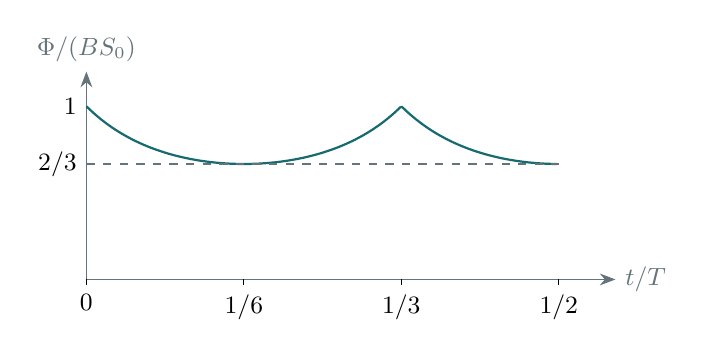
\begin{tikzpicture}[x=12cm,y=2.2cm,font=\small]
\draw[axis] (0,0)--(.56,0) node[right] {$t/T$};\draw[axis] (0,0)--(0,1.2) node[above] {$\Phi/(BS_0)$};
\draw[traj,domain=0:.5,samples=241,variable=\t] plot(\t,{(tan(mod(360*\t,120)/2)+tan(60-mod(360*\t,120)/2))/sqrt(3)});
\foreach \x/\lab in {0/0,.1666667/{1/6},.3333333/{1/3},.5/{1/2}}{\draw (\x,0)--(\x,-.03) node[below] {$\lab$};}
\draw[guide] (0,.6666667)--(.5,.6666667);\node[left] at (0,.6666667) {$2/3$};\node[left] at (0,1) {$1$};
\end{tikzpicture}
\figcaption{解图电3.1C　重叠面积决定磁通曲线。最低点有水平切线，完全重合处曲线左右斜率不同。}
\end{minipage}\end{center}

为求解图电3.1C上的瞬时磁通，取三角形内切圆半径$d=a/(2\sqrt3)$。
两个等边三角形的六条有效边都与此圆相切，其相邻外法线角交替为$\theta$与$2\pi/3-\theta$。
切线多边形面积为内切半径乘周长的一半，故在$0\le\theta\le2\pi/3$内
\[
S(\theta)=3d^2\left[\tan\frac\theta2+\tan\left(\frac\pi3-\frac\theta2\right)\right]
=\frac{a^2}{4}\left[\tan\frac\theta2+\tan\left(\frac\pi3-\frac\theta2\right)\right].
\]
两端为$S_0$，中点为$S_*$，对中点对称；在第一半段斜率为负，后一半段为正。
代$\theta=2\pi t/T$并按$T/3$延拓，就得到C图。曲线的下降段对应正电流，上升段对应反向电流。

解图电3.1B的 $D,E$ 分别将大三角形的两腰三等分。解图电3.1A中三个切角分居三个顶点，每个切角正对转动线框的一条边。对解图电3.1C，可将尖顶看作固定场区和转动线框恰好共用三条边的时刻。经过尖顶时面积连续，前后截去的区域互换，使瞬时电流由斜率的一侧值跳到另一侧值。对任意跨越该点的时间段，电量仍是连续磁通的端点差乘 $-1/R$。


\Needspace{8\baselineskip}

\pdfbookmark[3]{关键洞察}{q1-h5}

\subsection*{关键洞察}

$0,T/3$ 的几何重叠相同，即使每个顶点已移到下一条边的位置。一个磁通周期的净电量为零，对应位于高点两侧的磁通端点相同。只要转动造成非零电流，电流平方的积分就是正值，恒速驱动的机械功补给焦耳热。

\Needspace{8\baselineskip}

\pdfbookmark[3]{易错点}{q1-h6}

\subsection*{易错点}

\begin{itemize}
\item 线框法线固定向外，$\Phi=BS_{\text{重叠}}$。
\item 解图电3.1B的 $DE=a/3$，切去三个角后的面积为 $2S_0/3$。
\item 解图电3.1C在 $T/6$ 到 $T/3$ 之间上升，电流为负。求这段对净电量的贡献，保留负号；求同一时间段的累计电量，取它的绝对值。
\end{itemize}

\Needspace{8\baselineskip}

\pdfbookmark[3]{课堂讲解建议}{q1-h7}

\subsection*{课堂讲解建议}

先让学生在解图电3.1A上把同形的两组三角形连线，写出两个平均值之比。转到B图后，用切角的高和大三角形的高确定面积比。再读解图电3.1C各段斜率的正负，回到变图电3.1V2比较净电量、累计电量。追问把转动方向反过来时，端点的磁通是否改变，让学生在变图电3.1V7上从共同的最高点分别向左和向右走。

\Needspace{18\baselineskip}
\pdfbookmark[3]{变式训练}{q1-h8}

\subsection*{变式训练}

\begin{enumerate}
\item 求 $T/6$ 至 $T/3$ 的平均电流。沿变图电3.1V1的上升段，$\Phi_i=BS_*$、$\Phi_f=BS_0$，故 $q=-B(S_0-S_*)/R=-q_0$。用时 $T/6$，得到
\[\overline I=-\frac{6q_0}{T}=-\frac{\sqrt3 Ba^2}{2RT}.\]
负号表示电流沿 $A\to C\to B\to A$，其磁场指向纸内。
\begin{center}\begin{minipage}{.98\linewidth}\centering
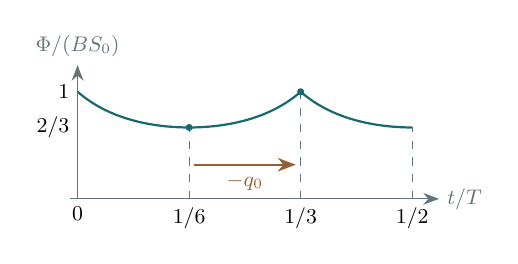
\begin{tikzpicture}[scale=.85,transform shape]
\draw[axis](-.12,0)--(5.4,0)node[right]{$t/T$};
\draw[axis](0,0)--(0,2)node[above]{$\Phi/(BS_0)$};
\draw[traj,domain=0:.5,samples=121,variable=\x]plot({10*\x},{1.6*(tan(mod(360*\x,120)/2)+tan(60-mod(360*\x,120)/2))/sqrt(3)});
\foreach \x/\y/\lab in {0/1.6/0,1.666667/1.066667/{1/6},3.333333/1.6/{1/3},5/1.066667/{1/2}}{\draw[guide](\x,0)--(\x,\y);\node[below]at(\x,0){$\lab$};}
\node[left]at(0,1.6){$1$};\node[left]at(0,1.06667){$2/3$};
\draw[force](1.74,.51)--(3.26,.51)node[midway,below]{$-q_0$};
\fill[accent](1.66667,1.06667)circle(1.5pt) (3.33333,1.6)circle(1.5pt);

\end{tikzpicture}
\figcaption{变图电3.1V1\quad 取右侧上升段两端的磁通差}
\end{minipage}\end{center}
\item 求 $0$ 至 $T/2$ 的累计电量。变图电3.1V2的三个箭头分别代表 $q_0,-q_0,q_0$。各段电流的方向固定，所以
\[Q_{\rm abs}=|q_0|+|-q_0|+|q_0|=3B(S_0-S_*)/R=\sqrt3Ba^2/(4R).\]
带符号相加得到该时间段净电量 $q_0$。
\begin{center}\begin{minipage}{.98\linewidth}\centering
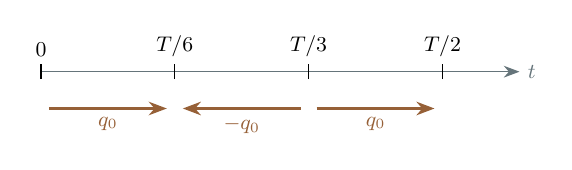
\begin{tikzpicture}[scale=.85,transform shape]
\draw[axis](0,0)--(7.15,0)node[right]{$t$};
\foreach \x/\lab in {0/0,2/{T/6},4/{T/3},6/{T/2}}{\draw (\x,-.11)--(\x,.11);\node[above]at(\x,.1){$\lab$};}
\draw[force](.12,-.55)--(1.88,-.55)node[midway,below]{$q_0$};
\draw[force](3.88,-.55)--(2.12,-.55)node[midway,below]{$-q_0$};
\draw[force](4.12,-.55)--(5.88,-.55)node[midway,below]{$q_0$};
\end{tikzpicture}
\figcaption{变图电3.1V2\quad 沿时间轴分段，箭头的正负对应电流的绕行方向}
\end{minipage}\end{center}
\item 电阻改为 $2R$，转速保持。磁通由几何决定，因此 $I_{2R}(t)=-\dot\Phi/(2R)=I_R(t)/2$。变图电3.1V3以 $I_*=\pi Ba^2/(R T)\times3/4$ 为标度，实、虚曲线的纵坐标之比处处为2，过零时刻相同。两次平均电流和累计电量均减半。瞬时热功率 $2R I_{2R}^2=R I_R^2/2$，故同一用时的焦耳热也减半。
\begin{center}\begin{minipage}{.98\linewidth}\centering
\begin{tikzpicture}[scale=.85,transform shape]
\draw[axis](0,0)--(5.5,0)node[right]{$t/T$};
\draw[axis](0,-1.46)--(0,1.68)node[above]{$I/I_*$};
\draw[guide](0,1.5)--(5,1.5);
\node[left]at(0,1.5){$1$};
\foreach \j in {0,1}{
\draw[traj,domain=0:1.666666,samples=37,variable=\x]plot({\x+3.333333*\j},{1.5*((cos(60-18*\x))^(-2)-(cos(18*\x))^(-2))/3});
\draw[object,dashed,domain=0:1.666666,samples=37,variable=\x]plot({\x+3.333333*\j},{.75*((cos(60-18*\x))^(-2)-(cos(18*\x))^(-2))/3});
}
\draw[traj,domain=1.666667:3.333333,samples=37,variable=\x]plot(\x,{1.5*((cos(60-18*\x))^(-2)-(cos(18*\x))^(-2))/3});
\draw[object,dashed,domain=1.666667:3.333333,samples=37,variable=\x]plot(\x,{.75*((cos(60-18*\x))^(-2)-(cos(18*\x))^(-2))/3});
\node[right]at(4.9,.94){$R$（实线）};
\node[right]at(4.9,.52){$2R$（虚线）};

\end{tikzpicture}
\figcaption{变图电3.1V3\quad 阻值加倍时，电流曲线的纵坐标缩为一半}
\end{minipage}\end{center}
\item 保留自感 $L$，求平均电流的端点表达式。回路方程为 $L\dot I+RI=-\dot\Phi$。把变图电3.1V4纵轴读数记为 $F=LI+\Phi$，则 $\dot F=-RI$，从 $t_i$ 积到 $t_f$，
\[\overline I=-\frac{\Phi_f-\Phi_i+L(I_f-I_i)}{R(t_f-t_i)}.\]
半段旋转的电量同时随外磁通和端点电流变化。周期稳态取一整周期，图上两个端点的 $F$ 相同，所以该周期净电量为零。
\begin{center}\begin{minipage}{.98\linewidth}\centering
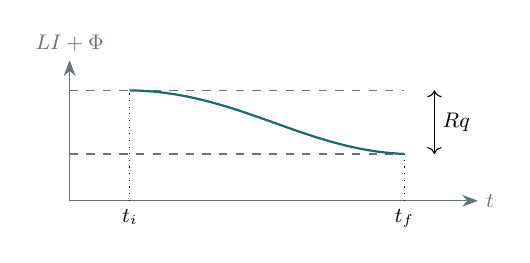
\begin{tikzpicture}[scale=.85,transform shape]
\draw[axis](0,0)--(6.1,0)node[right]{$t$};
\draw[axis](0,0)--(0,2.1)node[above]{$LI+\Phi$};
\draw[guide](0,1.65)--(5,1.65);
\draw[guide](0,.70)--(5,.70);
\draw[traj](.9,1.65)..controls(2.5,1.63)and(3.5,.76)..(5,.70);
\draw[dotted](.9,0)--(.9,1.65)(5,0)--(5,.70);
\draw[<->](5.45,.70)--(5.45,1.65)node[midway,right]{$Rq$};
\node[below]at(.9,0){$t_i$};\node[below]at(5,0){$t_f$};
\end{tikzpicture}
\figcaption{变图电3.1V4\quad 净电量取总磁通链的端点差}
\end{minipage}\end{center}
\item 改用非匀速转动，从重合分别到 $\pi/3,\pi$，用时 $t_1,t_2$。按变图电3.1V5的两条转角曲线，两次终角相差 $2\pi/3$，端点磁通均为 $BS_*$。积分后各得 $q_0$。于是 $\overline I_1=q_0/t_1$，$\overline I_2=q_0/t_2$，比值 $\overline I_2/\overline I_1=t_1/t_2$。匀速的两个时间才有 $t_2=3t_1$。
\begin{center}\begin{minipage}{.98\linewidth}\centering
\begin{tikzpicture}[scale=.85,transform shape]
\draw[axis](0,0)--(6.6,0)node[right]{$t$};
\draw[axis](0,0)--(0,3.35)node[above]{$\theta$};
\draw[traj](0,0) .. controls(1.14,.17)and(1.96,.48)..(2.14,1.03);
\draw[object,dashed](0,0)..controls(1.2,1.95)and(3.7,2.27)..(5.75,3.09);
\draw[guide](0,1.03)--(2.14,1.03)--(2.14,0)(0,3.09)--(5.75,3.09)--(5.75,0);
\node[left]at(0,1.03){$\pi/3$};\node[left]at(0,3.09){$\pi$};
\node[below]at(2.14,0){$t_1$};\node[below]at(5.75,0){$t_2$};
\end{tikzpicture}
\figcaption{变图电3.1V5\quad 示例中的两种转速历史给不同的到达时间}
\end{minipage}\end{center}
\item 求任意两转角间的净电量。变图电3.1V6中，先将 $\theta_i,\theta_f$ 各自按 $2\pi/3$ 归约，再用标准解法的面积函数读出两点面积：
\[q=\frac{B}{R}[S(\theta_i)-S(\theta_f)].\]
在这幅图中 $\theta_i=\pi/6$、$\theta_f=53\pi/60$，后一角归约为 $13\pi/60$，所以磁通略减，净电量为正。如果求累计电量，以图中的极值 $\theta=k\pi/3$ 为分段点，将各段面积差取绝对值后相加，再乘 $B/R$。
\begin{center}\begin{minipage}{.98\linewidth}\centering
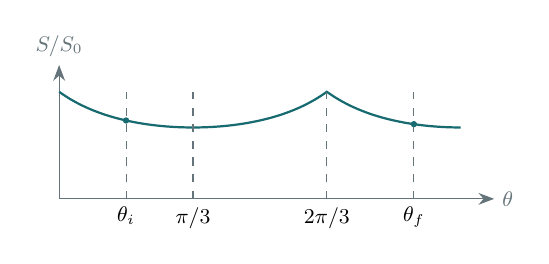
\begin{tikzpicture}[scale=.85,transform shape]
\draw[axis](0,0)--(6.5,0)node[right]{$\theta$};
\draw[axis](0,0)--(0,2)node[above]{$S/S_0$};
\draw[traj,domain=0:3,samples=145,variable=\x]plot({2*\x},{1.6*(tan(30*mod(\x,2))+tan(60-30*mod(\x,2)))/sqrt(3)});
\foreach \x/\lab in {1.0/{\theta_i},2/{\pi/3},4/{2\pi/3},5.3/{\theta_f}}{\draw[guide](\x,0)--(\x,1.6);\node[below]at(\x,0){$\lab$};}
\fill[accent](1,1.17128)circle(1.35pt) (5.3,1.116087)circle(1.35pt);

\end{tikzpicture}
\figcaption{变图电3.1V6\quad 跨越多个升降段时，以两端面积求净电量}
\end{minipage}\end{center}
\item 从完全重合反向起转。变图电3.1V7以顺时针转角为正；两侧有 $S(-\theta)=S(\theta)$。从 $\theta=0$ 沿任一箭头出发，重叠面积均下降，故 $I=-(B/R)\dot S>0$。若转到同一个非极值角时让角速度换号，则由 $I=-(B/R)S'(\theta)\dot\theta$，该时刻的电流换号。
\begin{center}\begin{minipage}{.98\linewidth}\centering
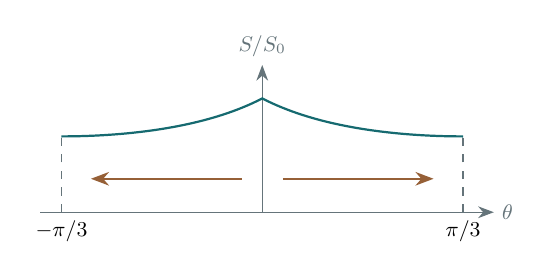
\begin{tikzpicture}[scale=.85,transform shape]
\draw[axis](-3.32,0)--(3.46,0)node[right]{$\theta$};
\draw[axis](0,0)--(0,2.2)node[above]{$S/S_0$};
\draw[traj,domain=-3:3,samples=83,variable=\x]plot(\x,{1.7*(tan(10*abs(\x))+tan(60-10*abs(\x)))/sqrt(3)});
\draw[force](-.31,.5)--(-2.56,.5);
\draw[force](.31,.5)--(2.56,.5);
\draw[guide](-3,0)--(-3,1.133333)(3,0)--(3,1.133333);
\node[below]at(-3,0){$-\pi/3$};\node[below]at(3,0){$\pi/3$};

\end{tikzpicture}
\figcaption{变图电3.1V7\quad 从完全重合向任一侧转，重叠面积都先减小}
\end{minipage}\end{center}
\item 仅由第一段净电量给焦耳热的下界。变图电3.1V8中，面积相等的虚线高度是 $\overline I_1=q_0/\Delta t$，其中 $\Delta t=T/6$。将电流分为 $\overline I_1$ 和积分为零的起伏，则
\[R\int_0^{\Delta t}I^2\dd t
=R\Delta t\,\overline I_1^2+R\int_0^{\Delta t}(I-\overline I_1)^2\dd t
>\frac{R q_0^2}{\Delta t}=\frac{B^2a^4}{8RT}.\]
磁通在区间末端有水平切线，实际电流从非零值降到零，起伏项为正。图中 $I_*$ 是第一段起始的右极限。
\begin{center}\begin{minipage}{.98\linewidth}\centering
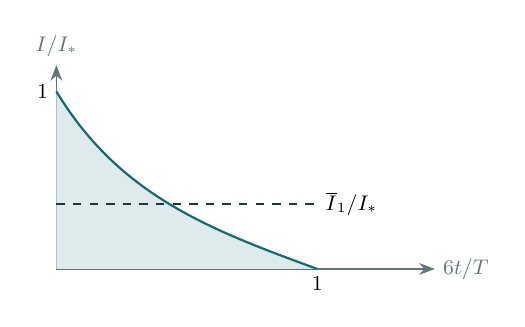
\begin{tikzpicture}[scale=.85,transform shape]
\begin{scope}[x=3.9cm,y=2.65cm]
\draw[axis](0,0)--(1.45,0)node[right]{$6t/T$};
\draw[axis](0,0)--(0,1.15)node[above]{$I/I_*$};
\fill[accent!14](0,0)--plot[domain=0:1,samples=55,variable=\x](\x,{((cos(60-30*\x))^(-2)-(cos(30*\x))^(-2))/3})--cycle;
\draw[traj,domain=0:1,samples=55,variable=\x]plot(\x,{((cos(60-30*\x))^(-2)-(cos(30*\x))^(-2))/3});
\draw[object,dashed](0,{2*sqrt(3)/(3*pi)})--(1,{2*sqrt(3)/(3*pi)});
\node[right]at(1,{2*sqrt(3)/(3*pi)}){$\overline I_1/I_*$};
\node[left]at(0,1){$1$};
\node[below]at(1,0){$1$};
\end{scope}
\end{tikzpicture}
\figcaption{变图电3.1V8\quad 等高虚线与曲线给同一净电量，起伏使热量增加}
\end{minipage}\end{center}
\end{enumerate}

\clearpage

\pdfbookmark[2]{第 2 题 恒力收缩导线圆圈的闭合时间}{q2}

\section*{第 2 题\quad 恒力收缩导线圆圈的闭合时间}\label{q:2}

柔软导体回路$ABCDA$的总电阻恒为$R$，其中$AB$段的一部分绕成初始半径$r_0$的圆圈，圆圈处于垂直其平面的匀强磁场$B$中。$B$端固定，$C,D$端自由；沿$BA$方向对$A$端施加恒力$F$，使圆圈缓慢缩小并始终保持圆形。忽略导线惯性、自感、弹性储能和一切机械阻力，圆圈以外部分的磁通变化忽略不计。求半径缩至零的形式闭合时间$T$。

\begin{center}\begin{minipage}{.98\linewidth}\centering
\begin{tikzpicture}[scale=.85]

\draw[object] (-2,1.8) node[above left]{$B$（固定）}--(-.65,1.8)
.. controls(-.4,1.8) and(-.45,1.15)..(.17365,.98481)
arc(80:-260:1)
.. controls(.05,1.15) and(.35,1.8)..(.65,1.8)--(3.8,1.8) node[above]{$A$};
\draw[object] (3.8,1.8)--(3.8,-1.5) node[right]{$D$}--(-2,-1.5) node[left]{$C$}--(-2,1.8);
\draw[force] (4.1,1.8)--(5.4,1.8) node[right]{$F$};
\draw[axis] (0,0)--(-.707,-.707) node[midway,below]{$r_0$};\node at(.3,.2){$\odot B$};

\end{tikzpicture}\figcaption{图电3.2\quad 圆圈串在$AB$软线段中，交叉处不电接触；外部回路示意。}\end{minipage}\end{center}

\Needspace{8\baselineskip}

\pdfbookmark[3]{题型定位}{q2-h0}

\subsection*{题型定位}

恒力从软导线圆圈拉出线长，长度约束与电磁耗散共同确定收缩速度。题设的无惯性、无自感模型给出半径降至零的形式时间。

\Needspace{8\baselineskip}

\pdfbookmark[3]{知识点}{q2-h1}

\subsection*{知识点}

导线长度固定时 $\dd x=-2\pi\dd r$，回路磁通为 $B\pi r^2$。用法拉第定律求 $\mathcal E=Br\dot x$。由 $F\dot x=I^2R$ 和 $I=\mathcal E/R$ 求收缩速度，也可先写 $F=BrI$。

\Needspace{8\baselineskip}

\pdfbookmark[3]{物理图像}{q2-h2}

\subsection*{物理图像}

解图电3.2A中，圆周缩短的线长进入切向直线段。电流产生向外磁场，小弧受力向外，与张力的径向合量平衡。图B的直线画的是 $r^3$，图C分别画以各自初值归一化的 $I$ 与 $-\dot r$。

\Needspace{8\baselineskip}

\pdfbookmark[3]{解题入口}{q2-h3}

\subsection*{解题入口}

把图A的长度关系代入电动势，用 $F\dot x$ 与 $I^2R$ 相等求 $\dot x$。在 $r>0$ 的收缩段，$\dot x>0$，消去一因子 $\dot x$ 后得到 $\dot r\propto-r^{-2}$。以 $r_0$ 为下限分离变量。

\Needspace{18\baselineskip}
\pdfbookmark[3]{标准解法}{q2-h4}

\subsection*{标准解法}

解图电3.2A用$x$标记$A$端拉出的导线长度。圆圈的周长缩短多少，直线段就增加多少，故
\[
\dd x=-\dd(2\pi r)=-2\pi\dd r,\qquad \dot r<0.
\]
半径每减小一单位长度，直线段的增长量为 $2\pi$ 单位长度。

\begin{center}\begin{minipage}{.98\linewidth}\centering
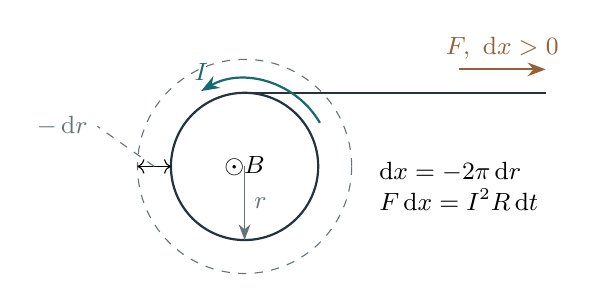
\begin{tikzpicture}[scale=.85]

\draw[guide] (0,0) circle(1.6);\draw[object] (0,0) circle(1.1);
\draw[axis] (0,0)--(0,-1.1) node[midway,right]{$r$};
\draw[<->] (-1.6,0)--(-1.1,0);\draw[guide] (-1.35,0)--(-2.2,.6) node[left]{$-\dd r$};
\draw[object] (0,1.1)--(4.5,1.1);\draw[force] (3.2,1.45)--(4.5,1.45) node[midway,above]{$F,\ \dd x>0$};
\draw[motion] (30:1.3) arc(30:120:1.3) node[above]{$I$};\node at(0,0){$\odot B$};
\node[align=left] at(3.2,-.3){$\dd x=-2\pi\dd r$\\$F\dd x=I^2R\dd t$};

\end{tikzpicture}\figcaption{解图电3.2A\quad 圆周缩短转为拉出长度；电流阻碍磁通减少。}\end{minipage}\end{center}

取圆圈内磁通的正方向与$B$一致。圆圈缩小时磁通减少，感应电流产生同向磁场。电动势、电流的大小分别为
\[
\mathcal E=-\frac{\dd(B\pi r^2)}{\dd t}
=-2\pi Br\dot r,\qquad
I=-\frac{2\pi Br}{R}\dot r.
\]
在规定的缓慢、无惯性模型中，机械功全部成为焦耳热：
\[
F\dd x=I^2R\dd t.
\]
代入几何约束与电流，在$r>0$的收缩阶段约去非零的$\dot r$，得到
\[
-2\pi F\dot r=\frac{4\pi^2B^2r^2}{R}\dot r^2,
\qquad
\dot r=-\frac{FR}{2\pi B^2r^2}.
\]
分离变量并使用$r(0)=r_0$：
\[
\int_{r_0}^{r}u^2\dd u=-\frac{FR}{2\pi B^2}\int_0^t\dd t,
\quad
r^3=r_0^3-\frac{3FR}{2\pi B^2}t.
\]
令$r=0$，得到
\[
\boxed{T=\frac{2\pi B^2r_0^3}{3FR}},\qquad
r(t)=r_0\left(1-\frac tT\right)^{1/3}.
\]
整个过程中，$A$ 端拉出长度$2\pi r_0$，因此总焦耳热为$Q=2\pi Fr_0$。由上式也得$I=F/(Br)$：临近$r=0$时电流和收缩速度发散。上式中的 $T$ 是准静态方程积分到 $r=0$ 的形式闭合时间。若只算到有限的小半径 $\varepsilon$，形式上继续收缩到零的时间为 $T(\varepsilon/r_0)^3$。

收缩末端的速度虽发散，电量与总热量的积分仍有限。将$\dd t=-2\pi B^2r^2\dd r/(FR)$代入，可得
\[
q_{\rm tr}=\int_0^T I\dd t
=-\frac{2\pi B}{R}\int_{r_0}^{0}r\dd r
=\frac{B\pi r_0^2}{R},
\]
\[
\int_0^T I^2R\dd t
=-2\pi F\int_{r_0}^{0}\dd r=2\pi Fr_0.
\]
电量等于磁通减少量除以 $R$，而热量等于恒力乘整个拉出长度。解图电3.2B把运动写成$r^3$的直线规律，便于看出后段所占的时间。

\begin{center}\begin{minipage}{.98\linewidth}\centering
\begin{tikzpicture}[scale=.85]

\draw[axis](0,0)--(5.2,0) node[right]{$t/T$};\draw[axis](0,0)--(0,2.8) node[above]{$r^3/r_0^3$};
\draw[traj](0,2.2)--(4.4,0);\node[left] at(0,2.2){$1$};\node[below right] at(4.4,0){$1$};
\draw[guide](3.85,0)--(3.85,.275)--(0,.275);\fill(3.85,.275) circle(1.5pt);
\node[below left] at(3.85,0){$7/8$};\node[left] at(0,.275){$1/8$};
\node[align=left] at(8,1.5){$r=r_0/2$时$t=7T/8$\\$r^3=r_0^3(1-t/T)$\\末段做功占总功一半};

\end{tikzpicture}\figcaption{解图电3.2B\quad 半径的立方随时间线性下降，半径的减小速率随时间增大。}\end{minipage}\end{center}

当 $r=r_0/2$ 时，$t/T=1-(1/2)^3=7/8$。此后在总历时的最后 $1/8$ 内拉出一半圆周长度，恒力在这段所做的功占总功的一半。

\begin{center}\begin{minipage}{.97\linewidth}\centering
\begin{tikzpicture}[x=1cm,y=1cm,font=\small]
\foreach \xx/\lab/\pow in {0/{I/I_0}/{1/3},4.5/{(-\dot r)/(-\dot r_0)}/{2/3}}{\begin{scope}[xshift=\xx cm]
\draw[axis] (0,0)--(3.2,0) node[right] {$t/T$};\draw[axis] (0,0)--(0,3) node[above] {$\lab$};
\draw[traj,domain=0:.88,samples=90,variable=\t] plot({3*\t},{.6*(1-\t)^(-\pow)});
\draw[guide] (3,0)--(3,2.85);\node[below] at (3,0) {$1$};\node[left] at (0,.6) {$1$};\end{scope}}
\end{tikzpicture}
\figcaption{解图电3.2C　用各自初值归一化的电流与收缩速率；均沿实际幂律绘制到$t/T=0.88$，虚线表示形式闭合时刻，曲线在此前已显示加速。}
\end{minipage}\end{center}

从圆圈截取张角为 $\dd\phi$ 的小弧。沿正向的感应电流在向外磁场中使小弧受到向外的磁力 $IBr\dd\phi$。软线张力近似等于端拉力 $F$ 时，小弧两端的切向张力合成向内的径向分量 $F\dd\phi$。无惯性的圆形收线模型给 $F=IBr$，说明同一个拉力在较小半径处需要较大的电流来平衡。

解图电3.2C由$r/r_0=(1-t/T)^{1/3}$直接给出
\[
\frac{I}{I_0}=(1-t/T)^{-1/3},\qquad
\frac{-\dot r}{-\dot r_0}=(1-t/T)^{-2/3},\qquad I_0=\frac{F}{Br_0}.
\]
临近 $T$，焦耳热功率按 $(T-t)^{-2/3}$ 增大。积分 $\int_{t_*}^T(T-t)^{-2/3}\dd t=3(T-t_*)^{1/3}$ 随余下时间 $T-t_*$ 减小而趋零。图B给出 $r_0/2$ 以下的收缩时间为 $T/8$。图C的电流迅速增大，热功率的积分在这段达到总热量的一半。这里的上升曲线适用于导线仍可视为圆形，且惯性与自感相对较小的阶段。


\Needspace{8\baselineskip}

\pdfbookmark[3]{关键洞察}{q2-h5}

\subsection*{关键洞察}

单位拉出长度的功为 $F$，单位半径减小量对应热量 $2\pi F$。与此相对，每缩短同样的半径，用时随 $r^2$ 减小。定半径下，加大磁场降低收缩速度，但整个过程的拉出长度和总热量与 $B$ 无关。

\Needspace{8\baselineskip}

\pdfbookmark[3]{易错点}{q2-h6}

\subsection*{易错点}

\begin{itemize}
\item 连续收缩对应 $\dot r<0$、$\dot x>0$。圆周导线减少的长度是 $-2\pi\dd r$。
\item $R$ 是整个闭合回路的电阻。线从圆形部分移到直线部分后仍在回路中。
\item 时间元含 $r^2\dd r$，所以 $T$ 随初始半径的立方变化。
\end{itemize}

\Needspace{8\baselineskip}

\pdfbookmark[3]{课堂讲解建议}{q2-h7}

\subsection*{课堂讲解建议}

先让学生在解图电3.2A上描出拉出前后导线的轮廓，指出线长从何处移到何处。到解图电3.2B读 $r=r_0/2$ 对应的时间，再问同一时刻拉力已经做了多少功。接着用变图电3.2V5分别估计小半径阶段剩余的时间、电量和发热量，说明三条曲线各自来自哪一个积分。

\Needspace{18\baselineskip}
\pdfbookmark[3]{变式训练}{q2-h8}

\subsection*{变式训练}

\begin{enumerate}
\item 求收至半径 $r_0/2$ 的历时。用变图电3.2V1的横坐标 $r/r_0$ 读出 $t/T=1-(r/r_0)^3$。当 $r=r_0/2$，历时为 $7T/8$。若只拉出初始周长的四分之一，$\dd x=-2\pi\dd r$ 给 $r=3r_0/4$，代入得到 $t/T=1-27/64=37/64$。
\begin{center}\begin{minipage}{.98\linewidth}\centering
\begin{tikzpicture}[scale=.85,transform shape]
\begin{scope}[x=5.65cm,y=2.96cm]
\draw[axis](0,0)--(1.19,0)node[right]{$r/r_0$};
\draw[axis](0,0)--(0,1.16)node[above]{$t/T$};
\node[below left]at(0,0){$0$};\node[below]at(1,0){$1$};\node[left]at(0,1){$1$};
\draw[traj,domain=0:1,samples=64]plot(\x,{1-\x^3});
\foreach \x/\y/\lab in {.5/.875/{7/8},.75/.578125/{37/64}}{
\draw[guide](0,\y)--(\x,\y)--(\x,0);
\fill[accent](\x,\y)circle(1.45pt);\node[left]at(0,\y){$\lab$};\node[below]at(\x,0){$\x$};}
\end{scope}
\end{tikzpicture}
\figcaption{变图电3.2V1\quad 从初始半径收缩至指定半径时的历时}
\end{minipage}\end{center}
\item $F,R,r_0$ 固定，磁场增为 $2B$。变图电3.2V2以旧场强下的初始电流 $I_0=F/(Br_0)$ 为尺度。同一半径处 $I=F/(Br)$ 降为一半，$-\dot r=FR/(2\pi B^2r^2)$ 降为四分之一，故闭合时间为 $4T$。整段位移为 $2\pi r_0$，总热量仍为 $2\pi Fr_0$。电量由磁通差除以电阻，随 $B$ 加倍。
\begin{center}\begin{minipage}{.98\linewidth}\centering
\begin{tikzpicture}[scale=.85,transform shape]
\begin{scope}[x=5.65cm,y=1.36cm]
\draw[axis](0,0)--(1.19,0)node[right]{$r/r_0$};
\draw[axis](0,0)--(0,2.36)node[above]{$I/I_0$};
\node[below left]at(0,0){$0$};\node[below]at(1,0){$1$};\node[left]at(0,1){$1$};
\draw[traj,domain=.47:1,samples=68]plot(\x,{1/\x});
\draw[object,dashed,domain=.47:1,samples=68]plot(\x,{.5/\x});
\draw[guide](.8,0)--(.8,1.25);\fill[accent](.8,1.25)circle(1.4pt) (.8,.625)circle(1.4pt);
\node[above right]at(.55,1.83){场强 $B$};
\node[below left]at(.81,.55){场强 $2B$};
\end{scope}
\end{tikzpicture}
\figcaption{变图电3.2V2\quad 在同一半径比较两种场强的电流}
\end{minipage}\end{center}
\item 将拉力改为 $F(r)>0$，从 $\dot r=-RF(r)/(2\pi B^2r^2)$ 得
\[T=\int_0^{r_0}\frac{2\pi B^2r^2}{RF(r)}\dd r.\]
取 $F=kr$ 后，变图电3.2V3的直线给 $\left|\dd t/\dd r\right|\propto r$，积分得 $T=\pi B^2r_0^2/(kR)$。若在零附近 $F(r)\sim kr^p$，时间元随 $r^{2-p}$ 变，闭合时间有限的条件是 $p<3$；图中的 $p=3$ 恰给对数发散。
\begin{center}\begin{minipage}{.98\linewidth}\centering
\begin{tikzpicture}[scale=.85,transform shape]
\begin{scope}[x=5.65cm,y=1.45cm]
\draw[axis](0,0)--(1.19,0)node[right]{$r/r_0$};
\draw[axis](0,0)--(0,2.96)node[above]{近零端的时间元（按各自尺度归一化）};
\node[below left]at(0,0){$0$};\node[below]at(1,0){$1$};\node[left]at(0,1){$1$};
\draw[traj,domain=.13:1,samples=56]plot(\x,{\x});
\draw[object,dashed,domain=.36:1,samples=56]plot(\x,{1/\x});
\node[above left]at(.87,.89){$p=1$};
\node[above right]at(.51,1.92){$p=3$};
\end{scope}
\end{tikzpicture}
\figcaption{变图电3.2V3\quad 时间元随半径变化，$p=3$ 时的曲线为双曲线}
\end{minipage}\end{center}
\item 以恒定线速度 $u$ 拉动导线，$\dot r=-u/(2\pi)$，故 $r=r_0-ut/(2\pi)$。变图电3.2V4两条曲线分别为 $\mathcal E=Bru$ 和 $F=\mathcal E^2/(Ru)=B^2r^2u/R$ 的归一化值。半径减半时，电动势减半，拉力降至四分之一。闭合用时由放完总线长决定，为 $2\pi r_0/u$。
\begin{center}\begin{minipage}{.98\linewidth}\centering
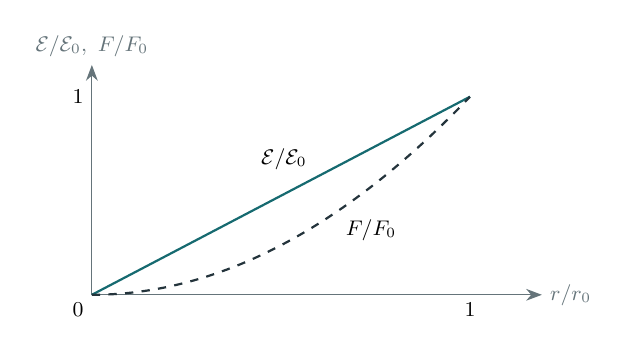
\begin{tikzpicture}[scale=.85,transform shape]
\begin{scope}[x=5.65cm,y=2.96cm]
\draw[axis](0,0)--(1.19,0)node[right]{$r/r_0$};
\draw[axis](0,0)--(0,1.16)node[above]{$\mathcal E/\mathcal E_0,\ F/F_0$};
\node[below left]at(0,0){$0$};\node[below]at(1,0){$1$};\node[left]at(0,1){$1$};
\draw[traj](0,0)--(1,1);
\draw[object,dashed,domain=0:1,samples=57]plot(\x,{\x*\x});
\node[above left]at(.59,.59){$\mathcal E/\mathcal E_0$};
\node[below right]at(.65,.423){$F/F_0$};
\end{scope}
\end{tikzpicture}
\figcaption{变图电3.2V4\quad 恒拉线速度下，半径同时确定电动势和拉力}
\end{minipage}\end{center}
\item 收至 $r=\varepsilon$ 时停止。由立方时间关系、端点磁通差和拉出线长，依次得到
\[t_\varepsilon=T[1-(\varepsilon/r_0)^3],\qquad q_\varepsilon=\pi B(r_0^2-\varepsilon^2)/R,\qquad Q_\varepsilon=2\pi F(r_0-\varepsilon).\]
变图电3.2V5画的是三项余量占全程总量的比例，横坐标固定为 $\varepsilon/r_0$，三条曲线分别给三次方、平方和一次方。
\begin{center}\begin{minipage}{.98\linewidth}\centering
\begin{tikzpicture}[scale=.85,transform shape]
\begin{scope}[x=5.65cm,y=2.96cm]
\draw[axis](0,0)--(1.19,0)node[right]{$r/r_0$};
\draw[axis](0,0)--(0,1.16)node[above]{余量占各自总量的比例};
\node[below left]at(0,0){$0$};\node[below]at(1,0){$1$};\node[left]at(0,1){$1$};
\draw[object,dashed](0,0)--(1,1);
\draw[traj,domain=0:1,samples=56]plot(\x,{\x*\x});
\draw[thick,warm,domain=0:1,samples=56]plot(\x,{\x^3});
\node[left]at(.6,.62){热量};
\node[above right]at(.53,.27){电量};
\node[below right]at(.64,.19){时间};
\draw[guide](.39,0)--(.39,.39);\node[below]at(.39,0){$\varepsilon/r_0$};
\end{scope}
\end{tikzpicture}
\figcaption{变图电3.2V5\quad 截止半径以下尚余的时间、电量和热量}
\end{minipage}\end{center}
\item 若力和电阻都随半径变化，在每个半径仍用 $F(r)\dot x=[Br\dot x]^2/R(r)$，得
\[\dot r=-\frac{F(r)R(r)}{2\pi B^2r^2},\qquad T=\int_0^{r_0}\frac{2\pi B^2r^2}{F(r)R(r)}\dd r.\]
变图电3.2V6以 $F(r)=kr$ 为例，着色面积对应 $R(r)=R_0(1+r/r_0)$，于是 $T=[2\pi B^2r_0^2/(kR_0)](1-\ln2)$。零附近的时间元与 $r$ 成正比，可积分。随半径变化的电阻在电量积分中保留为 $q=2\pi B\int_0^{r_0}r\dd r/R(r)$。
\begin{center}\begin{minipage}{.98\linewidth}\centering
\begin{tikzpicture}[scale=.85,transform shape]
\begin{scope}[x=5.65cm,y=2.96cm]
\draw[axis](0,0)--(1.19,0)node[right]{$r/r_0$};
\draw[axis](0,0)--(0,1.16)node[above]{$\left|\dd t/\dd r\right|$（相对尺度）};
\node[below left]at(0,0){$0$};\node[below]at(1,0){$1$};\node[left]at(0,1){$1$};
\fill[accent!14](0,0)--plot[domain=0:1,samples=62](\x,{\x/(1+\x)})--(1,0)--cycle;
\draw[traj,domain=0:1,samples=62]plot(\x,{\x/(1+\x)});
\draw[object,dashed](0,0)--(1,1);
\node[above left]at(.84,.84){$R=R_0$};
\node[below right]at(.53,.31){$R=R_0(1+r/r_0)$};
\end{scope}
\end{tikzpicture}
\figcaption{变图电3.2V6\quad 同为 $F=kr$，增加电阻缩小时间积分的面积}
\end{minipage}\end{center}
\item 改由恒定机械功率 $P$ 驱动。$P=(Br\dot x)^2/R$ 给 $\dot r=-\sqrt{PR}/(2\pi Br)$。乘以 $2r$ 后积分，$r^2=r_0^2-\sqrt{PR}\,t/(\pi B)$，所以
\[T_P=\frac{\pi Br_0^2}{\sqrt{PR}}.\]
变图电3.2V7的水平线取 $I_*=\sqrt{P/R}$ 为尺度，斜线表示 $r^2/r_0^2$。总热量为 $PT_P$。
\begin{center}\begin{minipage}{.98\linewidth}\centering
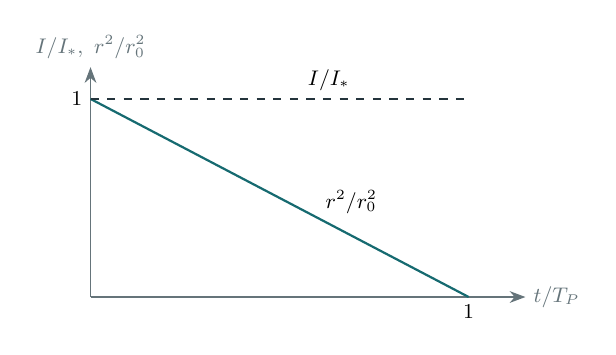
\begin{tikzpicture}[scale=.85,transform shape]
\begin{scope}[x=5.65cm,y=2.96cm]
\draw[axis](0,0)--(1.15,0)node[right]{$t/T_P$};
\draw[axis](0,0)--(0,1.16)node[above]{$I/I_* ,\ r^2/r_0^2$};
\draw[traj](0,1)--(1,0);
\draw[object,dashed](0,1)--(1,1);
\node[above]at(.63,1){$I/I_*$};
\node[above right]at(.6,.38){$r^2/r_0^2$};
\node[below]at(1,0){$1$};\node[left]at(0,1){$1$};
\end{scope}
\end{tikzpicture}
\figcaption{变图电3.2V7\quad 恒功率时电流保持恒定，半径的平方线性下降}
\end{minipage}\end{center}
\item 串联固定电阻 $R_c$，按变图电3.2V8整个回路的电阻为 $R+R_c$。用收缩微分方程得 $T_c=2\pi B^2r_0^3/[3F(R+R_c)]$。给定 $r,F$ 时由 $I=F/(Br)$ 确定电流，欧姆定律要求更大电动势，故运动加快。两电阻始终通过同一电流，积分 $I^2R$ 和 $I^2R_c$ 得
\[Q_R=2\pi Fr_0\frac{R}{R+R_c},\qquad Q_c=2\pi Fr_0\frac{R_c}{R+R_c}.\]
\begin{center}\begin{minipage}{.98\linewidth}\centering
\begin{tikzpicture}[scale=.85,transform shape]
\draw[object](-.8,0)--(0,0)--(.46,0)--(.65,.24)--(.9,-.24)--(1.15,.24)--(1.4,-.24)--(1.64,0)--(3.3,0)--(3.55,.24)--(3.8,-.24)--(4.05,.24)--(4.3,-.24)--(4.57,0)--(5.52,0);
\draw[object](-.8,0)--(-.8,-1.25)--(5.52,-1.25)--(5.52,0);
\node[above]at(1.05,.27){$R$};\node[above]at(4.04,.27){$R_c$};
\draw[force](1.82,-1)--(3.58,-1)node[midway,above]{$I$};
\node[above]at(2.6,.73){耗散功率 $I^2R$ 和 $I^2R_c$};
\end{tikzpicture}
\figcaption{变图电3.2V8\quad 串联电阻通过同一电流，按阻值分配热量}
\end{minipage}\end{center}
\end{enumerate}

\clearpage

\pdfbookmark[2]{第 3 题 铜环倾倒时的磁阻尼与能量}{q3}

\section*{第 3 题\quad 铜环倾倒时的磁阻尼与能量}\label{q:3}

细铜圆环的主半径$r_1=1.0\,\mathrm{cm}$，圆形导线截面半径$r_2=1.0\,\mathrm{mm}$。圆环竖放，底部有光滑固定栓限制滑动，使它可绕经过最低点的水平切线轴倾倒。竖直向上匀强磁场$B=1.0\,\mathrm T$。圆环由与竖直方向夹角$\theta_0=1.0\,\mathrm{rad}$的位置静止释放，最后到达水平位置。铜的电导率$\sigma=6.25\times10^7\,\mathrm{S/m}$，密度$\rho=8.93\times10^3\,\mathrm{kg/m^3}$，取$g=9.80\,\mathrm{m/s^2}$，忽略自感、空气阻力及接触耗散。
\begin{enumerate}
\item 通过估算和能量关系，判断重力势能如何分配；说明平均转速能否直接估计倒地瞬间的转动动能。
\item 在忽略角加速度项的准静态近似中，令磁阻力矩与重力矩相等，求从一般初始角$0<\theta_0<\pi/2$到水平位置的时间，并计算$\theta_0=1.0\,\mathrm{rad}$的结果。讨论近似的适用范围。
\end{enumerate}

\begin{center}\begin{minipage}{.98\linewidth}\centering
\begin{tikzpicture}[scale=.85]

\draw[object] (-1,0)--(3.2,0);\fill(0,0) circle(2pt) node[below]{$P$（栓轴）};
\draw[guide] (0,0)--(0,2.8);\draw[object,very thick] (0,0)--(2.6927,1.7290);
\fill(1.3464,.8645) circle(2pt) node[above]{$G$};\node at(.65,.18){$r_1$};
\draw (0,.85) arc(90:32.7042:.85);\node at(.48,1.02){$\theta_0$};
\foreach \x in {4,4.7,5.4}{\draw[motion] (\x,.2)--(\x,2.8);}\node at(4.7,3.2){$B$};
\node at(-.9,2.3){侧视};\node at(7.5,2.2){导线截面};\draw[object] (7.5,1.1) circle(.4);
\draw[axis] (7.5,1.1)--(7.9,1.1) node[midway,above]{$r_2$};

\end{tikzpicture}\figcaption{图电3.3\quad 初始环面倾角为$1.0\,\mathrm{rad}$；重心$G$距栓轴为$r_1$。}\end{minipage}\end{center}

\Needspace{8\baselineskip}

\pdfbookmark[3]{题型定位}{q3-h0}

\subsection*{题型定位}

圆环绕下方切线轴倾倒，磁通变化引起的感应电流产生阻尼力矩。完整方程确定能量分配，略去角加速度项则给准静态时间。

\Needspace{8\baselineskip}

\pdfbookmark[3]{知识点}{q3-h1}

\subsection*{知识点}

细圆环关于直径轴的惯量为 $mr_1^2/2$，平移至切线轴得 $3mr_1^2/2$。法向磁通为 $B\pi r_1^2\sin\theta$，求时间导数得第一个 $\cos\theta$。再用磁矩与磁场的夹角求阻尼力矩，引入第二个 $\cos\theta$。运动方程乘 $\dot\theta$ 后，阻力矩的功率对应焦耳热。

\Needspace{8\baselineskip}

\pdfbookmark[3]{物理图像}{q3-h2}

\subsection*{物理图像}

解图电3.3A的 $G$ 点高度为 $r_1\cos\theta$，重力的力臂是 $r_1\sin\theta$。解图电3.3B中 $\theta$ 越接近 $\pi/2$，阻尼系数越小。解图电3.3C把沿途增加的热量和瞬时转动动能画在同一坐标，分别从开始时的零增长至约总势能差的 $0.630$ 和 $0.370$。

\Needspace{8\baselineskip}

\pdfbookmark[3]{解题入口}{q3-h3}

\subsection*{解题入口}

从解图电3.3A分别写 $G$ 点高度和环面法线的投影。先导出电流和转动方程，再以 $J/(mg r_1)=t_g^2$ 和 $\Gamma_0/(mg r_1)=K$ 给出两个时间尺度。写成 $t_g^2\ddot\theta=\sin\theta-K\cos^2\theta\,\dot\theta$，初态取 $\dot\theta(0)=0$。

\Needspace{18\baselineskip}
\pdfbookmark[3]{标准解法}{q3-h4}

\subsection*{标准解法}

解图电3.3A取圆环平面相对竖直方向的倾角$\theta$，角速度$\omega=\dot\theta$。主半径远大于导线截面半径，先用细环近似计算质量、电阻、转动惯量：
\[
m=2\pi^2\rho r_1r_2^2,\qquad
R_e=\frac{2\pi r_1}{\sigma\pi r_2^2}=\frac{2r_1}{\sigma r_2^2},\qquad
J=\frac12mr_1^2+mr_1^2=\frac32mr_1^2.
\]
导线的长度为 $2\pi r_1$，横截面积为 $\pi r_2^2$。最后一式先取过圆心且与栓轴平行的直径轴，再以 $r_1$ 为轴间距使用平行轴定理。

\begin{center}\begin{minipage}{.98\linewidth}\centering
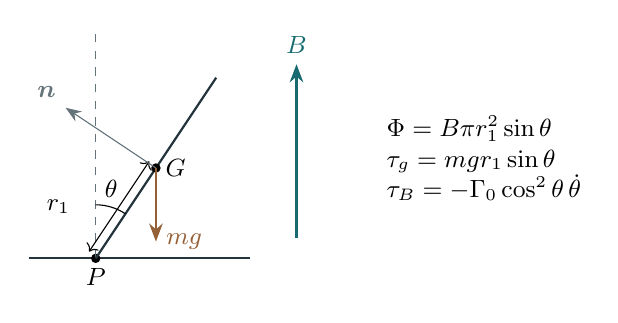
\begin{tikzpicture}[scale=.85]

\draw[object] (-1,0)--(2.3,0);\fill (0,0) circle(2pt) node[below]{$P$};
\draw[guide] (0,0)--(0,3.4);\draw[object] (0,0)--(1.8,2.7);
\fill (.9,1.35) circle(2pt) node[right]{$G$};\draw[force] (.9,1.35)--(.9,.25) node[right]{$mg$};
\draw[<->] (-.1,.1)--(.8,1.45) node[midway,left,xshift=-5mm]{$r_1$};
\draw (0,.8) arc(90:56.3:.8) node[midway,above]{$\theta$};
\draw[motion] (3,.3)--(3,2.9) node[above]{$B$};
\draw[axis] (.9,1.35)--(-.45,2.25) node[above left]{$\vect n$};
\node[align=left] at(5.8,1.5){$\Phi=B\pi r_1^2\sin\theta$\\$\tau_g=mg r_1\sin\theta$\\$\tau_B=-\Gamma_0\cos^2\theta\,\dot\theta$};

\end{tikzpicture}\figcaption{解图电3.3A\quad 法线投影决定磁通，重心横移决定重力矩。}\end{minipage}\end{center}

环面磁通量为$\Phi=B\pi r_1^2\sin\theta$，因此感应电流大小为
\[
I=\frac{B\pi r_1^2}{R_e}\cos\theta\,\dot\theta.
\]
磁矩与$B$的夹角使磁阻力矩为
\[
M_B=I\pi r_1^2B\cos\theta
=\Gamma_0\cos^2\theta\,\dot\theta,
\qquad \Gamma_0=\frac{B^2\pi^2r_1^4}{R_e}.
\]
它阻碍倾倒，重力矩为$M_g=mg r_1\sin\theta$。完整运动与能量方程是
\[
J\ddot\theta=mg r_1\sin\theta-\Gamma_0\cos^2\theta\,\dot\theta,
\qquad \theta(0)=\theta_0,\quad\dot\theta(0)=0,
\]
\[
\frac{\dd}{\dd t}\left(\frac12J\dot\theta^2+mg r_1\cos\theta\right)
=-\Gamma_0\cos^2\theta\,\dot\theta^2=-I^2R_e.
\]
故到水平位置时，严格的能量关系为
\[
\boxed{mg r_1\cos\theta_0=Q+\frac12J\omega_f^2}.
\]
判断耗散强弱可比较重力运动时间$t_g=\sqrt{J/(mg r_1)}$与阻尼参数$K=\Gamma_0/(mg r_1)$：
\[
t_g\simeq0.0391\,\mathrm s,\qquad
K=\frac{\sigma B^2r_1}{4\rho g}\simeq1.785\,\mathrm s.
\]
$K/t_g\simeq45.6$。在 $\cos^2\theta$ 仍较大的角区，磁阻尼使运动缓慢。接近水平位置时，解图电3.3B的 $\cos^2\theta$ 迅速趋零，重力矩却接近 $mg r_1$，于是圆环最后一段加速。末动能由此时的瞬时角速度 $\omega_f$ 给出。

\begin{center}\begin{minipage}{.98\linewidth}\centering
\begin{tikzpicture}[scale=.85]

\draw[axis] (0,0)--(5.5,0) node[right]{$\theta$};\draw[axis] (0,0)--(0,2.7) node[above]{$\Gamma/\Gamma_0$};
\draw[traj,domain=0:90,samples=70] plot ({\x/20},{2*cos(\x)^2});
\node[left] at(0,2){$1$};\node[below] at(4.5,0){$\pi/2$};
\node[align=left] at(7.6,1.3){$\Gamma=\Gamma_0\cos^2\theta$\\临近水平时阻尼衰减\\末段重力矩仍接近最大值};

\end{tikzpicture}\figcaption{解图电3.3B\quad 阻尼系数随倾角下降，在水平位置降为零。}\end{minipage}\end{center}

例如按上述完整初值方程作数值积分，题给$\theta_0=1.0\,\mathrm{rad}$时，倾倒时间约$0.141\,\mathrm s$，$\omega_f\simeq16.16\,\mathrm{rad/s}$，从而
\[
\frac{\tfrac12J\omega_f^2}{mg r_1\cos\theta_0}\simeq0.370,
\qquad \frac{Q}{mg r_1\cos\theta_0}\simeq0.630.
\]
在这个初始角下，重力释放的能量多数成为焦耳热，其余成为末态动能。初始角改为 $0.10\,\mathrm{rad}$ 时，用到达末态的瞬时转速计算，末态动能占比仍约为 $0.201$。

\begin{center}\begin{minipage}{.97\linewidth}\centering
\begin{tikzpicture}[x=5cm,y=3cm,font=\small]
\draw[axis] (0,0)--(1.12,0) node[right] {$u$};\draw[axis] (0,0)--(0,.85) node[above] {能量$/\Delta U_g$};
\draw[traj] plot coordinates {(0.000000,0.000000) (0.003047,0.001477) (0.009435,0.002807) (0.017126,0.003478) (0.025389,0.003831) (0.033965,0.004062) (0.042761,0.004251) (0.051748,0.004431) (0.060922,0.004615) (0.070284,0.004808) (0.079841,0.005013) (0.089603,0.005232) (0.099580,0.005468) (0.109782,0.005722) (0.120221,0.005996) (0.130911,0.006292) (0.141867,0.006613) (0.153103,0.006962) (0.164637,0.007342) (0.176487,0.007758) (0.188675,0.008215) (0.201223,0.008717) (0.214156,0.009271) (0.227503,0.009886) (0.241294,0.010570) (0.255564,0.011334) (0.270353,0.012193) (0.285705,0.013162) (0.301671,0.014261) (0.318307,0.015517) (0.335679,0.016958) (0.353863,0.018626) (0.372945,0.020568) (0.393027,0.022850) (0.414229,0.025554) (0.436691,0.028787) (0.460580,0.032694) (0.486095,0.037468) (0.513478,0.043371) (0.543021,0.050763) (0.575079,0.060145) (0.610091,0.072217) (0.648595,0.087968) (0.691254,0.108784) (0.738876,0.136579) (0.792432,0.173891) (0.853038,0.223767) (0.921881,0.289027) (1.000000,0.370086)};
\draw[thick,warm] plot coordinates {(0.000000,0.000000) (0.003047,0.001233) (0.009435,0.005595) (0.017126,0.011794) (0.025389,0.018844) (0.033965,0.026318) (0.042761,0.034056) (0.051748,0.042001) (0.060922,0.050136) (0.070284,0.058460) (0.079841,0.066977) (0.089603,0.075694) (0.099580,0.084622) (0.109782,0.093769) (0.120221,0.103146) (0.130911,0.112766) (0.141867,0.122641) (0.153103,0.132784) (0.164637,0.143211) (0.176487,0.153937) (0.188675,0.164980) (0.201223,0.176359) (0.214156,0.188094) (0.227503,0.200207) (0.241294,0.212723) (0.255564,0.225669) (0.270353,0.239072) (0.285705,0.252963) (0.301671,0.267378) (0.318307,0.282352) (0.335679,0.297926) (0.353863,0.314140) (0.372945,0.331040) (0.393027,0.348672) (0.414229,0.367081) (0.436691,0.386313) (0.460580,0.406403) (0.486095,0.427375) (0.513478,0.449229) (0.543021,0.471922) (0.575079,0.495341) (0.610091,0.519260) (0.648595,0.543278) (0.691254,0.566731) (0.738876,0.588580) (0.792432,0.607339) (0.853038,0.621159) (0.921881,0.628473) (1.000000,0.629914)};
\node[right,warm] at (1.08,.64) {$Q/\Delta U_g\simeq0.630$};
\node[right,accent] at (1.08,.37) {$K_{\rm rot}/\Delta U_g\simeq0.370$};
\node[below] at (1,0) {$1$};\node[below] at (.5,-.23) {$u=(\theta-\theta_0)/(\pi/2-\theta_0)$};
\end{tikzpicture}
\figcaption{解图电3.3C　题给$\theta_0=1.0$的完整初值方程数值解。横轴按已经倾倒的角度归一化；热量曲线对瞬时耗散率积分得到，动能曲线取每个倾角处的瞬时角速度。}
\end{minipage}\end{center}

\textbf{准静态时间。}第二问明确略去$J\ddot\theta$，于是
\[
\Gamma_0\cos^2\theta\,\dot\theta=mg r_1\sin\theta,
\qquad \dd t=K\frac{\cos^2\theta}{\sin\theta}\dd\theta.
\]
将被积函数写成$\csc\theta-\sin\theta$，逐项积分：
\[
T_{\rm qs}=K\int_{\theta_0}^{\pi/2}\frac{\cos^2\theta}{\sin\theta}\dd\theta
=K\left[\ln\tan\frac\theta2+\cos\theta\right]_{\theta_0}^{\pi/2},
\]
\[
\boxed{T_{\rm qs}=\frac{\sigma B^2r_1}{4\rho g}
\left[-\ln\tan\frac{\theta_0}{2}-\cos\theta_0\right]}.
\]
取$\theta_0=1.0\,\mathrm{rad}$得$T_{\rm qs}\simeq0.115\,\mathrm s$；取$0.10\,\mathrm{rad}$则得$3.57\,\mathrm s$。两个初始角到水平的余下转角不同，且阻尼最大的角区接近竖直。准静态式适用于角加速度相对较小的中段。释放后的短暂调整阶段与水平位置附近均需保留惯性项，最后的角速度由初值方程给出。

准静态近似的误差还可在角度上作估计。令$\omega_{\rm qs}=\sin\theta/(K\cos^2\theta)$，沿这一近似轨迹求导，得到
\[
\ddot\theta_{\rm qs}=\omega_{\rm qs}\frac{\dd\omega_{\rm qs}}{\dd\theta}
=\frac{\sin\theta(1+\sin^2\theta)}{K^2\cos^5\theta},
\]
\[
\epsilon_{\rm in}=\frac{J|\ddot\theta_{\rm qs}|}{mg r_1\sin\theta}
=\left(\frac{t_g}{K}\right)^2\frac{1+\sin^2\theta}{\cos^5\theta}.
\]
当 $\epsilon_{\rm in}\ll1$ 时，准静态轨迹上所需的惯性力矩远小于重力矩，磁阻力矩和重力矩近似平衡。对本题参数，在$\theta=1.0$处该比值约为$0.018$，但临近水平时按$\cos^{-5}\theta$增长。取终端$1+\sin^2\theta\simeq2$估计，$\epsilon_{\rm in}\sim1$约发生在$\pi/2-\theta\sim[2(t_g/K)^2]^{1/5}\simeq0.25\,\mathrm{rad}$。进入这一角区后，角加速度与重力矩同阶贡献。释放瞬间又有$\dot\theta=0$，也需经历建立阻尼速度的短暂调整。这个角度判据与解图电3.3B的阻尼趋零相对应。


\textbf{平均电流与总热量。} 解图电3.3C取$\Delta U_g=mgr_1\cos\theta_0$，从释放点逐步积分瞬时热功率。
平均电流满足$\overline I\,T=|\Delta\Phi|/R_e$，但焦耳热为$R_eT\overline{I^2}$；
用 $\overline{I^2}\ge\overline I^2$ 可得
\[
Q\ge\frac{B^2\pi^2r_1^4(1-\sin\theta_0)^2}{R_eT}.
\]
热量比下界多出的部分为 $R_e\int_0^T(I-\overline I)^2\dd t$。转动平均角速度 $(\pi/2-\theta_0)/T$ 给总转角与历时的比。重力在最后的弱阻尼区仍做正功，角速度持续上升，解图电3.3C中的末动能取最后时刻的 $\omega_f$。

按图A的力矩方向积分，采用状态$\theta,\omega,Q$，并单独加入$\dot Q=\Gamma_0\cos^2\theta\,\omega^2$，
以到达 $\theta=\pi/2$ 为停止事件，从最后的状态读取转速和热量。题给参数得到 $T\simeq0.14066\,\mathrm s$、$\omega_f\simeq16.1641\,\mathrm{rad/s}$。解图电3.3C显示，在最后几个转角内热量曲线接近水平，重力势能损失主要进入转动动能。第二问将中段的准静态积分延伸至水平，得到形式时间 $T_{\rm qs}\simeq0.115\,\mathrm s$。

第二问积分还可写成
\[
T_{\rm qs}=K\left[-\cos\theta_0+\frac12\ln\frac{1+\cos\theta_0}{1-\cos\theta_0}\right],
\]
因$-\ln\tan(\theta_0/2)=\tfrac12\ln[(1+\cos\theta_0)/(1-\cos\theta_0)]$，与前式严格相同。
这个形式直接用初始高度的无量纲比值 $\cos\theta_0$ 来算。当 $\theta_0$ 减小时，分母 $1-\cos\theta_0$ 与 $\theta_0^2/2$ 同阶，因而用时会按初始角的对数增长。


\Needspace{8\baselineskip}

\pdfbookmark[3]{关键洞察}{q3-h5}

\subsection*{关键洞察}

$K/t_g$ 衡量磁阻尼参数与重力转动时间的相对大小，实际阻尼还含角度因子。终点磁通对倾角的一阶导数为零，此处电流趋零，而角速度仍有限。磁阻尼最强的角区对历时影响大，弱阻尼的末段则积累了相当一部分转动动能。

\Needspace{8\baselineskip}

\pdfbookmark[3]{易错点}{q3-h6}

\subsection*{易错点}

\begin{itemize}
\item 初始倾角为 $1.0\,\mathrm{rad}$，初始重力势能相对水平为 $mg r_1\cos(1.0)$。
\item 放手时 $\dot\theta(0)=0$，重力矩给初角加速度 $\sin\theta_0/t_g^2$。环先从静止起动，再接近解图中重力矩与磁阻尼矩平衡的准静态曲线；该曲线在 $\theta_0$ 的外推值为 $\sin\theta_0/(K\cos^2\theta_0)$。
\item $\overline I$ 由磁通端点差得到，发热量使用电流的均方。末态动能使用 $\omega_f$。
\end{itemize}

\Needspace{8\baselineskip}

\pdfbookmark[3]{课堂讲解建议}{q3-h7}

\subsection*{课堂讲解建议}

用解图电3.3A让学生分别标出重力矩、磁阻力矩的两个角度关系，再问靠近水平时哪一个力矩先趋零。两组学生可分别计算初值方程和准静态时间，用解图电3.3C追问为何末动能约占总势能差的 $0.370$。把初角改成 $0.10$ 弧度，结合变图电3.3V2的对数增长，说明多出的时间集中在哪些角区。最后请学生在变图电3.3V6的热功率曲线下指出累计热量对应的面积。

\Needspace{18\baselineskip}
\pdfbookmark[3]{变式训练}{q3-h8}

\subsection*{变式训练}

\begin{enumerate}
\item 导线截面半径减半。变图电3.3V1左侧的实、虚圆分别代表两种截面，面积比为 $1:4$。由质量和电阻的表达式，$m,J,\Gamma_0$ 均缩为原先的四分之一，$R_e$ 增为四倍。将运动方程除以 $mg r_1$，$t_g^2$ 和 $K$ 均保持，初始倾角与速度相同，右侧两条运动曲线重合。准静态时间不变，热量和转动动能均缩为四分之一。
\begin{center}\begin{minipage}{.98\linewidth}\centering
\begin{tikzpicture}[scale=.85,transform shape]
\draw[object](-.5,0)--(0,0);
\draw[object](0,0)circle(1.43);
\draw[guide](0,0)circle(.715);
\draw[<->](0,-.14)--(1.43,-.14)node[midway,below]{$r_2$};
\draw[axis](2.52,0)--(6.65,0)node[right]{$t/T$};
\draw[axis](2.52,0)--(2.52,2.5)node[above]{$\theta$};
\draw[traj]plot coordinates {(2.520000,0.380000) (2.582698,0.383180) (2.645397,0.390335) (2.708095,0.399396) (2.770794,0.409416) (2.833492,0.419962) (2.896190,0.430836) (2.958889,0.441949) (3.021587,0.453262) (3.084286,0.464761) (3.146984,0.476440) (3.209683,0.488302) (3.272381,0.500350) (3.335079,0.512589) (3.397778,0.525027) (3.460476,0.537671) (3.523175,0.550529) (3.585873,0.563608) (3.648571,0.576918) (3.711270,0.590470) (3.773968,0.604272) (3.836667,0.618336) (3.899365,0.632674) (3.962063,0.647298) (4.024762,0.662222) (4.087460,0.677461) (4.150159,0.693029) (4.212857,0.708944) (4.275556,0.725223) (4.338254,0.741887) (4.400952,0.758957) (4.463651,0.776455) (4.526349,0.794408) (4.589048,0.812842) (4.651746,0.831788) (4.714444,0.851278) (4.777143,0.871349) (4.839841,0.892041) (4.902540,0.913398) (4.965238,0.935469) (5.027937,0.958309) (5.090635,0.981979) (5.153333,1.006547) (5.216032,1.032090) (5.278730,1.058695) (5.341429,1.086459) (5.404127,1.115495) (5.466825,1.145930) (5.529524,1.177910) (5.592222,1.211603) (5.654921,1.247205) (5.717619,1.284941) (5.780317,1.325073) (5.843016,1.367910) (5.905714,1.413811) (5.968413,1.463198) (6.031111,1.516564) (6.093810,1.574485) (6.156508,1.637627) (6.219206,1.706748) (6.281905,1.782688) (6.344603,1.866333) (6.407302,1.958543) (6.470000,2.060000)};
\node[below]at(6.47,0){$1$};
\node[left]at(2.52,.38){$\theta_0$};\node[left]at(2.52,2.06){$\pi/2$};
\node[align=left]at(4.6,2.6){两种截面共用同一角度轨迹};
\end{tikzpicture}
\figcaption{变图电3.3V1\quad 缩小导线截面后，薄环的倾角随时间仍沿同一曲线}
\end{minipage}\end{center}
\item 令初始角 $\theta_0$ 趋零。$\tan(\theta_0/2)=\theta_0/2+O(\theta_0^3)$、$\cos\theta_0=1+O(\theta_0^2)$，所以
\[T_{\rm qs}/K=\ln(2/\theta_0)-1+O(\theta_0^2).\]
变图电3.3V2的横坐标是 $\ln(2/\theta_0)$，小初角时实线趋近虚直线，反映竖直附近用时的对数增长。若恰从 $\theta_0=0,\dot\theta_0=0$ 释放，完整方程右端为零，竖直静止是初值解。
\begin{center}\begin{minipage}{.98\linewidth}\centering
\begin{tikzpicture}[scale=.85,transform shape]
\draw[axis](0,.45)--(5.2,.45)node[right]{$\ln(2/\theta_0)$};
\draw[axis](0,.45)--(0,2.65)node[above]{$T_{\rm qs}/K$};
\draw[object,dashed](.15,.45)--(4.75,2.52);
\draw[traj,domain=1.12:5.2,samples=63,variable=\u]plot({\u-.85},{.45*(-ln(tan(exp(-\u)*180/pi))-cos(2*exp(-\u)*180/pi))+.45});
\node[above left]at(3.65,2.12){$T_{\rm qs}/K$};
\node[below right]at(3.3,1.52){斜率为 $1$};
\node[below]at(0,.45){$0.85$};
\node[left]at(0,.45){$0$};\node[left]at(0,.90){$1$};\node[left]at(0,1.35){$2$};
\end{tikzpicture}
\figcaption{变图电3.3V2\quad 初角越小，释放点在对数坐标上越向右}
\end{minipage}\end{center}
\item 将 $B$ 减半。因 $\Gamma_0\propto B^2$，阻尼时间参数 $K$ 变为四分之一；$t_g$ 仍只由升降的机械尺度给出。代入 $\epsilon_{\rm in}=(t_g/K)^2(1+\sin^2\theta)/\cos^5\theta$，同一倾角的数值增为16倍。变图电3.3V3的虚线比实线更早达到水平参考线 $\epsilon_{\rm in}=1$，表示可用力矩平衡的角区缩小。
\begin{center}\begin{minipage}{.98\linewidth}\centering
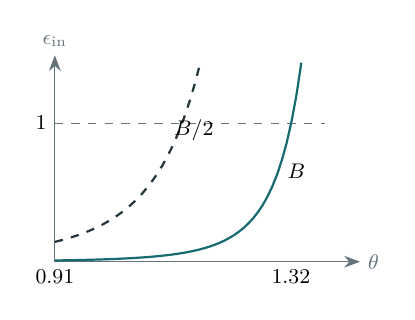
\begin{tikzpicture}[scale=.85,transform shape]
\begin{scope}[x=8.6cm,y=2.07cm]
\draw[axis](0,0)--(.53,0)node[right]{$\theta$};
\draw[axis](0,0)--(0,1.49)node[above]{$\epsilon_{\rm in}$};
\draw[guide](0,1)--(.47,1);\node[left]at(0,1){$1$};
\draw[traj]plot coordinates {(0.000000,0.008950) (0.008396,0.009499) (0.016792,0.010090) (0.025189,0.010728) (0.033585,0.011417) (0.041981,0.012162) (0.050377,0.012969) (0.058774,0.013843) (0.067170,0.014792) (0.075566,0.015823) (0.083962,0.016944) (0.092358,0.018165) (0.100755,0.019497) (0.109151,0.020952) (0.117547,0.022543) (0.125943,0.024285) (0.134340,0.026196) (0.142736,0.028295) (0.151132,0.030605) (0.159528,0.033150) (0.167925,0.035960) (0.176321,0.039067) (0.184717,0.042509) (0.193113,0.046330) (0.201509,0.050578) (0.209906,0.055311) (0.218302,0.060596) (0.226698,0.066510) (0.235094,0.073141) (0.243491,0.080596) (0.251887,0.088995) (0.260283,0.098483) (0.268679,0.109229) (0.277075,0.121432) (0.285472,0.135329) (0.293868,0.151204) (0.302264,0.169393) (0.310660,0.190303) (0.319057,0.214420) (0.327453,0.242338) (0.335849,0.274776) (0.344245,0.312615) (0.352642,0.356937) (0.361038,0.409082) (0.369434,0.470712) (0.377830,0.543910) (0.386226,0.631298) (0.394623,0.736200) (0.403019,0.862861) (0.411415,1.016748) (0.419811,1.204955) (0.428208,1.436771)};
\draw[object,dashed]plot coordinates {(0.000000,0.143206) (0.008108,0.151668) (0.016216,0.160765) (0.024324,0.170557) (0.032432,0.181104) (0.040541,0.192478) (0.048649,0.204756) (0.056757,0.218024) (0.064865,0.232377) (0.072973,0.247922) (0.081081,0.264776) (0.089189,0.283071) (0.097297,0.302956) (0.105405,0.324594) (0.113514,0.348171) (0.121622,0.373896) (0.129730,0.402000) (0.137838,0.432749) (0.145946,0.466438) (0.154054,0.503406) (0.162162,0.544032) (0.170270,0.588750) (0.178378,0.638053) (0.186486,0.692503) (0.194595,0.752742) (0.202703,0.819508) (0.210811,0.893646) (0.218919,0.976129) (0.227027,1.068083) (0.235135,1.170808) (0.243243,1.285814) (0.251351,1.414860)};
\node[below]at(0,0){$0.91$};\node[below]at(.41,0){$1.32$};
\node[right]at(.39,.65){$B$};\node[left]at(.29,.95){$B/2$};
\end{scope}
\end{tikzpicture}
\figcaption{变图电3.3V3\quad 磁场减半使惯性相对量更早接近1}
\end{minipage}\end{center}
\item 求中途从 $\theta_a$ 到 $\theta_b$ 的准静态时间。只在两端之间积分，
\[T_{ab}=K[\ln\tan(\theta/2)+\cos\theta]_{\theta_a}^{\theta_b}.\]
变图电3.3V4的阴影以 $2\theta/\pi$ 为横轴，因此面积乘 $K\pi/2$ 才给实际时间。若到 $\theta_a$ 时圆环已进入近似平衡段，可用 $\epsilon_{\rm in}(\theta_b)\ll1$ 给出此区间的惯性条件，因为它在 $0<\theta<\pi/2$ 随角度增大。
\begin{center}\begin{minipage}{.98\linewidth}\centering
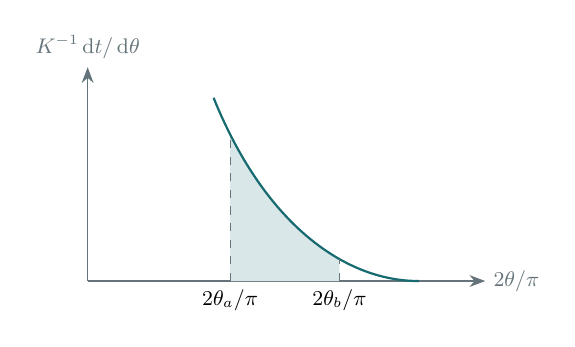
\begin{tikzpicture}[scale=.85,transform shape]
\begin{scope}[x=4.95cm,y=2.25cm]
\draw[axis](0,0)--(1.2,0)node[right]{$2\theta/\pi$};
\draw[axis](0,0)--(0,1.42)node[above]{$K^{-1}\dd t/\dd\theta$};
\fill[accent!16](.43,0)--plot[domain=.43:.76,samples=56](\x,{cos(90*\x)^2/sin(90*\x)})--(.76,0)--cycle;
\draw[traj,domain=.38:1,samples=75]plot(\x,{cos(90*\x)^2/sin(90*\x)});
\draw[guide](.43,0)--(.43,{cos(90*.43)^2/sin(90*.43)})(.76,0)--(.76,{cos(90*.76)^2/sin(90*.76)});
\node[below]at(.43,0){$2\theta_a/\pi$};\node[below]at(.76,0){$2\theta_b/\pi$};
\end{scope}
\end{tikzpicture}
\figcaption{变图电3.3V4\quad 两倾角之间的准静态时间由着色面积给出}
\end{minipage}\end{center}
\item 用 $\lambda=t_g/K$ 估计水平附近的惯性角宽。令 $\delta=\pi/2-\theta$，近终点 $\cos\theta\simeq\delta$ 且 $1+\sin^2\theta\simeq2$，所以 $\epsilon_{\rm in}\simeq2\lambda^2/\delta^5$。取 $\epsilon_{\rm in}=1$ 定义过渡尺度，得 $\delta_{\rm end}\sim(2\lambda^2)^{1/5}\simeq0.25\,\mathrm{rad}$。变图电3.3V5以这个尺度归一化角差，从右向左接近水平时，曲线迅速升过1。
\begin{center}\begin{minipage}{.98\linewidth}\centering
\begin{tikzpicture}[scale=.85,transform shape]
\begin{scope}[x=5.2cm,y=2.3cm]
\draw[axis](0,0)--(1.15,0)node[right]{$\delta/\delta_{\rm end}$};
\draw[axis](0,0)--(0,1.5)node[above]{$\epsilon_{\rm in}$};
\fill[accent!13](0,0)rectangle(.5,1.35);
\draw[guide](0,1)--(.5,1)--(.5,0);
\draw[traj,domain=.465:1.02,samples=66]plot(\x,{(.5/\x)^5});
\node[above left]at(.25,.85){惯性影响较大};
\node[below]at(.5,0){$1$};\node[below]at(1,0){$2$};
\node[left]at(0,1){$1$};
\end{scope}
\end{tikzpicture}
\figcaption{变图电3.3V5\quad 末段近似中，离水平的角差按五次幂影响惯性比值}
\end{minipage}\end{center}
\item 对解图电3.3C数值积分中的机械能与热量分别取值。除 $\theta,\omega$ 的方程外，单独积分 $\dot Q=\Gamma_0\cos^2\theta\,\omega^2$，初值为 $Q=0$。变图电3.3V6以 $t/T$ 为横轴，因此纵轴乘了 $T/\Delta U_g$，面积给 $Q/\Delta U_g$。各时刻把三个独立积分得到的量代入 $\frac12J\omega^2+mg r_1\cos\theta+Q$，所得值应接近初始势能。减小积分容差，可比较三个状态的末值。
\begin{center}\begin{minipage}{.98\linewidth}\centering
\begin{tikzpicture}[scale=.85,transform shape]
\begin{scope}[x=5.9cm,y=2.75cm]
\draw[axis](0,0)--(1.15,0)node[right]{$t/T$};
\draw[axis](0,0)--(0,1.31)node[above]{$T\dot Q/\Delta U_g$};
\fill[accent!18](0,0)--plot coordinates {(0.000000,0.000000) (0.015873,0.100122) (0.031746,0.215703) (0.047619,0.286160) (0.063492,0.324855) (0.079365,0.346618) (0.095238,0.360105) (0.111111,0.369707) (0.126984,0.377558) (0.142857,0.384678) (0.158730,0.391560) (0.174603,0.398444) (0.190476,0.405453) (0.206349,0.412651) (0.222222,0.420077) (0.238095,0.427759) (0.253968,0.435717) (0.269841,0.443970) (0.285714,0.452537) (0.301587,0.461437) (0.317460,0.470690) (0.333333,0.480317) (0.349206,0.490340) (0.365079,0.500785) (0.380952,0.511677) (0.396825,0.523045) (0.412698,0.534918) (0.428571,0.547330) (0.444444,0.560316) (0.460317,0.573913) (0.476190,0.588161) (0.492063,0.603105) (0.507937,0.618791) (0.523810,0.635268) (0.539683,0.652589) (0.555556,0.670808) (0.571429,0.689984) (0.587302,0.710176) (0.603175,0.731444) (0.619048,0.753848) (0.634921,0.777443) (0.650794,0.802278) (0.666667,0.828391) (0.682540,0.855799) (0.698413,0.884490) (0.714286,0.914406) (0.730159,0.945422) (0.746032,0.977316) (0.761905,1.009726) (0.777778,1.042084) (0.793651,1.073539) (0.809524,1.102829) (0.825397,1.128122) (0.841270,1.146801) (0.857143,1.155183) (0.873016,1.148201) (0.888889,1.119096) (0.904762,1.059293) (0.920635,0.958876) (0.936508,0.808489) (0.952381,0.604301) (0.968254,0.358670) (0.984127,0.119656) (1.000000,0.000000)}--(1,0)--cycle;
\draw[traj]plot coordinates {(0.000000,0.000000) (0.015873,0.100122) (0.031746,0.215703) (0.047619,0.286160) (0.063492,0.324855) (0.079365,0.346618) (0.095238,0.360105) (0.111111,0.369707) (0.126984,0.377558) (0.142857,0.384678) (0.158730,0.391560) (0.174603,0.398444) (0.190476,0.405453) (0.206349,0.412651) (0.222222,0.420077) (0.238095,0.427759) (0.253968,0.435717) (0.269841,0.443970) (0.285714,0.452537) (0.301587,0.461437) (0.317460,0.470690) (0.333333,0.480317) (0.349206,0.490340) (0.365079,0.500785) (0.380952,0.511677) (0.396825,0.523045) (0.412698,0.534918) (0.428571,0.547330) (0.444444,0.560316) (0.460317,0.573913) (0.476190,0.588161) (0.492063,0.603105) (0.507937,0.618791) (0.523810,0.635268) (0.539683,0.652589) (0.555556,0.670808) (0.571429,0.689984) (0.587302,0.710176) (0.603175,0.731444) (0.619048,0.753848) (0.634921,0.777443) (0.650794,0.802278) (0.666667,0.828391) (0.682540,0.855799) (0.698413,0.884490) (0.714286,0.914406) (0.730159,0.945422) (0.746032,0.977316) (0.761905,1.009726) (0.777778,1.042084) (0.793651,1.073539) (0.809524,1.102829) (0.825397,1.128122) (0.841270,1.146801) (0.857143,1.155183) (0.873016,1.148201) (0.888889,1.119096) (0.904762,1.059293) (0.920635,0.958876) (0.936508,0.808489) (0.952381,0.604301) (0.968254,0.358670) (0.984127,0.119656) (1.000000,0.000000)};
\node[above]at(.52,.51){面积 $Q/\Delta U_g$};
\node[below]at(1,0){$1$};\node[left]at(0,1){$1$};
\end{scope}
\end{tikzpicture}
\figcaption{变图电3.3V6\quad 直接积累热功率获得解图电3.3C的终态热量}
\end{minipage}\end{center}
\item 比较完整方程与准静态式的终点电流。令 $C=B\pi r_1^2/R_e$，则 $I=C\cos\theta\,\omega$。近似平衡给 $\omega=\sin\theta/(K\cos^2\theta)$，所以 $I_{\rm qs}=(C/K)\tan\theta$。变图电3.3V7取 $u=(\theta-\theta_0)/(\pi/2-\theta_0)$，虚线在向 $u=1$ 延伸时发散，正是因为此时准静态角速度含 $1/\cos^2\theta$。实线由完整方程作出，$\omega_f$ 有限，乘以 $\cos\theta$ 后电流趋零。
\begin{center}\begin{minipage}{.98\linewidth}\centering
\begin{tikzpicture}[scale=.85,transform shape]
\begin{scope}[x=6.3cm,y=.57cm]
\draw[axis](0,0)--(1.13,0)node[right]{$u$};
\draw[axis](0,0)--(0,7.18)node[above]{$I/(C/K)$};
\draw[traj]plot coordinates {(0.000000,0.000000) (0.001893,0.828639) (0.006152,1.216265) (0.011545,1.400890) (0.017510,1.492604) (0.023787,1.541792) (0.030259,1.571500) (0.036874,1.592315) (0.043609,1.609132) (0.050453,1.624234) (0.057405,1.638699) (0.064465,1.653042) (0.071637,1.667516) (0.078922,1.682253) (0.086326,1.697323) (0.093852,1.712772) (0.101505,1.728630) (0.109290,1.744925) (0.117213,1.761680) (0.125280,1.778919) (0.133495,1.796666) (0.141867,1.814947) (0.150401,1.833787) (0.159106,1.853214) (0.167990,1.873260) (0.177060,1.893954) (0.186327,1.915330) (0.195800,1.937424) (0.205490,1.960272) (0.215409,1.983914) (0.225569,2.008391) (0.235985,2.033745) (0.246671,2.060023) (0.257644,2.087269) (0.268921,2.115533) (0.280522,2.144861) (0.292470,2.175302) (0.304786,2.206902) (0.317499,2.239704) (0.330636,2.273745) (0.344232,2.309054) (0.358321,2.345646) (0.372945,2.383514) (0.388149,2.422623) (0.403985,2.462898) (0.420511,2.504202) (0.437795,2.546319) (0.455911,2.588914) (0.474946,2.631490) (0.495002,2.673323) (0.516194,2.713369) (0.538655,2.750135) (0.562544,2.781493) (0.588042,2.804426) (0.615364,2.814656) (0.644761,2.806137) (0.676526,2.770343) (0.711003,2.695306) (0.748587,2.564374) (0.789731,2.354707) (0.834933,2.035761) (0.884722,1.568366) (0.939609,0.905874) (1.000000,0.000000)};
\draw[object,dashed,domain=0:.72,samples=57,variable=\u]plot(\u,{tan((1+(pi/2-1)*\u)*180/pi)});
\draw[guide](1,0)--(1,6.94);
\node[right]at(.71,6.17){力矩平衡式};
\node[above right]at(.58,1.94){完整方程};
\node[below]at(1,0){$1$};
\end{scope}
\end{tikzpicture}
\figcaption{变图电3.3V7\quad 水平位置的电流由有限的角速度乘以趋零的法向投影变化率}
\end{minipage}\end{center}
\item 仅改变主半径 $r_1$。由 $K=\sigma B^2r_1/(4\rho g)$、$t_g=\sqrt{3r_1/(2g)}$ 可得 $K\propto r_1$、$t_g\propto\sqrt{r_1}$，故 $K/t_g\propto\sqrt{r_1}$。变图电3.3V8把三项除以各自在参考主半径 $r_*$ 时的值。环越大，中段阻尼相对越强；由 $\delta_{\rm end}\sim[2(t_g/K)^2]^{1/5}$，末段惯性角宽约按 $r_1^{-1/5}$ 缩小。
\begin{center}\begin{minipage}{.98\linewidth}\centering
\begin{tikzpicture}[scale=.85,transform shape]
\begin{scope}[x=2.23cm,y=1.74cm]
\draw[axis](0,0)--(3.09,0)node[right]{$r_1/r_*$};
\draw[axis](0,0)--(0,2.13)node[above]{参数除以 $r_*$ 时的值};
\draw[traj,domain=0:1.95,samples=55]plot(\x,{\x});
\draw[object,dashed,domain=0:2.86,samples=84]plot(\x,{sqrt(\x)});
\draw[guide](1,0)--(1,1)--(0,1);
\node[above left]at(1.53,1.55){$K$};
\node[right]at(2.3,1.51){$t_g$ 与 $K/t_g$};
\node[below]at(1,0){$1$};\node[left]at(0,1){$1$};
\end{scope}
\end{tikzpicture}
\figcaption{变图电3.3V8\quad 主半径改变时的线性和平方根尺度}
\end{minipage}\end{center}
\end{enumerate}

\clearpage

\pdfbookmark[2]{第 4 题 翻转线圈测地磁场的分支判断}{q4}

\section*{第 4 题\quad 翻转线圈测地磁场的分支判断}\label{q:4}

水平桌面上有矩形线圈$abcd$，$ab=\ell_1$指向北方，$bc=\ell_2$沿东西方向，总电阻为$R$，面积$S=\ell_1\ell_2$。先绕南北方向的中心轴翻转$180^\circ$，使$ab$与$cd$交换位置，测得通过导线的净电量绝对值为$Q_1$。再固定南侧的$ad$边，将北侧边抬起$90^\circ$使线圈竖直；线圈从水平状态的向上法线转向南方，测得这次净电量绝对值为$Q_2$。地磁场的水平分量向北，竖直分量可向上或向下。忽略自感。
求地磁场大小的可能值及各分支的条件；说明还需记录什么信息才能消除歧义。净电量指$\int I\dd t$，不等同于累计电量$\int|I|\dd t$。

\begin{center}\begin{minipage}{.98\linewidth}\centering
\begin{tikzpicture}[scale=.85]

\draw[object] (0,0) node[below left]{$a$}--(0,2.5) node[above left]{$b$}--(4,2.5) node[above right]{$c$}--(4,0) node[below right]{$d$}--cycle;
\draw[axis] (5,0)--(5,2) node[above]{北};\draw[axis] (5,0)--(6.5,0) node[right]{东};
\draw[<->] (-.5,0)--(-.5,2.5) node[midway,left]{$\ell_1$};\draw[<->] (0,-.6)--(4,-.6) node[midway,below]{$\ell_2$};
\draw[guide] (2,-.2)--(2,2.9);\node at(2,4){先绕南北轴翻转$180^\circ$};
\draw[motion] (.5,2.8)--(.5,3.4);\node at(5.7,3.4){再抬北边};

\end{tikzpicture}\figcaption{图电3.4\quad 俯视矩形及两次操作，第二步固定南边$ad$。}\end{minipage}\end{center}

\Needspace{8\baselineskip}

\pdfbookmark[3]{题型定位}{q4-h0}

\subsection*{题型定位}

用翻转线圈反推地磁分量。第一次测量固定竖直分量的绝对值，第二次测量把它与水平分量组合；读数保留方向时可直接求两个分量。

\Needspace{8\baselineskip}

\pdfbookmark[3]{知识点}{q4-h1}

\subsection*{知识点}

$\Phi=S\vect B\cdot\vect n$。材料绕向确定法线，同一绕向用于两次操作。恒电阻、忽略自感时 $Rq=-\Delta\Phi$。净电量是对有向电流积分，累计电量则对电流绝对值积分。分支由 $B_H\ge0$ 限定。

\Needspace{8\baselineskip}

\pdfbookmark[3]{物理图像}{q4-h2}

\subsection*{物理图像}

解图电3.4A把第二步法线的初向与末向画在南北竖直平面。图B画法线连续转动，向下场使磁通在法线接近反场方向时达到极小值。图C把三支 $B_H$ 画在读数坐标上，小根随 $c/b$ 跨过1而从向下场转为向上场。

\Needspace{8\baselineskip}

\pdfbookmark[3]{解题入口}{q4-h3}

\subsection*{解题入口}

先把读数换成 $b=RQ_1/(2S)$、$c=RQ_2/S$。在 $B_z=-b$ 和 $B_z=b$ 两种情况下分别解 $|B_H+B_z|=c$，保留非负根。若给有向电量，则直接写 $Rq_1=-2SB_z$、$Rq_2=S(B_H+B_z)$。

\Needspace{18\baselineskip}
\pdfbookmark[3]{标准解法}{q4-h4}

\subsection*{标准解法}

解图电3.4A取向北为$+y$、向上为$+z$，写地磁场为
\[
\vect B=B_H\vect e_y+B_z\vect e_z,\qquad B_H\ge0.
\]
第一步翻转使有向面积法线反向，磁通变化的绝对值为$2S|B_z|$。由$R\int I\dd t=-\Delta\Phi$，得
\[
b\equiv|B_z|=\frac{RQ_1}{2S}.
\]

\begin{center}\begin{minipage}{.98\linewidth}\centering
\begin{tikzpicture}[scale=.85]

\draw[axis] (0,0)--(3,0) node[right]{北$\ (+y)$};\draw[axis] (0,0)--(0,2.8) node[above]{上$\ (+z)$};
\draw[motion] (0,0)--(0,2) node[left]{$\vect n_i$};\draw[motion] (0,0)--(-2,0) node[left]{$\vect n_f$};
\draw[force] (0,0)--(2,-1.4) node[right]{$\vect B=B_H\vect e_y-b\vect e_z$};
\draw[guide] (2,0)--(2,-1.4)--(0,-1.4);\node[below] at(1,0){$B_H$};\node[left] at(0,-1.1){$b$};
\node[align=left] at(6,1.4){第二步初法线：向上\\末法线：向南\\$\Delta\Phi=S(b-B_H)$};

\end{tikzpicture}\figcaption{解图电3.4A\quad 示出竖直场向下的分支；第二步的法线由上转向南。}\end{minipage}\end{center}

第二步开始时法线为$+\vect e_z$，最后为$-\vect e_y$，所以
\[
\Phi_i=SB_z,\quad\Phi_f=-SB_H,\quad
c\equiv\frac{RQ_2}{S}=|B_H+B_z|.
\]
两次读数分别确定 $|B_z|$ 和 $|B_H+B_z|$。下面令 $B_z$ 向上或向下，再由第二个绝对值方程求 $B_H$。

\textbf{竖直分量向下。}此时$B_z=-b$，有$|B_H-b|=c$，因此
\[
B_H=b+c\quad\hbox{或}\quad B_H=b-c\ (b\ge c).
\]
两种磁场大小为
\[
\boxed{B=\sqrt{b^2+(b+c)^2}},\qquad
\boxed{B=\sqrt{b^2+(b-c)^2}\quad(b\ge c)}.
\]
第一式对应水平分量不小于向下分量；第二式对应水平分量不大于向下分量。写成读数为
\[
B=\frac{R}{\sqrt2S}\sqrt{Q_1^2\pm2Q_1Q_2+2Q_2^2},
\]
其中负号要求$Q_1\ge2Q_2$。

\textbf{竖直分量向上。}此时$B_z=b$，有$B_H+b=c$，故
\[
\boxed{B_H=c-b,\quad
B=\sqrt{b^2+(c-b)^2}\quad(c\ge b)}.
\]
它的存在条件是$2Q_2\ge Q_1$。在$b=c$处，向下场的第二支与向上场的水平分量均为零；两种竖直方向给同一场强大小 $b$。

若$Q_1=0$，竖直分量为零，直接由第二次读数得$B=B_H=RQ_2/S$。一般情况下，由独立测量知道地磁场向上或向下，可以确定 $B_z$ 的符号；对向下场，还需要第二次净电量的有向符号，才能判断$B_H-b$的符号。此时 $q_2>0$ 对应 $B_H>b$，$q_2<0$ 对应 $B_H<b$。

\begin{center}\begin{minipage}{.98\linewidth}\centering
\begin{tikzpicture}[scale=.85]

\draw[axis] (0,0)--(3,0) node[right]{北};\draw[axis] (0,0)--(0,2.8) node[above]{上};
\draw[traj] (0,2) arc(90:180:2);\draw[motion] (0,0)--(-1.4,1.4) node[above left]{$\vect n(\alpha)$};
\draw (0,.7) arc(90:135:.7) node[midway,above]{$\alpha$};
\node[align=left] at(5.9,1.4){$\Phi=-S(b\cos\alpha+B_H\sin\alpha)$\\$|\Phi|$可先增后减\\净电量会发生抵消};

\end{tikzpicture}\figcaption{解图电3.4B\quad 向下场中的磁通先降后升，两个区间的电流方向相反。}\end{minipage}\end{center}

解图电3.4B还说明第二次操作的测量含义。若竖直场向下，抬起角为$\alpha$时
\[
\Phi(\alpha)=-S(b\cos\alpha+B_H\sin\alpha).
\]
磁通可能先减小后增大，电流随之反向。冲击式净电量读数仍由两个端点相减确定，累计电量则从磁通极小点处分段，各段分别取绝对值再相加。

若实验同时记录电流方向，就可以把两个绝对值还原为两个线性关系。规定导线正向始终跟随$a\to b\to c\to d\to a$的材料标号；第一步前这个方向的法线向下，翻转后向上。记相应的有向净电量为$q_1,q_2$，则
\[
Rq_1=-2SB_z,\qquad Rq_2=S(B_H+B_z),
\]
\[
B_z=-\frac{Rq_1}{2S},\qquad
B_H=\frac R S\left(q_2+\frac{q_1}{2}\right).
\]
两条有向方程给出唯一的 $B_z,B_H$，其中向北为 $B_H\ge0$。由平方和开方得到 $B=\sqrt{B_H^2+B_z^2}$。在解图电3.4A中，纯水平场与第一次翻转的水平积分面平行，所以 $q_1=0$。纯竖直场在第二次翻转的终态与线圈平面平行，故第二次的净电量大小为第一次的一半。

\begin{center}\begin{minipage}{.97\linewidth}\centering
\begin{tikzpicture}[x=2cm,y=1cm,font=\small]
\draw[axis] (0,0)--(2.25,0) node[right] {$c/b$};\draw[axis] (0,0)--(0,3.5) node[above] {$B_H/b$};
\draw[traj] (0,1)--(2,3);\draw[traj] (0,1)--(1,0);
\draw[thick,warm,dashed] (1,0)--(2,1);
\draw[guide] (1,0)--(1,3.2);\node[below] at (1,0) {$1$};\node[left] at (0,1) {$1$};
\node[right,accent] at (2.15,2.7) {$B_z=-b$，$B_H=b+c$};
\node[right,accent] at (2.15,2.1) {$B_z=-b$，$B_H=b-c$};
\node[right,warm] at (2.15,1.4) {$B_z=+b$，$B_H=c-b$};
\node[right] at (2.15,.6) {$b>0$；负的水平分量舍去};
\end{tikzpicture}
\figcaption{解图电3.4C　两个绝对值读数对应的全部非负水平分量。实线为向下场两支，虚线为向上场支；交于横轴的两种竖直场方向仍不同。}
\end{minipage}\end{center}

解图电3.4C把存在条件放在读数坐标中：$c<b$时仅有向下场，但仍有两个不同的水平分量；
$c>b$时向下场大根与向上场根同时存在；$c=b$时另有水平分量为零的极限。
若只问B的大小，两个小根的平方形式可以写成同一个根式，但对应的竖直方向仍须分别说明。
当$c=0$且$b>0$时，向下场两式重合为$B_H=b$，两支给同一场强大小。若 $b=c=0$，两个分量同时为零。

翻转携带材料标号，也携带回路正向。题图俯视$a\to b\to c\to d$的初法线向下，第一次翻转后向上；
随后固定南边抬起北边，法线从向上转至向南，正是图A、B所用的第二步法线。
依同一材料绕向，在两步中连续跟踪法线并记录两个有向电量。若整组实验改用反向绕行，两个 $q_i$ 同时换号，法线也一同反向，所得场分量保持。

对解图电3.4B中的向下场，取 $b,B_H>0$，
$\Phi'(\alpha)=S(b\sin\alpha-B_H\cos\alpha)$在$\tan\alpha=B_H/b$改变符号。
因此一次看似简单的竖起操作也会先后出现相反电流。把完整电流波形带符号积分，极小点前后的两段电量部分相消，余量仍为两个端点磁通之差乘 $-1/R$。


\Needspace{8\baselineskip}

\pdfbookmark[3]{关键洞察}{q4-h5}

\subsection*{关键洞察}

法线方向和电流参考方向成对变化。只报 $|q_1|,|q_2|$ 时，每个符号都可能对应一个不同的场，解图电3.4C给出实际允许的分支。即使在 $b=c$ 的水平分量零点，向上与向下的场仍是不同方向。

\Needspace{8\baselineskip}

\pdfbookmark[3]{易错点}{q4-h6}

\subsection*{易错点}

\begin{itemize}
\item 第二步终法线向南，终磁通为 $-SB_H$。
\item 磁通在中途达到极值时，累计电量分两段取绝对值，净电量直接取端点差。
\item 向下场小根要求 $b\ge c$，向上场要求 $c\ge b$。当 $c=0$ 时向下场两根重合。
\end{itemize}

\Needspace{8\baselineskip}

\pdfbookmark[3]{课堂讲解建议}{q4-h7}

\subsection*{课堂讲解建议}

先让学生在解图电3.4A标出纯水平场和纯竖直场各次操作的端点磁通。补上一般场后，在解图电3.4C上依次读 $c<b,c>b,c=b$ 的分支，并代入 $b=2,c=1$ 读出向下场的 $B_H=3$ 与 $B_H=1$。转到变图电3.4V2，问端点等高时两段电流各将什么符号记入净电量。再让学生在变图电3.4V5上找出哪一个额外端点能给带符号分量的乘积。

\Needspace{18\baselineskip}
\pdfbookmark[3]{变式训练}{q4-h8}

\subsection*{变式训练}

\begin{enumerate}
\item 已知 $B_z<0$ 且 $B_H>b$。变图电3.4V1中向北分量的长度超过向下分量，差值为 $B_H-b=c$。因此 $B_H=b+c$，有向净电量 $q_2=Sc/R>0$。两分量相互正交，$B=\sqrt{b^2+(b+c)^2}$。
\begin{center}\begin{minipage}{.98\linewidth}\centering
\begin{tikzpicture}[scale=.85,transform shape]
\draw[axis](-2.5,0)--(3.18,0)node[right]{北};
\draw[axis](0,-2.64)--(0,1.78)node[above]{上};
\draw[force](0,0)--(2.4,0)node[midway,above]{$B_H=b+c$};
\draw[force](0,0)--(0,-1.42)node[midway,left]{$b$};
\draw[guide](2.4,0)--(2.4,-1.42)--(0,-1.42);
\draw[motion](0,0)--(2.4,-1.42)node[right]{$\vect B$};
\draw[<->](1.42,-.45)--(2.4,-.45)node[midway,below]{$c$};
\end{tikzpicture}
\figcaption{变图电3.4V1\quad 水平分量超过向下分量时，差值为正}
\end{minipage}\end{center}
\item 向下场中 $Q_2=0$，所以 $B_H=b$。按变图电3.4V2，$\Phi(\alpha)=-Sb(\cos\alpha+\sin\alpha)$ 在 $\alpha=\pi/4$ 达到 $-\sqrt2 Sb$，两端均为 $-Sb$。前半段磁通减小，$q_+=Sb(\sqrt2-1)/R$；后半段磁通增加，$q_-=-q_+$。累计电量为 $|q_+|+|q_-|=2Sb(\sqrt2-1)/R$。
\begin{center}\begin{minipage}{.98\linewidth}\centering
\begin{tikzpicture}[scale=.85,transform shape]
\draw[axis](0,0)--(5.55,0)node[right]{$\alpha$};
\draw[axis](0,-2.28)--(0,.35)node[above]{$\Phi/(Sb)$};
\draw[traj,domain=0:90,samples=69]plot({\x/18},{-cos(\x)-1.00000*sin(\x)});
\draw[guide](0,-1)--(5,-1);
\draw[guide](2.50000,0)--(2.50000,-1.41421);
\fill[accent](0,-1)circle(1.4pt) (2.50000,-1.41421)circle(1.4pt) (5,-1.00000)circle(1.4pt);
\node[below]at(2.50000,0){$\alpha_*$};\node[below]at(5,0){$\pi/2$};
\node[left]at(0,-1){$-1$};
\node[below]at(2.50000,-1.46421){最小磁通};
\end{tikzpicture}
\figcaption{变图电3.4V2\quad 端点磁通相同，两段各输运非零电量}
\end{minipage}\end{center}
\item 向下场中求抬起时的累计电量。变图电3.4V3的最小点满足 $\Phi'(\alpha_*)=S[b\sin\alpha_*-B_H\cos\alpha_*]=0$，故 $\tan\alpha_*=B_H/b$，最小磁通为 $-SB$。从初端到最小点得到正电量 $S(B-b)/R$，从最小点到末端得到负电量 $-S(B-B_H)/R$。两段取绝对值求和为 $Q_{\rm abs}=S(2B-b-B_H)/R$。
\begin{center}\begin{minipage}{.98\linewidth}\centering
\begin{tikzpicture}[scale=.85,transform shape]
\draw[axis](0,0)--(5.55,0)node[right]{$\alpha$};
\draw[axis](0,-2.28)--(0,.35)node[above]{$\Phi/(Sb)$};
\draw[traj,domain=0:90,samples=69]plot({\x/18},{-cos(\x)-1.60000*sin(\x)});
\draw[guide](0,-1)--(5,-1);
\draw[guide](3.22192,0)--(3.22192,-1.88680);
\fill[accent](0,-1)circle(1.4pt) (3.22192,-1.88680)circle(1.4pt) (5,-1.60000)circle(1.4pt);
\node[below]at(3.22192,0){$\alpha_*$};\node[below]at(5,0){$\pi/2$};
\node[left]at(0,-1){$-1$};
\node[below]at(3.22192,-1.93680){最小磁通};
\end{tikzpicture}
\figcaption{变图电3.4V3\quad 从最小点分别比较两端，得到两个区间的累计电量}
\end{minipage}\end{center}
\item 保留自感。变图电3.4V4在操作完成时刻 $t_f$ 仍有电流 $I_f$。初始静止且电流为零，操作阶段的净电量满足 $Rq_{0f}=-\Delta\Phi-LI_f$。随后外磁通不变，$I(t)=I_f\exp[-R(t-t_f)/L]$，尾段面积为 $LI_f/R$。把这段也积入读数，得到 $Rq=-\Delta\Phi$。
\begin{center}\begin{minipage}{.98\linewidth}\centering
\begin{tikzpicture}[scale=.85,transform shape]
\draw[axis](0,0)--(6.7,0)node[right]{$t$};
\draw[axis](0,0)--(0,2.0)node[above]{$I$};
\draw[traj](.37,0)..controls(1.0,.38)and(1.3,1.35)..(2.85,1.59);
\fill[accent!17](2.85,0)--plot[domain=0:3.25,samples=71]({2.85+\x},{1.59*exp(-1.4*\x)})--(6.1,0)--cycle;
\draw[traj,domain=0:3.25,samples=71]plot({2.85+\x},{1.59*exp(-1.4*\x)});
\draw[guide](2.85,0)--(2.85,1.59);
\node[below]at(2.85,0){$t_f$};
\node[left]at(2.86,1.61){$I_f$};
\node[above right]at(3.89,.56){衰减电量};
\end{tikzpicture}
\figcaption{变图电3.4V4\quad 操作结束后，电流尾段仍计入净电量}
\end{minipage}\end{center}
\item 增加向另一侧竖起的第三次测量。变图电3.4V5两个终法线分别指南、指北，起始法线同为向上。令 $c_2=RQ_2/S,c_3=RQ_3/S$，有 $c_2=|B_H+B_z|$、$c_3=|B_H-B_z|$。平方后相加、相减分别得
\[ B_H^2=(c_2^2+c_3^2)/2-b^2,\qquad c_2^2-c_3^2=4B_HB_z. \]
取 $B_H$ 的非负根；当 $B_Hb>0$ 时平方差的符号给竖直方向，纯竖直场仍可记录任一次有向电量确定方向。
\begin{center}\begin{minipage}{.98\linewidth}\centering
\begin{tikzpicture}[scale=.85,transform shape]
\draw[axis](-3.1,0)--(3.18,0)node[right]{北};
\draw[axis](0,-.32)--(0,2.54)node[above]{上};
\draw[force](0,.09)--(0,1.9)node[right]{$+\vect e_z$};
\draw[force](-.07,0)--(-2.34,0)node[above]{$-\vect e_y$};
\draw[force](.07,0)--(2.34,0)node[above]{$+\vect e_y$};
\draw[motion](115:1.23)arc(115:170:1.23);
\draw[motion](65:1.23)arc(65:10:1.23);
\node[left]at(-1.16,1.25){第二次};
\node[right]at(1.16,1.25){第三次};
\end{tikzpicture}
\figcaption{变图电3.4V5\quad 两次向相反侧竖起，终法线指向相反}
\end{minipage}\end{center}
\item 把竖起的线圈沿同一路径放回。变图电3.4V6两段的端点磁通差互为相反数，所以 $q_{\rm back}=-q_2$。累计电量和焦耳热均由每段的非负量相加。若返程速度历程正好倒序，恒定 $R$ 下 $I_{\rm back}(t)=-I_{\rm out}(T-t)$，两段 $\int I^2R\dd t$ 相等。
\begin{center}\begin{minipage}{.98\linewidth}\centering
\begin{tikzpicture}[scale=.85,transform shape]
\draw[axis](0,0)--(6.89,0)node[right]{$t$};
\draw[axis](0,0)--(0,2.05)node[above]{$\Phi$};
\draw[traj](.45,1.55)..controls(1.37,1.48)and(2.37,.63)..(3.24,.61)
 ..controls(4.11,.63)and(5.11,1.48)..(6.03,1.55);
\draw[guide](3.24,0)--(3.24,.61);
\draw[force](.6,.25)--(3.02,.25)node[midway,above]{$q_2$};
\draw[force](5.92,.25)--(3.47,.25)node[midway,above]{$-q_2$};
\node[below]at(3.24,0){返程开始};
\end{tikzpicture}
\figcaption{变图电3.4V6\quad 相同路径往返，磁通的两段端点差相反}
\end{minipage}\end{center}
\item 总电阻成为已知的 $R(t)$。忽略自感时 $q=-\int\dot\Phi(t)/R(t)\,\dd t$。在变图电3.4V7的往返例子中，约定每段磁通变化大小为 $\Delta\Phi>0$，电阻分别为 $R_1,R_2$。于是 $q_{\text{往返}}=\Delta\Phi(1/R_1-1/R_2)$。一般需要给出两条时间曲线或等效的 $\Phi,R$ 路径才能对电量反演。
\begin{center}\begin{minipage}{.98\linewidth}\centering
\begin{tikzpicture}[scale=.85,transform shape]
\draw[axis](0,0)--(6.45,0)node[right]{$t$};
\draw[axis](0,0)--(0,1.86)node[above]{$\Phi$};
\draw[traj](.34,1.47)--(3.09,.55)--(5.83,1.47);
\draw[guide](3.09,0)--(3.09,.55);
\node[below]at(1.61,0){$R_1$、$-\Delta\Phi$};
\node[below]at(4.65,0){$R_2$、$+\Delta\Phi$};
\node[left]at(0,1.47){$\Phi_i$};
\end{tikzpicture}
\figcaption{变图电3.4V7\quad 往返磁通差相消，电阻给各段不同的权重}
\end{minipage}\end{center}
\item 考虑非均匀场。磁通用 $\int_{S(t)}\vect B\cdot\vect n\,\dd S$。第一次翻转的两个端点共用同一个水平面，法线相反，因此 $Q_1$ 给该面积内竖直场平均值的绝对值。变图电3.4V8示意 $B_z(y)=B_0+\beta y$，水平分量为常量 $B_H$。若初始平面在 $0\le y\le\ell_1$，平均竖直分量为 $B_0+\beta\ell_1/2$，第二步竖直面的磁通由 $-SB_H$ 给出。一般的非均匀场需要分别在两个方向的积分面取平均。线圈尺寸相对磁场变化尺度很小时，两次都可近似使用同一位置的场矢量。
\begin{center}\begin{minipage}{.98\linewidth}\centering
\begin{tikzpicture}[scale=.85,transform shape]
\draw[axis](-.78,0)--(4.45,0)node[right]{北};
\draw[axis](0,-.22)--(0,3.17)node[above]{上};
\draw[object](0,0)--(3.65,0)node[above right]{水平面};
\draw[object](0,0)--(0,2.4)node[left,yshift=-.2cm]{竖直面};
\foreach \x/\h in {.57/.56,1.38/.83,2.19/1.1,3/1.37}{\draw[force](\x,.21)--(\x,\h);}
\foreach \z in {.53,1.15,1.77}{\draw[motion](.19,\z)--(.81,\z);}
\fill[accent](0,0)circle(1.6pt);
\node[below]at(0,0){南侧转轴};
\node[right]at(3.0,1.45){$B_z(y)$};\node[right]at(.83,1.78){$B_H$};
\end{tikzpicture}
\figcaption{变图电3.4V8\quad 水平面上的竖直场随向北距离改变}
\end{minipage}\end{center}
\end{enumerate}

\clearpage

\pdfbookmark[2]{第 5 题 双格线框移出磁场的外力功}{q5}

\section*{第 5 题\quad 双格线框移出磁场的外力功}\label{q:5}

“日”字形闭合导线框$abcdef$如图，$a,f,e$在上边，$b,c,d$在下边，三条竖边$ab,fc,ed$等长，$ab=bc=cd=de=ef=fa=\ell=0.10\,\mathrm m$。$ab,fc,de$的电阻均为$R=3.0\,\Omega$，$cd,fe$均为$r=1.5\,\Omega$，$bc,af$电阻忽略。线框起初全部位于$B=1.0\,\mathrm T$的匀强磁场内，磁场垂直框面向里，右侧直边界与$de$平行。以$v=24\,\mathrm{m/s}$向右匀速拉出整个线框，忽略自感。求拉力做的总功。

\begin{center}\begin{minipage}{.98\linewidth}\centering
\begin{tikzpicture}[scale=.85]

\fill[accent!7] (-.7,-.5) rectangle (4.1,3.3);\draw[guide] (4.1,-.5)--(4.1,3.3) node[above]{场区边界};
\draw[object] (0,0) node[below]{$b$}--(0,2.4) node[above]{$a$}--(2.4,2.4) node[above]{$f$}--(4.8,2.4) node[above]{$e$}--(4.8,0) node[below]{$d$}--(2.4,0) node[below]{$c$}--cycle;
\draw[object] (2.4,0)--(2.4,2.4);\node[left] at(0,1.2){$R$};\node[right] at(2.4,1.2){$R$};\node[right] at(4.8,1.2){$R$};
\node[above] at(3.6,2.4){$r$};\node[below] at(3.6,0){$r$};\node at(1,1.2){$\otimes B$};
\draw[motion] (5.5,1.2)--(6.7,1.2) node[right]{$v$};

\end{tikzpicture}\figcaption{图电3.5\quad 两格均为边长$\ell$的正方形；图示右边已离开场区。}\end{minipage}\end{center}

\Needspace{8\baselineskip}

\pdfbookmark[3]{题型定位}{q5-h0}

\subsection*{题型定位}

三个并联支路中，竖边每出场一次，对应的动生电动势就归零，电阻继续参与分流。分别求两个出场阶段的匀速拉力和做功。

\Needspace{8\baselineskip}

\pdfbookmark[3]{知识点}{q5-h1}

\subsection*{知识点}

场内竖边的动生电动势为 $B\ell v$。理想线段使 $a,f$ 等势、$b,c$ 等势，右路径 $R_3=R+2r$。取向上为正，支路电流为 $(\mathcal E_j-U)/R_j$，三支路电流代数和为零。匀速时 $Fv=\sum I_j^2R_j$。

\Needspace{8\baselineskip}

\pdfbookmark[3]{物理图像}{q5-h2}

\subsection*{物理图像}

题图电3.5的 $ed,fc,ab$ 依次离场。解图电3.5A两支路供电，电流沿 $ab,fc$ 向上。解图电3.5B只有 $ab$ 带电动势，$fc$ 变为向下的分流通路。图C的两个力平台对应等长的出场位移。

\Needspace{8\baselineskip}

\pdfbookmark[3]{解题入口}{q5-h3}

\subsection*{解题入口}

先从题图合并理想母线并求 $f-e-d-c$ 串联电阻。每阶段标出场内竖边的电动势，求共同的端电压 $U$ 后，再求各支路电流和场内磁力。

\Needspace{18\baselineskip}
\pdfbookmark[3]{标准解法}{q5-h4}

\subsection*{标准解法}

题图电3.5中，三条竖边同时在磁场内时，它们的动生电动势相同，各闭合回路的净电动势为零，没有持续电流。开始需要做功的阶段，是$ed$刚移出磁场后。由于$af,bc$为理想导线，$a,f$等势、$b,c$等势；右侧折线路径$f\to e\to d\to c$的电阻为
\[
R_3=2r+R=6.0\,\Omega.
\]
每条仍在磁场内的竖边，其向上动生电动势大小均为
\[
\mathcal E=B\ell v=2.4\,\mathrm V.
\]

\begin{center}\begin{minipage}{.98\linewidth}\centering
\begin{tikzpicture}[scale=.82]

\draw[object] (0,0)--(5,0) (0,3)--(5,3);
\foreach \x/\lab in {0/{ab},2.5/{fc},5/{fedc}}{
\draw[object] (\x,0)--(\x,3);\node[above] at(\x,3){$\lab$};}
\node[fill=white] at(0,1.1){$R$};\node[fill=white] at(2.5,1.1){$R$};\node[fill=white] at(5,1.7){$R_3=2r+R$};
\draw[motion] (.2,.5)--(.2,2.3) node[midway,right]{$\mathcal E$};
\draw[force] (-.5,.6)--(-.5,1.5) node[left]{$I_{ab}$};
\draw[force] (5.7,1.2)--(5.7,.3) node[right]{$I_3$};
\node at(7.5,2.7){$U_1$：上减下};
\draw[motion] (2.7,.5)--(2.7,2.3) node[midway,right]{$\mathcal E$};\node at(2.5,-.7){$ab,fc$仍切割磁场};
\end{tikzpicture}\figcaption{解图电3.5A\quad 仍在磁场内的运动竖边才带动生电动势。}\end{minipage}\end{center}

\textbf{阶段一：只有$ed$在场外。}解图电3.5A有两条含电动势$\mathcal E$、电阻$R$的并联支路，另一条是无电动势的$R_3$支路。设上母线相对下母线的电势差为$U_1$，两电源支路电流向上，右支路电流向下，则
\[
I_{ab}=I_{fc}=\frac{\mathcal E-U_1}{R},\qquad
I_3=\frac{U_1}{R_3},\qquad 2\frac{\mathcal E-U_1}{R}=\frac{U_1}{R_3}.
\]
由此
\[
U_1=\frac{2R_3\mathcal E}{R+2R_3}=1.92\,\mathrm V,
\quad I_{ab}=I_{fc}=0.16\,\mathrm A.
\]
两竖边电流均向上，在向里磁场中受向左磁力。$ed$虽有电流，已经处于场外，因此该边所受磁力为零。拉力为
\[
F_1=B\ell(I_{ab}+I_{fc})=0.032\,\mathrm N.
\]
从$ed$出场到$fc$出场，位移为一格宽$\ell$，所以$W_1=F_1\ell=3.2\times10^{-3}\,\mathrm J$。

\begin{center}\begin{minipage}{.98\linewidth}\centering
\begin{tikzpicture}[scale=.82]

\draw[object] (0,0)--(5,0) (0,3)--(5,3);
\foreach \x/\lab in {0/{ab},2.5/{fc},5/{fedc}}{
\draw[object] (\x,0)--(\x,3);\node[above] at(\x,3){$\lab$};}
\node[fill=white] at(0,1.1){$R$};\node[fill=white] at(2.5,1.1){$R$};\node[fill=white] at(5,1.7){$R_3=2r+R$};
\draw[motion] (.2,.5)--(.2,2.3) node[midway,right]{$\mathcal E$};
\draw[force] (-.5,.6)--(-.5,1.5) node[left]{$I_{ab}$};
\draw[force] (5.7,1.2)--(5.7,.3) node[right]{$I_3$};
\node at(7.5,2.7){$U_2$：上减下};
\draw[force] (2.9,2.3)--(2.9,.7) node[midway,right]{$I_{fc}$};\node at(2.5,-.7){仅$ab$仍切割磁场};
\end{tikzpicture}\figcaption{解图电3.5B\quad 仍在磁场内的运动竖边才带动生电动势。}\end{minipage}\end{center}

\textbf{阶段二：$ed,fc$都在场外。}解图电3.5B只剩$ab$支路含电动势；$fc$支路仍有电阻$R$，右侧路径仍为$R_3$。此时
\[
\frac{\mathcal E-U_2}{R}=\frac{U_2}{R}+\frac{U_2}{R_3},
\quad U_2=0.96\,\mathrm V,
\quad I_{ab}=\frac{2.4-0.96}{3}=0.48\,\mathrm A.
\]
只有$ab$还在磁场内，故$F_2=B\ell I_{ab}=0.048\,\mathrm N$。这一阶段同样移动$\ell$，得$W_2=4.8\times10^{-3}\,\mathrm J$。总功为
\[
\boxed{W=W_1+W_2=8.0\times10^{-3}\,\mathrm J}.
\]
匀速时外力功率等于 $\sum I_j\mathcal E_j=\sum I_j^2R_j$，其中按同一方向取支路的电流和电动势。计算总热功率时，解图电3.5A、B的三条电阻支路都各贡献一项，两根理想母线的贡献为零：
\[
P_1=2(0.16)^2\times3+(0.32)^2\times6=0.768\,\mathrm W,
\]
\[
P_2=(0.48)^2\times3+(0.32)^2\times3+(0.16)^2\times6
=1.152\,\mathrm W.
\]
因此$P_1/v=0.032\,\mathrm N$、$P_2/v=0.048\,\mathrm N$，与两次安培力求和一致。每阶段历时$\Delta t=\ell/v=1/240\,\mathrm s$，总热量$(P_1+P_2)\Delta t=8.0\times10^{-3}\,\mathrm J$。第二阶段，场外的 $fc$ 已改为上节点流向下节点。它和右侧支路一起分担 $ab$ 提供的功率。

\begin{center}\begin{minipage}{.97\linewidth}\centering
\begin{tikzpicture}[x=2.5cm,y=3cm,font=\small]
\fill[accent!12] (0,0) rectangle(1,.4);\fill[warm!12] (1,0) rectangle(2,.6);
\draw[axis] (-.25,0)--(2.45,0) node[right] {$x/\ell$};\draw[axis] (0,0)--(0,.85) node[above] {$F/(B\ell\mathcal E/R)$};
\draw[traj] (-.2,0)--(0,0);\draw[traj] (0,.4)--(1,.4);
\draw[thick,warm] (1,.6)--(2,.6);\draw[traj] (2,0)--(2.3,0);
\foreach \x/\lab in {0/0,1/1,2/2}{\node[below] at(\x,0){$\lab$};\draw[guide] (\x,0)--(\x,.7);}
\node[left] at (0,.4) {$0.4$};\node[left] at (0,.6) {$0.6$};
\node at (.5,.18) {阶段一};\node at (1.5,.3) {阶段二};
\end{tikzpicture}
\figcaption{解图电3.5C　以$ed$刚出场为$x=0$，两段实际拉力平台及做功面积。三条竖边均在场内或均在场外时拉力为零；两个平台的端点由场区的直线分界确定。}
\end{minipage}\end{center}

解图电3.5C的两个横向区间均长一格，纵向高度却不同。
图A中$a,f$连成上节点、$b,c$连成下节点；两条相同的电源支路各向上送出0.16A，右侧整条折线路径接收0.32A。
图B中$ab$仍向上送出0.48A，$fc$改为向下0.32A，右支路仍向下0.16A。
图 A 的上节点流入为 $0.16+0.16$ A，与右支路流出相等。图 B 的上节点流入为 $0.48$ A，与 $0.32+0.16$ A 的总流出相等。

场内水平导线的安培力 $I\dd\boldsymbol l\times\boldsymbol B$ 指向框面内与运动垂直的方向，其沿位移方向的分量为零。场中竖直边的磁力平行于运动方向，计入水平阻力。场外的 $ed$ 和随后移出磁场的 $fc$ 仍在闭合网络中；它们所处位置 $B=0$，磁力为零。
因此第二阶段受水平磁力的边由两条减为一条，阻力仍可增加，原因是该边电流增为原来的三倍。

以 $ed$ 刚出场为位移零点，$x=\ell$ 时 $fc$ 的动生电动势由 $\mathcal E$ 变为零，$x=2\ell$ 时 $ab$ 也出场。由于题设忽略自感，电流即取各阶段的节点解，故解图电3.5C的做功面积为两个长方形的面积。


\Needspace{8\baselineskip}

\pdfbookmark[3]{关键洞察}{q5-h5}

\subsection*{关键洞察}

第二段 $ab$ 电流从 $0.16\,\mathrm A$ 增至 $0.48\,\mathrm A$，大于上一段的两个供电电流之和，所以拉力增大。总热功率算三条支路，水平磁力只算仍处在场内的竖边。

\Needspace{8\baselineskip}

\pdfbookmark[3]{易错点}{q5-h6}

\subsection*{易错点}

右支路含 $fe,ed,dc$ 三个串联电阻。$fc$ 离场后电动势归零，仍以电阻 $R$ 连接两母线。每个有效出场阶段均移动一格宽度 $\ell$。

\Needspace{8\baselineskip}

\pdfbookmark[3]{课堂讲解建议}{q5-h7}

\subsection*{课堂讲解建议}

先在题图电3.5移动磁场分界线，让学生随 $ed,fc,ab$ 的位置变化指出哪些支路有电动势。到解图电3.5A、B读上节点的电流流入和流出，再由叉乘说明水平磁力的方向。用变图电3.5V4比较第二阶段各支路热功率，随后在变图电3.5V5找到右路径断开及短接时的外力功。

\Needspace{18\baselineskip}
\pdfbookmark[3]{变式训练}{q5-h8}

\subsection*{变式训练}

\begin{enumerate}
\item 速度减为 $v/2$。$\mathcal E=B\ell v$ 减半，节点方程是线性的，所以各支路电流与场内竖边的磁力也减半。变图电3.5V1的两个平台宽度保持、高度减半，面积变为 $4.0\times10^{-3}\,\mathrm J$。热功率减至四分之一、历时加倍，也给同一总功。
\begin{center}\begin{minipage}{.98\linewidth}\centering
\begin{tikzpicture}[scale=.85,transform shape]
\draw[axis](-.3,0)--(5.91,0)node[right]{$x/\ell$};\draw[axis](0,0)--(0,2.33)node[above]{$F$};
\draw[traj](-.2,0)--(0,0)--(0,1.35)--(2.56,1.35)--(2.56,2.025)--(5.12,2.025)--(5.12,0)--(5.5,0);
\draw[object,dashed](0,0)--(0,.675)--(2.56,.675)--(2.56,1.0125)--(5.12,1.0125)--(5.12,0);
\node[above]at(3.87,2.025){$v$};\node[above]at(3.87,1.0125){$v/2$};
\node[below]at(0,0){$0$};\node[below]at(2.56,0){$1$};\node[below]at(5.12,0){$2$};
\end{tikzpicture}
\figcaption{变图电3.5V1\quad 速度减半后，两个力平台的高度都降至一半}
\end{minipage}\end{center}
\item 令右路径电阻为一般 $R_3$。变图电3.5V2的上节点给 $2(\mathcal E-U_1)/R=U_1/R_3$，所以第一段每个源电流为 $\mathcal E/(R+2R_3)$。第二段 $fc$ 成为纯电阻，$ab$ 所接负载等效为 $R\parallel R_3=RR_3/(R+R_3)$，故 $ab$ 电流为 $\mathcal E/[R+(R\parallel R_3)]$。第一段计两条磁力，第二段计一条，所以 $W=B\ell^2(2I_{ab,1}+I_{ab,2})$。
\begin{center}\begin{minipage}{.98\linewidth}\centering
\begin{tikzpicture}[scale=.85,transform shape]
\draw[object](0,0)--(5.48,0)(0,2.6)--(5.48,2.6);
\node[left]at(0,2.6){上端};\node[left]at(0,0){下端};
\node[above]at(0.58,2.6){ab};
\draw[object](0.58,0)--(0.58,.70)(0.37,.70)rectangle(0.7899999999999999,1.25);
\node[right]at(0.8999999999999999,.975){$R$};
\draw[object](0.58,1.25)--(0.58,1.55) (0.58,1.99)--(0.58,2.6);
\draw[object](0.58,1.77)circle(.22);
\draw[force](0.58,1.61)--(0.58,1.94);
\node[right]at(0.8999999999999999,1.77){$\mathcal E$};
\fill (0.58,0)circle(1.25pt) (0.58,2.6)circle(1.25pt);
\node[above]at(2.71,2.6){fc};
\draw[object](2.71,0)--(2.71,.70)(2.5,.70)rectangle(2.92,1.25);
\node[right]at(3.03,.975){$R$};
\draw[object](2.71,1.25)--(2.71,1.55) (2.71,1.99)--(2.71,2.6);
\draw[object](2.71,1.77)circle(.22);
\draw[force](2.71,1.61)--(2.71,1.94);
\node[right]at(3.03,1.77){$\mathcal E$};
\fill (2.71,0)circle(1.25pt) (2.71,2.6)circle(1.25pt);
\node[above]at(4.84,2.6){右路径};
\draw[object](4.84,0)--(4.84,.70)(4.63,.70)rectangle(5.05,1.25);
\node[right]at(5.16,.975){$R_3$};
\draw[object](4.84,1.25)--(4.84,2.6);
\fill (4.84,0)circle(1.25pt) (4.84,2.6)circle(1.25pt);
\end{tikzpicture}
\figcaption{变图电3.5V2\quad 第一阶段的两个电源各通过电阻 $R$ 向右路径供电}
\end{minipage}\end{center}
\item 令 $R_3\to\infty$。第一段两电源相同，互相平衡，电流为零。第二段如变图电3.5V3，$ab$ 驱使电流沿 $fc$ 回流，总电阻 $2R$。因此 $I_{ab,2}=\mathcal E/(2R)$；此段只有 $ab$ 在场内，故 $W=B\ell^2\mathcal E/(2R)=B^2\ell^3v/(2R)$。
\begin{center}\begin{minipage}{.98\linewidth}\centering
\begin{tikzpicture}[scale=.85,transform shape]
\draw[object](0,0)--(5.48,0)(0,2.6)--(5.48,2.6);
\node[left]at(0,2.6){上端};\node[left]at(0,0){下端};
\node[above]at(0.58,2.6){ab};
\draw[object](0.58,0)--(0.58,.70)(0.37,.70)rectangle(0.7899999999999999,1.25);
\node[right]at(0.8999999999999999,.975){$R$};
\draw[object](0.58,1.25)--(0.58,1.55) (0.58,1.99)--(0.58,2.6);
\draw[object](0.58,1.77)circle(.22);
\draw[force](0.58,1.61)--(0.58,1.94);
\node[right]at(0.8999999999999999,1.77){$\mathcal E$};
\fill (0.58,0)circle(1.25pt) (0.58,2.6)circle(1.25pt);
\node[above]at(2.71,2.6){fc};
\draw[object](2.71,0)--(2.71,.70)(2.5,.70)rectangle(2.92,1.25);
\node[right]at(3.03,.975){$R$};
\draw[object](2.71,1.25)--(2.71,2.6);
\fill (2.71,0)circle(1.25pt) (2.71,2.6)circle(1.25pt);
\node[above]at(4.84,2.6){右路径};
\draw[object](4.84,0)--(4.84,.85)(4.84,1.72)--(4.84,2.6);
\draw (4.84,.94)circle(1.7pt) (4.84,1.63)circle(1.7pt);
\fill (4.84,0)circle(1.25pt) (4.84,2.6)circle(1.25pt);
\end{tikzpicture}
\figcaption{变图电3.5V3\quad 右路径开路后，第二阶段仍由 $ab$ 与 $fc$ 成环}
\end{minipage}\end{center}
\item 分开算第二阶段的热功率。由解图电3.5B三条支路电流 $0.48,0.32,0.16\,\mathrm A$，用 $I_j^2R_j$ 得变图电3.5V4各柱的值 $0.6912,0.3072,0.1536\,\mathrm W$。总功率为 $1.152\,\mathrm W=F_2 v$。乘以历时 $\ell/v=1/240\,\mathrm s$ 得第二阶段耗散 $4.8\times10^{-3}\,\mathrm J$。
\begin{center}\begin{minipage}{.98\linewidth}\centering
\begin{tikzpicture}[scale=.85,transform shape]
\draw[axis](0,0)--(6.75,0);\draw[axis](0,0)--(0,2.63)node[above]{$P/\mathrm W$};
\foreach \x/\y/\val/\lab in {1.06/2.0736/.6912/{$ab$},3.03/.9216/.3072/{$fc$},5.00/.4608/.1536/{$R_3$}}{
\filldraw[fill=accent!21,draw=accent] (\x-.36,0)rectangle(\x+.36,\y);
\node[above]at(\x,\y){$\val$};\node[below]at(\x,0){\lab};}
\end{tikzpicture}
\figcaption{变图电3.5V4\quad 第二阶段由场内的 $ab$ 提供全部三条支路的热功率}
\end{minipage}\end{center}
\item 以正电阻 $R_3$ 写总功。将两段拉力分别乘位移 $\ell$ 后相加，
\[W=B^2\ell^3v\left[\frac{2}{R+2R_3}+\frac{1}{R+RR_3/(R+R_3)}\right].\]
变图电3.5V5以 $x=R_3/R$ 为横坐标，两项合成无量纲函数 $(3+x)/(1+2x)$。在 $x=2$ 处，函数值为1，恢复题给 $W=B^2\ell^3v/R=8.0\times10^{-3}\,\mathrm J$。
\begin{center}\begin{minipage}{.98\linewidth}\centering
\begin{tikzpicture}[scale=.85,transform shape]
\begin{scope}[x=1.28cm,y=1.16cm]
\draw[axis](0,0)--(4.9,0)node[right]{$R_3/R$};
\draw[axis](0,0)--(0,3.28)node[above]{$W/(B^2\ell^3v/R)$};
\draw[traj,domain=0:4.36,samples=70]plot(\x,{(3+\x)/(1+2*\x)});
\draw[guide](0,.5)--(4.6,.5);\draw[guide](0,1)--(2,1)--(2,0);
\fill[accent](2,1)circle(1.35pt);
\node[left]at(0,3){$3$};\node[left]at(0,1){$1$};\node[left]at(0,.5){$1/2$};
\node[below]at(2,0){$2$};
\end{scope}
\end{tikzpicture}
\figcaption{变图电3.5V5\quad 右路径电阻连续改变时的总功}
\end{minipage}\end{center}
\item 把整条右路径换为理想导线。由变图电3.5V6，$U_1=U_2=0$，每条带有动生电动势的支路电流都为 $\mathcal E/R$。两阶段合计三次同样的力乘位移，$W=3B^2\ell^3v/R$。若保留 $ed$ 电阻，仅令 $r$ 趋零，$R_3\to R$，应在变图电3.5V5上取 $x=1$。
\begin{center}\begin{minipage}{.98\linewidth}\centering
\begin{tikzpicture}[scale=.85,transform shape]
\draw[object](0,0)--(5.48,0)(0,2.6)--(5.48,2.6);
\node[left]at(0,2.6){上端};\node[left]at(0,0){下端};
\node[above]at(0.58,2.6){ab};
\draw[object](0.58,0)--(0.58,.70)(0.37,.70)rectangle(0.7899999999999999,1.25);
\node[right]at(0.8999999999999999,.975){$R$};
\draw[object](0.58,1.25)--(0.58,1.55) (0.58,1.99)--(0.58,2.6);
\draw[object](0.58,1.77)circle(.22);
\draw[force](0.58,1.61)--(0.58,1.94);
\node[right]at(0.8999999999999999,1.77){$\mathcal E$};
\fill (0.58,0)circle(1.25pt) (0.58,2.6)circle(1.25pt);
\node[above]at(2.71,2.6){fc};
\draw[object](2.71,0)--(2.71,.70)(2.5,.70)rectangle(2.92,1.25);
\node[right]at(3.03,.975){$R$};
\draw[object](2.71,1.25)--(2.71,1.55) (2.71,1.99)--(2.71,2.6);
\draw[object](2.71,1.77)circle(.22);
\draw[force](2.71,1.61)--(2.71,1.94);
\node[right]at(3.03,1.77){$\mathcal E$};
\fill (2.71,0)circle(1.25pt) (2.71,2.6)circle(1.25pt);
\node[above]at(4.84,2.6){右路径};
\draw[object](4.84,0)--(4.84,2.6);
\fill (4.84,0)circle(1.25pt) (4.84,2.6)circle(1.25pt);
\end{tikzpicture}
\figcaption{变图电3.5V6\quad 右路径换成理想导线时，上下母线等势}
\end{minipage}\end{center}
\item 速度仍向右，磁场反向。变图电3.5V7左右两幅中，动生电动势和支路电流同时反号。每条场内竖边的安培力中，$I\dd\vect l$ 与 $\vect B$ 同时反向，其叉乘仍向左。各支路的 $I_j^2R_j$ 保持，故两阶段的热量和外力功都保持。
\begin{center}\begin{minipage}{.98\linewidth}\centering
\begin{tikzpicture}[scale=.85,transform shape]
\foreach \x/\sgn/\y/\ya in {0/{\otimes}/.44/1.77,4.45/{\odot}/1.77/.44}{
\begin{scope}[xshift=\x cm]
\draw[object](0,0)--(0,2.23);\draw[force](.22,\y)--(.22,\ya)node[right]{$I$};
\draw[motion](.65,2.04)--(1.77,2.04)node[right]{$\vect v$};
\draw[force](-.22,1.06)--(-1.15,1.06)node[left]{$\vect F_B$};
\node at(.94,.47){$\sgn\,\vect B$};
\end{scope}}
\end{tikzpicture}
\figcaption{变图电3.5V7\quad 磁场和电流同时反向，场内竖边的水平阻力保持向左}
\end{minipage}\end{center}
\item 保留两网孔的自感与互感。对网孔电流向量 $\boldsymbol i$，方程为
\[\mathsf L\dot{\boldsymbol i}+\mathsf R\boldsymbol i=\boldsymbol{\mathcal E}(t).\]
在恒电动势阶段，稳态 $\boldsymbol i_{\rm ss}=\mathsf R^{-1}\boldsymbol{\mathcal E}$。把 $\boldsymbol i-\boldsymbol i_{\rm ss}$ 代入方程，可得
\[\boldsymbol i(t)=\boldsymbol i_{\rm ss}+\exp[-\mathsf L^{-1}\mathsf R(t-t_0)][\boldsymbol i(t_0)-\boldsymbol i_{\rm ss}].\]
变图电3.5V8的实线以各阶段终值作为下一阶段的初值。最长响应时间远小于 $\ell/v$ 时，两个平台可近似求功。用 $\boldsymbol i^{\mathsf T}$ 左乘网孔方程，得到焦耳热功率和 $\dd(\boldsymbol i^{\mathsf T}\mathsf L\boldsymbol i/2)/\dd t$；全框出场后剩余磁能通过尾段衰减发热。
\begin{center}\begin{minipage}{.98\linewidth}\centering
\begin{tikzpicture}[scale=.85,transform shape]
\draw[axis](0,0)--(6.85,0)node[right]{$t$};
\draw[axis](0,0)--(0,2.28)node[above]{一个网孔的电流};
\draw[guide](.51,0)--(.51,2.14)(3.27,0)--(3.27,2.14);
\draw[object,dashed](0,.38)--(.51,.38)--(.51,1.79)--(3.27,1.79)--(3.27,.93)--(6.34,.93);
\draw[traj](0,.38)--(.51,.38)
 ..controls(1.02,1.13)and(1.69,1.67)..(3.27,1.73)
 ..controls(3.89,1.18)and(4.69,1.0)..(6.34,.95);
\node[below]at(.51,0){$t_a$};\node[below]at(3.27,0){$t_b$};
\node[above]at(2.52,1.79){阶段稳态};
\end{tikzpicture}
\figcaption{变图电3.5V8\quad 虚线给各阶段稳态值，实线示意含自感时的连续过渡}
\end{minipage}\end{center}
\end{enumerate}

\clearpage

\pdfbookmark[2]{第 6 题 双导体棒的速度趋同与间距上限}{q6}

\section*{第 6 题\quad 双导体棒的速度趋同与间距上限}\label{q:6}

水平面内有两条足够长的光滑平行理想导轨，间距为$\ell$，处于垂直纸面向里的匀强磁场$B$中。两根相同导体棒跨接在导轨上，每根长$\ell$、质量$m$、电阻$R$，组成闭合回路。忽略自感，初始左棒静止、右棒以$v_0$向右运动。求右棒速度$v_1(t)$和两棒间距增加量$x(t)$及其上限。

\begin{center}\begin{minipage}{.98\linewidth}\centering
\begin{tikzpicture}[scale=.85]

\draw[object] (-1,0)--(6,0) (-1,2.4)--(6,2.4);
\draw[object,very thick] (0,0)--(0,2.4) (4,0)--(4,2.4);
\node[left] at(0,1.2){$m,R$};\node[right] at(4,1.2){$m,R$};\node at(2,1.2){$\otimes B$};
\draw[motion] (4,2.8)--(5.4,2.8) node[right]{$v_0$};\node at(0,3){初始静止};
\draw[<->] (-1.4,0)--(-1.4,2.4) node[midway,left]{$\ell$};

\end{tikzpicture}\figcaption{图电3.6\quad 两棒与理想导轨形成总电阻$2R$的回路。}\end{minipage}\end{center}

\Needspace{8\baselineskip}

\pdfbookmark[3]{题型定位}{q6-h0}

\subsection*{题型定位}

共用闭合回路的两根运动导体相互耦合。相对运动产生电流，质心作匀速运动，分别求和与作差可恢复两根棒的速度。

\Needspace{8\baselineskip}

\pdfbookmark[3]{知识点}{q6-h1}

\subsection*{知识点}

$\mathcal E=B\ell(v_1-v_2)$，总电阻 $2R$。两根棒受等大反向的沿轨磁力，$m(v_1+v_2)$ 守恒。$\dot u=-u/\tau$ 给相对速度，$\dot x=u$ 给间距。相对动能等于约化质量 $m/2$ 乘 $u^2/2$。

\Needspace{8\baselineskip}

\pdfbookmark[3]{物理图像}{q6-h2}

\subsection*{物理图像}

解图电3.6A的右棒向左受力、左棒向右受力，速度曲线从两侧趋向 $v_0/2$ 中线。两条曲线间的面积为间距增量。解图电3.6B中随时间下降的是机械能，热量相应上升。解图电3.6C用实际间距增量表示剩余速度差，给一条斜直线。

\Needspace{8\baselineskip}

\pdfbookmark[3]{解题入口}{q6-h3}

\subsection*{解题入口}

以逆时针为回路正向，右棒和左棒的电动势分别以正、负计入。先列两条受力方程，相加得到质心速度，相减得到相对速度衰减率。初始右棒的减速度为 $v_0/(2\tau)$，左棒获得同样大小的加速度。

\Needspace{18\baselineskip}
\pdfbookmark[3]{标准解法}{q6-h4}

\subsection*{标准解法}

解图电3.6A取两棒向右速度为$v_1,v_2$，正电流沿回路逆时针。右棒向上的动生电动势与左棒沿该回路方向的电动势相反，所以总电动势为
\[
\mathcal E=B\ell(v_1-v_2),\qquad
I=\frac{B\ell(v_1-v_2)}{2R}.
\]
闭合回路依次经过两根棒，所以总电阻为 $R+R=2R$。

\begin{center}\begin{minipage}{.98\linewidth}\centering
\begin{tikzpicture}[scale=.85]

\draw[object] (0,0) rectangle (3,2);\draw[force] (0,1)--(.9,1) node[above]{$F_2$};\draw[force] (3,1)--(2.1,1) node[above]{$F_1$};
\draw[motion] (3,.2)--(3,1.7);\node[right] at(3,1.7){$I$};\node at(1.5,.4){$\otimes B$};
\draw[axis] (4.5,0)--(9.5,0) node[right]{$t/\tau$};\draw[axis] (4.5,0)--(4.5,2.8) node[above]{$v/v_0$};
\draw[guide] (4.5,1.2)--(9,1.2) node[right]{$1/2$};
\draw[traj,domain=0:4.3] plot ({4.5+\x},{1.2*(1+exp(-\x))});
\draw[force,domain=0:4.3] plot ({4.5+\x},{1.2*(1-exp(-\x))});
\node at(6.2,2.3){$v_1$};\node at(6.2,.4){$v_2$};

\end{tikzpicture}\figcaption{解图电3.6A\quad 相反磁力使速度趋同；两条曲线之间的面积对应间距增加量。}\end{minipage}\end{center}

右棒电流向上，磁力向左；左棒电流向下，磁力向右。分别写运动方程：
\[
m\dot v_1=-B\ell I=-\frac{B^2\ell^2}{2R}(v_1-v_2),\qquad
m\dot v_2=+\frac{B^2\ell^2}{2R}(v_1-v_2).
\]
相加得$v_1+v_2=v_0$，即两棒总动量守恒。相减并令$u=v_1-v_2$：
\[
\dot u=-\frac{B^2\ell^2}{mR}u,\qquad
u(0)=v_0.
\]
定义$\tau=mR/(B^2\ell^2)$，积分得到
\[
u=v_0e^{-t/\tau},\quad
\boxed{v_1=\frac{v_0}{2}(1+e^{-t/\tau})},\quad
v_2=\frac{v_0}{2}(1-e^{-t/\tau}).
\]
两棒逐渐趋于共同速度$v_0/2$。速度差在全过程中按指数衰减，极限为零。

两根棒同时向右运动，右棒比左棒每秒多走 $u$，所以两棒的间距以 $\dot x=u$ 增加。由$x(0)=0$，有
\[
\boxed{x(t)=v_0\tau(1-e^{-t/\tau})},\qquad
\boxed{x_{\max}=\frac{mRv_0}{B^2\ell^2}}.
\]
解图电3.6A的速度曲线显示：地面位移各自仍可不断增加，而相对速度的时间积分有限，故间距有上限。由初末动能差还可求总焦耳热，得到
\[
Q=\frac12mv_0^2-2\frac12m\left(\frac{v_0}{2}\right)^2
=\frac14mv_0^2.
\]
直接积分$\int_0^\infty 2RI^2\dd t$也得同一热量。两棒间的磁力传递动量，随相对运动耗散的能量进入焦耳热。

相对运动与热量还可以按时间逐项分配。电流为
\[
I(t)=\frac{B\ell v_0}{2R}e^{-t/\tau},\quad
Q(t)=\int_0^t2RI^2\dd t'
=\frac{mv_0^2}{4}(1-e^{-2t/\tau}).
\]
以共同质心速度$v_0/2$分解总动能，得到
\[
K(t)=\underbrace{\frac{mv_0^2}{4}}_{K_{\rm cm}}
+\underbrace{\frac{mv_0^2}{4}e^{-2t/\tau}}_{K_{\rm rel}},
\qquad K(t)+Q(t)=\frac12mv_0^2.
\]

\begin{center}\begin{minipage}{.98\linewidth}\centering
\begin{tikzpicture}[scale=.85]

\draw[axis](0,0)--(5.5,0) node[right]{$t/\tau$};\draw[axis](0,0)--(0,3) node[above]{能量$/K_0$};
\draw[traj,domain=0:4.6,samples=60] plot ({\x},{1.2*(1+exp(-2*\x))});
\draw[force,domain=0:4.6,samples=60] plot ({\x},{1.2*(1-exp(-2*\x))});
\draw[guide](0,1.2)--(4.8,1.2);\node[left] at(0,1.2){$1/2$};\node[left] at(0,2.4){$1$};
\node at(1.2,2.1){$K/K_0$};\node at(1.7,.65){$Q/K_0$};
\node[align=left] at(8,1.6){$K_0=mv_0^2/2$\\$K_{\rm cm}=K_0/2$不变\\$K_{\rm rel}$转为热量};

\end{tikzpicture}\figcaption{解图电3.6B\quad 总动能趋于质心动能；曲线相加恒为初动能，热量来自相对运动。}\end{minipage}\end{center}

解图电3.6B显示热量来自相对运动动能，质心平移动能保持不变。初期$t\ll\tau$时，$v_1\simeq v_0(1-t/(2\tau))$、$v_2\simeq v_0t/(2\tau)$，因而$x\simeq v_0t$。右棒和左棒在 $t=0$ 的加速度分别为 $-v_0/(2\tau)$ 和 $v_0/(2\tau)$。

\begin{center}\begin{minipage}{.97\linewidth}\centering
\begin{tikzpicture}[x=4cm,y=2.6cm,font=\small]
\draw[axis] (0,0)--(1.22,0) node[right] {$x/(v_0\tau)$};\draw[axis] (0,0)--(0,1.25) node[above] {$u/v_0$};
\draw[traj,->] (0,1)--(.6,.4);\draw[traj] (.6,.4)--(1,0);\draw[fill=white] (1,0) circle(.8pt);
\node[left] at (0,1) {$1$};\node[below] at (1,0) {$1$};
\node[right] at (1.15,.8) {$u=v_1-v_2$};\node[right] at (1.15,.48) {$x/\tau+u=v_0$};
\node[right] at (1.15,.16) {空心点仅在$t\to\infty$到达};
\end{tikzpicture}
\figcaption{解图电3.6C　消去时间后的实际相对运动轨迹。相对速度为正使间距单调增加；空心端点是无限长导轨上 $t\to\infty$ 的间距极限。}
\end{minipage}\end{center}

\textbf{速度随间距的变化。} 由图A左棒的牛顿方程与$\dd x=(v_1-v_2)\dd t$，可直接消去时间：
\[
m\,\dd v_2=\frac{B^2\ell^2}{2R}\,\dd x,
\qquad x=\frac{2mR}{B^2\ell^2}v_2=2\tau v_2.
\]
初始$v_2=x=0$决定积分常量；再由$v_1+v_2=v_0$，得到
$v_1=v_0-x/(2\tau)$、$v_2=x/(2\tau)$以及$u=v_0-x/\tau$。
让$v_2$趋$v_0/2$即得到$x_{\max}$。因此解图电3.6C以间距变化作横轴时得到直线，图A以时间作横轴时则得到指数曲线。

上述过程还给完整反馈：右棒减速后其向上电动势降低，左棒加速后反向电动势增加，二者都使净电动势减小。
同一电流产生大小相等、方向相反的两磁力；合力为零只保住总动量，单根棒的动量仍在改变。
相对速度越小，电流和两力也越小。对于有限 $t$，$u=v_0e^{-t/\tau}$ 保持正值，因此间距单调趋于上限。两根棒各自的地面位移则持续增长，其中均含共同的平移项 $v_0 t/2$。

安培力对两根棒的总功率为
\[
F_1v_1+F_2v_2=-B\ell I(v_1-v_2)=-2RI^2.
\]
这说明右棒损失动能的一部分增加左棒动能，剩余变为焦耳热。
图B中保持不变的质心动能与衰减的相对动能分别有明确对象：前者属于系统共同平移，后者才是电磁耗散能够消除的运动。

时间常数适用于 $R>0$、$B\ne0$。若 $B=0$，两棒各以初速运动，间距增量为 $v_0t$。在固定观察时长内增大 $R$，$t/\tau$ 减小，速度逐渐接近各自初值。对任一有限 $R$，充分长的时间仍可使两棒趋向共同末速。若保留回路自感，电流还具有建立过程，小电阻时应在短时响应方程中保留这一项。


\Needspace{8\baselineskip}

\pdfbookmark[3]{关键洞察}{q6-h5}

\subsection*{关键洞察}

同一个电流在两根棒上作功，阻碍较快棒、推动较慢棒。质心动能保持为 $mv_0^2/4$，随 $e^{-2t/\tau}$ 衰减的相对动能最终成为热量。增加电阻会减小短时电流、延长共同运动的建立时间，但相同的初末动量给相同的总电量。

\Needspace{8\baselineskip}

\pdfbookmark[3]{易错点}{q6-h6}

\subsection*{易错点}

回路电阻是 $2R$，单根棒的衰减方程还要与另一根棒作差才能得到相对速度。两根速度曲线之间的面积给出间距增量，任何一根曲线下的整体面积都是相对地面的位移。

\Needspace{8\baselineskip}

\pdfbookmark[3]{课堂讲解建议}{q6-h7}

\subsection*{课堂讲解建议}

先在解图电3.6A的两根棒上分别画速度、电流和磁力，再用动量守恒给共同末速。请学生给两根速度曲线的阴影上色，然后在解图电3.6C读出缩去时间后的斜率。最后用变图电3.6V8改变电阻历程，比较图中相对速度的两条渐近线，说明累计阻尼有限时仍留下相对运动。

\Needspace{18\baselineskip}
\pdfbookmark[3]{变式训练}{q6-h8}

\subsection*{变式训练}

\begin{enumerate}
\item 右棒质量为 $m_1$，左棒为 $m_2$，回路总电阻为 $R_\Sigma$。两式分别除以各棒质量再相减，得到
\[\dot u=-\frac{B^2\ell^2}{R_\Sigma}\left(\frac1{m_1}+\frac1{m_2}\right)u=-u/\tau_{12}.\]
总动量给 $V=m_1v_0/(m_1+m_2)$。令 $m_1=2m_2$，变图电3.6V1的两条曲线分别为 $V+u/3$ 和 $V-2u/3$。一般间距上限由 $\int_0^\infty u\dd t=v_0\tau_{12}$ 得到。
\begin{center}\begin{minipage}{.98\linewidth}\centering
\begin{tikzpicture}[scale=.85,transform shape]
\begin{scope}[x=1.52cm,y=2.40cm]
\draw[axis](0,0)--(4.18,0)node[right]{$t/\tau_{12}$};
\draw[axis](0,0)--(0,1.24)node[above]{$v/v_0$};
\draw[traj,domain=0:3.78,samples=70]plot(\x,{(2+exp(-\x))/3});
\draw[object,dashed,domain=0:3.78,samples=70]plot(\x,{2*(1-exp(-\x))/3});
\draw[guide](0,.66667)--(3.83,.66667);
\node[left]at(0,.66667){$2/3$};\node[left]at(0,1){$1$};
\node[above]at(1.38,.82){$v_1$};\node[below]at(1.28,.48){$v_2$};
\end{scope}
\end{tikzpicture}
\figcaption{变图电3.6V1\quad 右棒质量取左棒两倍时，速度趋向 $2v_0/3$}
\end{minipage}\end{center}
\item 质量分别为 $m_1,m_2$ 时，求总焦耳热。变图电3.6V2在质心参考系中画两个速度。由 $u=(v_1-V)-(v_2-V)$ 和总动量为零，得 $v_1-V=m_2u/(m_1+m_2)$、$v_2-V=-m_1u/(m_1+m_2)$。代入动能和得 $K_{\rm rel}=\mu u^2/2$，其中 $\mu=m_1m_2/(m_1+m_2)$。随 $u$ 衰减到零，$Q=\mu v_0^2/2$。
\begin{center}\begin{minipage}{.98\linewidth}\centering
\begin{tikzpicture}[scale=.85,transform shape]
\draw[axis](-3.2,0)--(3.4,0)node[right]{质心系速度};
\draw[force](-.09,.29)--(-2.16,.29)node[midway,above]{$v_2-V$};
\draw[force](.09,.29)--(1.29,.29)node[midway,above]{$v_1-V$};
\draw[guide](-2.16,0)--(-2.16,.29)(1.29,0)--(1.29,.29);
\node[below]at(0,0){$0$};\node[above]at(0,1.40){$m_1(v_1-V)+m_2(v_2-V)=0$};
\end{tikzpicture}
\figcaption{变图电3.6V2\quad 两个质心系速度按质量反比分配}
\end{minipage}\end{center}
\item 只改变初间距 $d_0$。变图电3.6V3从左棒量起，右棒当前坐标为 $d_0+x(t)$，其中 $x(0)=0$。回路面积为 $\ell(d_0+x)$，磁通的时间导数只含 $\ell\dot x$。因此 $u(t)$ 和 $x_{\max}$ 与 $d_0$ 无关，最终间距为 $d_0+x_{\max}$。
\begin{center}\begin{minipage}{.98\linewidth}\centering
\begin{tikzpicture}[scale=.85,transform shape]
\draw[object](0,.5)--(6.2,.5)(0,2.16)--(6.2,2.16);
\draw[object](.84,.5)--(.84,2.16) (3.45,.5)--(3.45,2.16);
\draw[guide](4.68,.5)--(4.68,2.16);
\draw[<->](.84,.25)--(3.45,.25)node[midway,below]{$d_0$};
\draw[<->](3.45,.25)--(4.68,.25)node[midway,below]{$x(t)$};
\node[above]at(.84,2.16){左棒};\node[above]at(4.68,2.16){右棒};
\end{tikzpicture}
\figcaption{变图电3.6V3\quad 在随左棒运动的参考系里区分初间距和间距增量}
\end{minipage}\end{center}
\item 求通过任一棒的总净电量。左棒的速度由零趋于 $v_0/2$，右向磁力的冲量为 $B\ell q=mv_0/2$，所以 $q=mv_0/(2B\ell)$。在变图电3.6V4中，电流用 $I_0=B\ell v_0/(2R)$ 归一化，横轴为 $t/\tau$。整条曲线的面积为1，故 $q=I_0\tau$；电阻增大时电流峰值变小、衰减时间变长，两者乘积保持。
\begin{center}\begin{minipage}{.98\linewidth}\centering
\begin{tikzpicture}[scale=.85,transform shape]
\begin{scope}[x=1.52cm,y=2.40cm]
\draw[axis](0,0)--(4.18,0)node[right]{$t/\tau$};
\draw[axis](0,0)--(0,1.24)node[above]{$I/I_0$};
\draw[traj,domain=0:3.78,samples=70]plot(\x,{exp(-\x)});
\fill[accent!15](0,0)--plot[domain=0:3.78,samples=70](\x,{exp(-\x)})--(3.78,0)--cycle;
\node[above right]at(.87,.42){面积对应电量};
\node[below]at(1,0){$1$};\node[left]at(0,1){$1$};
\end{scope}
\end{tikzpicture}
\figcaption{变图电3.6V4\quad 电流曲线的面积乘 $I_0\tau$ 得总电量}
\end{minipage}\end{center}
\item 求达到 $x=\eta x_{\max}$ 所需时间。按变图电3.6V5，$1-e^{-t/\tau}=\eta$，得到 $t_\eta=-\tau\ln(1-\eta)$，此时 $u=(1-\eta)v_0$。焦耳热为 $Q(t_\eta)=mv_0^2[1-(1-\eta)^2]/4$。当 $\eta=0.9$ 时，图上竖线在 $t/\tau=\ln10$，穿过两条曲线的高度分别为 $0.9$ 和 $0.99$。
\begin{center}\begin{minipage}{.98\linewidth}\centering
\begin{tikzpicture}[scale=.85,transform shape]
\begin{scope}[x=1.52cm,y=2.40cm]
\draw[axis](0,0)--(4.18,0)node[right]{$t/\tau$};
\draw[axis](0,0)--(0,1.24)node[above]{各自最终值的比例};
\draw[traj,domain=0:3.78,samples=70]plot(\x,{1-exp(-\x)});
\draw[object,dashed,domain=0:3.78,samples=70]plot(\x,{1-exp(-2*\x)});
\draw[guide](2.302585,0)--(2.302585,.99);
\fill[accent](2.302585,.90)circle(1.5pt) (2.302585,.99)circle(1.5pt);
\node[below]at(2.302585,0){$\ln 10$};
\node[below]at(1.16,.68){$x/x_{\max}$};\node[above]at(1.4,.94){$Q/Q_\infty$};
\end{scope}
\end{tikzpicture}
\figcaption{变图电3.6V5\quad 相同的时刻，热量达到终值的比例更大}
\end{minipage}\end{center}
\item 两棒的初速改为 $u_{10},u_{20}$。共同速度为 $(u_{10}+u_{20})/2$，相对速度为 $(u_{10}-u_{20})e^{-t/\tau}$。积分得 $d(t)=d_0+\tau(u_{10}-u_{20})(1-e^{-t/\tau})$。左棒较快时，变图电3.6V6的两条曲线示意两种初间距。若 $d_0<\tau(u_{20}-u_{10})$，在 $t_c=-\tau\ln[1-d_0/(\tau(u_{20}-u_{10}))]$ 接触，双棒运动方程适用至该时刻。等号情况下，间距仅渐近趋零。
\begin{center}\begin{minipage}{.98\linewidth}\centering
\begin{tikzpicture}[scale=.85,transform shape]
\begin{scope}[x=1.52cm,y=2.40cm]
\draw[axis](0,0)--(4.18,0)node[right]{$t/\tau$};
\draw[axis](0,0)--(0,1.24)node[above]{$d/d_0$};
\draw[traj,domain=0:3.78,samples=70]plot(\x,{1-.65*(1-exp(-\x))});
\draw[object,dashed,domain=0:.887303,samples=50]plot(\x,{1-1.7*(1-exp(-\x))});
\draw[guide](.887303,0)--(.887303,.23);
\fill[accent](.887303,0)circle(1.5pt);
\node[below]at(.887303,0){接触};\node[left]at(0,1){$1$};
\node[above]at(3,.44){初间距较大};
\end{scope}
\end{tikzpicture}
\figcaption{变图电3.6V6\quad 左棒更快时，间距可能在有限时间降为零}
\end{minipage}\end{center}
\item 左棒地面可行程为 $s$。对 $v_2$ 积分得 $X_2=v_0[t-\tau(1-e^{-t/\tau})]/2$。变图电3.6V7的曲线持续上升，无限长轨道上的 $X_2$ 无界，所以任何给定的有限 $s$ 都有唯一的到达时刻 $t_s$。由 $X_2(t_s)=s$ 求它，代入 $x(t_s)$ 得碰到端点前的实际间距增量。
\begin{center}\begin{minipage}{.98\linewidth}\centering
\begin{tikzpicture}[scale=.85,transform shape]
\begin{scope}[x=1.52cm,y=2.40cm]
\draw[axis](0,0)--(4.18,0)node[right]{$t/\tau$};
\draw[axis](0,0)--(0,1.24)node[above]{$X_2/(v_0\tau)$};
\draw[traj,domain=0:3.38,samples=70]plot(\x,{(\x-(1-exp(-\x)))/2});
\draw[guide](0,.56766764)--(2,.56766764)--(2,0);
\fill[accent](2,.56766764)circle(1.4pt);
\node[left]at(0,.56766764){$s/(v_0\tau)$};
\node[below]at(2,0){$t_s/\tau$};
\end{scope}
\end{tikzpicture}
\figcaption{变图电3.6V7\quad 左棒的地面位移达到给定行程后碰到端点}
\end{minipage}\end{center}
\item 令每根电阻为 $R_0 e^{at}$，$a>0$。$\dot u/u=-e^{-at}/\tau_0$ 直接积分得
\[u=v_0\exp[-(1-e^{-at})/(a\tau_0)],\qquad u_\infty=v_0e^{-1/(a\tau_0)}.\]
变图电3.6V8取 $a\tau_0=1$，实线趋于正值，虚线为相同初始电阻下的恒电阻曲线。变电阻时 $\int_0^t u\dd t$ 长时继续增加，间距无有限上限。由质心不变，总热量是相对能量之差，$Q=mv_0^2[1-e^{-2/(a\tau_0)}]/4$。
\begin{center}\begin{minipage}{.98\linewidth}\centering
\begin{tikzpicture}[scale=.85,transform shape]
\begin{scope}[x=1.52cm,y=2.40cm]
\draw[axis](0,0)--(4.18,0)node[right]{$t/\tau_0$};
\draw[axis](0,0)--(0,1.24)node[above]{$u/v_0$};
\draw[traj,domain=0:3.78,samples=70]plot(\x,{exp(-(1-exp(-\x)))});
\draw[object,dashed,domain=0:3.78,samples=70]plot(\x,{exp(-\x)});
\draw[guide](0,.367879)--(3.86,.367879);
\node[left]at(0,.367879){$e^{-1}$};
\node[above]at(1.78,.46){指数增加的电阻};
\node[below]at(1.24,.249){恒电阻};
\node[left]at(0,1){$1$};
\end{scope}
\end{tikzpicture}
\figcaption{变图电3.6V8\quad 电阻上升时累计衰减量有限，右棒仍比左棒快}
\end{minipage}\end{center}
\end{enumerate}

\clearpage

\pdfbookmark[2]{第 7 题 强磁场中下落薄圆盘的电磁惯性}{q7}

\section*{第 7 题\quad 强磁场中下落薄圆盘的电磁惯性}\label{q:7}

半径为$R$、厚度为$D$的金属薄圆盘，盘面竖直，匀强磁场$B$沿水平方向且平行于盘面。圆盘由静止自由下落，密度$\rho=9.0\times10^3\,\mathrm{kg/m^3}$，电阻率视为零，忽略空气阻力和边缘效应，$D\ll R$。求使下落加速度较$g$减小$0.1\%$所需磁感应强度的数量级。取$\varepsilon_0=8.85\times10^{-12}\,\mathrm{F/m}$。

\begin{center}\begin{minipage}{.98\linewidth}\centering
\begin{tikzpicture}[scale=.85]

\draw[object] (0,0) circle(1.5);\draw[axis] (0,0)--(1.05,1.05) node[midway,above left]{$R$};
\draw[motion] (-2,0)--(2.1,0) node[right]{$B$};\draw[motion] (0,-1.8)--(0,-2.8) node[right]{$v,a$};
\node at(4.5,1){盘面竖直，厚度$D$};\node at(4.5,-.7){$B,v$均在盘面内};

\end{tikzpicture}\figcaption{图电3.7\quad 正视圆盘；电荷分离沿垂直盘面的厚度方向。}\end{minipage}\end{center}

\Needspace{8\baselineskip}

\pdfbookmark[3]{题型定位}{q7-h0}

\subsection*{题型定位}

加速移动的薄盘不断重建表面电荷，穿过盘厚的充电电流产生磁反作用。反作用与加速度同阶，合入惯性项后可求下落加速度。

\Needspace{8\baselineskip}

\pdfbookmark[3]{知识点}{q7-h1}

\subsection*{知识点}

$\vect E+\vect v\times\vect B=0$，$U=BDv$，$C=\varepsilon_0 A/D$。对 $Q=CU$ 求导得 $I=\varepsilon_0 ABa$，沿盘厚的安培力大小为 $IDB$。场能密度为 $\varepsilon_0 E^2/2$，两表面之间的体积为 $AD$。

\Needspace{8\baselineskip}

\pdfbookmark[3]{物理图像}{q7-h2}

\subsection*{物理图像}

解图电3.7A是放大了盘厚的剖面。速度向下、磁场向外时，正电荷向左面输运，电场向右，充电电流向左并受向上的磁力。解图电3.7B给整盘的重力和磁力，解图电3.7C把重力功拆为动能和电场能。

\Needspace{8\baselineskip}

\pdfbookmark[3]{解题入口}{q7-h3}

\subsection*{解题入口}

先沿盘厚画两表面的电荷和电场，再写出一个表面的 $Q(v)$。对它求导得通过盘厚的电流，按 $D$ 计算磁力。把 $m=\rho AD$ 代入牛顿定律，即可消去几何因子。

\Needspace{18\baselineskip}
\pdfbookmark[3]{标准解法}{q7-h4}

\subsection*{标准解法}

图电3.7中，速度与磁场都在盘面内，$\vect v\times\vect B$沿盘的厚度方向。按解图电3.7A取速度向下、磁场向纸外，$\vect v\times\vect B$ 指向剖面左侧。左面带正电，内电场向右；零电阻近似下，盘内电荷满足 $\vect E+\vect v\times\vect B=0$。两表面间的电势差大小为
\[
U=BDv.
\]
将两表面近似为平行板，面积$A=\pi R^2$，电容为$C=\varepsilon_0 A/D$，故单个表面电荷量的绝对值为
\[
Q=CU=\varepsilon_0 ABv.
\]

\begin{center}\begin{minipage}{.98\linewidth}\centering
\begin{tikzpicture}[scale=.85]

\draw[object] (0,0) rectangle (.8,3);\foreach \y in {.4,1.2,2,2.7}{\node at(.1,\y){$+$};\node at(.7,\y){$-$};}
\draw[<->] (0,-.4)--(.8,-.4) node[midway,below]{$D$};
\draw[force] (.15,1.5)--(.65,1.5) node[above]{$E$};\draw[motion] (-1.8,2.5)--(-1.8,.8) node[left]{$v,a$};
\draw[force] (1.4,.8)--(1.4,2.6) node[right]{$F_B=IDB$};
\node at(.4,3.5){厚度剖面};\node at(4.8,3.3){$\odot B$};
\draw[motion] (.65,2.35)--(.15,2.35) node[left,xshift=-3pt]{$I=\dot Q$};
\node[align=left] at(4,.2){$U=BDv$\\$Q=\varepsilon_0\pi R^2Bv$};

\end{tikzpicture}\figcaption{解图电3.7A\quad 剖面取磁场向外；电流由负面向正面充电，磁力向上。}\end{minipage}\end{center}

圆盘在加速，表面电荷还在继续增加。解图电3.7A中穿过厚度的充电电流大小为
\[
I=\dot Q=\varepsilon_0 AB\dot v=\varepsilon_0 ABa.
\]
这个电流在磁场中受到向上的安培力。受力导电长度为厚度$D$，所以
\[
F_B=IDB=\varepsilon_0 ADB^2a.
\]
圆盘质量$m=\rho AD$。以下落方向为正，牛顿定律给出
\[
\rho ADa=\rho ADg-\varepsilon_0 ADB^2a,
\qquad
\boxed{a=\frac{g}{1+\varepsilon_0 B^2/\rho}}.
\]
要求$a=0.999g$，应保留加速度出现在安培力中的这一关系：
\[
B=\sqrt{\frac{\rho}{\varepsilon_0}\left(\frac1{0.999}-1\right)}
\simeq1.01\times10^6\,\mathrm T.
\]
所以所需磁场约为$10^6\,\mathrm T$。圆盘面积和厚度在比值中消去。

这里的阻碍作用由充电电流产生。圆盘匀速时$\dot Q=0$，该安培力也为零；它在这个理想模型中相当于增加了惯性质量$m_{\rm em}=\varepsilon_0 B^2AD$。电场能
\[
W_E=\tfrac12CU^2=\tfrac12\varepsilon_0 ADB^2v^2
\]
随速度增加，且$mgv=\dd(mv^2/2+W_E)/\dd t$，与受力式相符。这个数量级来自非相对论、均匀场和平行板近似，按题给的密度与零电阻取值计算。

用$\delta=(g-a)/g$表示相对减速，可把求场强的步骤写成
\[
\delta=\frac{\beta}{1+\beta},\qquad
\beta=\frac{\varepsilon_0B^2}{\rho}=\frac{\delta}{1-\delta}.
\]
本题$\delta=10^{-3}$，因而$\beta=1.0010\times10^{-3}$。在小减速比例下 $\beta=\delta+O(\delta^2)$，以首项代入同样得到 $10^6\,\mathrm T$ 的数量级。由于受力式中$a$是常量，由静止释放后$v=at$、下落高度$h=at^2/2$，并有
\[
mgh=\frac12(m+\varepsilon_0B^2AD)v^2.
\]
右端的第二部分正是两表面电场能。表面电荷正比于$t$增加，充电电流恒定。重力和向上的充电磁力均是常量，因而下落速度随时间线性增加。

\begin{center}\begin{minipage}{.97\linewidth}\centering
\begin{tikzpicture}[x=1cm,y=1cm,font=\small]
\draw[object] (0,0) rectangle(1.5,1.4);\node at (.75,.7) {$m=\rho AD$};
\draw[force] (.35,.7)--(.35,-1.2) node[below] {$mg$};
\draw[force] (1.15,.7)--(1.15,2.8) node[above] {$F_B=m_{\rm em}a$};
\draw[motion] (2.2,1)--(2.2,-.7) node[below] {$v,a$};
\node[align=left] at (5.7,1.2) {$m_{\rm em}=\varepsilon_0ADB^2$\\$(m+m_{\rm em})a=mg$\\匀速时充电电流为0};
\end{tikzpicture}
\figcaption{解图电3.7B　圆盘整体的受力，箭头仅标方向。上向磁力正比于加速度，移到惯性项后得到有效质量。}
\end{minipage}\end{center}
\begin{center}\begin{minipage}{.97\linewidth}\centering
\begin{tikzpicture}[x=1.6cm,y=2.5cm,font=\small]
\draw[axis] (0,0)--(3.3,0) node[right] {$\beta=\varepsilon_0B^2/\rho$};\draw[axis] (0,0)--(0,1.2) node[above] {比例};
\draw[traj,domain=0:3,samples=80,variable=\t] plot(\t,{1/(1+\t)});
\draw[thick,warm,domain=0:3,samples=80,variable=\t] plot(\t,{\t/(1+\t)});
\draw[guide] (0,.5)--(3,.5);\node[left] at (0,1) {$1$};
\node[right,accent] at (3.2,.27) {$a/g=1/(1+\beta)$};
\node[right,warm] at (3.2,.76) {$W_E/(mgh)=\beta/(1+\beta)$};
\end{tikzpicture}
\figcaption{解图电3.7C　所用理想模型的精确比例曲线。由静止下落同一非零高度h时，机械动能占重力功的比例为$a/g$，其余为电场能；本题处于$\beta\ll1$的一端。}
\end{minipage}\end{center}

解图电3.7B 先用充电电流求磁力，再把与加速度成正比的磁力项移到牛顿方程的惯性项一侧，得到有效质量。两个表面的电荷为 $+Q,-Q$，它们来自同一次厚度方向的电荷转移。$Q$ 增加 $\dd Q$ 时，穿过任一厚度截面的输运电量为 $\dd Q$，由这一电流求磁力。
电流路径贯穿盘厚，所以安培力公式中的导电长度为 $D$。

图A中电场向右而正充电电流向左，电流受到向上的磁力；已经建立的表面电荷仍随盘整体下落，但两个表面的平移磁力在总力中抵消。
充电时，正电荷的净输运经过厚度方向，额外产生大小为 $B D\dot Q$ 的向上磁力。

在同一高度差 $h$ 内，解图电3.7C的两条曲线分别给重力功进入动能和电场能的比例：
\[
\frac{K}{mgh}=\frac{m}{m+m_{\rm em}}=1-\delta,\qquad
\frac{W_E}{mgh}=\frac{m_{\rm em}}{m+m_{\rm em}}=\delta.
\]
所以题给千分之一的加速度变化，也对应这一模型中重力功的千分之一进入电场能。
这部分是可恢复储能；若使速度减小，充电电流反向，磁力也反向，反作用始终与加速度相反。电场释放储能时，磁力沿原下落方向。


\Needspace{8\baselineskip}

\pdfbookmark[3]{关键洞察}{q7-h5}

\subsection*{关键洞察}

$Q$ 与 $v$ 成正比，所以充电电流与 $a$ 成正比。两大表面随盘同速下落，正负表面电荷的平动磁力相消。加速时增加的电场能为 $\frac12\varepsilon_0ADB^2v^2$，恰对应附加惯性。

\Needspace{8\baselineskip}

\pdfbookmark[3]{易错点}{q7-h6}

\subsection*{易错点}

$C$ 与面积成正比、与厚度成反比。$Q$ 是一个表面上的电荷量，$\dot Q$ 是贯穿厚度的电流。由减速比例反求 $B$ 时保留 $a=g/(1+\varepsilon_0B^2/\rho)$。

\Needspace{8\baselineskip}

\pdfbookmark[3]{课堂讲解建议}{q7-h7}

\subsection*{课堂讲解建议}

请学生沿解图电3.7A依次标出电荷分离、电场、充电电流、受力四个方向。分别在加速与匀速情形读出 $\dot Q$，再用解图电3.7C说明增加的电场能占重力功多少。变图电3.7V7给出有限充电时间的过渡曲线，可用释放瞬间与充分长时间两个读数说明电流怎样建立。

\Needspace{18\baselineskip}
\pdfbookmark[3]{变式训练}{q7-h8}

\subsection*{变式训练}

\begin{enumerate}
\item 将磁场由 $B$ 增至 $2B$。设 $\beta=\varepsilon_0B^2/\rho$，则 $a(2B)=g/(1+4\beta)$。变图电3.7V1用旧场强的 $\beta$ 为横坐标，虚线读数为 $4\beta/(1+4\beta)$。若旧场的减速比例为 $\delta$，将 $\beta=\delta/(1-\delta)$ 代入，得 $\delta'=4\delta/(1+3\delta)$。当 $\delta\ll1$ 时，比例约增为四倍。
\begin{center}\begin{minipage}{.98\linewidth}\centering
\begin{tikzpicture}[scale=.85,transform shape]
\begin{scope}[x=1.38cm,y=1.84cm]
\draw[axis](0,0)--(4.4,0)node[right]{$\beta$};
\draw[axis](0,0)--(0,1.82)node[above]{$(g-a)/g$};
\draw[traj,domain=0:4.06,samples=62]plot(\x,{\x/(1+\x)});
\draw[object,dashed,domain=0:4.06,samples=62]plot(\x,{4*\x/(1+4*\x)});
\draw[guide](0,1)--(4.1,1);
\node[left]at(0,1){$1$};
\node[below]at(2.1,.65){$B$};
\node[above]at(2.1,.92){$2B$};
\end{scope}
\end{tikzpicture}
\figcaption{变图电3.7V1\quad 磁场加倍时，分离电荷造成的惯性增量放大四倍}
\end{minipage}\end{center}
\item 材料密度改为 $\rho/4$。保持减速比例等价于保持 $\varepsilon_0B^2/\rho$。在变图电3.7V2上，横坐标取 $1/4$ 得纵坐标 $1/2$，即 $B^\prime=B/2$。参与计算的质量和场能同随盘体积变化，所以在同一薄板模型内，盘的尺寸可独立选择。
\begin{center}\begin{minipage}{.98\linewidth}\centering
\begin{tikzpicture}[scale=.85,transform shape]
\begin{scope}[x=1.38cm,y=1.84cm]
\draw[axis](0,0)--(4.4,0)node[right]{$\rho^\prime/\rho$};
\draw[axis](0,0)--(0,1.82)node[above]{$B^\prime/B$};
\draw[traj,domain=0:2.94,samples=71]plot(\x,{sqrt(\x)});
\draw[guide](0,.5)--(.25,.5)--(.25,0)(0,1)--(1,1)--(1,0);
\fill[accent](.25,.5)circle(1.35pt) (1,1)circle(1.35pt);
\node[left]at(0,.5){$1/2$};\node[left]at(0,1){$1$};
\node[below]at(.25,0){$1/4$};\node[below]at(1,0){$1$};
\end{scope}
\end{tikzpicture}
\figcaption{变图电3.7V2\quad 相同减速比例下，所需磁场随密度的平方根变化}
\end{minipage}\end{center}
\item 求速度为 $v$ 时的表面电荷与场能。变图电3.7V3中场强为 $vB$，单个表面面电荷密度为 $\varepsilon_0vB$，得 $Q=\varepsilon_0\pi R^2vB$。盘厚为 $D$，故 $W_E=\varepsilon_0 \pi R^2 D B^2v^2/2$。也可以把剖面两端的电势差 $BDv$ 乘 $Q/2$，直接得到同一储能表达式。
\begin{center}\begin{minipage}{.98\linewidth}\centering
\begin{tikzpicture}[scale=.85,transform shape]
\fill[accent!11](0,0)rectangle(2.67,2.43);
\draw[object](0,0)--(0,2.43) (2.67,0)--(2.67,2.43);
\foreach \y in {.44,1.23,2.06}{\node[left]at(0,\y){$+$};\node[right]at(2.67,\y){$-$};}
\draw[force](.34,1.25)--(2.29,1.25)node[midway,above]{$E=vB$};
\draw[<->](0,-.31)--(2.67,-.31)node[midway,below]{$D$};
\node[right,align=left]at(3.35,1.17){表面电荷密度 $\varepsilon_0E$\\场能密度 $\varepsilon_0E^2/2$};
\end{tikzpicture}
\figcaption{变图电3.7V3\quad 厚度改变时，两表面的电荷密度保持，储能的体积随之变化}
\end{minipage}\end{center}
\item 由外力使圆盘维持匀速。变图电3.7V4进入水平段后，$Q$ 保持而 $I=\dot Q=0$，于是充电磁力为零。若只计重力和这一外力，维持匀速的外力向上、大小为 $mg$。从零建立速度 $v$ 的调整段，重力与外力所做的总功同时增加机械动能和电场能，其中电场储能为 $\varepsilon_0 ADB^2v^2/2$。
\begin{center}\begin{minipage}{.98\linewidth}\centering
\begin{tikzpicture}[scale=.85,transform shape]
\draw[axis](0,0)--(6.3,0)node[right]{$t$};
\draw[axis](0,0)--(0,2.67)node[above]{$Q$};
\draw[traj](.35,0)..controls(1.03,.22)and(2.08,1.87)..(2.97,1.94)--(5.92,1.94);
\draw[guide](2.97,0)--(2.97,1.94);
\node[below]at(2.97,0){达到匀速};
\node[above left]at(2.21,1.42){$I=\dot Q>0$};
\node[above]at(4.46,1.94){$I=0$};
\end{tikzpicture}
\figcaption{变图电3.7V4\quad 匀速段的表面电荷保持，充电电流归零}
\end{minipage}\end{center}
\item 让磁场与下落方向夹角为 $\psi$，盘面包含 $\vect v,\vect B$，竖直导轨光滑。按变图电3.7V5，磁场的横向分量 $B\sin\psi$ 给 $E=vB\sin\psi$，故 $I=\varepsilon_0 A B\sin\psi\,a$。安培力的竖直投影又乘一个 $\sin\psi$，所以
\[a=\frac{g}{1+(\varepsilon_0B^2/\rho)\sin^2\psi}.\]
磁场的竖直分量导致横向安培力，由导轨支持力平衡。
\begin{center}\begin{minipage}{.98\linewidth}\centering
\begin{tikzpicture}[scale=.85,transform shape]
\draw[axis](-.51,0)--(4.27,0)node[right]{横向};
\draw[axis](0,.35)--(0,-3.09)node[below]{向下};
\draw[force](0,0)--(0,-2.26)node[left]{$\vect v$};
\draw[force](0,0)--(2.54,-1.38)node[right]{$\vect B$};
\draw[guide](2.54,0)--(2.54,-1.38)--(0,-1.38);
\draw (0,-.67)arc(-90:-28.52:.67)node[midway,below]{$\psi$};
\node[below]at(1.60,-1.38){$B\sin\psi$};
\end{tikzpicture}
\figcaption{变图电3.7V5\quad 动生电动势与竖直方向的磁反作用都涉及磁场的横向分量}
\end{minipage}\end{center}
\item 在无重力的同一模型中，把速度从 $v_i$ 改为 $v_f$。外力沿运动方向，用 $F_{\rm ext}=(m+m_{\rm em})\dot v$，对位移积分得到
\[W_{\rm ext}=(m+m_{\rm em})\int_{v_i}^{v_f}v\dd v=\tfrac12(m+m_{\rm em})(v_f^2-v_i^2).\]
变图电3.7V6中 $v_f<v_i$，两条曲线均下降。总能量曲线的下降量包含释放的场能与机械动能，皆可对外做功。
\begin{center}\begin{minipage}{.98\linewidth}\centering
\begin{tikzpicture}[scale=.85,transform shape]
\begin{scope}[x=1.38cm,y=1.84cm]
\draw[axis](0,0)--(4.4,0)node[right]{$v/v_*$};
\draw[axis](0,0)--(0,1.82)node[above]{能量（共同尺度）};
\draw[traj,domain=0:3.75,samples=57]plot(\x,{.095*\x*\x});
\draw[object,dashed,domain=0:3.75,samples=57]plot(\x,{.062*\x*\x});
\fill[accent](1.45,.19974)circle(1.25pt)(3.10,.91295)circle(1.25pt);
\draw[guide](1.45,0)--(1.45,.20)(3.1,0)--(3.1,.913);
\node[below]at(1.45,0){$v_f/v_*$};\node[below]at(3.10,0){$v_i/v_*$};
\node[above left]at(3.07,.96){$K+W_E$};\node[right]at(3.14,.55){$K$};
\end{scope}
\end{tikzpicture}
\figcaption{变图电3.7V6\quad 减速时外力功由总储能的终值减去初值}
\end{minipage}\end{center}
\item 取穿厚电阻 $R_q>0$，仍用电容 $C$ 表示两表面，释放时 $v=Q=0$。列
\[R_q\dot Q+Q/C=BDv,\qquad m a=mg-DB\dot Q.\]
对电路式求时间导数，再代 $\dot Q=m(g-a)/(DB)$ 和 $\ddot Q=-m\dot a/(DB)$，得到 $\tau_q\dot a+a=a_\infty$，其中 $a_\infty=g/(1+\beta)$、$\tau_q=R_qC/(1+\beta)$。初始 $\dot Q=0$，所以 $a(0)=g$。一阶方程给
\[a(t)=a_\infty+(g-a_\infty)e^{-t/\tau_q}.\]
变图电3.7V7以 $\tau_q$ 和初始加速度差归一化。电路式乘 $\dot Q$ 可将机械能流分为 $\dd(Q^2/2C)/\dd t$ 与焦耳热功率 $R_q\dot Q^2$。
\begin{center}\begin{minipage}{.98\linewidth}\centering
\begin{tikzpicture}[scale=.85,transform shape]
\begin{scope}[x=1.38cm,y=1.84cm]
\draw[axis](0,0)--(4.4,0)node[right]{$t/\tau_q$};
\draw[axis](0,0)--(0,1.82)node[above]{$(a-a_\infty)/(g-a_\infty)$};
\fill[accent!13](0,0)--plot[domain=0:4.03,samples=65](\x,{exp(-\x)})--(4.03,0)--cycle;
\draw[traj,domain=0:4.03,samples=65]plot(\x,{exp(-\x)});
\draw[guide](1,0)--(1,.367879)--(0,.367879);
\node[below]at(1,0){$1$};
\node[left]at(0,1){$1$};\node[left]at(0,.367879){$e^{-1}$};
\end{scope}
\end{tikzpicture}
\figcaption{变图电3.7V7\quad 有限厚度电阻使充电反作用在时间 $\tau_q$ 内逐渐建立}
\end{minipage}\end{center}
\item 求场能与机械动能之比。由 $W_E=m_{\rm em}v^2/2$、$K=mv^2/2$，有 $W_E/K=\beta=\delta/(1-\delta)$，对应变图电3.7V8的直线。以两项之和为分母时，$W_E/(K+W_E)=\beta/(1+\beta)=\delta$，对应虚线。本题两个比值分别为 $1.001\times10^{-3}$ 和 $10^{-3}$。
\begin{center}\begin{minipage}{.98\linewidth}\centering
\begin{tikzpicture}[scale=.85,transform shape]
\begin{scope}[x=1.38cm,y=1.84cm]
\draw[axis](0,0)--(4.4,0)node[right]{$\beta$};
\draw[axis](0,0)--(0,1.82)node[above]{能量比};
\draw[traj,domain=0:1.65,samples=42]plot(\x,{\x});
\draw[object,dashed,domain=0:4.05,samples=67]plot(\x,{\x/(1+\x)});
\draw[guide](0,1)--(4.03,1);
\node[left]at(0,1){$1$};
\node[left]at(1.39,1.4){$W_E/K$};
\node[below]at(2.7,.69){$W_E/(K+W_E)$};
\end{scope}
\end{tikzpicture}
\figcaption{变图电3.7V8\quad 场能与动能之比、场能占总储能之比分别对应两条曲线}
\end{minipage}\end{center}
\end{enumerate}

\clearpage

\pdfbookmark[2]{第 8 题 随动电压表与圆弧导体的端点电势}{q8}

\section*{第 8 题\quad 随动电压表与圆弧导体的端点电势}\label{q:8}

一块沿$x$方向无限长、宽为$L$的静止金属板电阻可忽略。半径$L/\sqrt2$的圆弧导体$aebcfd$沿板的长边以速度$v$滑动，圆弧平面垂直$x$轴，$a,d$始终接触板的两条边。正视图中$a,b,c,d$是圆上内接正方形的左下、左上、右上、右下顶点，$e,f$为圆的最左、最右点；$ae,eb,cf,fd$各为八分之一圆弧、电阻均为$R/2$，$bc$为四分之一圆弧、电阻为$R$。匀强磁场$B$竖直向上。电阻$R_V=nR$的电压表位于圆心$O$，由理想径向导线连接$b,c$，并随圆弧一起运动，$n>0$。求电压表读数及静电势差$U_e-U_f$。

\begin{center}\begin{minipage}{.98\linewidth}\centering
\begin{tikzpicture}[scale=.85]

\draw[guide] (-1.5,-1.5)--(1.5,-1.5);\draw[object] (-1.5,-1.5) arc(225:-45:2.1213);
\draw[object] (-1.5,1.5)--(0,0)--(1.5,1.5);\draw[fill=white] (0,0) circle(.23) node{$V$};
\foreach \x/\y/\lab/\pos in {-1.5/-1.5/a/below left,-1.5/1.5/b/above left,1.5/1.5/c/above right,1.5/-1.5/d/below right,-2.121/0/e/left,2.121/0/f/right}{\fill (\x,\y) circle(1.2pt) node[\pos]{$\lab$};}
\draw[object] (-1.5,-1.5)--(-.4,-2.5)--(2.6,-2.5)--(1.5,-1.5);\node at(1.1,-2.8){静止金属板，沿$x$延伸};
\draw[<->] (-1.5,-1.9)--(1.5,-1.9) node[midway,below]{$L$};
\draw[motion] (3.3,-.7)--(3.3,1.8) node[above]{$B$};\node at(4.7,.3){$\odot\ v(+x)$};
\draw[axis] (3,-2)--(5,-2) node[right]{$y$};

\end{tikzpicture}\figcaption{图电3.8\quad 正视圆弧，板的延伸用斜线示意；径向引线和表头随弧运动。}\end{minipage}\end{center}

\Needspace{8\baselineskip}

\pdfbookmark[3]{题型定位}{q8-h0}

\subsection*{题型定位}

圆弧在磁场中平动，并由静止导板连接两端。计算动生电动势时使用端点投影，读取表头时同时考虑随动引线。

\Needspace{8\baselineskip}

\pdfbookmark[3]{知识点}{q8-h1}

\subsection*{知识点}

$\int_p^q(\vect v\times\vect B)\cdot\dd\vect l=-Bv(y_q-y_p)$。随动导体的辅助势 $\chi=U+Bvy$ 将支路方程化为纯电阻形式。静止导板两端 $U_a=U_d$，随动理想引线两端 $\chi$ 相等。

\Needspace{8\baselineskip}

\pdfbookmark[3]{物理图像}{q8-h2}

\subsection*{物理图像}

解图电3.8A在左侧标出圆弧的接点，右侧画出两段外弧与中央并联网络的串联关系。解图电3.8B的 $O_b,O_c$ 是表头端子；从圆弧的 $b,c$ 点到这两个端子，各有一段横向投影。图C把表头读数 $V$ 与 $b,c$ 两点的静电势差 $U_b-U_c$ 并排画出，二者之和为 $\mathcal E_0$。

\Needspace{8\baselineskip}

\pdfbookmark[3]{解题入口}{q8-h3}

\subsection*{解题入口}

先写静止板给出的 $U_a=U_d$，再用题图两端横向距离得 $\chi_d-\chi_a=BLv$。在图A的三段串联等效电路中求中央压降和分流，最后由 $U=\chi-Bvy$ 恢复 $e,f$。

\Needspace{18\baselineskip}
\pdfbookmark[3]{标准解法}{q8-h4}

\subsection*{标准解法}

取正视图向右为$y$、向上为$z$，运动方向为$+x$，于是$\vect v\times\vect B=-Bv\vect e_y$。沿任一随动导体段，由$p$到$q$的动生电动势为$-Bv(y_q-y_p)$；它等于沿横向的有向投影乘 $-Bv$。

\begin{center}\begin{minipage}{.98\linewidth}\centering
\begin{tikzpicture}[scale=.85]

\draw[object] (0,0)--(0,3)--(4.5,3)--(4.5,0);
\draw[object] (0,3)--(1,2)--(3.5,2)--(4.5,3);\node[fill=white] at(2.25,3){$R$};\node[fill=white] at(2.25,2){$nR$};
\node[above left] at(0,3){$b$};\node[above right] at(4.5,3){$c$};\node[fill=white] at(0,.8){$R$};\node[fill=white] at(4.5,.8){$R$};
\node[below] at(0,0){$a$};\node[below] at(4.5,0){$d$};\fill (0,1.5) circle(1.5pt) node[left]{$e$};\fill (4.5,1.5) circle(1.5pt) node[right]{$f$};
\node[align=left] at(7.1,2.1){$\chi=U+Bvy$\\$\chi_d-\chi_a=BLv$\\中央两条路径并联};
\node[align=left] at(7.1,.3){$y_f-y_e=\sqrt2L$\\表读数用$\chi$差\\静电势须还原$U$};

\end{tikzpicture}\figcaption{解图电3.8A\quad 辅助势网络：两外侧$R$串联中央的$R\parallel nR$；几何端点与题图相同。}\end{minipage}\end{center}

解图电3.8A中引入随动支路的辅助量
\[
\chi=U+Bvy.
\]
沿$p\to q$，欧姆定律成为$I_{pq}R_{pq}=\chi_p-\chi_q$。静止板使$U_a=U_d$，取二者为零。由于$y_a=-L/2,y_d=L/2$，有
\[
\chi_a=-\frac{BLv}{2},\quad \chi_d=\frac{BLv}{2},\quad
\chi_d-\chi_a=\mathcal E_0=BLv.
\]
因此在$\chi$网络中，$ab$段和$cd$段各为$R$，中间$b,c$之间有电阻$R$与$nR$并联。两段外侧支路电流大小相同，记$I_1$；$bc$圆弧和表头的电流分别为$I_2,I_3$。从$d$经$c,b$到$a$列式：
\[
I_1=I_2+I_3,\qquad I_2R=I_3nR,\qquad
2I_1R+I_3nR=\mathcal E_0.
\]
代入$I_2=nI_3,I_1=(n+1)I_3$，得到
\[
I_3=\frac{\mathcal E_0}{(3n+2)R},\quad
I_1=\frac{(n+1)\mathcal E_0}{(3n+2)R},\quad
I_2=\frac{n\mathcal E_0}{(3n+2)R}.
\]
随动表头读数是其电阻上的压降，即
\[
\boxed{V=I_3nR=\frac{n}{3n+2}BLv}.
\]
这个压降是 $\chi_c-\chi_b$。两条径向引线一起随圆弧滑动，从弧端到表头的静电势变化包含各自的动生电动势。

在$e\to b\to c\to f$路径上，电流由$f$向$e$，所以
\[
\chi_f-\chi_e=I_1\frac R2+I_2R+I_1\frac R2
=\frac{2n+1}{3n+2}\mathcal E_0.
\]
又有$y_f-y_e=\sqrt2L$，将$\chi$还原为静电势：
\[
\boxed{U_e-U_f=\left(\sqrt2-\frac{2n+1}{3n+2}\right)BLv}.
\]
当 $n\to\infty$，表头电流趋零，表两端的辅助势差趋于 $BLv/3$。外侧圆弧和中央圆弧串联，三个等值电阻各分得 $\mathcal E_0/3$，所以 $U_e-U_f$ 趋于 $(\sqrt2-2/3)BLv$。

将表头端点移到圆心附近，可以看清读数为何使用$\chi$。理想径向引线无电阻，故各自满足$\Delta\chi=0$；设其靠近表头的端点为$O_b,O_c$，两点的$y$坐标均近于零，则
\[
U_{O_b}=\chi_b,\quad U_{O_c}=\chi_c,\quad
V=|U_{O_c}-U_{O_b}|=|\chi_c-\chi_b|.
\]
相反，圆弧顶点的静电势差为
\[
U_b-U_c=\chi_b-\chi_c+Bv(y_c-y_b)
=\frac{2(n+1)}{3n+2}BLv.
\]

\begin{center}\begin{minipage}{.98\linewidth}\centering
\begin{tikzpicture}[scale=.85]

\draw[object](-2,1.5) node[above left]{$b$}--(-.2,0) (.2,0)--(2,1.5) node[above right]{$c$};
\draw[fill=white](0,0) circle(.2) node{$V$};\fill(-.2,0) circle(1pt);\fill(.2,0) circle(1pt);
\draw[guide](-.2,0)--(-.7,-.45) node[below]{$O_b$};\draw[guide](.2,0)--(.7,-.45) node[below]{$O_c$};
\draw[<->](-2,-1.2)--(2,-1.2) node[midway,below]{$y_c-y_b=L$};
\draw[motion](.9,2.4)--(-.9,2.4) node[midway,above]{$\vect v\times\vect B$};
\draw[motion](3.2,-.2)--(3.2,1.6) node[above]{$B$};
\node[align=left] at(6.7,.8){$y_{O_b}\simeq y_{O_c}\simeq0$\\$U_{O_b}=\chi_b$\\$U_{O_c}=\chi_c$};

\end{tikzpicture}\figcaption{解图电3.8B\quad 两引线随动且无电阻，保持各自的辅助势；表头两端是不同接点。}\end{minipage}\end{center}

解图电3.8B把两条径向引线的横向投影分别标出。它们把$b,c$的电势带到圆心时，沿途的动生电动势也进入测量，因此表头读数与$U_b-U_c$不同。利用 $e,f$ 分别位于两侧等阻分段的接点，由相等的外侧电阻分段，$\chi_e=(\chi_a+\chi_b)/2$、$\chi_f=(\chi_d+\chi_c)/2$，于是$\chi_f-\chi_e=(\mathcal E_0+V)/2$，代回即得到前述$U_e-U_f$。

\begin{center}\begin{minipage}{.97\linewidth}\centering
\begin{tikzpicture}[x=.75cm,y=2.6cm,font=\small]
\draw[axis] (0,0)--(6.8,0) node[below right] {$n=R_V/R$};\draw[axis] (0,0)--(0,1.2) node[above] {势差$/\mathcal E_0$};
\draw[traj,domain=0:6,samples=90,variable=\t] plot(\t,{\t/(3*\t+2)});
\draw[thick,warm,domain=0:6,samples=90,variable=\t] plot(\t,{2*(\t+1)/(3*\t+2)});
\draw[guide] (0,.3333333)--(6.2,.3333333);\draw[guide] (0,.6666667)--(6.2,.6666667);
\node[left] at (0,1) {$1$};\node[left] at (0,.3333333) {$1/3$};\node[left] at (0,.6666667) {$2/3$};
\node[right,warm] at (6.5,.85) {$(U_b-U_c)/\mathcal E_0$};
\node[right,accent] at (6.5,.4) {$V/\mathcal E_0$};
\node[right] at (6.5,.16) {两曲线之和恒为1};
\end{tikzpicture}
\figcaption{解图电3.8C　随动表头读数与圆弧端点静电势差的实际负载曲线。两者互补，$n\to\infty$时分别趋$1/3$与$2/3$；$n=0$按短接极限理解。}
\end{minipage}\end{center}

在解图电3.8A左侧，圆弧及引线各段的横向投影给相应的动生电动势。
圆半径为$L/\sqrt2$，故$ae,eb,cf,fd$每段横向投影的绝对值均为$(\sqrt2-1)L/2$，
每段动生电动势大小为$e_s=(\sqrt2-1)\mathcal E_0/2$；$bc$投影为L，电动势大小为$\mathcal E_0$。
两条径向引线的投影各为$L/2$，各自电动势大小为$\mathcal E_0/2$。
这些值要按路径方向带符号；例如从$f$经$c$到$b$再到e，总投影向左，动生作用与反方向路径不同号。

在完整电源网络中，中央圆弧与“引线—表头—引线”两条$b,c$路径同速运动，端点也相同，故动生电动势的代数和相等。
两支路的动生电动势相同，减去共同项便得到 $I_2R=I_3nR$。
外侧四个八分之一圆弧电阻总和为$2R$，与中央表头支路共同构成的式子则是$2I_1R+I_3nR=\mathcal E_0$。
辅助势把各段动生电动势的累加包含进端点差，直接得到同一组支路方程。

解图电3.8C同时画两种位置的电压关系，所有$n>0$均有$V+(U_b-U_c)=\mathcal E_0$。
表头在圆心，两个表端横向坐标近乎相同，读数可按两端静电势差取得；b、c却相隔L，
沿引线换算到弧端时，按两端的投影距离 $L$ 加上动生项。随动弧段用 $\chi$ 写电阻压降；静止板的两端则有相等的静电势 $U$。


\Needspace{8\baselineskip}

\pdfbookmark[3]{关键洞察}{q8-h5}

\subsection*{关键洞察}

电压表和它的引线随圆弧一起运动。低阻引线将 $b,c$ 各自的辅助势带到表端，表端横向位置近似相同，因而两端的静电势差是中央辅助势差。弧顶间的静电势差则还含横跨 $L$ 的动生项。

\Needspace{8\baselineskip}

\pdfbookmark[3]{易错点}{q8-h6}

\subsection*{易错点}

动生电动势取位移投影。中央表端 $O_b,O_c$ 分属表头两侧。把 $e,f$ 的辅助势变为静电势时，横向间距使用 $y_f-y_e=\sqrt2L$；圆弧中间的 $b,c$ 间距为 $L$。

\Needspace{8\baselineskip}

\pdfbookmark[3]{课堂讲解建议}{q8-h7}

\subsection*{课堂讲解建议}

让学生沿题图 $a\to e\to b$ 逐段计算有向投影，说明为什么两段加起来为零。到解图电3.8B，分别写 $b\to O_b$ 和 $c\to O_c$ 的 $\Delta U$。再在变图电3.8V1上用两个并联支路的等阻条件求分流，最后用变图电3.8V6比较静止表与随动表的读数。

\Needspace{18\baselineskip}
\pdfbookmark[3]{变式训练}{q8-h8}

\subsection*{变式训练}

\begin{enumerate}
\item 取 $n=1$。变图电3.8V1中两个中央支路都为 $R$，所以 $I_2=I_3$，外侧电流 $I_1=2I_3$。代入 $2I_1R+I_3R=\mathcal E_0$，得 $I_3=\mathcal E_0/(5R)$，读数 $V=\mathcal E_0/5$。弧端有 $U_b-U_c=4\mathcal E_0/5$，最外的 $e,f$ 之间有 $U_e-U_f=(\sqrt2-3/5)\mathcal E_0$。
\begin{center}\begin{minipage}{.98\linewidth}\centering
\begin{tikzpicture}[scale=.85,transform shape]
\draw[object](0,0)--(.72,0)(1.46,0)--(2.04,0)(4.0,0)--(4.58,0)(5.32,0)--(6.04,0);
\draw[object](.72,-.18)rectangle(1.46,.18) (4.58,-.18)rectangle(5.32,.18);
\draw[object](2.04,0)--(2.04,1.46)--(2.66,1.46)(3.38,1.46)--(4.0,1.46)--(4.0,0);
\draw[object](2.04,0)--(2.66,0)(3.38,0)--(4.0,0);
\draw[object](2.66,1.28)rectangle(3.38,1.64);
\node[above]at(3.02,1.66){$R$（圆弧）};
\node[below]at(1.09,-.19){$R$};\node[below]at(4.95,-.19){$R$};
\foreach \x/\lab in {0/a,2.04/b,4/c,6.04/d}{\fill(\x,0)circle(1.15pt);\node[above left]at(\x,0){$\lab$};}
\draw[object](2.66,-.18)rectangle(3.38,.18);\node[below]at(3.02,-.20){$R$（表）};
\end{tikzpicture}
\figcaption{变图电3.8V1\quad 等阻并联时，$bc$ 弧和表头各通过一半干路电流}
\end{minipage}\end{center}
\item 令 $n\to0$。变图电3.8V2的中央下支路把 $\chi_b,\chi_c$ 接至相同，所以表端压降趋零、中央弧电流趋零。外侧两段仍串联承受 $\mathcal E_0$，故 $I_1\to\mathcal E_0/(2R)$。此时 $\chi_f-\chi_e\to I_1R=\mathcal E_0/2$，所以 $U_e-U_f\to(\sqrt2-1/2)\mathcal E_0$。
\begin{center}\begin{minipage}{.98\linewidth}\centering
\begin{tikzpicture}[scale=.85,transform shape]
\draw[object](0,0)--(.72,0)(1.46,0)--(2.04,0)(4.0,0)--(4.58,0)(5.32,0)--(6.04,0);
\draw[object](.72,-.18)rectangle(1.46,.18) (4.58,-.18)rectangle(5.32,.18);
\draw[object](2.04,0)--(2.04,1.46)--(2.66,1.46)(3.38,1.46)--(4.0,1.46)--(4.0,0);
\draw[object](2.04,0)--(2.66,0)(3.38,0)--(4.0,0);
\draw[object](2.66,1.28)rectangle(3.38,1.64);
\node[above]at(3.02,1.66){$R$（圆弧）};
\node[below]at(1.09,-.19){$R$};\node[below]at(4.95,-.19){$R$};
\foreach \x/\lab in {0/a,2.04/b,4/c,6.04/d}{\fill(\x,0)circle(1.15pt);\node[above left]at(\x,0){$\lab$};}
\draw[object](2.66,0)--(3.38,0);\node[below]at(3.02,-.12){短接};
\end{tikzpicture}
\figcaption{变图电3.8V2\quad 表头短接使辅助势 $\chi_b=\chi_c$，圆弧中央段的电流为零}
\end{minipage}\end{center}
\item 保持滑动方向、反转磁场。取有向场分量建立 $\mathcal E_0$ 和 $\chi$，线性方程的右端整体换号。变图电3.8V3的两个箭头给同一圆弧支路反转前后的电流方向，静电势差也随动生项一同换号。带符号的表端压降反号，普通电压表显示的绝对值保持。
\begin{center}\begin{minipage}{.98\linewidth}\centering
\begin{tikzpicture}[scale=.85,transform shape]
\draw[traj](-1.74,0)--(1.74,0) (-1.74,1.58)--(1.74,1.58);
\draw[force](1.32,.30)--(-1.32,.30)node[midway,above]{$I_1$};
\draw[force](-1.32,1.88)--(1.32,1.88)node[midway,above]{$I'_1$};
\node[left]at(-1.74,0){$a$};\node[right]at(1.74,0){$d$};
\node[left]at(-1.74,1.58){$a$};\node[right]at(1.74,1.58){$d$};
\node[right]at(2.24,0){$\vect B$ 向上};
\node[right]at(2.24,1.58){$\vect B$ 向下};
\end{tikzpicture}
\figcaption{变图电3.8V3\quad 磁场反向后，同一支路的有向电流反号}
\end{minipage}\end{center}
\item 求弧顶 $U_b-U_c$。变图电3.8V4中 $y_{O_b}\simeq y_{O_c}\simeq0$，两根理想引线各自保持 $\chi$。因此
\[U_b-U_c=\chi_b-\chi_c+Bv(y_c-y_b)=\mathcal E_0-V=\frac{2(n+1)}{3n+2}\mathcal E_0.\]
图上的两条引线共同跨越横向距离 $L$，给出表端与弧端测量之间的动生项。
\begin{center}\begin{minipage}{.98\linewidth}\centering
\begin{tikzpicture}[scale=.85,transform shape]
\draw[axis](-3.04,0)--(3.33,0)node[right]{$y$};
\fill[accent](-2.33,0)circle(1.4pt) (2.33,0)circle(1.4pt);
\node[below]at(-2.33,0){$b$};\node[below]at(2.33,0){$c$};
\node[below]at(0,0){$O$};
\draw[force](-2.33,.34)--(-.12,1.52)node[midway,above left]{$b\to O_b$};
\draw[force](2.33,.34)--(.12,1.52)node[midway,above right]{$c\to O_c$};
\draw[object](-.12,1.40) rectangle(.12,1.72);
\node[above]at(0,1.82){表头};
\draw[<->](-2.33,-.69)--(2.33,-.69)node[midway,below]{$L$};
\end{tikzpicture}
\figcaption{变图电3.8V4\quad 两条随动径向引线合计跨过整段横向距离}
\end{minipage}\end{center}
\item 令导板也随圆弧同速运动。变图电3.8V5的各段共用同一个 $\vect v\times\vect B$，闭合积分为零，平衡后全回路 $I=0$，表头读零。此时各点 $\chi$ 相等，所以 $U_e-U_f=Bv(y_f-y_e)=\sqrt2\mathcal E_0$。导板电阻仍近零，但约束变为 $\chi_a=\chi_d$，两端静电势相差 $\mathcal E_0$。
\begin{center}\begin{minipage}{.98\linewidth}\centering
\begin{tikzpicture}[scale=.85,transform shape]
\draw[object](-2.35,-1.12)--(2.35,-1.12);
\draw[object](-2.35,-1.12)arc(213:-33:2.80 and 2.06);
\node[below]at(-2.35,-1.12){$a$};\node[below]at(2.35,-1.12){$d$};
\node[left]at(-2.78,-.04){$e$};\node[right]at(2.78,-.04){$f$};
\node[above]at(0,2.23){整套装置沿 $+x$ 方向以 $v$ 平动};
\node at(0,.42){$\chi=\mathrm{const}$};
\draw[<->](-2.80,-1.84)--(2.80,-1.84)node[midway,below]{$\sqrt2L$};
\end{tikzpicture}
\figcaption{变图电3.8V5\quad 导板和圆弧同速时，整个闭合回路的辅助势相同}
\end{minipage}\end{center}
\item 以几乎开路的静止表经静止引线和滑动触点接 $b,c$。按变图电3.8V6下侧接法，静止引线沿线无动生电动势，读 $|U_b-U_c|$。开路时圆弧三个串联段各承受 $\mathcal E_0/3$ 的辅助势差，因此静止表读 $2\mathcal E_0/3$。上侧的随动接法保持各自引线辅助势，读 $\mathcal E_0/3$。
\begin{center}\begin{minipage}{.98\linewidth}\centering
\begin{tikzpicture}[scale=.85,transform shape]
\draw[object](-2.4,0)--(2.4,0);
\fill (-2.4,0)circle(1.3pt) (2.4,0)circle(1.3pt);
\node[below]at(-2.4,0){$b$};\node[below]at(2.4,0){$c$};
\draw[traj](-2.4,.1)--(-1.25,1.30)--(-.4,1.3) (2.4,.1)--(1.25,1.30)--(.4,1.3);
\draw[object](-.4,1.05)rectangle(.4,1.55);
\node at(0,1.3){V};
\node[above]at(0,1.57){随动};
\draw[guide](-2.4,-.16)--(-1.65,-1.43)--(-.45,-1.43) (2.4,-.16)--(1.65,-1.43)--(.45,-1.43);
\draw[object](-.45,-1.68)rectangle(.45,-1.18);
\node at(0,-1.43){V};\node[below]at(0,-1.70){静止引线与滑动接点};
\end{tikzpicture}
\figcaption{变图电3.8V6\quad 两种开路接法时，引线是否随动改变表头读数}
\end{minipage}\end{center}
\item 在 $a,d$ 与导板间各接一只集中电阻 $R_c$。变图电3.8V7中中央等效电阻 $R_p=nR/(n+1)$，回路电流
\[I_1=\frac{\mathcal E_0}{2(R+R_c)+R_p},\qquad V=I_1R_p.\]
从 $f$ 到 $e$ 沿上方圆弧，两侧各含半个 $R$，中央含压降 $V$，故 $\chi_f-\chi_e=I_1R+V$。还原后 $U_e-U_f=\sqrt2\mathcal E_0-I_1R-V$。
\begin{center}\begin{minipage}{.98\linewidth}\centering
\begin{tikzpicture}[scale=.85,transform shape]
\draw[object](2.04,0)--(2.66,0)(3.38,0)--(4.0,0);
\node[below]at(1.09,-.19){$R$};\node[below]at(4.95,-.19){$R$};
\foreach \x/\lab in {0/a,2.04/b,4/c,6.04/d}{\fill(\x,0)circle(1.15pt);\node[above left]at(\x,0){$\lab$};}
\draw[object](2.66,-.18)rectangle(3.38,.18);\node[below]at(3.02,-.20){$R_p$};
\draw[object](0,0)--(.72,0)(1.46,0)--(2.04,0)(4.0,0)--(4.58,0)(5.32,0)--(6.04,0);
\draw[object](.72,-.18)rectangle(1.46,.18) (4.58,-.18)rectangle(5.32,.18);\node[above]at(1.09,.18){$e$};\node[above]at(4.95,.18){$f$};
\draw[object](0,0)--(-.37,0)--(-.37,-1.25)--(.24,-1.25)
(.95,-1.25)--(2.76,-1.25)(3.28,-1.25)--(5.09,-1.25)(5.8,-1.25)--(6.35,-1.25)--(6.35,0)--(6.04,0);
\draw[object](.24,-1.43)rectangle(.95,-1.07)(5.09,-1.43)rectangle(5.80,-1.07);
\node[below]at(.595,-1.47){$R_c$};\node[below]at(5.445,-1.47){$R_c$};
\draw[object](3.02,-1.25)circle(.26);
\draw[force](2.83,-1.25)--(3.21,-1.25);
\node[below]at(3.02,-1.51){$\mathcal E_0$};
\end{tikzpicture}
\figcaption{变图电3.8V7\quad 接触电阻位于 $e,f$ 段之外，净动生电动势在回路中集中标为 $\mathcal E_0$}
\end{minipage}\end{center}
\item 求维持匀速的机械功率。移动部分从 $d$ 经中央到 $a$ 的动生电动势为 $\mathcal E_0$，因此
\[P=\mathcal E_0 I_1=2I_1^2R+I_2^2R+I_3^2nR=\frac{(n+1)\mathcal E_0^2}{(3n+2)R}.\]
磁阻力大小 $P/v=BL I_1$，方向与运动相反。变图电3.8V8显示 $n\to0$ 时 $P$ 趋 $\mathcal E_0^2/(2R)$，表端电压趋零；$n\to\infty$ 时 $P$ 趋 $\mathcal E_0^2/(3R)$，此时电流沿中央圆弧回流。
\begin{center}\begin{minipage}{.98\linewidth}\centering
\begin{tikzpicture}[scale=.85,transform shape]
\begin{scope}[x=1.2cm,y=3.5cm]
\draw[axis](0,0)--(4.9,0)node[right]{$n$};
\draw[axis](0,0)--(0,.65)node[above]{$P/(\mathcal E_0^2/R)$};
\draw[traj,domain=0:4.46,samples=75]plot(\x,{(\x+1)/(3*\x+2)});
\draw[guide](0,.333333)--(4.51,.333333);
\node[left]at(0,.5){$1/2$};\node[left]at(0,.333333){$1/3$};
\fill[accent](0,.5)circle(1.4pt);\node[above]at(2.87,.385){开路极限仍有功耗};
\end{scope}
\end{tikzpicture}
\figcaption{变图电3.8V8\quad 表头电阻改变分流，开路和短接都有机械功消耗}
\end{minipage}\end{center}
\end{enumerate}

\clearpage

\pdfbookmark[2]{第 10 题 磁流体发电机的流速反馈}{q10}

\section*{第 10 题\quad 磁流体发电机的流速反馈}\label{q:10}

矩形管道长为$\ell$，截面宽$a$、高$b$。上下壁绝缘，两侧电极电阻不计并接外电阻$R_L$。电阻率$\rho_e$的导电流体沿管以均匀速度$v$流动，竖直匀强磁场$B$垂直上下壁。管道两端固定压强差为$P$，流体机械阻力为$\alpha v$；没有磁场时稳态流速为$v_0$。忽略端部效应，求加上磁场后的感应电动势，并说明负载端电压与它的关系。

\begin{center}\begin{minipage}{.98\linewidth}\centering
\begin{tikzpicture}[scale=.85]

\draw[object] (0,0) rectangle (5,2);\draw[object] (0,2)--(1,3)--(6,3)--(6,1)--(5,0) (5,2)--(6,3);
\draw[object] (0,0)--(1,1)--(6,1);\draw[guide] (1,1)--(1,3);
\draw[motion] (1,1.4)--(4,1.4) node[midway,below]{$v$};\draw[motion] (3,2.6)--(3,4) node[above]{$B$};
\node[above] at(2.5,3){$\ell$};\node[right] at(6,2){$b$};\node[below right] at(5.5,.5){$a$};
\draw[object] (2.5,0)--(2.5,-.8)--(6.8,-.8)--(6.8,2)--(5.5,2.5);\node[fill=white] at(4.3,-.8){$R_L$};
\node at(0,3.8){高压端};\node at(6.3,3.8){低压端};

\end{tikzpicture}\figcaption{图电3.10\quad 流向沿管长，电流横穿宽$a$，电极接外负载。}\end{minipage}\end{center}

\Needspace{8\baselineskip}

\pdfbookmark[3]{题型定位}{q10-h0}

\subsection*{题型定位}

给定两端压强差时，负载电流影响磁阻力，流速又决定动生电动势。联立电路和流向受力求稳态。

\Needspace{8\baselineskip}

\pdfbookmark[3]{知识点}{q10-h1}

\subsection*{知识点}

流体内阻 $R_i=\rho_e a/(b\ell)$，动生电动势 $Bav$，流向磁力大小 $IBa$。压强推力为 $Pab$，由无磁场时的流速给 $\alpha=Pab/v_0$。端电压 $U_L=IR_L$，压力功率为 $Pabv$。

\Needspace{8\baselineskip}

\pdfbookmark[3]{物理图像}{q10-h2}

\subsection*{物理图像}

解图电3.10B把流速画成从纸面内向外、电流向左、磁场向上，磁力指向纸内。导电长度是两侧电极的间距 $a$。解图电3.10A分别给流向受力和电路，解图电3.10C把负载变化造成的电压、功率变化同图展示。

\Needspace{8\baselineskip}

\pdfbookmark[3]{解题入口}{q10-h3}

\subsection*{解题入口}

先写 $Pab=\alpha v+IBa$ 和 $I=Bav/(R_L+R_i)$。消去 $I$ 得流速及工作电动势；也可消去 $v$，得到端口关系 $U_L=\mathcal E_{\rm oc}-I(R_i+R_g)$，其中 $\mathcal E_{\rm oc}=Bav_0$。

\Needspace{18\baselineskip}
\pdfbookmark[3]{标准解法}{q10-h4}

\subsection*{标准解法}

图电3.10中电流横穿宽度$a$，导电截面积是$b\ell$，因此流体的内电阻及动生电动势为
\[
R_i=\rho_e\frac{a}{b\ell},\qquad \mathcal E=Bav,\qquad
I=\frac{Bav}{R_L+R_i}.
\]
没有磁场时，压强差产生的推力$Pab$与机械阻力平衡，故$\alpha=Pab/v_0$。接上有限负载后，横向电流在磁场中产生逆流向的安培力，流速由两种阻力共同决定。

\begin{center}\begin{minipage}{.98\linewidth}\centering
\begin{tikzpicture}[scale=.85]

\draw[object] (0,0) rectangle(4,1.8);\draw[force] (-1,1)--(.8,1) node[above]{$Pab$};
\draw[force] (3.8,1.4)--(2.4,1.4) node[midway,above]{$\alpha v$};\draw[force] (3.8,.4)--(2.4,.4) node[midway,above]{$IBa$};
\draw[motion] (1,-.4)--(3,-.4) node[right]{$v$};
\draw[object] (6,0) rectangle (10,2);\node[fill=white] at(8,2){$R_L$};\node[fill=white] at(8,0){$R_i$};
\draw[motion] (6.3,.3)--(6.3,1.7) node[midway,right]{$\mathcal E=Bav$};\draw[force] (7.5,2.4)--(9,2.4) node[above]{$I$};

\end{tikzpicture}\figcaption{解图电3.10A\quad 流向受力与带内阻发电回路共同决定稳态流速。}\end{minipage}\end{center}

解图电3.10A中，这个磁阻力大小为$F_B=IBa$。写流向的稳态受力式，记$R_\Sigma=R_L+R_i$：
\[
Pab=\alpha v+IBa
=\frac{Pab}{v_0}v+\frac{B^2a^2}{R_\Sigma}v.
\]
整理得到
\[
v=\frac{v_0}{1+B^2av_0/(PbR_\Sigma)},
\qquad
\boxed{\mathcal E=\frac{Bav_0}{1+B^2av_0/[Pb(R_L+\rho_e a/(b\ell))]}}.
\]
外负载端电压还要扣除流体内阻上的压降：
\[
\boxed{U_L=\frac{R_L}{R_L+R_i}\mathcal E},\qquad P_L=I^2R_L.
\]
受力式乘$v$得到功率平衡
\[
Pabv=\alpha v^2+I^2(R_L+R_i).
\]
左边是维持压强差的装置提供的机械功率，右边分别为流体机械耗散、外电阻热和流体内部电热。开路$R_L\to\infty$时$I\to0,v\to v_0$；短路时$U_L=0$，但$R_i$有限仍有电流和磁阻力，此时动生电动势全部分配到流体内阻。

在解图电3.10B的横截面上，电流沿宽度 $a$ 穿过流体。流体沿$+x$流出纸面，$B$向上，正电荷在$\vect v\times\vect B$作用下趋向左电极，流体内电流向左，磁力沿$-x$，恰与流动相反。

\begin{center}\begin{minipage}{.98\linewidth}\centering
\begin{tikzpicture}[scale=.8]

\draw[guide](0,0)--(4,0) (0,2.4)--(4,2.4);\draw[force,very thick](0,0)--(0,2.4);\draw[traj,very thick](4,0)--(4,2.4);
\node[above left] at(0,2.4){$+$};\node[above right] at(4,2.4){$-$};
\draw[force](3.3,1.2)--(.7,1.2) node[midway,above]{$I$};\node at(2,.45){$\odot v$};
\draw[motion](2,1.8)--(2,3.2) node[above]{$B$};
\draw[object](0,1.2)--(-.8,1.2)--(-.8,-1.3)--(4.8,-1.3)--(4.8,1.2)--(4,1.2);\node[fill=white] at(2,-1.3){$R_L$};
\draw[force](1,-1.8)--(3,-1.8) node[midway,below]{$I$};
\draw[<->](0,-.45)--(4,-.45) node[midway,below]{$a$};\draw[<->](5.2,0)--(5.2,2.4) node[midway,right]{$b$};
\node[align=left] at(7.5,1.2){截面法线$+x$向外\\磁力$F_B$沿$-x$\\$R_i=\rho_e a/(b\ell)$};

\end{tikzpicture}\figcaption{解图电3.10B\quad 横截面中电流向左；它在竖直磁场中受向里的力，与流动相反。}\end{minipage}\end{center}

稳态受力式还可以直接改写为电流与负载的关系：
\[
v=v_0\left(1-\frac{IB}{Pb}\right),\quad
\mathcal E=Bav_0-I\frac{B^2av_0}{Pb}.
\]
定义$\mathcal E_{\rm oc}=Bav_0$、$R_g=B^2av_0/(Pb)$，则
\[
I=\frac{\mathcal E_{\rm oc}}{R_L+R_i+R_g},\qquad
U_L=\frac{R_L\mathcal E_{\rm oc}}{R_L+R_i+R_g}.
\]
$R_g$ 是电流使流速降低以后，引起的电动势降量与电流之比。它与实际的流体内阻 $R_i$ 一起决定端电压对电流的斜率。实际发热仍由流体及外接电阻给出。求最大负载功率时，应用整个端口的内电阻 $R_i+R_g$。

\begin{center}\begin{minipage}{.97\linewidth}\centering
\begin{tikzpicture}[x=1cm,y=3cm,font=\small]
\draw[axis](0,0)--(5.4,0) node[below right]{$x=R_L/(R_i+R_g)$};
\draw[axis](0,0)--(0,1.2) node[above]{归一化量};
\draw[traj,domain=0:5,samples=100,variable=\t]plot(\t,{\t/(1+\t)});
\draw[thick,warm,domain=0:5,samples=100,variable=\t]plot(\t,{4*\t/(1+\t)^2});
\draw[guide](1,0)--(1,1);\node[below]at(1,0){$1$};\node[left]at(0,1){$1$};
\node[right,warm]at(5.5,.98){$P_L/P_{\max}$};\node[right,accent]at(5.5,.7){$U_L/\mathcal E_{\rm oc}$};
\end{tikzpicture}
\figcaption{解图电3.10C　定压时的实际负载曲线。端电压随负载电阻增大而上升，输出功率在$R_L=R_i+R_g$最大。}
\end{minipage}\end{center}

解图电3.10C使用的横轴含机械反馈电阻。由前述端口式逐步得到
\[
P_L=\frac{\mathcal E_{\rm oc}^2R_L}{(R_L+R_i+R_g)^2},\quad
\frac{\dd P_L}{\dd R_L}=\mathcal E_{\rm oc}^2\frac{R_i+R_g-R_L}{(R_L+R_i+R_g)^3}.
\]
导数由正变负，故$P_{\max}=\mathcal E_{\rm oc}^2/[4(R_i+R_g)]$。
图中电压曲线为$x/(1+x)$，功率曲线为$4x/(1+x)^2$。工作点$x=1$处端电压是开路电压的一半。用 $I_*$ 代入流向受力式，流速为
\[
v_*=v_0\frac{2R_i+R_g}{2(R_i+R_g)}.
\]
当 $R_i>0$ 时，这一流速大于 $v_0/2$。固定负载而改变磁场时，图 A 的磁阻力与机械阻力之比为 $B^2a^2/[\alpha(R_L+R_i)]$。两种阻力相等时，压强推力的一半分配给机械阻力，流速为 $v_0/2$。

把解图电3.10B沿管长分成许多窄片。厚为 $\dd x$ 的一片中，横向电流穿过长度 $a$，相应的导电截面为 $b\dd x$；各片并接成总横截面 $b\ell$。每片的磁力是 $Ba\,\dd I$，求和得 $IBa$。压力功率等于压强差乘体积流量 $P(abv)$。其中 $\alpha v^2$ 消耗于机械阻力，另外两项 $I^2R_i$ 和 $I^2R_L$ 分别在流体内与负载上发热。


\Needspace{8\baselineskip}

\pdfbookmark[3]{关键洞察}{q10-h5}

\subsection*{关键洞察}

负载减小时，电流增大同时加强磁制动，流速与工作电动势共同降低。端口等效内阻 $R_i+R_g$ 量化了这两种电压降，热功率仍由实际电阻计算。固定负载改变磁场得到的电动势峰值，与固定磁场改变负载得到的功率峰值，对应两种实验。

\Needspace{8\baselineskip}

\pdfbookmark[3]{易错点}{q10-h6}

\subsection*{易错点}

横穿两电极的长度是 $a$，导电截面积是 $b\ell$。短路时 $U_L=0$，流体中仍有电流和磁力。机械阻力消耗 $\alpha v^2$，流体内的欧姆热是 $I^2R_i$。

\Needspace{8\baselineskip}

\pdfbookmark[3]{课堂讲解建议}{q10-h7}

\subsection*{课堂讲解建议}

让学生在解图电3.10B沿电流路径圈出导电长度与截面，再按图A列流向受力。用开路、短路两端的流速和磁力说明反馈如何改变电动势。比较变图电3.10V4与V6，先指出每幅图变化的横坐标，再读出最大电动势、最大负载功率和最高效率分别在哪里。

\Needspace{18\baselineskip}
\pdfbookmark[3]{变式训练}{q10-h8}

\subsection*{变式训练}

\begin{enumerate}
\item 求给定 $B$ 时的开路电压。变图电3.10V1中负载断开，$I=0$，流向受力式还原为 $Pab=\alpha v$，所以 $v=v_0$。正电荷移向左电极，开路电压大小为 $U_{\rm oc}=Bav_0$。内部电流为零，$R_i$ 上无压降。
\begin{center}\begin{minipage}{.98\linewidth}\centering
\begin{tikzpicture}[scale=.85,transform shape]
\draw[object](0,0)--(2.50,0) (0,1.95)--(2.50,1.95);
\node[above]at(1.25,1.95){流体通道};
\node at(.88,1.29){$\odot\,v_0$};\draw[motion](1.77,.75)--(1.77,1.55)node[above]{$B$};
\node at(1.25,.60){$I=0$};
\draw[object](0,.975)--(-1.06,.975)--(-1.06,-.85)--(.73,-.85)
 (1.77,-.85)--(3.6,-.85)--(3.6,.975)--(2.50,.975);
\draw (.73,-.85)circle(1.75pt) (1.77,-.85)circle(1.75pt);
\draw[<->](.77,-1.13)--(1.73,-1.13)node[midway,below]{$U_{\rm oc}$};
\node[left]at(0,1.15){$+$};\node[right]at(2.5,1.15){$-$};
\end{tikzpicture}
\figcaption{变图电3.10V1\quad 开路时流体保持无磁制动的速度，两电极之间仍有势差}
\end{minipage}\end{center}
\item 外力保持 $v=v_0$。变图电3.10V2中压力推力仍与机械阻力相等，新增的推力承担 $IBa$。由于 $I=Bav_0/R_\Sigma$，
\[\Delta F=\frac{B^2a^2v_0}{R_\Sigma},\qquad \Delta Fv_0=\mathcal EI=I^2 R_\Sigma.\]
功率由外接负载与流体内阻共同耗散。
\begin{center}\begin{minipage}{.98\linewidth}\centering
\begin{tikzpicture}[scale=.85,transform shape]
\fill[accent!13](1.21,.52)rectangle(4.26,1.46);
\draw[object](1.21,.52)rectangle(4.26,1.46);
\draw[motion](1.69,1.73)--(3.79,1.73)node[midway,above]{$v_0$};
\draw[force](1.22,1.21)--(-.06,1.21)node[left]{$\alpha v_0$};
\draw[force](1.22,.76)--(.22,.76)node[left]{$IBa$};
\draw[force](4.26,1.21)--(5.56,1.21)node[right]{$Pab$};
\draw[force](4.26,.76)--(5.26,.76)node[right]{$\Delta F$};
\end{tikzpicture}
\figcaption{变图电3.10V2\quad 保持流速时，新增推力平衡新增的磁阻力}
\end{minipage}\end{center}
\item 固定 $R_\Sigma$ 和压强差，让 $B$ 增大。记 $c=av_0/(PbR_\Sigma)$，变图电3.10V3的强场区域有 $cB^2\gg1$，所以 $v\sim v_0/(cB^2)=PbR_\Sigma/(B^2a)$。乘以 $Ba$ 得 $\mathcal E\sim PbR_\Sigma/B$。此时机械阻力 $\alpha v$ 远小于压力推力，$IBa\simeq Pab$，也给 $I\simeq Pb/B$。
\begin{center}\begin{minipage}{.98\linewidth}\centering
\begin{tikzpicture}[scale=.85,transform shape]
\begin{scope}[x=1.44cm,y=2.71cm]
\draw[axis](0,0)--(4.45,0)node[right]{$B\sqrt c$};
\draw[axis](0,0)--(0,1.23)node[above]{归一化量};
\draw[traj,domain=0:4.1,samples=71]plot(\x,{2*\x/(1+\x*\x)});
\draw[object,dashed,domain=0:4.1,samples=74]plot(\x,{1/(1+\x*\x)});
\node[left]at(0,1){$1$};
\node[above]at(2.70,.67){$\mathcal E/\mathcal E_{\max}$};
\node[above]at(2.70,.15){$v/v_0$};
\draw[guide](2.02,0)--(2.02,.795);
\draw[force](2.22,.93)--(3.99,.93)node[midway,above]{增大 $B$};
\end{scope}
\end{tikzpicture}
\figcaption{变图电3.10V3\quad 强场区流速衰减得比电动势更快}
\end{minipage}\end{center}
\item 固定负载，求电动势的最大值。对于 $\mathcal E=av_0B/(1+cB^2)$，
\[\frac{\dd\mathcal E}{\dd B}=av_0\frac{1-cB^2}{(1+cB^2)^2}.\]
变图电3.10V4横轴为 $B\sqrt c$，导数在 $B=1/\sqrt c$ 由正变负。此处 $\mathcal E_{\max}=av_0/(2\sqrt c)$、$v=v_0/2$，机械阻力与磁阻力各承担压力推力的一半。
\begin{center}\begin{minipage}{.98\linewidth}\centering
\begin{tikzpicture}[scale=.85,transform shape]
\begin{scope}[x=1.44cm,y=2.71cm]
\draw[axis](0,0)--(4.45,0)node[right]{$B\sqrt c$};
\draw[axis](0,0)--(0,1.23)node[above]{归一化量};
\draw[traj,domain=0:4.1,samples=71]plot(\x,{2*\x/(1+\x*\x)});
\draw[object,dashed,domain=0:4.1,samples=74]plot(\x,{1/(1+\x*\x)});
\node[left]at(0,1){$1$};
\node[above]at(2.70,.67){$\mathcal E/\mathcal E_{\max}$};
\node[above]at(2.70,.15){$v/v_0$};
\draw[guide](1,0)--(1,1)--(0,1);
\fill[accent](1,1)circle(1.35pt) (1,.5)circle(1.35pt);
\node[below]at(1,0){$1$};\node[left]at(0,.5){$1/2$};
\end{scope}
\end{tikzpicture}
\figcaption{变图电3.10V4\quad 定压、定负载时，电动势在速度降为一半时达到峰值}
\end{minipage}\end{center}
\item 求最大输出点的电流、速度与压力功率。由变图电3.10V5的端口匹配，$R_L=R_i+R_g$，所以
\[I_*=\frac{\mathcal E_{\rm oc}}{2(R_i+R_g)},\qquad v_*=v_0\frac{2R_i+R_g}{2(R_i+R_g)},\qquad P_{p*}=Pabv_*.\]
实际电阻耗散 $I_*^2(R_i+R_L)=I_*^2(2R_i+R_g)$，括号为流体电阻与匹配负载之和。机械耗散为 $\alpha v_*^2$。
\begin{center}\begin{minipage}{.98\linewidth}\centering
\begin{tikzpicture}[scale=.85,transform shape]
\draw[object](0,0)--(2.52,0)(3.14,0)--(5.65,0)--(5.65,1.42)--(4.92,1.42)
 (4.22,1.42)--(3.61,1.42)(2.91,1.42)--(2.24,1.42)(1.51,1.42)--(0,1.42)--(0,0);
\draw[object](4.22,1.25)rectangle(4.92,1.59) (2.91,1.25)rectangle(3.61,1.59) (1.51,1.25)rectangle(2.24,1.59);
\node[above]at(4.57,1.59){$R_L$};\node[above]at(3.26,1.59){$R_i$};\node[above]at(1.875,1.59){$R_g$};
\node[below]at(4.57,1.24){外接};\node[below]at(3.26,1.24){流体};\node[below]at(1.875,1.24){流速反馈};
\draw[object](2.83,0)circle(.31);\draw[force](3.04,0)--(2.62,0);
\node[below]at(2.83,-.32){$\mathcal E_{\rm oc}$};\node[above]at(5.65,2.15){$R_L=R_i+R_g$};
\end{tikzpicture}
\figcaption{变图电3.10V5\quad 最大功率的等效端口匹配，$R_g$ 表示流速反馈}
\end{minipage}\end{center}
\item 求效率最高时的负载。分母取实际压力功率，利用 $v/v_0=(R_L+R_i)/(R_L+R_i+R_g)$，得到
\[\eta=\frac{I^2R_L}{Pabv}=\frac{R_gR_L}{(R_L+R_i)(R_L+R_i+R_g)}.\]
求导的分子和 $R_i(R_i+R_g)-R_L^2$ 同号，故 $R_{L,\eta}=\sqrt{R_i(R_i+R_g)}$。取 $p=\sqrt{R_i+R_g}$、$q=\sqrt{R_i}$，代入得到 $\eta_{\max}=(p-q)/(p+q)$。变图电3.10V6例取 $R_g=3R_i$，效率峰值在 $R_L/(R_i+R_g)=1/2$，功率峰值在1。
\begin{center}\begin{minipage}{.98\linewidth}\centering
\begin{tikzpicture}[scale=.85,transform shape]
\begin{scope}[x=2.25cm,y=2.61cm]
\draw[axis](0,0)--(2.9,0)node[right]{$R_L/(R_i+R_g)$};
\draw[axis](0,0)--(0,1.26)node[above]{相对各自最大值};
\draw[traj,domain=0:2.66,samples=79]plot(\x,{4*\x/(1+\x)^2});
\draw[object,dashed,domain=0:2.66,samples=79]plot(\x,{2.25*\x/((\x+.25)*(\x+1))});
\draw[guide](.5,0)--(.5,1) (1,0)--(1,1);
\fill[accent](.5,1)circle(1.3pt) (1,1)circle(1.3pt);
\node[left]at(0,1){$1$};
\node[below]at(.5,0){$1/2$};\node[below]at(1,0){$1$};
\node[above]at(1.78,.94){功率};
\node[below]at(1.78,.80){效率};
\end{scope}
\end{tikzpicture}
\figcaption{变图电3.10V6\quad 例取 $R_g=3R_i$，最高效率出现在最大功率之前}
\end{minipage}\end{center}
\item 计入管内流体的质量 $M$。外场迅速升到给定值，随后在均匀流速模型中忽略电路的建立时间。流向方程为
\[M\dot v=Pab-\left(\alpha+\frac{B^2a^2}{R_L+R_i}\right)v.\]
令 $v_s$ 为定压下的带载稳态速度，得到 $\dot{(v-v_s)}=-(v-v_s)/\tau$，其中 $\tau=M/[\alpha+B^2a^2/(R_L+R_i)]$。从 $v(0)=v_0$ 积分得 $v=v_s+(v_0-v_s)e^{-t/\tau}$，如变图电3.10V7。过渡段的压力功率还包含动能变化率 $M v\dot v$。
\begin{center}\begin{minipage}{.98\linewidth}\centering
\begin{tikzpicture}[scale=.85,transform shape]
\begin{scope}[x=1.47cm,y=2.71cm]
\draw[axis](0,0)--(4.42,0)node[right]{$t/\tau$};
\draw[axis](0,0)--(0,1.23)node[above]{$v/v_0$};
\draw[traj,domain=0:4.11,samples=76]plot(\x,{.38+.62*exp(-\x)});
\draw[guide](0,.38)--(4.15,.38);
\node[left]at(0,1){$1$};\node[left]at(0,.38){$v_s/v_0$};
\node[above]at(1.48,.523){建立新的稳态};
\end{scope}
\end{tikzpicture}
\figcaption{变图电3.10V7\quad 计入流体惯性后，带载流速从无场初值连续降至稳态值}
\end{minipage}\end{center}
\item 由定压下测得的带载速度反推内阻。移项得
\[R_i=R_g\frac{v}{v_0-v}-R_L,\qquad \rho_e=R_i b\ell/a.\]
变图电3.10V8用 $R_g$ 作电阻尺度。适用的测量值满足 $R_L/(R_L+R_g)<v/v_0<1$，左端对应 $R_i=0$。若实际测得的速度落到这一范围之外，应重新测量压强差、流速，并判断流速均匀与线性机械阻力两个条件是否满足。
\begin{center}\begin{minipage}{.98\linewidth}\centering
\begin{tikzpicture}[scale=.85,transform shape]
\begin{scope}[x=8.8cm,y=.88cm]
\draw[axis](0,0)--(.82,0)node[right]{$v/v_0$};
\draw[axis](0,0)--(0,3.8)node[above]{$R_i/R_g$};
\draw[traj,domain=.42857143:.804,samples=69]plot(\x,{\x/(1-\x)-.75});
\draw[guide](.42857143,0)--(.42857143,.4);
\node[below]at(.42857143,0){$3/7$};
\node[right]at(.49,1.28){正电阻对应区间};
\end{scope}
\end{tikzpicture}
\figcaption{变图电3.10V8\quad 例取 $R_L/R_g=3/4$，测量流速确定正的流体内阻}
\end{minipage}\end{center}
\end{enumerate}

\clearpage

\pdfbookmark[2]{第 11 题 双辐条轮的电磁传动与效率}{q11}

\section*{第 11 题\quad 双辐条轮的电磁传动与效率}\label{q:11}

两个相同金属轮各有四根长为$\ell$的径向辐条，每根电阻为$r$，轮轴、轮缘及接触电刷的电阻忽略。两轴电连接，两轮缘也电连接，轮面处于同一垂直纸面向里的匀强磁场$B$中。第一轮由外力维持角速度$\omega_1$；第二轮起初静止，转动时轮缘受大小恒为$F$的切向阻力。忽略电路自感，设第二轮能够启动并最终稳定转动。求其稳态角速度$\omega_2$、维持第一轮转动所需的外加功率及电磁传动效率，并讨论能够稳定同向转动的条件。

\begin{center}\begin{minipage}{.98\linewidth}\centering
\begin{tikzpicture}[scale=.85]

\foreach \c/\lab in {0/1,5/2}{\begin{scope}[xshift=\c cm]
\draw[object] (0,0) circle(1.4);\foreach \ang in {0,90,180,270}{\draw[object] (0,0)--(\ang:1.4);}
\fill (0,0) circle(2pt);\node at(0,-1.9){轮$\lab$};\node at(.7,.7){$\otimes B$};\end{scope}}
\draw[object] (0,0)--(0,2.4)--(5,2.4)--(5,0);\node at(2.5,2.7){轴接轴};
\draw[object] (0,-1.4)--(0,-2.4)--(5,-2.4)--(5,-1.4);\node at(2.5,-2.7){缘接缘};
\draw[motion] (-1.8,1) arc(150:60:2) node[above]{$\omega_1$};\draw[force] (6.4,0)--(6.4,1) node[right]{$F$};

\end{tikzpicture}\figcaption{图电3.11\quad 四根辐条并联于轴与缘之间；轴引线跨过轮缘处绝缘，第二轮受切向阻力。}\end{minipage}\end{center}

\Needspace{8\baselineskip}

\pdfbookmark[3]{题型定位}{q11-h0}

\subsection*{题型定位}

两辐条轮共用回路，主动轮维持转速，受动轮以电磁力矩克服轮缘阻力。用转速差和负载力矩确定电流及功率。

\Needspace{8\baselineskip}

\pdfbookmark[3]{知识点}{q11-h1}

\subsection*{知识点}

沿一根辐条积分 $B\omega r^\prime\dd r^\prime$，得 $\mathcal E= B\ell^2\omega/2$。四根并联的内阻是 $r/4$。沿半径积分磁力矩得 $\tau_B=B\ell^2I/2$，电流 $I$ 在每轮四根间均分。第二轮稳态时 $\tau_B=F\ell$。

\Needspace{8\baselineskip}

\pdfbookmark[3]{物理图像}{q11-h2}

\subsection*{物理图像}

解图电3.11A、B的同一右侧辐条中，第一轮电流径向向外、安培力向上，第二轮电流径向向内、安培力向下。转速增大时，第二轮反电动势增强。解图电3.11C同时给效率下降和负载功率的抛物线。

\Needspace{8\baselineskip}

\pdfbookmark[3]{解题入口}{q11-h3}

\subsection*{解题入口}

给轴和轮缘各标一个节点，将每轮化成电动势和内阻。由图B的轮缘负载确定 $I$，再由 $\mathcal E_1-\mathcal E_2=I r/2$ 求 $\omega_2$。用第一轮力矩乘 $\omega_1$ 求输入，用第二轮负载力矩乘 $\omega_2$ 求输出。

\Needspace{18\baselineskip}
\pdfbookmark[3]{标准解法}{q11-h4}

\subsection*{标准解法}

一根辐条转动时，各半径处线速度为$\omega r'$。轴到轮缘的动生电动势大小为
\[
\mathcal E_i=\int_0^\ell B\omega_i r'\dd r'
=\frac12B\omega_i\ell^2.
\]
同一轮的四根辐条连接在同一轴、同一轮缘之间，是四个相同电源并联。其电动势仍为$\mathcal E_i$，等效内阻为$r/4$。

\begin{center}\begin{minipage}{.98\linewidth}\centering
\begin{tikzpicture}[scale=.85]

\draw[object] (0,0)--(2.3,0);\fill(0,0) circle(2pt) node[below]{轴};\draw[motion] (.15,0)--(.85,0) node[midway,above]{$I/4$};\node at(2.8,.45){$\otimes B$};\node[below] at(2.3,0){缘};
\draw[force] (1.4,0)--(1.4,1) node[above]{$\dd F=(I/4)B\dd r'$};\draw[<->] (0,-.5)--(1.4,-.5) node[midway,below]{$r'$};
\draw[object] (4,0) rectangle(10,2.3);\node[fill=white] at(7,2.3){$r/4+r/4$};
\draw[motion] (4.3,.3)--(4.3,1.9) node[midway,right]{$\mathcal E_1$};
\draw[motion] (9.7,1.9)--(9.7,.3) node[midway,left]{$\mathcal E_2$};
\node at(7,.8){$I=(\mathcal E_1-\mathcal E_2)/(r/2)$};

\end{tikzpicture}\figcaption{解图电3.11A\quad 左图取第一轮的一根辐条，磁力矩阻碍转动；右图保留第二轮反电动势。}\end{minipage}\end{center}

解图电3.11A中，两轮同向转动时电动势在外回路中相反。总电流由第一轮驱动第二轮，大小为
\[
I=\frac{\mathcal E_1-\mathcal E_2}{r/4+r/4}
=\frac{B\ell^2}{r}(\omega_1-\omega_2).
\]
每根辐条电流为$I/4$。一根辐条的安培力矩为$\int_0^\ell (I/4)Br'\dd r'=IB\ell^2/8$，四根合计
\[
\tau_B=\frac12IB\ell^2.
\]
第二轮稳定时，$\tau_B=F\ell$，从而
\[
I=\frac{2F}{B\ell},\qquad
\boxed{\omega_2=\omega_1-\frac{2Fr}{B^2\ell^3}}.
\]
带正负载稳定同向转动时，$0<\omega_2<\omega_1$ 对应
\[
0<F<F_c,\qquad F_c=\frac{B^2\ell^3\omega_1}{2r}.
\]
启动时，第二轮的反电动势为零，电磁力矩达到 $F_c\ell$。若有静摩擦，启动条件是它的最大阻力矩小于 $F_c\ell$。在恒定切向阻力模型里，$F=F_c$ 对应零转速临界值。

第一轮外力做功功率为$P_{\rm in}=\tau_B\omega_1=\mathcal E_1I$。第二轮克服阻力的有用功率为$P_{\rm out}=F\ell\omega_2=\mathcal E_2I$，所以
\[
\boxed{\eta=\frac{P_{\rm out}}{P_{\rm in}}=\frac{\omega_2}{\omega_1}
=1-\frac{2Fr}{B^2\ell^3\omega_1}}.
\]
两轮焦耳热功率$I^2r/2=F\ell(\omega_1-\omega_2)$，恰等于输入与输出之差。阻力很小时效率接近一，但有用功率也趋零，两者随负载大小的变化见解图电3.11C。

在一根辐条上，半径 $r^\prime$ 处的速度为 $\omega r^\prime$，微元机械功率为$\dd P=\omega r'\dd F$；四根相加积分给
\[
P_{\rm em}=\omega\int_0^\ell IBr'\dd r'
=\frac12IB\ell^2\omega=\mathcal EI.
\]
解图电3.11A左侧取第一轮向外的辐条电流，图示安培力产生逆其转动的力矩；第二轮电流反向，电磁力矩则驱动转动，二者力矩大小相同。稳态下把输出功率写成负载的函数，得
\[
P_{\rm out}=F\ell\omega_1\left(1-\frac F{F_c}\right),\quad
P_{\max}=\frac{F_c\ell\omega_1}{4}
=\frac{B^2\ell^4\omega_1^2}{8r}.
\]
最大输出发生在$F=F_c/2$、$\omega_2=\omega_1/2$，此时效率为$1/2$。这与轻载时效率趋于一、输出功率却趋零的极限相互补充。

\begin{center}\begin{minipage}{.97\linewidth}\centering
\begin{tikzpicture}[scale=.8,font=\small]
\draw[object](0,0)circle(1.7);\draw[object](0,0)--(1.7,0);\fill(0,0)circle(2pt)node[left]{轴};
\node[above]at(0,2.1){第二轮};\node at(-1,.7){$\otimes B$};
\draw[motion](1.4,.15)--(.45,.15)node[midway,above]{$I/4$};
\draw[force](.9,-.15)--(.9,-2.2)node[below]{$\dd F_B$};
\draw[force](1.7,0)--(1.7,1.25)node[right]{$F$};
\draw[motion](2.7,.5)--(2.7,-.7)node[right]{$v_{\text{缘}}$};
\node[align=left]at(6.3,.8){电流径向向内，磁力矩顺时针\\$\tau_B=IB\ell^2/2=F\ell$};
\node[align=left]at(6.3,-1){$P_{\rm in}=F\ell\omega_1$\\$P_{\rm out}=F\ell\omega_2$\\$P_J=F\ell(\omega_1-\omega_2)$};
\end{tikzpicture}
\figcaption{解图电3.11B　第二轮的一根辐条与轮缘负载。图示微元磁力驱动顺时针转动；轮缘阻力反向，两个力矩在稳态平衡。}
\end{minipage}\end{center}

解图电3.11B把第二轮的方向单独画出：在右侧辐条上电流径向向内，$\boldsymbol B$向里，故磁力向下，驱动顺时针转动。
轮缘阻力向上，力臂为 $\ell$。辐条微元磁力的力臂为 $r^\prime$，随积分位置改变。
第一轮同位置的电流径向向外，安培力向上，所以第一轮的外加力矩沿顺时针方向补偿电磁阻力矩。
外加功率由此明确为
\[
\boxed{P_{\rm in}=\frac12IB\ell^2\omega_1=F\ell\omega_1}.
\]
同一电流经过两个轮子的并联辐条网络，每根辐条电流均为$I/4$，八根真实电阻合计的发热为
\[
P_J=8\left(\frac I4\right)^2r=\frac12 I^2r
=(\mathcal E_1-\mathcal E_2)I=F\ell(\omega_1-\omega_2).
\]
第一轮输入功率 $P_{\rm in}$ 经回路分成两部分。第二轮的 $\mathcal E_2 I$ 在稳态下传给轮缘负载；两轮辐条造成的欧姆热为 $I^2r/2$。相加得 $P_{\rm out}+P_J=P_{\rm in}$。
\begin{center}\begin{minipage}{.97\linewidth}\centering
\begin{tikzpicture}[x=5cm,y=2.8cm,font=\small]
\draw[axis](0,0)--(1.1,0)node[below right]{$f=F/F_c$};\draw[axis](0,0)--(0,1.2)node[above]{比例};
\draw[traj](0,1)--(1,0);\draw[thick,warm,domain=0:1,samples=80,variable=\t]plot(\t,{4*\t*(1-\t)});
\draw[guide](.5,0)--(.5,1);\node[below]at(.5,0){$1/2$};\node[below]at(1,0){$1$};\node[left]at(0,1){$1$};
\node[right,warm]at(1.15,.95){$P_{\rm out}/P_{\max}$};\node[right,accent]at(1.15,.55){$\eta=\omega_2/\omega_1$};
\end{tikzpicture}
\figcaption{解图电3.11C　同一稳态负载范围内的效率与输出曲线。轻载效率趋于一而输出趋零，最大功率发生在半速处。}
\end{minipage}\end{center}

解图电3.11C的横轴仅画$0\le f\le1$，同向带载稳定转动对应 $0<f<1$。
每个工作点的电流由负载力矩决定，$I=2F/(B\ell)$；电路所需的电动势差则靠转速差提供。
有限负载需要正电流，第一轮因此保持较高转速。当两轮无负载且同步时，两电动势相消，输入与输出同时为零。图左端的 $\eta\to1$ 是从带载状态趋向 $f=0$ 的极限。
在$f=1$端，堵转时有电流和输入功率，输出为零，输入全部耗为八根辐条的焦耳热。
最大功率处$f=1/2$，输出与焦耳热各占输入一半。


\Needspace{8\baselineskip}

\pdfbookmark[3]{关键洞察}{q11-h5}

\subsection*{关键洞察}

维持负载需要电流，而电流由两轮转速差产生。相同轮的力矩常量一样，稳态功率比就是转速比。堵转时输入全变为欧姆热，无负载同步时输入与输出都降到零。最大输出落在两者之间。

\Needspace{8\baselineskip}

\pdfbookmark[3]{易错点}{q11-h6}

\subsection*{易错点}

辐条是并联，电动势等于单根积分值。积分单根的磁力矩用 $I/4$ 及位置 $r^\prime$ 作力臂，四根相加才用总电流。$F_c$ 给正向稳态的临界负载，启动还与静阻力矩有关。

\Needspace{8\baselineskip}

\pdfbookmark[3]{课堂讲解建议}{q11-h7}

\subsection*{课堂讲解建议}

让学生在解图电3.11A、B上分别按叉乘判断微元受力，再用轮缘负载和分布磁力两个不同的力臂写力矩。回到图C，让学生计算轻载、半速和堵转时两轮各自的功率。用变图电3.11V8讨论外装置将第二轮维持在更快转速时，电流与能量流向如何改变。

\Needspace{18\baselineskip}
\pdfbookmark[3]{变式训练}{q11-h8}

\subsection*{变式训练}

\begin{enumerate}
\item 每轮改为 $N$ 根等阻辐条。变图电3.11V1中每根仍跨接轮轴与轮缘，电动势为 $B\ell^2\omega_i/2$，每轮内阻变为 $r/N$。两轮间电流
\[I=\frac{NB\ell^2}{4r}(\omega_1-\omega_2).\]
每根电流为 $I/N$，求和后力矩仍为 $IB\ell^2/2$。由轮缘负载 $F\ell$ 得 $I=2F/(B\ell)$，故 $\omega_1-\omega_2=8Fr/(NB^2\ell^3)$。取 $N=4$ 恢复四辐条结果。
\begin{center}\begin{minipage}{.98\linewidth}\centering
\begin{tikzpicture}[scale=.85,transform shape]
\draw[object](0,0)--(5.87,0) (0,2.14)--(5.87,2.14);
\foreach \x in {.72,2.17,5.16}{
\draw[object](\x,0)--(\x,.65) (\x,1.20)--(\x,1.43) (\x,1.85)--(\x,2.14);
\draw[object](\x,1.64)circle(.21);
\draw[force](\x,1.49)--(\x,1.79);
\draw[object](\x-.18,.65)rectangle(\x+.18,1.20);
\node[right]at(\x+.19,1.07){$r$};
\fill(\x,0)circle(1.2pt) (\x,2.14)circle(1.2pt);}
\node at(3.74,1.10){$\cdots$};
\node[above]at(2.97,2.14){轮缘};
\node[below]at(2.97,0){轮轴};
\node[right]at(5.95,1.07){各支路同电动势};
\end{tikzpicture}
\figcaption{变图电3.11V1\quad 一轮的 $N$ 根辐条并接在同一轮轴与轮缘间}
\end{minipage}\end{center}
\item 求输出功率最大的阻力。由 $\omega_2=\omega_1(1-F/F_c)$，有 $P_{\rm out}=F\ell\omega_1(1-F/F_c)$，导数为 $\ell\omega_1(1-2F/F_c)$。变图电3.11V2的曲线在 $F=F_c/2$ 从上升转为下降。此时 $P_{\max}=F_c\ell\omega_1/4$，$\omega_2=\omega_1/2$，因而效率为 $1/2$。
\begin{center}\begin{minipage}{.98\linewidth}\centering
\begin{tikzpicture}[scale=.85,transform shape]
\begin{scope}[x=5.6cm,y=2.42cm]
\draw[axis](0,0)--(1.15,0)node[right]{$F/F_c$};
\draw[axis](0,-.04)--(0,1.23)node[above]{$P_{\rm out}/P_{\max}$};
\draw[traj,domain=0:1,samples=72]plot(\x,{4*\x*(1-\x)});
\draw[guide](.5,0)--(.5,1)--(0,1);
\node[left]at(0,1){$1$};\node[below]at(.5,0){$1/2$};\node[below]at(1,0){$1$};
\end{scope}
\end{tikzpicture}
\figcaption{变图电3.11V2\quad 功率峰位于两端零点的中间}
\end{minipage}\end{center}
\item 第二轮惯量为 $J$，已克服静摩擦，从静止按恒定动阻力启动。由 $J\dot\omega_2=[B^2\ell^4/(2r)](\omega_1-\omega_2)-F\ell$，减去稳态关系可写成 $\dot\omega_2=(\omega_s-\omega_2)/\tau_m$，其中 $\tau_m=2Jr/(B^2\ell^4)$。从 $\omega_2(0)=0$ 积分，得 $\omega_2=\omega_s(1-e^{-t/\tau_m})$。变图电3.11V3标出一个时间常量时已经达到的比例。
\begin{center}\begin{minipage}{.98\linewidth}\centering
\begin{tikzpicture}[scale=.85,transform shape]
\begin{scope}[x=1.57cm,y=2.42cm]
\draw[axis](0,0)--(4.25,0)node[right]{$t/\tau_m$};
\draw[axis](0,-.04)--(0,1.23)node[above]{$\omega_2/\omega_s$};
\draw[traj,domain=0:3.95,samples=76]plot(\x,{1-exp(-\x)});
\draw[guide](0,1)--(4.01,1) (1,0)--(1,.632121);
\fill[accent](1,.632121)circle(1.35pt);
\node[left]at(0,1){$1$};\node[below]at(1,0){$1$};
\node[below right]at(1,.632121){$1-e^{-1}$};
\end{scope}
\end{tikzpicture}
\figcaption{变图电3.11V3\quad 忽略回路自感时，已启动的第二轮按单指数趋稳}
\end{minipage}\end{center}
\item 电刷额外提供总电阻 $r_c$。轮缘负载仍要求 $I=2F/(B\ell)$。由 $\mathcal E_1-\mathcal E_2=I(r/2+r_c)$，得 $\omega_1-\omega_2=4F(r/2+r_c)/(B^2\ell^3)$。变图电3.11V4在同一横坐标 $I$ 对比两种 $\omega_2$。附加电阻降低转速和效率，热功率总计 $I^2(r/2+r_c)$。
\begin{center}\begin{minipage}{.98\linewidth}\centering
\begin{tikzpicture}[scale=.85,transform shape]
\draw[axis](0,0)--(6.5,0)node[right]{$I$};
\draw[axis](0,0)--(0,2.85)node[above]{$\omega_2$};
\draw[traj](0,2.5)--(5.92,.56);
\draw[object,dashed](0,2.5)--(4.58,.13);
\draw[guide](3.07,0)--(3.07,1.49);
\fill[accent](3.07,1.493)circle(1.35pt) (3.07,.912)circle(1.35pt);
\node[below]at(3.07,0){负载所需电流};
\node[left]at(0,2.5){$\omega_1$};\node[right]at(5.92,.56){无接触电阻};
\node[right]at(4.58,.22){接触电阻 $r_c$};
\end{tikzpicture}
\figcaption{变图电3.11V4\quad 同一负载下，接触电阻使输入与输出轮的速度差增加}
\end{minipage}\end{center}
\item 两轮的半径、磁场和辐条数不同。令 $K_i=B_i\ell_i^2/2$、$R_\Sigma=r_1/N_1+r_2/N_2$，两轮接线极性仍使电动势相反。变图电3.11V5中 $\tau_1=K_1I$、$\tau_2=K_2I$。由 $\tau_2=F\ell_2$ 和 $K_1\omega_1-K_2\omega_2=IR_\Sigma$，得
\[I=\frac{F\ell_2}{K_2},\qquad
\omega_2=\frac{K_1\omega_1-R_\Sigma F\ell_2/K_2}{K_2},\qquad
\eta=\frac{K_2\omega_2}{K_1\omega_1}.\]
效率之比同时含两轮力矩常量。
\begin{center}\begin{minipage}{.98\linewidth}\centering
\begin{tikzpicture}[scale=.85,transform shape]
\draw[object](-2.69,0)circle(1.32) (2.72,0)circle(1.06);
\draw[object](-4.01,0)--(-1.37,0) (-2.69,-1.32)--(-2.69,1.32)
 (1.66,0)--(3.78,0) (2.72,-1.06)--(2.72,1.06);
\draw[force](-1.85,-.21)--(-1.85,.66)node[above]{$\tau_1$};
\draw[force](3.38,.19)--(3.38,-.56)node[below]{$\tau_2$};
\draw[motion](-3.74,1.31)arc(141:57:1.68) node[right]{$\omega_1$};
\draw[motion](1.83,1.18)arc(136:62:1.48) node[right]{$\omega_2$};
\node[below]at(-2.69,-1.45){第一轮};
\node[below]at(2.72,-1.20){第二轮};
\end{tikzpicture}
\figcaption{变图电3.11V5\quad 尺寸和场强改变时，两轮一般采用不同的力矩常量}
\end{minipage}\end{center}
\item 相同两轮改用黏性负载 $c\omega_2$。取 $K=B\ell^2/2$、$R_\Sigma=r/2$，稳态有 $KI=c\omega_2$ 和 $IR_\Sigma=K(\omega_1-\omega_2)$。消去 $I$ 得 $\omega_2/\omega_1=K^2/(K^2+cR_\Sigma)$，效率与此比值相同。变图电3.11V6在 $cR_\Sigma/K^2=1$ 处读到半速、半效率。负载趋零时电流趋零，负载系数很大时转速和效率都趋零。
\begin{center}\begin{minipage}{.98\linewidth}\centering
\begin{tikzpicture}[scale=.85,transform shape]
\begin{scope}[x=1.57cm,y=2.42cm]
\draw[axis](0,0)--(4.25,0)node[right]{$cR_\Sigma/K^2$};
\draw[axis](0,-.04)--(0,1.23)node[above]{$\omega_2/\omega_1,\ \eta$};
\draw[traj,domain=0:3.95,samples=72]plot(\x,{1/(1+\x)});
\draw[guide](1,0)--(1,.5)--(0,.5);
\fill[accent](1,.5)circle(1.35pt);
\node[left]at(0,1){$1$};\node[left]at(0,.5){$1/2$};
\node[below]at(1,0){$1$};
\end{scope}
\end{tikzpicture}
\figcaption{变图电3.11V6\quad 黏性负载增大时，相同两轮的速比与效率同降}
\end{minipage}\end{center}
\item 计入自感 $L$ 和第二轮惯量 $J$。取偏离稳态的量 $i=I-I_s,w=\omega_2-\omega_s$，方程为 $L\dot i+R_\Sigma i+Kw=0$、$J\dot w=Ki$。消去 $i$，得 $LJ\ddot w+R_\Sigma J\dot w+K^2w=0$。因此 $R_\Sigma^2<4LK^2/J$ 时两根有非零虚部，产生变图电3.11V7的衰减振荡；判别式为正时可由两支实指数叠加。将完整电路方程乘 $I$、转动方程乘 $\omega_2$ 后相加，得到
\[K\omega_1 I=I^2R_\Sigma+F\ell\omega_2+\frac{\dd}{\dd t}\bigl(LI^2/2+J\omega_2^2/2\bigr).\]
最后一项随响应过程改变，稳态时为零。
\begin{center}\begin{minipage}{.98\linewidth}\centering
\begin{tikzpicture}[scale=.85,transform shape]
\draw[axis](0,0)--(7.1,0)node[right]{$t$};
\draw[axis](0,-1.12)--(0,1.95)node[above]{归一化转速偏差};
\draw[traj,domain=0:6.75,samples=129]plot(\x,{1.53*exp(-.32*\x)*(cos(\x*180/pi)+.32*sin(\x*180/pi))});
\draw[object,dashed,domain=0:6.75,samples=100]plot(\x,{1.53*(1.25*exp(-.5*\x)-.25*exp(-2.5*\x))});
\node[left]at(0,1.53){$1$};
\node[below]at(2.95,-.64){欠阻尼};
\node[above]at(3.6,.38){过阻尼};
\end{tikzpicture}
\figcaption{变图电3.11V7\quad 相同的初始转速偏差及零初始导数，分别给振荡与单调响应}
\end{minipage}\end{center}
\item 用装置强迫第二轮同向转得更快，$\omega_2>\omega_1$。此时 $I=K(\omega_1-\omega_2)/R_\Sigma<0$，第二轮受逆转动磁力矩，第一轮受顺转动磁力矩。按变图电3.11V8，第二轮装置输入 $-KI\omega_2$，第一轮装置吸收 $-KI\omega_1$。两者之差 $KI(\omega_1-\omega_2)=I^2R_\Sigma$ 成为焦耳热。
\begin{center}\begin{minipage}{.98\linewidth}\centering
\begin{tikzpicture}[scale=.85,transform shape]
\draw[object](-.3,0) rectangle(1.55,1.02) (4.52,0)rectangle(6.37,1.02);
\node at(.625,.51){第一轮};\node at(5.445,.51){第二轮};
\draw[force](4.52,.53)--(1.55,.53)node[midway,above]{电能传输};
\draw[force](3.04,.45)--(3.04,-.62)node[below]{$I^2R_\Sigma$};
\draw[force](5.445,2.1)--(5.445,1.02)node[midway,right]{$-KI\omega_2$};
\draw[force](.625,1.02)--(.625,2.1)node[midway,left]{$-KI\omega_1$};
\node[above]at(5.445,2.1){装置输入};\node[above]at(.625,2.1){装置吸收};
\end{tikzpicture}
\figcaption{变图电3.11V8\quad 较快的第二轮成为发电轮，传给第一轮的机械功小于自身输入}
\end{minipage}\end{center}
\end{enumerate}

\clearpage

\pdfbookmark[2]{第 12 题 感生电场中的圆弧与三角形混合电路}{q12}

\section*{第 12 题\quad 感生电场中的圆弧与三角形混合电路}\label{q:12}

半径$a$的均匀圆形导线通过三个等分圆周的点$A,B,C$，每段三分之一圆弧的电阻为$r_1$。再用直导线连接三点，其中$AB,CA$各为$r_2$，$BC$为$2r_2$，且$2r_1=3r_2$。匀强磁场垂直纸面向里，以恒定速率$k>0$减小；感生电场关于圆心轴对称，忽略自感。$A,B,C$按顺时针排列，求静电势差$U_A-U_B$。

\begin{center}\begin{minipage}{.98\linewidth}\centering
\begin{tikzpicture}[scale=.85]

\draw[object] (0,0) circle(2);\draw[traj] (90:2) node[above]{$A$}--(-30:2) node[right]{$B$}--(210:2) node[left]{$C$}--cycle;
\node[above right] at(.9,.9){$r_2$};\node[above left] at(-.9,.9){$r_2$};\node[below] at(0,-1){$2r_2$};
\node at(4,1.5){圆弧各$r_1$};\node at(4,.3){$\otimes B$，减小};\fill(0,0) circle(1pt) node[below]{$O$};

\end{tikzpicture}\figcaption{图电3.12\quad 圆弧与直弦分别连接相同节点；两类路径的感生电动势不同。}\end{minipage}\end{center}

\Needspace{8\baselineskip}

\pdfbookmark[3]{题型定位}{q12-h0}

\subsection*{题型定位}

变化磁场在线路中感生电场，同一对节点之间的圆弧和弦承担不同的感生电动势。按实际路径求电动势，再用六支路的节点方程求静电势。

\Needspace{8\baselineskip}

\pdfbookmark[3]{知识点}{q12-h1}

\subsection*{知识点}

轴对称感生电场沿周向，径向积分为零。三分之一圆弧对应面积 $\pi a^2/3$，同端点弦对应面积 $\sqrt3a^2/4$。支路方程为 $IR=U_p-U_q+e_{pq}$。节点电流代数和为零。

\Needspace{8\baselineskip}

\pdfbookmark[3]{物理图像}{q12-h2}

\subsection*{物理图像}

解图电3.12A的扇形和三角形分别用于弧与弦。解图电3.12B的六条支路取统一顺时针参考方向，算得静电势次序为 $U_B>U_A>U_C$。解图电3.12C只改变 $BC$ 直边电阻，描述非零静电势差怎样随这一电阻产生。

\Needspace{8\baselineskip}

\pdfbookmark[3]{解题入口}{q12-h3}

\subsection*{解题入口}

沿解图电3.12A的径向边将两条路径各自闭合，得到 $e_1,e_2$。到B图列 $A$ 点的电流方程，成对的感生项相消，给 $2U_A=U_B+U_C$。取 $u=U_A-U_B$ 后，再列 $B$ 点方程求 $u$。

\Needspace{18\baselineskip}
\pdfbookmark[3]{标准解法}{q12-h4}

\subsection*{标准解法}

磁场向里且减小，感生电场沿顺时针方向。解图电3.12A中，一段三分之一圆弧的感生电动势为其所围扇形的磁通变化率；一条弦的电动势则由圆心与弦围成的三角形面积决定：
\[
e_1=\frac{\pi a^2k}{3},\qquad e_2=\frac{\sqrt3a^2k}{4}.
\]
两条经过圆心的径向段积分为零。相同端点的弦和圆弧围出的面积不同，感生电动势之差对应这块弓形。

\begin{center}\begin{minipage}{.98\linewidth}\centering
\begin{tikzpicture}[scale=.85]

\fill[accent!12] (0,0)--(90:2) arc(90:-30:2)--cycle;
\fill[warm!25] (0,0)--(90:2)--(-30:2)--cycle;
\draw[object] (0,0) circle(2);\draw[traj] (90:2) node[above]{$A$}--(-30:2) node[right]{$B$}--(210:2) node[left]{$C$}--cycle;
\draw[guide] (90:2)--(0,0)--(-30:2);\node at(-.3,.1){$O$};
\draw[motion] (70:2.3) arc(70:0:2.3) node[right]{$I_1,e_1$};
\draw[force] (.5,1.1)--(1.1,.1) node[midway,left]{$I_2,e_2$};
\node[align=left] at(6,1.1){扇形：$e_1=\pi a^2k/3$\\三角形：$e_2=\sqrt3a^2k/4$\\$IR=U_{\text{起}}-U_{\text{终}}+e$};

\end{tikzpicture}\figcaption{解图电3.12A\quad 着色扇形与三角形分别决定弧、弦的感生电动势。}\end{minipage}\end{center}

以顺时针为各支路的参考方向。由关于$AO$的对称性，圆弧$AB,CA$电流相同记$I_1$，圆弧$BC$电流记$I_1'$；直边$AB,CA$电流同为$I_2$，直边$BC$电流记$I_2'$。电流允许为负，节点与回路关系为
\begin{align*}
I_1+I_2&=I_1'+I_2',\\
2r_1I_1+r_1I_1'&=3e_1,\\
2r_2I_2+2r_2I_2'&=3e_2,\\
r_1I_1-r_2I_2&=e_1-e_2.
\end{align*}
最后一式来自$AB$两支路的同一静电势差：$U_A-U_B=r_1I_1-e_1=r_2I_2-e_2$。记该电势差为$u$，则
\[
I_1=\frac{u+e_1}{r_1},\quad I_2=\frac{u+e_2}{r_2},\quad
I_1'=\frac{e_1-2u}{r_1},\quad
I_2'=\frac{e_2-2u}{2r_2}.
\]
这里$U_B-U_C=-2u$由对称性得到。

这一步也可由$A$点的节点方程直接证明。沿$A\to B$与$A\to C$的感生电动势分别为$+e_1,+e_2$及$-e_1,-e_2$，故$A$点净流出为
\[
\left(\frac1{r_1}+\frac1{r_2}\right)(2U_A-U_B-U_C)=0.
\]
因此$U_A=(U_B+U_C)/2$，即$U_B-U_C=-2u$。将这一关系代入 $B$ 点流入、流出电流相等的方程：
\[
\frac{3u}{r_1}+\frac{2u+e_2/2}{r_2}=0.
\]
使用$r_2=2r_1/3$，有$6u+3e_2/4=0$，从而
\[
\boxed{U_A-U_B=-\frac{e_2}{8}=-\frac{\sqrt3}{32}ka^2}.
\]
负号表示$B$点静电势高于$A$点。代回圆弧支路得$I_1=(\pi/3-\sqrt3/32)ka^2/r_1$，其中电阻压降减去弧段感生电动势便得到 $u$。

将圆弧和直弦的支路方程分别写作 $r_1I_1=u+e_1$ 与 $r_2I_2=u+e_2$。静电项 $u$ 由端点决定，在两条式子中相同；感生项各取沿对应路径的线积分。

把 $u=-e_2/8$ 分别代进四个支路电流：
\[
I_1=\frac{e_1-e_2/8}{r_1},\quad I_1'=\frac{e_1+e_2/4}{r_1},\quad
I_2=\frac{7e_2}{8r_2},\quad I_2'=\frac{5e_2}{8r_2}.
\]
由于$e_1/e_2=4\pi/(3\sqrt3)>1$，这四种电流均为顺时针正值，且代$r_2=2r_1/3$后满足$I_1+I_2=I_1'+I_2'$。若取$U_A=0$为参考，则$U_B=e_2/8,U_C=-e_2/8$，所以静电势次序为$U_B>U_A>U_C$。沿 $A\to B$，顺时针感生场提供正电动势，其大小超过逆静电场方向所需的电势升高，电流仍为正。

\begin{center}\begin{minipage}{.97\linewidth}\centering
\begin{tikzpicture}[scale=.8,font=\small]
\coordinate(A)at(0,2.3);\coordinate(B)at(2,0);\coordinate(C)at(-2,0);
\draw[object](A)--(B)--(C)--cycle;
\draw[object](A)to[bend left=35](B);\draw[object](B)to[bend left=35](C);\draw[object](C)to[bend left=35](A);
\foreach\p/\pos/\lab in {A/above/0,B/right/{e_2/8},C/left/{-e_2/8}}{\fill(\p)circle(2pt);\node[\pos]at(\p){$\p:\ \lab$};}
\draw[motion](.45,1.65)--(.95,1.08)node[midway,left]{$I_2$};
\draw[motion](.7,0)--(-.7,0)node[midway,above]{$I_2'$};
\draw[motion](-1.2,.6)--(-.65,1.25)node[midway,left]{$I_2$};
\node[align=left]at(7,1.2){弧：$IR=U_p-U_q+e_1$\\弦：$IR=U_p-U_q+e_2$\\所有参考方向均顺时针\\电势次序$U_B>U_A>U_C$};
\end{tikzpicture}
\figcaption{解图电3.12B　六支路网络及静电势，取$U_A=0$。三条弦的顺时针电流用箭头标出；弧支路也沿顺时针参考方向。}
\end{minipage}\end{center}

解图电3.12B将几何路径与节点电势分开标明。A点的平均关系给两侧电势差的比例，$BC$ 直边的双倍电阻使 $B,C$ 分居 $U_A$ 的两侧。
也可保留四种电流，直接完成消元。令$H=ka^2/r_1$，把$e_1,e_2$和$r_2=2r_1/3$逐项代入四个方程，得
\begin{align*}
I_1'+I_2'&=I_1+I_2,\\
2I_1+I_1'&=\pi H,\\
I_2+I_2'&=\frac{9\sqrt3}{16}H,\\
3I_1-2I_2&=\left(\pi-\frac{3\sqrt3}{4}\right)H.
\end{align*}
从第二、第三式分别表示$I_1',I_2'$，代第一式，得到
\[
3I_1+2I_2=\left(\pi+\frac{9\sqrt3}{16}\right)H.
\]
它与第四式相加后，$I_2$消去，得$6I_1=(2\pi-3\sqrt3/16)H$，于是恢复前面的$I_1$及$u$。
四电流法的第三式来自三条直弦绕一周。$BC$ 弦的电阻为 $2r_2$，所以与另外两条电流同为 $I_2$ 的弦合并时，两种电流都带系数 $2r_2$。
\begin{center}\begin{minipage}{.97\linewidth}\centering
\begin{tikzpicture}[x=1cm,y=4cm,font=\small]
\draw[axis](0,0)--(5.5,0)node[below right]{$\lambda=R_{BC}/r_2$};
\draw[axis](0,-.33)--(0,.65)node[above]{$u/e_2$};
\draw[traj,domain=0:5,samples=90,variable=\t]plot(\t,{(1-\t)/(3*\t+2)});
\draw[guide](2,0)--(2,-.125)--(0,-.125);\fill(2,-.125)circle(1.8pt);
\node[below]at(1,0){$1$};\node[above]at(2,0){$2$};\node[left]at(0,.5){$1/2$};\node[left]at(0,-.125){$-1/8$};
\node[right]at(5.6,-.2){$u/e_2=(1-\lambda)/(3\lambda+2)$};
\end{tikzpicture}
\figcaption{解图电3.12C　仅改变$BC$直边电阻的静电势差曲线，始终取$2r_1=3r_2$。三直边等阻时电势差为零，题设$\lambda=2$对应$-e_2/8$。}
\end{minipage}\end{center}

解图电3.12C再将同一网络中的$BC$直边改成$\lambda r_2$。
A点平均关系仍成立，BC弦电流改为$(e_2-2u)/(\lambda r_2)$，节点式成为
\[
\frac{3u}{r_1}+\frac{(\lambda+2)u+(\lambda-1)e_2}{\lambda r_2}=0.
\]
使用题设电阻比，得$u/e_2=(1-\lambda)/(3\lambda+2)$。
这条曲线在$\lambda=1$经过零点，$\lambda=2$处值为$-1/8$，回到题设的双倍电阻。
三条圆弧的感生电动势相等，在节点的流入、流出项中相消，各弧仍由对应的 $e_1$ 驱动电流。


\Needspace{8\baselineskip}

\pdfbookmark[3]{关键洞察}{q12-h5}

\subsection*{关键洞察}

在三条弧中，共同的感生场可以维持环流，进入节点方程后，同类弧的感生项流入和流出相消。$BC$ 弦的双倍电阻使弦支路的感生项在节点处留下差值，三个静电势相应调整以使电流连续。

\Needspace{8\baselineskip}

\pdfbookmark[3]{易错点}{q12-h6}

\subsection*{易错点}

同端点的弧与弦共用静电势差，各自的感生电动势按各自路径求。顺时针方向的 $CA$ 电流流入 $A$。$BC$ 弦的电阻为 $2r_2$；在使用一般比值时以 $\lambda r_2$ 代入。

\Needspace{8\baselineskip}

\pdfbookmark[3]{课堂讲解建议}{q12-h7}

\subsection*{课堂讲解建议}

先让学生分别给解图电3.12A的扇形、三角形着色，再用两色相减找出弧和弦的电动势差。用解图电3.12B从三个节点电势与支路电动势共同说明 $A\to B$ 为什么仍有电流。最后在变图电3.12V8沿三种表线走一圈，指出测量回路的哪块面积产生不同读数。

\Needspace{18\baselineskip}
\pdfbookmark[3]{变式训练}{q12-h8}

\subsection*{变式训练}

\begin{enumerate}
\item 三条直弦均取 $r_2$。变图电3.12V1在转过 $2\pi/3$ 后各电阻和感生电动势都重合，所以三个节点静电势相同。沿任一弧或弦，静电项为零，沿箭头仍分别有 $I_{\text{弧}}=e_1/r_1$、$I_{\text{弦}}=e_2/r_2$。在每个节点，同类支路的流入和流出彼此相等。
\begin{center}\begin{minipage}{.98\linewidth}\centering
\begin{tikzpicture}[scale=.85,transform shape]
\draw[object](0,0)circle(2.20);
\draw[object](90:2.20)--(-30:2.20)--(210:2.20)--cycle;
\foreach \a in {80,-40,-160}{
\draw[motion](\a:2.2)arc(\a:\a-51:2.2);}
\draw[force](1.01,.44)--(1.62,-.61);\draw[force](.68,-1.1)--(-.63,-1.1);
\draw[force](-1.62,-.61)--(-1.01,.44);
\node[right]at(2.5,.75){圆弧电流 $e_1/r_1$};
\node[right]at(2.5,.13){弦电流 $e_2/r_2$};
\draw[guide](0,0)--(90:2.20)(0,0)--(-30:2.20)(0,0)--(210:2.20);
\node[above]at(90:2.20){$A$};\node[below right]at(-30:2.20){$B$};\node[below left]at(210:2.20){$C$};
\fill (0,0)circle(1.4pt)node[below left]{$O$};
\end{tikzpicture}
\figcaption{变图电3.12V1\quad 三弦等阻时，两组环流均为顺时针，三点静电势相同}
\end{minipage}\end{center}
\item 将磁场的减小率 $k$ 加倍。两类感生电动势随 $k$ 成正比，节点方程是线性的，因此所有 $I$ 与 $u=U_A-U_B$ 加倍。每个 $I^2R$ 增至四倍，总热功率也增至四倍。变图电3.12V2取较大的减小率为参考，较小者位于横坐标 $1/2$，可分别从线性曲线和平方曲线读到 $1/2$、$1/4$。
\begin{center}\begin{minipage}{.98\linewidth}\centering
\begin{tikzpicture}[scale=.85,transform shape]
\begin{scope}[x=5.0cm,y=2.49cm]
\draw[axis](0,0)--(1.35,0)node[right]{$k/k_*$};
\draw[axis](0,0)--(0,1.23)node[above]{相对参考值};
\draw[traj](0,0)--(1.09,1.09);
\draw[object,dashed,domain=0:1.06,samples=63]plot(\x,{\x*\x});
\draw[guide](.5,0)--(.5,.5)(0,1)--(1,1)--(1,0);
\node[left]at(0,1){$1$};\node[below]at(.5,0){$1/2$};\node[below]at(1,0){$1$};
\node[above left]at(.57,.57){$|u|,\ I$};
\node[below right]at(.70,.48){$P_J$};
\end{scope}
\end{tikzpicture}
\figcaption{变图电3.12V2\quad 以较大的减小率为参考，速率减半时电流减半、发热功率成为四分之一}
\end{minipage}\end{center}
\item 仍取 $BC$ 弦的电阻为 $2r_2$，解除 $r_1,r_2$ 的比例条件。节点式 $3u/r_1+(2u+e_2/2)/r_2=0$ 乘以 $r_1r_2$，得 $(3r_2+2r_1)u=-e_2r_1/2$。所以
\[u=-\frac{e_2r_1}{2(3r_2+2r_1)}.\]
变图电3.12V3以 $r_2/r_1$ 为横轴，在 $2/3$ 处读出 $-1/8$。
\begin{center}\begin{minipage}{.98\linewidth}\centering
\begin{tikzpicture}[scale=.85,transform shape]
\begin{scope}[x=2.35cm,y=8.9cm]
\draw[axis](0,0)--(2.71,0)node[right]{$r_2/r_1$};
\draw[axis](0,-.29)--(0,.045)node[above]{$u/e_2$};
\draw[traj,domain=0:2.45,samples=75]plot(\x,{-1/(2*(3*\x+2))});
\draw[guide](0,-.125)--(.666667,-.125)--(.666667,0);
\fill[accent](.666667,-.125)circle(1.4pt);
\node[above]at(.666667,0){$2/3$};\node[left]at(0,-.125){$-1/8$};
\end{scope}
\end{tikzpicture}
\figcaption{变图电3.12V3\quad 直弦 $BC$ 始终为另两条弦的两倍电阻}
\end{minipage}\end{center}
\item 求沿弧 $A\to B$ 与沿弦 $A\to B$ 的总电场积分之差。取变图电3.12V4中的闭合方向，先顺时针沿弧至 $B$，再沿弦返回 $A$。两个静电积分相消，剩下 $e_1-e_2=ka^2(\pi/3-\sqrt3/4)$，正是阴影面积乘 $k$。由支路电阻压降写该积分，也等于 $I_1r_1-I_2r_2$。
\begin{center}\begin{minipage}{.98\linewidth}\centering
\begin{tikzpicture}[scale=.85,transform shape]
\fill[accent!20](90:2.2)arc(90:-30:2.2)--cycle;
\draw[object](90:2.2)arc(90:-30:2.2) --cycle;
\draw[motion](70:2.2)arc(70:43:2.2);
\draw[motion](1.16,.21)--(.63,1.14);
\node[above]at(90:2.2){$A$};\node[below right]at(-30:2.2){$B$};
\node[above right]at(1.04,.75){弓形};
\end{tikzpicture}
\figcaption{变图电3.12V4\quad 沿圆弧去、沿弦回，闭合路径只围住弓形面积}
\end{minipage}\end{center}
\item 令 $BC$ 弦电阻为 $\lambda r_2$，其余阻值任意。$A$ 点的平均关系仍给 $U_B-U_C=-2u$，$BC$ 弦电流变为 $(e_2-2u)/(\lambda r_2)$。与 $B$ 点的其余电流相加可得
\[u=-\frac{(\lambda-1)e_2r_1}{3\lambda r_2+(\lambda+2)r_1}.\]
在变图电3.12V5所取 $2r_1=3r_2$ 时，$u/e_2=(1-\lambda)/(3\lambda+2)$。当 $\lambda<1$，$A$ 的静电势高于 $B$；当 $\lambda>1$，次序反转。$\lambda\to0$ 给近零电阻的极限 $u\to e_2/2$。
\begin{center}\begin{minipage}{.98\linewidth}\centering
\begin{tikzpicture}[scale=.85,transform shape]
\begin{scope}[x=1.45cm,y=3.05cm]
\draw[axis](0,0)--(4.38,0)node[right]{$\lambda$};
\draw[axis](0,-.32)--(0,.56)node[above]{$u/e_2$};
\draw[traj,domain=0:4.1,samples=83]plot(\x,{(1-\x)/(2+3*\x)});
\draw[guide](0,-.125)--(2,-.125)--(2,0);
\node[above]at(1,0){$1$};\node[above]at(2,0){$2$};
\node[left]at(0,-.125){$-1/8$};
\fill[accent](1,0)circle(1.45pt) (2,-.125)circle(1.45pt);
\end{scope}
\end{tikzpicture}
\figcaption{变图电3.12V5\quad 固定 $2r_1=3r_2$ 时，改变 $BC$ 弦的电阻可使势差换号}
\end{minipage}\end{center}
\item 计算六支路热功率。逐支将 $IR=U_p-U_q+e$ 乘以 $I$，再对六条支路求和。节点项因各点总净电流为零而抵消，得到
\[P_J=(2I_1^2+I_1'^2)r_1+(2I_2^2+2I_2'^2)r_2=e_1(2I_1+I_1')+e_2(2I_2+I_2') .\]
用题设关系及解图电3.12B的电流，得 $P_J=3e_1^2/r_1+19e_2^2/(8r_2)$。变图电3.12V6以 $e_2^2/r_2$ 为尺度，圆弧项为 $32\pi^2/27$，直弦项为 $19/8$。
\begin{center}\begin{minipage}{.98\linewidth}\centering
\begin{tikzpicture}[scale=.85,transform shape]
\draw[axis](0,0)--(6.23,0);
\draw[axis](0,0)--(0,2.72)node[above]{$P_J/(e_2^2/r_2)$};
\filldraw[fill=accent!21,draw=accent](.75,0) rectangle(2.12,2.18);
\filldraw[fill=warm!20,draw=warm](3.67,0)rectangle(5.04,.4426);
\node[below]at(1.44,0){圆弧};\node[below]at(4.35,0){直弦};
\node[above]at(1.44,2.18){$32\pi^2/27$};
\node[above]at(4.35,.4426){$19/8$};

\end{tikzpicture}
\figcaption{变图电3.12V6\quad 弧项与弦项都是沿各路径的感生场供能}
\end{minipage}\end{center}
\item 在准静态且自感可略时，用 $k(t)$ 替代常量。由法拉第定律，各路径 $e_j(t)$ 同比于 $k(t)$，节点方程给各支路电流及各静电势差也同比变化。变图电3.12V7取 $k(t)=k_0\sin\omega t$，穿过 $\omega t=\pi$ 时电流换号。热功率按 $\sin^2\omega t$ 变化。若自感压降与感生电动势同阶，则在各回路加入自感项得到瞬态电流。
\begin{center}\begin{minipage}{.98\linewidth}\centering
\begin{tikzpicture}[scale=.85,transform shape]
\begin{scope}[x=1.10cm,y=2.07cm]
\draw[axis](0,0)--(5.77,0)node[right]{$\omega t$};
\draw[axis](0,-1.08)--(0,1.30)node[above]{归一化量};
\draw[traj,domain=0:5.45,samples=78]plot(\x,{sin(\x*180/pi)});
\draw[object,dashed,domain=0:5.45,samples=78]plot(\x,{sin(\x*180/pi)^2});
\draw[guide](3.141593,-.15)--(3.141593,.2);
\node[below]at(3.141593,0){$\pi$};
\node[above]at(1.7,1.10){$k/k_0$ 与各电流};
\node[right]at(4.44,1.06){归一化热功率};
\end{scope}
\end{tikzpicture}
\figcaption{变图电3.12V7\quad 感生场反向时电流换号，焦耳热功率仍为正}
\end{minipage}\end{center}
\item 比较高内阻表的三种接线。沿 $A$ 经引线与表到 $B$ 的完整路径，记感生电动势 $e_m$。支路方程为 $I_mR_m=u+e_m$；当 $R_m$ 很大时，$I_m$ 对原网络的分流趋零，带符号的读数趋于 $u+e_m$。变图电3.12V8中，沿 $A\to O\to B$ 布线有 $e_m=0$；沿 $AB$ 弦有 $e_m=e_2$；沿 $AB$ 弧有 $e_m=e_1$。改变接线路径得到的读数差，由两条路径围成区域的磁通变化率确定。
\begin{center}\begin{minipage}{.98\linewidth}\centering
\begin{tikzpicture}[scale=.85,transform shape]
\draw[guide](90:2.25)--(0,0)--(-30:2.25);
\draw[object,dashed](90:2.25)--(-30:2.25)node[midway,sloped,above]{沿弦布线};
\draw[traj](90:2.25)arc(90:-30:2.25);
\fill (90:2.25)circle(1.4pt)node[above]{$A$};
\fill (-30:2.25)circle(1.4pt)node[below right]{$B$};
\fill(0,0)circle(1.35pt)node[below left]{$O$};
\node[left]at(0,1.35){径向布线};
\node[above right]at(1.60,1.43){沿弧布线};
\end{tikzpicture}
\figcaption{变图电3.12V8\quad 三条表线路径的端点相同，围成的面积不同}
\end{minipage}\end{center}
\end{enumerate}

\clearpage

\pdfbookmark[2]{第 13 题 交变磁场中圆柱的涡流热功率}{q13}

\section*{第 13 题\quad 交变磁场中圆柱的涡流热功率}\label{q:13}

电导率为$\sigma$、直径为$D$、高度为$h$的金属圆柱置于沿轴向的正弦交变匀强磁场中，磁感应强度的有效值为$B$，频率为$f$。忽略端部效应、涡流磁场及集肤效应，证明平均焦耳热功率为$\overline P=\pi^3f^2\sigma B^2D^4h/32$，并说明该近似的条件。

\begin{center}\begin{minipage}{.98\linewidth}\centering
\begin{tikzpicture}[scale=.85]

\draw[object] (0,0) ellipse(1.8 and .5);\draw[object] (-1.8,0)--(-1.8,3) (1.8,0)--(1.8,3);\draw[object] (0,3) ellipse(1.8 and .5);
\draw[motion] (0,-.5)--(0,4.2) node[above]{$B_z(t)$};\draw[<->] (-2.4,0)--(-2.4,3) node[midway,left]{$h$};
\draw[<->] (-1.8,-1)--(1.8,-1) node[midway,below]{$D$};\node[align=left] at(5,1.5){有效值$B$\\频率$f$\\电导率$\sigma$};

\end{tikzpicture}\figcaption{图电3.13\quad 轴向交变磁场在圆柱内激发周向涡流。}\end{minipage}\end{center}

\Needspace{8\baselineskip}

\pdfbookmark[3]{题型定位}{q13-h0}

\subsection*{题型定位}

轴向交变场驱动圆柱内的周向涡流。先求局部电场和电流密度，再沿半径积分发热并取周期平均。

\Needspace{8\baselineskip}

\pdfbookmark[3]{知识点}{q13-h1}

\subsection*{知识点}

同心圆上 $E_\varphi=-r\dot B_z/2$，$J_\varphi=\sigma E_\varphi$。薄壳周长 $2\pi r$，导电截面 $h\dd r$，耗散为 $\sigma E_\varphi^2(2\pi rh\dd r)$。以有效值 $B$ 写正弦场，有 $\overline{\dot B_z^2}=\omega^2B^2$。

\Needspace{8\baselineskip}

\pdfbookmark[3]{物理图像}{q13-h2}

\subsection*{物理图像}

解图电3.13A的每个圆柱薄壳独立形成周向环流。外层的场强与体积权重同时较大，累计功率随半径四次方变化。图B中热功率在磁场每次过零时达到峰值；图C用两种环形着色区分外半径和外体积。

\Needspace{8\baselineskip}

\pdfbookmark[3]{解题入口}{q13-h3}

\subsection*{解题入口}

在图电3.13的半径 $r$ 处取闭合线积分，求出 $E_\varphi$。选一只薄壳代入局部热功率，得到 $r^3\dd r$，积分上限为 $D/2$。最后把 $\dot B_z$ 写成正弦函数，用 $\sin^2$ 的周期平均求系数。

\Needspace{18\baselineskip}
\pdfbookmark[3]{标准解法}{q13-h4}

\subsection*{标准解法}

将有效值与峰值分开，记$\omega=2\pi f$，外磁场为
\[
B_z(t)=B_0\cos\omega t,\qquad B_0=\sqrt2B.
\]
图电3.13中，半径$r$的同心圆内磁通为$\pi r^2B_z$。沿逆时针为正，有
\[
2\pi r E_\varphi=-\pi r^2\dot B_z,
\qquad E_\varphi=-\frac r2\dot B_z.
\]
因而涡流密度$J_\varphi=\sigma E_\varphi$，随半径线性增加。

\begin{center}\begin{minipage}{.98\linewidth}\centering
\begin{tikzpicture}[scale=.85]

\fill[accent!15,even odd rule] (0,0) circle(1.7) (0,0) circle(1.4);
\draw[object] (0,0) circle(2);\draw[traj] (0,0) circle(1.4);\draw[traj] (0,0) circle(1.7);
\draw[axis] (0,0)--(0,1.4) node[midway,left]{$r$};\draw[<->] (1.4,0)--(1.7,0);\draw[guide] (1.6,0)--(2.4,.4) node[right]{$\dd r$};
\node at(-.7,-.6){$\odot B_z$};\draw[motion] (210:1.8) arc(210:285:1.8) node[right]{$E_\varphi,J_\varphi$};
\draw[axis] (4,0)--(8.7,0) node[right]{$2r/D$};\draw[axis] (4,0)--(4,2.7) node[above]{$P(<r)/P$};
\draw[traj,domain=0:1,samples=60] plot ({4+4*\x},{2.3*\x^4});\node[below] at(8,0){$1$};\node[left] at(4,2.3){$1$};

\end{tikzpicture}\figcaption{解图电3.13A\quad 左图取$B_z>0,\dot B_z<0$，薄壳导电截面为$h\dd r$；右为径向累计功率占比。}\end{minipage}\end{center}

取解图电3.13A中的薄圆柱壳，半径$r$、厚$\dd r$、高$h$。沿周向导电的截面为$h\dd r$，电阻和回路电动势为
\[
\dd\mathcal R=\frac{2\pi r}{\sigma h\dd r},\qquad
\mathcal E_r=-\pi r^2\dot B_z.
\]
这里的 $\dd\mathcal R$ 表示厚度为 $\dd r$ 的一整圈导体的电阻。电流在每一半径处沿周向闭合，故沿半径累加各壳热功率：
\[
\dd P=\frac{\mathcal E_r^2}{\dd\mathcal R}
=\frac{\pi\sigma h}{2}r^3\dot B_z^{\,2}\dd r.
\]
由$r=0$积分到$D/2$，得到瞬时功率
\[
P(t)=\frac{\pi\sigma h}{2}\dot B_z^{\,2}\int_0^{D/2}r^3\dd r
=\frac{\pi\sigma hD^4}{128}\dot B_z^{\,2}.
\]
对一个周期平均，$\overline{\dot B_z^{\,2}}=\omega^2B_0^2/2=\omega^2B^2$，所以
\[
\boxed{\overline P=\frac{\pi\sigma hD^4\omega^2B^2}{128}
=\frac{\pi^3f^2\sigma B^2D^4h}{32}}.
\]
也可直接以$\sigma E_\varphi^2$乘薄壳体积$2\pi rh\dd r$，得到相同积分。解图电3.13A右侧给出半径$r$以内的功率占比$(2r/D)^4$，说明外层贡献较大。

均匀穿透近似要求圆柱半径远小于集肤深度$\delta=\sqrt{2/(\mu\sigma\omega)}$，并要求涡流产生的磁场不明显改变所给外场；柱体的有效加热区还需远离端部。随频率升高，集肤深度变小；当 $D/2$ 与 $\delta$ 同阶时，功率积分中的电场应换成实际径向分布。

把正弦磁场的变化率代回瞬时功率，得到
\[
P(t)=2\overline P\sin^2\omega t
=\overline P(1-\cos2\omega t).
\]
磁场取正、负极值时$\dot B_z=0$，涡流和瞬时热功率都为零；磁场过零而变化最快时发热最大。因此磁场每变化一个周期，热功率完成两次起伏，频率为 $2f$。沿半径积分又给
\[
\frac{P(<r)}{P(<D/2)}=\left(\frac{2r}{D}\right)^4.
\]
例如外侧一半半径范围贡献$1-(1/2)^4=15/16$的功率；若说的是外侧一半\emph{体积}，其内边界为$r=D/(2\sqrt2)$，贡献则为$3/4$。解图电3.13A右侧的横坐标是半径比，读图时应区分这两种“外层”定义。

\begin{center}\begin{minipage}{.97\linewidth}\centering
\begin{tikzpicture}[x=.8cm,y=1cm,font=\small]
\draw[axis](0,0)--(6.7,0)node[below right]{$\omega t$};\draw[axis](0,-1.3)--(0,1.5)node[above]{归一化量};
\draw[traj,domain=0:6.28318,samples=100,variable=\t]plot(\t,{cos(\t r)});
\draw[thick,warm,domain=0:6.28318,samples=100,variable=\t]plot(\t,{sin(\t r)^2});
\foreach\x/\lab in {1.5708/{\pi/2},3.14159/\pi,4.71239/{3\pi/2},6.28318/{2\pi}}{\node[below]at(\x,0){$\lab$};}
\node[right,accent]at(7,1){$B_z/B_0=\cos\omega t$};\node[right,warm]at(7,-.6){$P/P_{\max}=\sin^2\omega t$};
\end{tikzpicture}
\figcaption{解图电3.13B　磁场与瞬时热功率的相位。磁场极值处不发热，磁场过零处热功率最大，一周期出现两个峰。}
\end{minipage}\end{center}
\begin{center}\begin{minipage}{.97\linewidth}\centering
\begin{tikzpicture}[scale=.8,font=\small]
\foreach\x/\ri/\lab in {0/.8/{外半径一半},5/1.13137/{外体积一半}}{
\begin{scope}[xshift=\x cm]\fill[warm!25](0,0)circle(1.6);\fill[white](0,0)circle(\ri);\draw[object](0,0)circle(1.6);\draw[guide](0,0)circle(\ri);\node[above]at(0,2){\lab};\end{scope}}
\draw[axis](0,0)--(.8,0)node[midway,above]{$R/2$};\draw[axis](5,0)--(6.13137,0)node[midway,above]{$R/\sqrt2$};
\node[below]at(0,-1.9){外环功率$15\overline P/16$};\node[below]at(5,-1.9){外环功率$3\overline P/4$};
\end{tikzpicture}
\figcaption{解图电3.13C　同一圆柱的两种外层划分，$R=D/2$。半径范围和体积比例不同，两幅图的着色环从不同半径起算。}
\end{minipage}\end{center}

解图电3.13B中，周向场的相位由磁场求导得到。$\dot B_z=-\omega B_0\sin\omega t$，
所以$E_\varphi=(r\omega B_0/2)\sin\omega t$，在每个非零半径处与磁场相差四分之一周期。
周向电流每半周期反向，瞬时功率则始终非负。磁场从一个极值走向另一个极值时，周向电场方向保持，在两极值之间的过零时刻达到最大幅值。

解图电3.13C的两幅横截面显示金属体积与半径平方成正比，累计热功率却与半径四次方成正比。
设外层内边界为$\xi R$，外层体积比例为$1-\xi^2$，热功率比例为$1-\xi^4$。
给定外层体积比例p时，$\xi^2=1-p$，故外层热功率比例为$2p-p^2$。
给定同一个 $p$，先在解图电3.13C确定着色环的内缘，然后用解图电3.13A的累计功率曲线减去内圆所占比例。外层体积越薄，每单位体积的平均耗散越接近表面处的耗散密度。


\Needspace{8\baselineskip}

\pdfbookmark[3]{关键洞察}{q13-h5}

\subsection*{关键洞察}

功率密度含电场平方，所以从圆心起按 $r^2$ 增大；热功率还要乘圆壳体积，再按 $r^3\dd r$ 积分。集肤深度下降到与柱半径同阶后，均匀穿透假设需由实际场分布替代。

\Needspace{8\baselineskip}

\pdfbookmark[3]{易错点}{q13-h6}

\subsection*{易错点}

用 $\dot B_z$ 求电场，用它的平方作时间平均。薄壳厚度是 $\dd r$，半径上限为 $D/2$。峰值 $\sqrt2B$ 与有效值 $B$ 在周期平均前后各有对应的用法。

\Needspace{8\baselineskip}

\pdfbookmark[3]{课堂讲解建议}{q13-h7}

\subsection*{课堂讲解建议}

先让学生在解图电3.13B标出磁场和热功率各自的峰值，再回到图A计算薄壳的导电截面。用图C求外半径一半与外体积一半各占多少功率。比较变图电3.13V3和V6，说明同一个有效值在波形或谐波频率改变时如何改变热量。

\Needspace{18\baselineskip}
\pdfbookmark[3]{变式训练}{q13-h8}

\subsection*{变式训练}

\begin{enumerate}
\item 保持高度、外场和材料参数，将直径 $D$ 减半。热功率正比于 $D^4$，变为 $1/16$。同时质量 $m=\rho_m\pi D^2h/4$ 减到 $1/4$，所以每单位质量的热功率变为 $1/4$。变图电3.13V1正对应总功率的四次方曲线与比功率的平方曲线。
\begin{center}\begin{minipage}{.98\linewidth}\centering
\begin{tikzpicture}[scale=.85,transform shape]
\begin{scope}[x=5.37cm,y=2.5cm]
\draw[axis](0,0)--(1.17,0)node[right]{$D/D_*$};
\draw[axis](0,0)--(0,1.21)node[above]{各自参考值的比例};
\draw[traj,domain=0:1.02,samples=62]plot(\x,{\x^4});
\draw[object,dashed,domain=0:1.02,samples=63]plot(\x,{\x^2});
\draw[guide](.5,0)--(.5,.25);
\fill[accent](.5,.0625)circle(1.45pt) (.5,.25)circle(1.45pt);
\node[below]at(.5,0){$1/2$};\node[below]at(1,0){$1$};\node[left]at(0,1){$1$};
\node[above left]at(.75,.57){$\overline P/m$};
\node[below right]at(.78,.35){$\overline P$};
\end{scope}
\end{tikzpicture}
\figcaption{变图电3.13V1\quad 直径改变时，总功率与单位质量功率有不同幂次}
\end{minipage}\end{center}
\item 空心圆柱内、外半径分别为 $R_i,R_o$，孔内仍有均匀的外磁场。变图电3.13V2的周向回路围住整个半径 $r$ 的圆面，所以 $E_\varphi=-r\dot B_z/2$。耗散只在金属内发生，沿半径积分得
\[\overline P=\frac{\pi\sigma h\omega^2 B^2}{2}\int_{R_i}^{R_o}r^3\dd r
=\frac{\pi\sigma h\omega^2 B^2}{8}(R_o^4-R_i^4).\]
这里 $R_i$ 影响热积分下限，孔内磁通仍计入电场公式。
\begin{center}\begin{minipage}{.98\linewidth}\centering
\begin{tikzpicture}[scale=.85,transform shape]
\fill[accent!20](0,0)circle(2.0);
\fill[white](0,0)circle(.87);
\draw[object](0,0)circle(2.0) circle(.87);
\draw[traj](0,0)circle(1.50);
\draw[<->](0,0)--(174:.87)node[midway,above]{$R_i$};
\draw[<->](0,0)--(43:2.0)node[above right]{$R_o$};
\draw[motion](-61:1.50)arc(-61:-17:1.50)node[right]{$E_\varphi$};
\node[below]at(0,-2.09){金属作热量积分，孔内仍有磁通};
\end{tikzpicture}
\figcaption{变图电3.13V2\quad 取周向积分时，半径 $r$ 内的磁通包括中心的孔}
\end{minipage}\end{center}
\item 磁场改为周期波形，均匀穿透近似下
\[\overline P=\frac{\pi\sigma h D^4}{128}\frac1T\int_0^T \dot B_z^{\,2}\dd t.\]
例如变图电3.13V3从 $-B_m$ 线性升至 $B_m$，再按相同历时降回去。两段斜率分别为 $\pm4B_m/T$，所以均方为 $16B_m^2/T^2$。这两段的平方各按半个周期加权。转折点的场本身连续，之所以可采用折线，是把实际的短暂平滑过渡所贡献的积分视为较小。
\begin{center}\begin{minipage}{.98\linewidth}\centering
\begin{tikzpicture}[scale=.85,transform shape]
\draw[axis](0,2.03)--(6.83,2.03)node[right]{$t$};
\draw[axis](0,1.08)--(0,3.12)node[above]{$B_z$};
\draw[traj](.4,1.32)--(3.36,2.74)--(6.32,1.32);
\draw[guide](3.36,2.03)--(3.36,2.74);
\draw[axis](0,0)--(6.83,0)node[right]{$t$};
\draw[axis](0,0)--(0,1.02)node[above]{$\dot B_z^2$};
\draw[traj](.4,.59)--(6.32,.59);
\node[below]at(.4,0){$0$};\node[below]at(3.36,0){$T/2$};\node[below]at(6.32,0){$T$};
\node[above left]at(3.36,2.74){$B_m$};\node[below left]at(.4,1.32){$-B_m$};
\end{tikzpicture}
\figcaption{变图电3.13V3\quad 三角波的升降斜率大小相同，因而两段的耗散功率相同}
\end{minipage}\end{center}
\item 给定的是峰值 $B_m$。变图电3.13V4用 $P_{\rm pk}=\pi\sigma hD^4\omega^2B_m^2/128$ 归一化，则一周期的 $P/P_{\rm pk}=\sin^2\omega t$ 的均值为 $1/2$。因此 $\overline P=\pi^3 f^2\sigma B_m^2D^4h/64$。若一开始使用 $B=B_m/\sqrt2$，这一平均因子已经包含在有效值平方中。
\begin{center}\begin{minipage}{.98\linewidth}\centering
\begin{tikzpicture}[scale=.85,transform shape]
\begin{scope}[x=1.51cm,y=1.99cm]
\draw[axis](0,0)--(4.45,0)node[right]{$t$};
\draw[axis](0,0)--(0,1.24)node[above]{$P/P_{\rm pk}$};
\draw[traj,domain=0:4,samples=88]plot(\x,{sin(90*\x)^2});
\draw[object,dashed](0,.5)--(4,.5);
\node[left]at(0,1){$1$};\node[left]at(0,.5){$1/2$};
\node[above]at(2.04,.5){周期均值};
\node[below]at(4,0){$T$};
\end{scope}
\end{tikzpicture}
\figcaption{变图电3.13V4\quad 以峰值磁场计算时，瞬时热功率还需取一次周期平均}
\end{minipage}\end{center}
\item 若 $\sigma(r)=\sigma_0(r/R)^p$，$p\ge0$，给定外场仍均匀。电场由全圆磁通决定，耗散密度改为局部的 $\sigma(r)E_\varphi^2$。径向积分为 $\int_0^R(r/R)^pr^3\dd r=R^4/(p+4)$，所以
\[\overline P=\frac{\pi h\sigma_0\omega^2B^2R^4}{2(p+4)},\qquad \frac{P(<r)}{P(<R)}=(r/R)^{p+4}.\]
变图电3.13V5比较 $p=0$ 与 $p=3$；同一半径内的功率比例在后者更小。
\begin{center}\begin{minipage}{.98\linewidth}\centering
\begin{tikzpicture}[scale=.85,transform shape]
\begin{scope}[x=5.37cm,y=2.5cm]
\draw[axis](0,0)--(1.17,0)node[right]{$r/R$};
\draw[axis](0,0)--(0,1.21)node[above]{$P(<r)/P(<R)$};
\draw[traj,domain=0:1.00,samples=65]plot(\x,{\x^4});
\draw[object,dashed,domain=0:1.0,samples=65]plot(\x,{\x^7});
\draw[guide](0,1)--(1,1)--(1,0);
\node[above left]at(.89,.63){$p=0$};
\node[below right]at(.79,.192){$p=3$};
\node[below]at(1,0){$1$};\node[left]at(0,1){$1$};
\end{scope}
\end{tikzpicture}
\figcaption{变图电3.13V5\quad 电导率随半径增大时，累计功率更集中于外层}
\end{minipage}\end{center}
\item 磁场由谐波叠加，各谐波有效值为 $B_n$。先分别求导，得到幅值为 $\sqrt2n\omega B_n$ 的正弦分量。在一个公共周期内，不同频率的正弦乘积积分为零，平方平均只留各自项，所以
\[\overline P=\frac{\pi\sigma hD^4\omega^2}{128}\sum_{n\ge1} n^2 B_n^2.\]
变图电3.13V6比较仅有基频与仅有三次谐波的两种场，有效值相同时热功率之比是 $1:9$。使用均匀穿透模型时，各显著谐波的集肤深度均需远大于圆柱半径。
\begin{center}\begin{minipage}{.98\linewidth}\centering
\begin{tikzpicture}[scale=.85,transform shape]
\draw[axis](0,0)--(6.40,0)node[right]{$n$};
\draw[axis](0,0)--(0,3.24)node[above]{$n^2B_n^2/B_*^2$};
\filldraw[fill=accent!20,draw=accent](1.0,0)rectangle(1.57,.30);
\filldraw[fill=warm!20,draw=warm](4.67,0)rectangle(5.24,2.70);
\node[below]at(1.285,0){$1$};\node[below]at(4.955,0){$3$};
\node[above]at(1.285,.30){$1$};\node[above]at(4.955,2.70){$9$};
\node[above]at(3.0,1.2){两种情形的有效值均取 $B_*$};
\end{tikzpicture}
\figcaption{变图电3.13V6\quad 相同有效值从基频改为三次谐波，热功率增加九倍}
\end{minipage}\end{center}
\item 短时间内近似绝热，设 $\rho_m,c$ 为常量。总热容量为 $\rho_m\pi R^2hc$，用它除平均功率，得体积平均温度的增长率
\[\frac{\dd T_m}{\dd t}=\frac{\sigma\omega^2B^2R^2}{8\rho_m c}.\]
这里取平均过多个周期的时间，但温度变化仍足够小可使用常电导率。变图电3.13V7比较 $R$ 与 $R/2$，两条温升斜率的比为 $4:1$；相同半径下，柱高既乘在总功率中也乘在热容量中。
\begin{center}\begin{minipage}{.98\linewidth}\centering
\begin{tikzpicture}[scale=.85,transform shape]
\draw[axis](0,0)--(6.62,0)node[right]{$t$};
\draw[axis](0,0)--(0,2.64)node[above]{$T_m-T_m(0)$};
\draw[traj](0,0)--(4.9,2.32)node[right]{$R$};
\draw[object,dashed](0,0)--(4.9,.58)node[right]{$R/2$};
\draw[guide](2.9,0)--(2.9,1.373);
\node[below]at(2.9,0){同一时刻};
\end{tikzpicture}
\figcaption{变图电3.13V7\quad 在平均过多个周期、仍可忽略向外散热的初段，温升斜率正比于半径平方}
\end{minipage}\end{center}
\item 把均匀穿透条件写成频率限制。由 $\delta=1/\sqrt{\pi\mu\sigma f}$，$R\ll\delta$ 等价于 $\pi\mu\sigma fR^2\ll1$。变图电3.13V8的横坐标正是这个量，在同一频率下将 $\sigma$ 加倍，横坐标加倍，$\delta/R$ 缩到 $1/\sqrt2$。只在仍处于均匀穿透区时，平均功率才随 $\sigma$ 加倍。
\begin{center}\begin{minipage}{.98\linewidth}\centering
\begin{tikzpicture}[scale=.85,transform shape]
\begin{scope}[x=1.22cm,y=.96cm]
\draw[axis](0,0)--(4.68,0)node[right]{$\pi\mu\sigma fR^2$};
\draw[axis](0,0)--(0,3.36)node[above]{$\delta/R$};
\draw[traj,domain=.11:4.3,samples=77]plot(\x,{1/sqrt(\x)});
\draw[guide](0,1)--(1,1)--(1,0);
\fill[accent](1,1)circle(1.4pt);
\node[left]at(0,1){$1$};\node[below]at(1,0){$1$};
\node[above right]at(.32,2.53){均匀穿透对应左侧高值};
\end{scope}
\end{tikzpicture}
\figcaption{变图电3.13V8\quad 增大频率或电导率，集肤深度相对半径变小}
\end{minipage}\end{center}
\end{enumerate}

\clearpage

\pdfbookmark[2]{第 14 题 电压表引线路径与感生电压}{q14}

\section*{第 14 题\quad 电压表引线路径与感生电压}\label{q:14}

半径为$a$、总电阻为$r$的均匀圆形导线处于垂直圆面的匀强磁场中，磁感应强度以恒定速率$\dot B$变化。圆上两点$A,B$沿逆时针方向张角为$\theta$，$0<\theta<2\pi$。用内阻$R$的电压表连接两点，理想引线有两种接法：其一沿$A\to O\to B$两条半径连接，表头在圆心附近；其二沿直弦$AB$连接，表头位于弦上。忽略表头自身面积与自感，求两种读数，并解释理想电压表极限下的差别。

\begin{center}\begin{minipage}{.98\linewidth}\centering
\begin{tikzpicture}[scale=.85]

\foreach \shift in {0,6}{\begin{scope}[xshift=\shift cm]
\draw[object] (0,0) circle(1.8);\fill(0,0) circle(1pt) node[below]{$O$};
\fill(0:1.8) circle(1.4pt) node[right]{$A$};\fill(120:1.8) circle(1.4pt) node[above left]{$B$};
\draw (0:.6) arc(0:120:.6) node[midway,above]{$\theta$};\end{scope}}
\draw[traj] (1.8,0)--(0,0)--(120:1.8);\draw[fill=white] (0,0) circle(.22) node{$V$};
\draw[traj] (7.8,0)--(5.1,1.559);\draw[fill=white] (6.45,.779) circle(.22) node{$V$};
\node at(0,-2.3){径向引线};\node at(6,-2.3){沿弦引线};\node at(3,2.2){$\odot\ B(t)$};

\end{tikzpicture}\figcaption{图电3.14\quad 相同端点，两种实际测量路径。}\end{minipage}\end{center}

\Needspace{8\baselineskip}

\pdfbookmark[3]{题型定位}{q14-h0}

\subsection*{题型定位}

交变磁场中沿两半径或直弦连接同一对端点，表头会接入不同的感生电动势。题目同时涉及有限内阻分流和开路极限。

\Needspace{8\baselineskip}

\pdfbookmark[3]{知识点}{q14-h1}

\subsection*{知识点}

圆弧阻值与张角成正比，两条弧沿同一 $A\to B$ 参考方向的感生电动势一正一负，$e_a/r_1+e_b/r_2=0$。外圆等效内阻为 $r_1\parallel r_2$。两条测量路径之间由三角形磁通变化决定增量电动势。

\Needspace{8\baselineskip}

\pdfbookmark[3]{物理图像}{q14-h2}

\subsection*{物理图像}

解图电3.14A的三角形 $OAB$ 是两种引线之间的面积。$B$ 点越过直径后，有向面积的符号改变。解图电3.14B把两条圆弧和弦接表头分成三个支路。图C比较同一角度下有限内阻与开路的读数。

\Needspace{8\baselineskip}

\pdfbookmark[3]{解题入口}{q14-h3}

\subsection*{解题入口}

先在题图给两弧标注沿 $A\to B$ 的有向电动势。径向支路的感生积分为零。改走弦时加入 $-e_\triangle$，再用三支路的节点方程求 $u=U_A-U_B$ 和 $I_V$。

\Needspace{18\baselineskip}
\pdfbookmark[3]{标准解法}{q14-h4}

\subsection*{标准解法}

图电3.14中的两条圆弧电阻为
\[
r_1=\frac{r\theta}{2\pi},\qquad r_2=\frac{r(2\pi-\theta)}{2\pi}.
\]
先讨论径向引线。感生电场在径向没有分量，表头支路的感生电动势为零。两圆弧与两半径分别围成扇形，回路电动势的大小为
\[
e_1=\frac{a^2|\dot B|\theta}{2},\qquad
e_2=\frac{a^2|\dot B|(2\pi-\theta)}{2}.
\]
两弧电动势方向相反，但$e_1/r_1=e_2/r_2$。因此表头支路不分流，圆周上可维持连续环流，第一种读数为
\[
\boxed{V_{\text{径向}}=0}.
\]

\begin{center}\begin{minipage}{.98\linewidth}\centering
\begin{tikzpicture}[scale=.85]

\fill[warm!20] (0,0)--(1.8,0)--(120:1.8)--cycle;\draw[object] (0,0) circle(1.8);
\draw[traj] (1.8,0) node[right]{$A$}--(120:1.8) node[above left]{$B$};\draw[guide] (1.8,0)--(0,0)--(120:1.8);
\node[below] at(0,0){$O$};\node at(.45,.55){$S_\triangle$};
\draw[object] (4,0) rectangle (9,2.3);\node[fill=white] at(6.5,2.3){$R$（表头）};\node[fill=white] at(6.5,0){$r_1\parallel r_2$};
\draw[motion] (4.3,.4)--(4.3,1.9) node[midway,right]{$e_\triangle$};

\end{tikzpicture}\figcaption{解图电3.14A\quad 测量路径之间的三角形面积产生增量电动势；外圆两弧并联。}\end{minipage}\end{center}

解图电3.14A将引线从两半径改为弦。两条路径之间的三角形$OAB$有有向面积$a^2\sin\theta/2$，相应增加的有向感应电动势为
\[
e_\triangle=\frac12a^2\dot B\sin\theta
\]
（符号随所选回路方向改变，读数取绝对值）。在径向接法中已求得外圆两端的等效开路电势为零；改走弦相当于在测量支路加入这个路径电动势。外圆两弧的等效内阻为
\[
r_*=r_1\parallel r_2=\frac{r\theta(2\pi-\theta)}{4\pi^2}.
\]
表头电流与第二种读数为
\[
|I_V|=\frac{|e_\triangle|}{R+r_*},\qquad
\boxed{V_{\text{弦}}=\frac{R a^2|\dot B\sin\theta|}{2[R+r\theta(2\pi-\theta)/(4\pi^2)]}}.
\]
若$R\to\infty$，表头电流趋零，两种读数分别趋于$0$和$a^2|\dot B\sin\theta|/2$，仍可不同。电压表沿实际引线与内部支路响应电场作用，而随时间变化的磁场中总电场的线积分依赖路径。静电势差为端点量，沿弦和沿半径的实际测量各自包含相应的感生电场积分。

当$\theta=\pi$时，两半径合成同一直径，三角形有向面积为零，两种读数都为零，对应公式中的 $\sin\theta=0$。

把两条圆弧与测量路径接在同一对节点之间，可以直接由节点方程求有限内阻下的电势差。记$u=U_A-U_B$，取$\dot B>0$、$A\to B$逆时针弧张角$\theta$。两弧沿$A\to B$的有向电动势为
\[
e_a=-\frac{a^2\dot B\theta}{2},\quad
e_b=\frac{a^2\dot B(2\pi-\theta)}2,
\quad \frac{e_a}{r_1}+\frac{e_b}{r_2}=0.
\]
径向表支路的电动势为零，节点方程$ (u+e_a)/r_1+(u+e_b)/r_2+u/R=0$立即给$u=0$。弦支路的有向电动势为$-e_\triangle$，于是
\[
u\left(\frac1{r_1}+\frac1{r_2}+\frac1R\right)=\frac{e_\triangle}{R},\quad
u=\frac{r_*e_\triangle}{R+r_*},\quad
I_V=\frac{u-e_\triangle}{R}=-\frac{e_\triangle}{R+r_*}.
\]
取$R|I_V|$即回到读数公式。特别地，$R\to\infty$时静电势差$u\to0$，而$R|I_V|\to|e_\triangle|$，有限的表端电压来自路径感生项。解图电3.14A中的测量回路面积决定路径电动势，节点电荷再自行调整以满足电流守恒。

\begin{center}\begin{minipage}{.97\linewidth}\centering
\begin{tikzpicture}[scale=.8,font=\small]
\draw[object](0,0)--(0,2)--(6,2)--(6,-2)--(0,-2)--cycle;\draw[object](0,0)--(6,0);
\fill(0,0)circle(2pt)node[left]{$A$};\fill(6,0)circle(2pt)node[right]{$B$};
\foreach\y/\lab/\ii in {2/{r_1,e_a}/I_a,0/{r_2,e_b}/I_b,-2/{R,-e_\triangle}/I_V}{\node[fill=white]at(4,\y){$\lab$};\draw[motion](.7,\y)--(2,\y)node[midway,above]{$\ii$};}
\node[align=left]at(9.4,.5){全部取$A\to B$\\$I_a+I_b+I_V=0$\\$u=U_A-U_B$};
\end{tikzpicture}
\figcaption{解图电3.14B　弦接法的三支路网络，所有电流先按同一端点方向取正。不同路径的感生电动势按箭头带符号。}
\end{minipage}\end{center}

解图电3.14B对应的三支路电流为$I_a=(u+e_a)/r_1$、$I_b=(u+e_b)/r_2$、$I_V=(u-e_\triangle)/R$。
两弧的$e_a/r_1+e_b/r_2=0$使圆周自身不要求端点建立电势差，但弦支路的感生驱动破坏这一平衡。
从节点式保留每一项，令$G=1/r_1+1/r_2=1/r_*$，便有$u(G+1/R)=e_\triangle/R$。
这一步同时确定静电荷调整后的u和表头电流。当 $R$ 有限时，节点静电荷调整到 $u=r_*e_\triangle/(R+r_*)$。

分别沿两条弧与弦构成闭合回路。分别沿上弧去、弦返回及另一弧去、弦返回，把感生电动势相减，得到两回路的有向电动势$e_a+e_\triangle$与$e_b+e_\triangle$。
它们分别对应弓形区与剩余区的有向磁通，而两回路相减又恢复整圆磁通。
从径向接法转到弦接法时，两回路同时增添同一有向三角形面积。两条外圆弧各自的电动势保留原来的扇形值。
\begin{center}\begin{minipage}{.97\linewidth}\centering
\begin{tikzpicture}[x=2.5cm,y=2.5cm,font=\small]
\draw[axis](0,0)--(2.15,0)node[below right]{$\theta/\pi$};\draw[axis](0,0)--(0,1.2)node[above]{$V/(a^2|\dot B|/2)$};
\draw[traj,domain=0:2,samples=120,variable=\t]plot(\t,{abs(sin(180*\t))});
\draw[thick,warm,domain=0:2,samples=120,variable=\t]plot(\t,{abs(sin(180*\t))/(1+\t*(2-\t))});
\foreach\x/\lab in {.5/{1/2},1/1,1.5/{3/2},2/2}{\node[below]at(\x,0){$\lab$};}
\node[right,accent]at(2.3,1){$R\to\infty$};\node[right,warm]at(2.3,.6){$R=r/4$};\node[right]at(2.3,.2){径向接法恒为0};
\end{tikzpicture}
\figcaption{解图电3.14C　弦接法读数随节点位置变化的实际曲线。有限表内阻降低读数，但直径退化点与引线有向面积的零点不变。}
\end{minipage}\end{center}

解图电3.14C画的是读数的绝对值，所以在$\theta=\pi$处随有向电动势变号而出现零点。
取$R=r/4$，令$x=\theta/\pi$，归一化读数为$|\sin(\pi x)|/[1+x(2-x)]$；理想表曲线则为$|\sin(\pi x)|$。
两曲线都在直径处归零，有限表内阻仅改变幅度及极值位置；路径所围的有向面积依然由几何位置给出。


\Needspace{8\baselineskip}

\pdfbookmark[3]{关键洞察}{q14-h5}

\subsection*{关键洞察}

开路极限 $I_V\to0$，但 $R|I_V|$ 保持有限极限。此时节点静电势差趋于零，而弦接法的读数由三角形的磁通变化率确定。非均匀圆弧电阻会另外形成静电势差。

\Needspace{8\baselineskip}

\pdfbookmark[3]{易错点}{q14-h6}

\subsection*{易错点}

外圆两弧共用 $A,B$ 节点，所以按并联求 $r_*$。有向读数先用 $RI_V$，最后取大小。改变引线路径的感生项用两条路径之间的三角形面积；圆弧自身仍用对应扇形。

\Needspace{8\baselineskip}

\pdfbookmark[3]{课堂讲解建议}{q14-h7}

\subsection*{课堂讲解建议}

先把 $\theta$ 取为 $\pi/2$，让学生在解图电3.14A指认扇形、弓形和两个表线路径间的三角形。在图B按同一参考方向列三条支路方程，再读图C的 $\theta=\pi$ 零点。转到变图电3.14V2，比较表内阻趋零时节点静电势、电流与表端电压的不同极限。

\Needspace{18\baselineskip}
\pdfbookmark[3]{变式训练}{q14-h8}

\subsection*{变式训练}

\begin{enumerate}
\item 取 $\theta=\pi/2$。按变图电3.14V1，短弧占圆周的四分之一，得 $r_1=r/4,r_2=3r/4$，所以 $r_*=(r/4)(3r/4)/r=3r/16$。三角形面积为 $a^2/2$，有限表内阻分压给 $V_{\text{弦}}=Ra^2|\dot B|/[2(R+3r/16)]$。两弧的 $e/r$ 仍抵消，径向读数为零。
\begin{center}\begin{minipage}{.98\linewidth}\centering
\begin{tikzpicture}[scale=.85,transform shape]
\fill[accent!15](0,0)--(2,0)--(0,2)--cycle;
\draw[object](0,0)circle(2);
\draw[guide](2,0)--(0,0)--(0,2);
\draw[traj](2,0)--(0,2);
\fill(2,0)circle(1.4pt)node[right]{$A$};\fill(0,2)circle(1.4pt)node[above]{$B$};
\draw[force](8:2)arc(8:77:2);
\node[right]at(1.6,1.6){短弧 $r/4$};
\node[left]at(-1.8,-.85){长弧 $3r/4$};
\node[below left]at(0,0){$O$};
\end{tikzpicture}
\figcaption{变图电3.14V1\quad 直角对应的圆弧电阻分别为总电阻的四分之一和四分之三}
\end{minipage}\end{center}
\item 令表内阻 $R$ 趋零。用 $u=r_*e_\triangle/(R+r_*)$ 与 $I_V=-e_\triangle/(R+r_*)$，得弦接时 $u\to e_\triangle$、$I_V\to-e_\triangle/r_*$。变图电3.14V2用各自的尺度画三种量，只有表端读数 $R|I_V|$ 在弦接中趋零。径向接法的表支路电流和读数始终为零。
\begin{center}\begin{minipage}{.98\linewidth}\centering
\begin{tikzpicture}[scale=.85,transform shape]
\begin{scope}[x=1.27cm,y=2.8cm]
\draw[axis](0,0)--(4.77,0)node[right]{$R/r_*$};
\draw[axis](0,0)--(0,1.18)node[above]{归一化量};
\draw[traj,domain=0:4.30,samples=75]plot(\x,{\x/(1+\x)});
\draw[object,dashed,domain=0:4.30,samples=75]plot(\x,{1/(1+\x)});
\node[left]at(0,1){$1$};
\node[above right]at(2.04,.69){$V/|e_\triangle|$};
\node[below]at(2.23,.29){$|u|/|e_\triangle|$ 与 $|I_V|r_*/|e_\triangle|$};
\end{scope}
\end{tikzpicture}
\figcaption{变图电3.14V2\quad 表内阻极小时，表压随之趋零而弦支路仍有电流}
\end{minipage}\end{center}
\item 引线改走与径向路径围成有向面积 $S_m$ 的路线。感生电动势以 $-\dot B S_m$ 进入测量支路。因此
\[V=\frac{R|\dot B S_m|}{R+r_*}.\]
变图电3.14V3示意自交闭合路径，两瓣绕行相反，所以代入的有向面积为 $S_1-S_2$。引线可多次绕同一块区域，每一圈都按绕行方向计入。
\begin{center}\begin{minipage}{.98\linewidth}\centering
\begin{tikzpicture}[scale=.85,transform shape]
\fill[accent!16](-3.06,0)..controls(-2.08,1.91)and(-.82,1.87)..(0,0)
 ..controls(-.86,-1.87)and(-2.08,-1.91)..cycle;
\fill[warm!16](0,0)..controls(.82,1.87)and(2.08,1.91)..(3.06,0)
 ..controls(2.08,-1.91)and(.86,-1.87)..cycle;
\draw[object](-3.06,0)..controls(-2.08,1.91)and(-.82,1.87)..(0,0)
 ..controls(.86,-1.87)and(2.08,-1.91)..(3.06,0)
 ..controls(2.08,1.91)and(.82,1.87)..(0,0)
 ..controls(-.86,-1.87)and(-2.08,-1.91)..cycle;
\draw[force](-1.52,1.26)--(-2.22,1.15);
\draw[force](1.52,1.28)--(2.18,1.22);
\node at(-1.62,.40){$+S_1$};\node at(1.62,.40){$-S_2$};
\end{tikzpicture}
\figcaption{变图电3.14V3\quad 自交回路的两瓣可有相反绕行方向，面积按符号相加}
\end{minipage}\end{center}
\item 磁场保持恒定，导线和表停在实验室内。此时两弧和表支路的感生电动势都为零，无外接电源时两种接法都读零。变图电3.14V4另接静电电源；在忽略表支路分流的极限，两种路径沿线的静电场积分均为端点势差 $U_A-U_B$。在保留线圈自感的模型中，原有的感应电流待衰减结束后再作此测量。
\begin{center}\begin{minipage}{.98\linewidth}\centering
\begin{tikzpicture}[scale=.85,transform shape]
\draw[object](0,0)--(2.69,0) (2.69,2.53)--(0,2.53);
\draw[object](0,0)--(0,1.27) (0,1.44)--(0,2.53);
\draw[object](-.21,1.27)--(.21,1.27)(-.35,1.44)--(.35,1.44);
\draw[traj](2.69,2.53)--(4.95,2.53)--(4.95,1.63) (4.95,.93)--(4.95,0)--(2.69,0);
\draw[object](4.95,1.28)circle(.35);
\node at(4.95,1.28){V};
\draw[guide](2.69,2.53)--(3.38,1.84)--(3.38,.72)--(2.69,0);
\fill(2.69,2.53)circle(1.45pt)node[above]{$A$};\fill(2.69,0)circle(1.45pt)node[below]{$B$};
\node[left]at(0,1.37){电源};
\node[above]at(4.14,2.55){一种测量路径};
\node[left]at(3.36,1.28){改换路径};
\end{tikzpicture}
\figcaption{变图电3.14V4\quad 静止引线处无感生电动势时，可改变接法而保持相同开路测量}
\end{minipage}\end{center}
\item 两弧电阻改为任意正值 $r_1,r_2$。记 $G=1/r_1+1/r_2$。变图电3.14V5中，移去表支路后由 $G u_{\rm oc}+e_a/r_1+e_b/r_2=0$，得到
\[u_{\rm oc}=-\frac{e_a/r_1+e_b/r_2}{G}.\]
接回表时 $u(G+1/R)=Gu_{\rm oc}+e_\triangle/R$，故弦接的有符号表压 $RI_V=u-e_\triangle=R(u_{\rm oc}-e_\triangle)/(R+r_*)$。沿径向连接取 $e_\triangle=0$，得 $Ru_{\rm oc}/(R+r_*)$。改变的是弧的电阻比例，圆弧的电动势仍由几何张角确定。
\begin{center}\begin{minipage}{.98\linewidth}\centering
\begin{tikzpicture}[scale=.85,transform shape]
\draw[object](0,0)--(0,2.17) (5.94,0)--(5.94,2.17);
\foreach \y/\res/\em in {0/R/{-e_\triangle},1.09/{r_2}/{e_b},2.17/{r_1}/{e_a}}{
\draw[object](0,\y)--(1.05,\y)(1.91,\y)--(3.57,\y)(4.05,\y)--(5.94,\y);
\draw[object](1.05,\y-.17)rectangle(1.91,\y+.17);
\draw[object](3.81,\y)circle(.24);
\node[above]at(1.48,\y+.17){$\res$};\node[above]at(3.81,\y+.24){$\em$};
\fill(0,\y)circle(1.2pt)(5.94,\y)circle(1.2pt);
}
\node[left]at(0,1.09){$A$};\node[right]at(5.94,1.09){$B$};
\draw[axis](2.29,-.51)--(3.68,-.51)node[midway,below]{取 $A\to B$ 为正};
\end{tikzpicture}
\figcaption{变图电3.14V5\quad 任意电阻时分别保留两弧的独立感生电动势}
\end{minipage}\end{center}
\item 外场关于轴对称但随半径变化。半径 $a$ 处感生电场沿周向且大小恒定，故弧的感生电动势仍同其张角成正比。两条径向引线沿场的垂直方向，径向表仍读零。弦接法读取变图电3.14V6着色区的有向磁通变化，改用
\[e_\triangle=\frac{\dd}{\dd t}\int_{S_\triangle}B_z(r,t)\,\dd S.\]
在固定均匀圆导线上 $r_*$ 仍由两弧几何长度决定，所以分压因子保持。
\begin{center}\begin{minipage}{.98\linewidth}\centering
\begin{tikzpicture}[scale=.85,transform shape]
\draw[object](0,0)circle(2.06);
\draw[guide](0,0)circle(.69)circle(1.35);
\fill[accent!15](0,0)--(15:2.06)--(79:2.06)--cycle;
\draw[traj](0,0)--(15:2.06)--(79:2.06)--cycle;
\fill (0,0)circle(1.3pt)node[below left]{$O$};\fill(15:2.06)circle(1.3pt)node[right]{$A$};\fill(79:2.06)circle(1.3pt)node[above]{$B$};
\draw[guide](-25:1.35)--(2.73,-1.23)node[right]{$B_z(r,t)$};
\node[right]at(2.56,.85){阴影区积分磁通};
\end{tikzpicture}
\figcaption{变图电3.14V6\quad 非均匀轴向场中，三角形各处的磁场按面积分别积分}
\end{minipage}\end{center}
\item 令 $R=r/4,\theta=\pi/2$。由于 $r_*=3r/16$，故 $R/(R+r_*)=4/7$。变图电3.14V7的实线在 $\theta/\pi=1/2$ 标出此点，得到 $V=2a^2|\dot B|/7$。到 $\theta=\pi$，两条测量路径均沿直径，磁通增量为零，实虚两线都回到零。
\begin{center}\begin{minipage}{.98\linewidth}\centering
\begin{tikzpicture}[scale=.85,transform shape]
\begin{scope}[x=2.7cm,y=2.43cm]
\draw[axis](0,0)--(2.18,0)node[right]{$\theta/\pi$};
\draw[axis](0,0)--(0,1.22)node[above]{$2V/(a^2|\dot B|)$};
\draw[object,dashed,domain=0:2,samples=83]plot(\x,{abs(sin(180*\x))});
\draw[traj,domain=0:2,samples=83]plot(\x,{abs(sin(180*\x))/(1+\x*(2-\x))});
\draw[guide](.5,0)--(.5,1); \fill[accent](.5,.5714286)circle(1.4pt);
\node[below]at(.5,0){$1/2$};\node[below]at(1,0){$1$};
\node[left]at(0,.5714286){$4/7$};
\node[above]at(1.48,1.0){理想表};
\node[below right]at(1.49,.57){$R=r/4$};
\end{scope}
\end{tikzpicture}
\figcaption{变图电3.14V7\quad 在给定的直角位置，用有限表内阻分压读取实线}
\end{minipage}\end{center}
\item 令 $B$ 点关于 $OA$ 镜像。如变图电3.14V8，两弧张角交换，$r_*$ 的乘积表达式保持，而 $\sin(2\pi-\theta)=-\sin\theta$。故弦支路 $I_V=-e_\triangle/(R+r_*)$ 换号，普通表的读数大小相同。外圆环流的感生方向由 $\dot B$ 决定，两种接法的径向表仍读零。
\begin{center}\begin{minipage}{.98\linewidth}\centering
\begin{tikzpicture}[scale=.85,transform shape]
\draw[object](0,0)circle(2.06);
\fill[accent!17](0,0)--(0:2.06)--(57:2.06)--cycle;
\fill[warm!17](0,0)--(0:2.06)--(-57:2.06)--cycle;
\draw[traj](57:2.06)--(0:2.06)--(-57:2.06);
\draw[guide](-2.20,0)--(2.34,0);
\fill(0,0)circle(1.3pt)node[left]{$O$};\fill(0:2.06)circle(1.3pt)node[right]{$A$};
\fill(57:2.06)circle(1.3pt)node[above]{$B$};\fill(-57:2.06)circle(1.3pt)node[below]{$B^\prime$};
\node[right]at(2.68,.99){$+S_\triangle$};
\node[right]at(2.68,-.99){$-S_\triangle$};
\end{tikzpicture}
\figcaption{变图电3.14V8\quad 镜像后两弧并联阻值保持，三角形有向面积换号}
\end{minipage}\end{center}
\end{enumerate}

\clearpage

\pdfbookmark[2]{第 15 题 增长磁场中圆形导轨上的带电珠}{q15}

\section*{第 15 题\quad 增长磁场中圆形导轨上的带电珠}\label{q:15}

质量$m$、正电荷量$q$的小珠可在半径$R$的绝缘光滑水平圆形导轨上运动。垂直导轨平面向外的匀强磁场，在$0<t<T$内从零均匀增加到$B_0$，随后保持不变；磁场关于导轨圆心轴对称。小珠起初静止，不计辐射和电磁反作用。求小珠的速率、位移角，以及它对导轨的水平作用力随时间的变化。

\begin{center}\begin{minipage}{.98\linewidth}\centering
\begin{tikzpicture}[scale=.85]

\draw[object] (0,0) circle(1.8);\fill(0,0) circle(1.2pt) node[below]{$O$};
\draw[axis] (0,0)--(1.8,0) node[midway,above]{$R$};\fill[accent] (1.8,0) circle(3pt) node[right]{$m,q$};
\node at(-.5,.7){$\odot B(t)$};\node at(5.5,1){$0\to B_0$，历时$T$};\node at(5.5,0){随后$B=B_0$};

\end{tikzpicture}\figcaption{图电3.15\quad 初始珠子静止；磁场增长在圆周上激发感生电场。}\end{minipage}\end{center}

\Needspace{8\baselineskip}

\pdfbookmark[3]{题型定位}{q15-h0}

\subsection*{题型定位}

轴向磁场改变，感生电场沿圆形绝缘轨道驱动带电珠。先求切向运动，再由径向力差求小珠与导轨之间的作用力。

\Needspace{8\baselineskip}

\pdfbookmark[3]{知识点}{q15-h1}

\subsection*{知识点}

逆时针取正时 $E_\varphi=-R\dot B/2$。角动量关系为 $mRv_\varphi+qR^2B/2=\mathrm{const}$。洛伦兹力径向分量为 $qv_\varphi B$，轨道对珠子的径向反力和珠子对轨道的力互为反向。

\Needspace{8\baselineskip}

\pdfbookmark[3]{物理图像}{q15-h2}

\subsection*{物理图像}

解图电3.15A的电场力沿顺时针切向，磁力向圆心，导轨力向外。解图电3.15B把恒场时的珠子受力和轨道受力分别画出。解图电3.15C中速率线性增加，轨道所受作用力按时间平方增长，两项在 $T$ 后保持。

\Needspace{8\baselineskip}

\pdfbookmark[3]{解题入口}{q15-h3}

\subsection*{解题入口}

先用法拉第定律得到 $E_\varphi$，以 $m\dot v=qE_\varphi$ 和初始静止求速率；再将 $v/R$ 对时间积分求角位移。最后把实际磁力和 $mv^2/R$ 相比，得到轨道的径向反力。

\Needspace{18\baselineskip}
\pdfbookmark[3]{标准解法}{q15-h4}

\subsection*{标准解法}

以从上方观察的顺时针角位移$\theta$为正。磁场向外增加，感生电场沿顺时针，圆周上大小为
\[
E_\varphi=\frac{R}{2}\frac{B_0}{T}.
\]
电场力沿切线加速小珠，磁场力和导轨的水平力均沿半径，因此切向方程只含电场力。由$m\dot v=qE_\varphi$及初始静止，得到
\[
v(t)=\begin{cases}\dfrac{qB_0R}{2mT}t,&0\le t\le T,\\[2pt]\dfrac{qB_0R}{2m},&t\ge T,\end{cases}
\]
\[
\theta(t)=\begin{cases}\dfrac{qB_0}{4mT}t^2,&0\le t\le T,\\[2pt]\dfrac{qB_0T}{4m}+\dfrac{qB_0}{2m}(t-T),&t\ge T.\end{cases}
\]

\begin{center}\begin{minipage}{.98\linewidth}\centering
\begin{tikzpicture}[scale=.85]

\draw[guide] (0,0) circle(1.7);\fill(0,0) circle(1pt) node[below]{$O$};\fill[accent](1.7,0) circle(3pt);
\draw[force] (1.7,.12)--(.4,.12) node[midway,above]{$qvB$};\draw[force](1.7,0)--(3.1,0) node[right]{$N'$};
\draw[force](1.7,-.1)--(1.7,-1.4) node[left]{$qE$};\draw[motion](2.4,-.1)--(2.4,-1.4) node[right]{$v$};
\node at(-.5,.7){$\odot B$};\node at(.4,2.3){$0<t<T$};
\draw[axis](5,0)--(10,0) node[right]{$t/T$};\draw[axis](5,0)--(5,2.7) node[above]{$N/N(T)$};
\draw[traj,domain=0:1] plot ({5+2.5*\x},{2*(\x)^2});\draw[traj](7.5,2)--(9.5,2);
\draw[guide](7.5,0)--(7.5,2);\node[below] at(7.5,0){$1$};

\end{tikzpicture}\figcaption{解图电3.15A\quad 左图为磁场增长阶段的珠子受力与速度，$N'$向外；右图为珠子对轨道的力大小。}\end{minipage}\end{center}

解图电3.15A在小珠所在位置将切向与径向受力分开。顺时针速度与向外磁场形成向心洛伦兹力。对$0<t<T$，
\[
F_B=qvB(t)=\frac{q^2B_0^2R}{2mT^2}t^2,
\qquad
\frac{mv^2}{R}=\frac{q^2B_0^2R}{4mT^2}t^2=\frac12F_B.
\]
磁力比所需向心力大，故导轨对珠子的水平力 $N^\prime$ 向外，抵去部分向心磁力。取径向向内为正，有$F_B-N'=mv^2/R$，所以
\[
N'=\frac{q^2B_0^2R}{4mT^2}t^2.
\]
小珠对导轨的水平作用力与$N'$相反，指向圆心，大小为
\[
\boxed{N(t)=\begin{cases}\dfrac{q^2B_0^2R}{4mT^2}t^2,&0\le t\le T,\\[2pt]\dfrac{q^2B_0^2R}{4m},&t\ge T.\end{cases}}
\]
在$t=T$处速率和水平作用力连续，切向加速度则因$\dot B$变为零而改变。此后$E_\varphi=0$，小珠保持匀速圆周运动，磁力与导轨力继续提供合向心力。

对切向电场力沿位移做功积分，得 $\Delta K=\int_0^T qE_\varphi v\dd t=q^2B_0^2R^2/(8m)$。在增长阶段，电场力提供动能，两个径向力与速度垂直。竖直方向的重力与支持力互相平衡，不属于题目所求水平作用力。

还可由切向角动量直接积分，解释终速度与增长时间无关。取逆时针有向切向速度$v_\varphi$，有
\[
\frac{\dd(mRv_\varphi)}{\dd t}=qRE_\varphi
=-\frac{qR^2}{2}\dot B,
\qquad
mRv_\varphi+\frac{qR^2B}{2}=0.
\]
所以$v_\varphi=-qRB/(2m)$，对正电荷及向外增长的$B$即为顺时针运动。电场力矩使机械角动量 $mRv_\varphi$ 随向外磁场增强而变得更负，增加的是顺时针角动量的大小。与之相加的磁场项随 $B$ 增大。

解图电3.15A左图只表示$0<t<T$的增长阶段，$qE$与速度$v$分别标注；$t>T$时应擦去$qE$箭头而保留速度和两径向力。最终磁力$qvB_0$恰为所需向心力的两倍，轨道反力向外抵消其中一半；这些径向力均不做功，故终动能完全由切向电场功提供。

\begin{center}\begin{minipage}{.97\linewidth}\centering
\begin{tikzpicture}[scale=.8,font=\small]
\draw[guide](0,0)circle(1.6);\fill(0,0)circle(1pt)node[below]{$O$};\fill[accent](1.6,0)circle(3pt);
\draw[force](1.6,.15)--(-.3,.15)node[midway,above]{$qvB_0$};
\draw[force](1.6,-.15)--(2.7,-.15)node[right]{$N'$};\draw[motion](3.5,.7)--(3.5,-.6)node[right]{$v_T$};
\node[above]at(.3,2){珠子受力，$t>T$};\node at(-.4,.8){$\odot B_0$};
\draw[guide](7,0)circle(1.6);\fill[warm](8.6,0)circle(3pt);\draw[force](8.6,0)--(7.4,0)node[midway,above]{$N$};
\node[above]at(7,2){珠子对环的作用力};\node[below]at(7,-1.9){$N=N'$，方向相反};
\end{tikzpicture}
\figcaption{解图电3.15B　恒定磁场阶段及作用反作用。左图只画珠子受力，右图只画珠子对环的力；切向电场已消失。}
\end{minipage}\end{center}
\begin{center}\begin{minipage}{.97\linewidth}\centering
\begin{tikzpicture}[x=2.6cm,y=2.6cm,font=\small]
\draw[axis](0,0)--(2.2,0)node[below right]{$t/T$};\draw[axis](0,0)--(0,1.2)node[above]{归一化量};
\draw[traj](0,0)--(1,1)--(2,1);\draw[thick,warm,domain=0:1,samples=60,variable=\t]plot(\t,{\t^2});\draw[thick,warm](1,1)--(2,1);
\draw[guide](1,0)--(1,1);\node[below]at(1,0){$1$};\node[left]at(0,1){$1$};
\node[right,accent]at(2.35,.8){$v/v_T$：直线后平台};\node[right,warm]at(2.35,.4){$N/N_T$：抛物线后平台};
\end{tikzpicture}
\figcaption{解图电3.15C　速率与作用力的真实时间曲线，$v_T=qB_0R/(2m)$、$N_T=q^2B_0^2R/(4m)$。两者在$t=T$连续，增长阶段的幂次不同。}
\end{minipage}\end{center}

在解图电3.15B左侧，研究对象是恒场阶段的小珠。速度仍顺时针，洛伦兹力指向O，大小$qv_TB_0$；轨道力沿半径向外，大小$N'$。
它们的合力应等于$mv_T^2/R$，所以$N'=qv_TB_0-mv_T^2/R$。
代$v_T=qB_0R/(2m)$后，两项分别为$q^2B_0^2R/(2m)$和$q^2B_0^2R/(4m)$，得到正的外向轨道力。
右侧以导轨为受力物体，画小珠对导轨的作用力 $N$，从接触点指向圆心 $O$。

小珠的重力和竖直支持力平衡。绝缘导轨作为机械约束，限制小珠的径向位置；感生电场则沿轨道切线作用于电荷。由切向冲量确定 $v$ 之后，将 $qvB$ 与半径为 $R$ 的向心需求 $mv^2/R$ 相减，得到导轨反力。

解图电3.15C显示增长阶段如何过渡到恒场阶段。$t=T$两侧B和v都连续，故磁力、向心需求以及N均连续；改变的是$\dot B$，所以电场力和切向加速度从常量跃变为零。
图中速度斜率由正值变零，但没有速度跳变；N曲线由二次增长接恒值，也没有冲量。
恒场阶段，径向合力使速度方向连续沿圆周转动，速率保持为 $v_T$。

位移角应另做一次时间积分。增长阶段平均速率为$v_T/2$，故$\theta(T)=v_TT/(2R)$；恒场阶段再加$v_T(t-T)/R$，与前面的分段式一致。
延长增长时间会改变这一角位移，但终速和终轨道作用力由磁场总变化决定。转动持续的时间与终端动力学条件分别进入两类结果，因而角位移在增长段为时间的二次函数，进入恒场后改为一次函数。


\Needspace{8\baselineskip}

\pdfbookmark[3]{关键洞察}{q15-h5}

\subsection*{关键洞察}

从零场、静止开始时，$v$ 与 $B$ 成正比，向心磁力为向心需求的两倍。轨道的向外作用抵去一半。终速只取决于磁场增量，角位移还随增长时间改变。

\Needspace{8\baselineskip}

\pdfbookmark[3]{易错点}{q15-h6}

\subsection*{易错点}

磁力是径向力的一项，导轨力也参与向心合力。恒定 $B$ 给恒定速率，切向电场由 $\dot B$ 决定。把珠子受的向外导轨力反向，才得到环受的力。

\Needspace{8\baselineskip}

\pdfbookmark[3]{课堂讲解建议}{q15-h7}

\subsection*{课堂讲解建议}

让学生在解图电3.15A的珠子上指认切向和径向，先用切向受力求终速，再比较两个含 $t^2$ 的径向量。用图C讨论阶段切换时哪些量连续。最后将变图电3.15V4的导轨撤除情形，与变图电3.15V5的珠子置于场外情形并列，分别指出向心力由谁提供。

\Needspace{18\baselineskip}
\pdfbookmark[3]{变式训练}{q15-h8}

\subsection*{变式训练}

\begin{enumerate}
\item 把增长时间改为 $2T$，终场仍为 $B_0$。感生电场和切向加速度各减半，作用时间加倍，所以两种情况的终速均为 $v_T=qB_0R/(2m)$，终作用力相同。变图电3.15V1只积到各自的增长结束时刻。底边从 $T$ 增至 $2T$，顶点速率保持，三角形面积加倍，所以增长阶段积累的角位移从 $v_TT/(2R)$ 变为 $v_TT/R$。
\begin{center}\begin{minipage}{.98\linewidth}\centering
\begin{tikzpicture}[scale=.85,transform shape]
\begin{scope}[x=2.57cm,y=2.45cm]
\draw[axis](0,0)--(2.39,0)node[right]{$t/T$};
\draw[axis](0,0)--(0,1.27)node[above]{$v/v_T$};
\fill[accent!16](0,0)--(2,1)--(2,0)--cycle;
\draw[traj](0,0)--(2,1);
\draw[object,dashed](0,0)--(1,1)--(2.21,1);
\draw[guide](1,0)--(1,1) (2,0)--(2,1);
\node[below]at(1,0){$1$};\node[below]at(2,0){$2$};
\node[left]at(0,1){$1$};
\node[above]at(1.48,1){用时 $T$};
\node[right]at(1.38,.64){用时 $2T$};
\end{scope}
\end{tikzpicture}
\figcaption{变图电3.15V1\quad 改为两倍增长时间，速率升至同一值，积分区间延长}
\end{minipage}\end{center}
\item 小珠电荷改为 $-q$。变图电3.15V2两侧的切向速度方向相反，因为同一感生场产生反向切向力。电荷和速度同时变号，$q\vect v\times\vect B$ 的方向和大小保持，所以轨道作用力的大小仍按 $q^2$ 给出。向心需求与速度平方成正比，也保持。若仍以顺时针为正，有向位移角整体换号。
\begin{center}\begin{minipage}{.98\linewidth}\centering
\begin{tikzpicture}[scale=.85,transform shape]
\foreach \x/\lab/\a/\b in {0/{$q$}/1.12/.34,4.2/{$-q$}/.34/1.12}{
\begin{scope}[xshift=\x cm]
\fill (0,.74)circle(1.5pt)node[left]{$O$}; \draw[guide](0,.74)--(.60,.74);
\draw[object](1.72,-.25)--(1.72,1.39);
\fill[accent](1.72,.74)circle(2.1pt)node[right]{\lab};
\draw[motion](1.57,\a)--(1.57,\b)node[midway,left]{$\vect v$};
\draw[force](1.56,.74)--(.61,.74)node[above left]{$\vect F_B$};
\node at(.63,-.26){$\odot B$};
\end{scope}}
\end{tikzpicture}
\figcaption{变图电3.15V2\quad 电荷和切向速度同时反向，磁力仍朝圆心}
\end{minipage}\end{center}
\item 允许均匀轴对称磁场按任意 $B(t)$ 变化，初始零场且珠子静止。积分切向方程得 $v_\varphi=-qRB/(2m)$。于是径向洛伦兹力 $qv_\varphi B=-q^2RB^2/(2m)$，向心加速度所需径向力为 $-mv_\varphi^2/R=-q^2RB^2/(4m)$。变图电3.15V3取任意正的场强尺度 $B_*$，$v_*=qRB_* /(2m)$、$N_*=mv_*^2/R$。无论 $B$ 正负，只要 $B\ne0$，导轨在珠子上提供向外反力。
\begin{center}\begin{minipage}{.98\linewidth}\centering
\begin{tikzpicture}[scale=.85,transform shape]
\begin{scope}[x=2.64cm,y=1.38cm]
\draw[axis](-1.2,0)--(1.28,0)node[right]{$B/B_*$};
\draw[axis](0,-1.09)--(0,1.53)node[above]{有向归一化量};
\draw[traj](-1.0,1)--(1,-1);
\draw[object,dashed,domain=-1.0:1,samples=65]plot(\x,{\x*\x});
\node[above left]at(-.82,.75){$v_\varphi/v_*$};
\node[above]at(.74,.61){$N^\prime/N_*$};
\node[below]at(1,0){$1$};\node[below]at(-1,0){$-1$};
\end{scope}
\end{tikzpicture}
\figcaption{变图电3.15V3\quad 有向速度随磁场反号，导轨的外向反力保持同号}
\end{minipage}\end{center}
\item 恒场阶段在 $P$ 撤去导轨。珠子的速度 $v_T$ 保持，磁力独自提供向心力，所以新半径为 $r_{\rm free}=mv_T/(qB_0)=R/2$。沿变图电3.15V4所示的径向，从 $P$ 向 $O$ 量取 $R/2$ 得新圆心 $O^\prime$。变图电3.15V4中的两个圆在 $P$ 相切，故释放前后的速度连续。
\begin{center}\begin{minipage}{.98\linewidth}\centering
\begin{tikzpicture}[scale=.85,transform shape]
\draw[guide](0,0)circle(2.10);
\draw[traj](1.05,0)circle(1.05);
\fill (0,0)circle(1.35pt)node[below left]{$O$};
\fill (1.05,0)circle(1.35pt)node[above]{$O^\prime$};
\fill[accent](2.10,0)circle(1.5pt)node[right]{$P$};
\draw[force](2.10,-.16)--(2.10,-1.18)node[below]{$\vect v_T$};
\draw[<->](1.05,-.12)--(2.1,-.12)node[midway,below]{$R/2$};
\end{tikzpicture}
\figcaption{变图电3.15V4\quad 撤掉导轨后，自由回旋圆与导轨在释放点相切}
\end{minipage}\end{center}
\item 磁场只充满半径 $a$ 的区域，外侧轨道半径 $r>a$。变图电3.15V5中虚圈所链磁通为 $\pi a^2 B$。由 $2\pi rE_\varphi=-\pi a^2\dot B$ 积分得 $v_\varphi=-qa^2B/(2mr)$。珠子处 $B=0$，径向方程给导轨对珠子的力为向内的 $mv_\varphi^2/r$，珠子对导轨的反作用指向外。
\begin{center}\begin{minipage}{.98\linewidth}\centering
\begin{tikzpicture}[scale=.85,transform shape]
\fill[accent!16](0,0)circle(1.08);
\draw[object](0,0)circle(1.08);
\draw[guide](0,0)circle(2.23);
\node at(0,.43){$\odot B$};
\draw[<->](0,0)--(125:1.08)node[above left]{$a$};
\draw[<->](0,0)--(-32:2.23)node[midway,below]{$r$};
\fill[accent](2.23,0)circle(1.65pt);
\draw[motion](2.23,-.12)--(2.23,-1.14)node[right]{$\vect v$};
\draw[force](2.08,0)--(1.15,0)node[above left]{$\vect N^\prime$};
\node[right]at(2.43,.42){珠子处 $B=0$};
\end{tikzpicture}
\figcaption{变图电3.15V5\quad 珠子在场区外，向心力由导轨提供}
\end{minipage}\end{center}
\item 零场下给珠子逆时针有向初速 $v_i$。保留角动量常数后，$v_\varphi=v_i-qRB/(2m)$。取向外为正，
\[N^\prime_r=-\frac{m}{R}\left(v_i-\frac{qRB}{2m}\right)^2-qB\left(v_i-\frac{qRB}{2m}\right)
=\frac{q^2RB^2}{4m}-\frac{mv_i^2}{R}.\]
变图电3.15V6给 $B\ge0$ 分支。在 $qRB/(2m|v_i|)=1$ 处反力为零，继续增场后改向外。导轨所受反作用随之反向。
\begin{center}\begin{minipage}{.98\linewidth}\centering
\begin{tikzpicture}[scale=.85,transform shape]
\begin{scope}[x=3.94cm,y=1.57cm]
\draw[axis](0,0)--(1.58,0)node[right]{$qRB/(2m|v_i|)$};
\draw[axis](0,-1.18)--(0,1.40)node[above]{$N^\prime_r/(mv_i^2/R)$};
\draw[traj,domain=0:1.46,samples=70]plot(\x,{\x^2-1});
\draw[guide](1,0)--(1,-.26);
\fill[accent](1,0)circle(1.35pt);
\node[below]at(1,-.26){$1$};\node[left]at(0,-1){$-1$};
\node[above left]at(.7,-.42){向内};\node[above]at(1.36,1.02){向外};
\end{scope}
\end{tikzpicture}
\figcaption{变图电3.15V6\quad 非零初速下，磁场增大可使导轨反力从向内转为向外}
\end{minipage}\end{center}
\item 磁场在 $T$ 内线性升至 $B_0$，随后用同样时间降至零。变图电3.15V7中 $\Phi\propto B$，速率 $v\propto B$ 在两个区间分别线性增减，导轨所受力按 $B^2$ 增减。两段速度始终沿顺时针，总角位移为 $v_TT/R=qB_0T/(2m)$。后半段的切向电场反向，其负功恰抵消前半段的正功，最终静止在由该角位移决定的位置。
\begin{center}\begin{minipage}{.98\linewidth}\centering
\begin{tikzpicture}[scale=.85,transform shape]
\begin{scope}[x=2.71cm,y=2.78cm]
\draw[axis](0,0)--(2.18,0)node[right]{$t/T$};
\draw[axis](0,0)--(0,1.18)node[above]{各自峰值的比例};
\draw[traj](0,0)--(1,1)--(2,0);
\draw[object,dashed,domain=0:2,samples=73]plot(\x,{(1-abs(1-\x))^2});
\draw[guide](1,0)--(1,1);
\node[above right]at(1.32,.68){$v/v_T$};
\node[below left]at(1.37,.40){$N/N_T$};
\node[below]at(1,0){$1$};\node[below]at(2,0){$2$};\node[left]at(0,1){$1$};
\end{scope}
\end{tikzpicture}
\figcaption{变图电3.15V7\quad 线性升降磁场时，速率与导轨作用力按不同曲线返回零}
\end{minipage}\end{center}
\item 求增长阶段电场功率。用 $P_E=qE_\varphi v$，
\[P_E(t)=\frac{q^2B_0^2R^2}{4mT^2}\,t,\qquad P_E(T^-)=\frac{q^2B_0^2R^2}{4mT}.\]
变图电3.15V8实线下的面积给 $P_E(T^-)T/2=q^2B_0^2R^2/(8m)$。改为历时 $2T$ 时，峰值减半、底边加倍，面积保持。进入恒场后 $\dot B=0$，切向电场功率降为零。
\begin{center}\begin{minipage}{.98\linewidth}\centering
\begin{tikzpicture}[scale=.85,transform shape]
\begin{scope}[x=2.77cm,y=2.73cm]
\draw[axis](0,0)--(2.30,0)node[right]{$t/T$};
\draw[axis](0,0)--(0,1.18)node[above]{$P_E/P_E(T^-)$（以用时 $T$ 为参考）};
\fill[accent!16](0,0)--(1,1)--(1,0)--cycle;
\draw[traj](0,0)--(1,1)--(1,0);
\draw[object,dashed](0,0)--(2,.5)--(2,0);
\node[above]at(1,1){用时 $T$};
\node[above right]at(1.55,.43){用时 $2T$};
\node[below]at(1,0){$1$};\node[below]at(2,0){$2$};\node[left]at(0,1){$1$};
\end{scope}
\end{tikzpicture}
\figcaption{变图电3.15V8\quad 两种增长历程的功率峰值和历时不同，三角形面积相同}
\end{minipage}\end{center}
\end{enumerate}

\clearpage

\pdfbookmark[2]{第 16 题 螺线管断电时带电圆盘的转动}{q16}

\section*{第 16 题\quad 螺线管断电时带电圆盘的转动}\label{q:16}

半径$r$、质量$m$的均匀绝缘圆盘可绕中心轴无摩擦转动，轮缘均匀固定$N$个电荷量均为$q>0$的小珠，小珠质量忽略。半径$a<r$、单位长度$n$匝的长螺线管与圆盘同轴，初始电流为$I$且圆盘静止；随后电流降至零。忽略端部磁场、辐射和圆盘电荷对磁场的影响，求最终角速度及方向，并说明它是否取决于断电快慢。

\begin{center}\begin{minipage}{.98\linewidth}\centering
\begin{tikzpicture}[scale=.85]

\fill[accent!10] (0,0) circle(1.1);\draw[object] (0,0) circle(2);\draw[traj] (0,0) circle(1.1);
\foreach \ang in {0,45,90,135,180,225,270,315}{\fill[warm] (\ang:2) circle(2.5pt);}
\draw[axis] (0,0)--(0,1.1) node[midway,left]{$a$};\draw[axis] (0,0)--(2,0) node[midway,below]{$r$};
\node at(-.5,-.4){$\odot B$};\node[align=left] at(5,1){内圆：螺线管场区\\外圆：圆盘边缘\\轮缘共$N$个电荷$q$};

\end{tikzpicture}\figcaption{图电3.16\quad 轮缘在磁场区域外；电流从$I$降至零。}\end{minipage}\end{center}

\Needspace{8\baselineskip}

\pdfbookmark[3]{题型定位}{q16-h0}

\subsection*{题型定位}

长螺线管断电时，轮缘电荷受到周向感生电场，整个圆盘获得角冲量。方程同时用到场区半径和轮缘半径。

\Needspace{8\baselineskip}

\pdfbookmark[3]{知识点}{q16-h1}

\subsection*{知识点}

管内 $B=\mu_0 ni$，轮缘的积分圆围住 $\pi a^2$ 的磁通。电场沿半径 $r$ 的圆周积分，得 $E_\varphi=-\mu_0 na^2\dot i/(2r)$。总力矩为 $NqrE_\varphi$，圆盘惯量为 $mr^2/2$。

\Needspace{8\baselineskip}

\pdfbookmark[3]{物理图像}{q16-h2}

\subsection*{物理图像}

解图电3.16A中，内圆着色区决定磁通，外侧虚圈通过带电小珠，决定受力位置与力臂。图B画两种电流变化下的角速度，终值相同但面积不同。图C的感生电场近轴按 $\rho$ 增长，超过管半径后按 $1/\rho$ 减小。

\Needspace{8\baselineskip}

\pdfbookmark[3]{解题入口}{q16-h3}

\subsection*{解题入口}

先用图A区分法拉第定律的线积分和面积分，求轮缘电场。把总力矩对时间积分，$\dot i\dd t$ 变为电流差。角位移再由角速度积分，读图B的面积。

\Needspace{18\baselineskip}
\pdfbookmark[3]{标准解法}{q16-h4}

\subsection*{标准解法}

图电3.16中，磁场只在螺线管内部近似均匀，$B(t)=\mu_0ni(t)$，圆盘轮缘位于场区外。取初始磁场向外，逆时针为正。半径$r$的积分圆所包围的磁通来自半径$a$的区域：
\[
2\pi r E_\varphi=-\pi a^2\mu_0n\dot i,
\qquad
E_\varphi=-\frac{\mu_0na^2}{2r}\dot i.
\]
左式沿半径 $r$ 的圆周积分，右式仅取半径 $a$ 内磁场随时间的变化。

\begin{center}\begin{minipage}{.98\linewidth}\centering
\begin{tikzpicture}[scale=.85]

\fill[accent!12] (0,0) circle(1.1);\draw[traj] (0,0) circle(1.1);\draw[guide] (0,0) circle(2);
\fill[warm] (2,0) circle(3pt) node[right]{$q$};\draw[force] (2,0)--(2,1.3) node[right]{$qE_\varphi$};
\draw[axis] (0,0)--(2,0) node[midway,below]{$r$};\node at(0,.4){$\pi a^2$};\node at(0,-.5){$\odot B\downarrow$};
\draw[motion] (30:2.2) arc(30:105:2.2) node[above]{$\omega>0$};
\node[align=left] at(5.9,1){$2\pi rE_\varphi=-\pi a^2\dot B$\\$\tau=NrqE_\varphi$\\$\Delta(J\omega)=\frac12\mu_0nNqa^2I$};

\end{tikzpicture}\figcaption{解图电3.16A\quad 积分圆周长用$r$，链接磁通面积用$a$；电场力提供角冲量。}\end{minipage}\end{center}

解图电3.16A将一个小珠的切向电场力与力臂$r$画出。$N$个电荷对轴的总力矩为
\[
\tau=NrqE_\varphi=-\frac12\mu_0nNqa^2\dot i.
\]
圆盘转动惯量为$J=mr^2/2$。对从$i=I$到$i=0$的全过程积分角动量方程：
\[
J\omega=\int\tau\dd t
=-\frac12\mu_0nNqa^2\int_I^0\dd i
=\frac12\mu_0nNqa^2I.
\]
故
\[
\boxed{\omega=\frac{\mu_0nNqIa^2}{mr^2}}.
\]
正号对应逆时针，即正电荷运动产生的磁场试图维持初始向外磁通。断电较快时感生电场较强、作用时间较短；较慢时相反，二者的角冲量只由电流的总变化决定，因此终角速度与断电的具体时间规律无关。

圆盘所得转动能为$J\omega^2/2$，由感生电场做功提供。按题设给定的螺线管电流演化，盘只受已算出的感生电场力矩。若小珠每个质量为$m_b$，只需把$J$改为$mr^2/2+Nm_br^2$，角冲量式仍成立。

对任意中间时刻积分同一个力矩方程，可得
\[
J\omega(t)=C[I-i(t)],\qquad
C=\frac12\mu_0nNqa^2.
\]
因此电流减小多少，圆盘获得的角动量就增加多少。若电流在$0<t<T$线性减至零，$\omega(t)=\omega_f t/T$，断电期间的角位移为$\omega_fT/2$；其他断电规律虽给相同$\omega_f$，角位移可不同。

由感生力矩求机械功：$P=\tau\omega=J\omega\dot\omega$，故$W=\int_0^{\omega_f}J\omega\dd\omega=J\omega_f^2/2$。解图电3.16A中用$a$决定场区磁通、用$r$决定力臂与惯量，最终$\omega_f\propto a^2/r^2$，场外的感生电场仍在轮缘电荷上做功。

\begin{center}\begin{minipage}{.97\linewidth}\centering
\begin{tikzpicture}[x=4.5cm,y=2.6cm,font=\small]
\draw[axis](0,0)--(1.1,0)node[below right]{$t/T$};\draw[axis](0,0)--(0,1.2)node[above]{$\omega/\omega_f$};
\draw[traj](0,0)--(1,1);\draw[thick,warm,domain=0:1,samples=60,variable=\t]plot(\t,{\t^2});
\node[below]at(1,0){$1$};\node[left]at(0,1){$1$};\draw[guide](1,0)--(1,1);
\node[right,accent]at(1.2,.9){$i/I=1-t/T$};\node[right,warm]at(1.2,.4){$i/I=1-(t/T)^2$};
\end{tikzpicture}
\figcaption{解图电3.16B　两种完全断电过程的角速度。相同终值对应不同曲线面积，所以角位移不同。}
\end{minipage}\end{center}

解图电3.16B先指定电流规律，再由同一中间态公式求角速度。取 $i=I(1-t/T)$ 得 $\omega=\omega_f t/T$，取 $i=I[1-(t/T)^2]$ 得 $\omega=\omega_f(t/T)^2$。
对两条角速度曲线分别积分，角位移为$\omega_fT/2$和$\omega_fT/3$。它们的末角速度相同，说明所受总角冲量相同。二次历程的电场峰值在末端，大小为线性历程的两倍。
这里角冲量应看力矩曲线的面积，角位移应看角速度曲线的面积，二者的纵轴不同。
\begin{center}\begin{minipage}{.97\linewidth}\centering
\begin{tikzpicture}[x=1.7cm,y=2.6cm,font=\small]
\draw[axis](0,0)--(3.4,0)node[below right]{$\rho/a$};\draw[axis](0,0)--(0,1.25)node[above]{$E_\varphi/E_a$};
\draw[traj](0,0)--(1,1);\draw[traj,domain=1:3.2,samples=70,variable=\t]plot(\t,{1/\t});
\draw[guide](1,0)--(1,1);\node[below]at(1,0){$1$};\node[left]at(0,1){$1$};
\node[right]at(3.5,.9){场内$E_\varphi\propto\rho$};\node[right]at(3.5,.45){场外$E_\varphi\propto1/\rho$};
\end{tikzpicture}
\figcaption{解图电3.16C　同一时刻的完整径向感生场，$E_a=-a\dot B/2$。场外的局部磁场近于零，但感生电场随距离连续衰减。}
\end{minipage}\end{center}

解图电3.16C将A图的两种半径推广到任意积分半径$\rho$。圆周内实际磁通为$\pi\rho^2B$（$\rho<a$）或$\pi a^2B$（$\rho>a$），故
\[
E_\varphi(\rho)=-\frac{\dot B}{2}
\begin{cases}\rho,&0\le\rho\le a,\\a^2/\rho,&\rho\ge a.\end{cases}
\]
两段在$\rho=a$连续。轮缘$r>a$处应选下降的场外分支；将它乘力臂r后，单珠力矩中r抵消，但盘的转动惯量仍含$r^2$。
盘的力矩由场区内磁通的变化确定。盘半径改变时，在轮缘都位于场外且盘质量固定的条件下，终角速度随转动惯量的倒数变化。


\Needspace{8\baselineskip}

\pdfbookmark[3]{关键洞察}{q16-h5}

\subsection*{关键洞察}

场外的电场随 $1/r$ 减小，力臂 $r$ 恰好抵消这一因子。角冲量取决于电流端点，角速度同时取决于转动惯量。若要算断电期间的角位移，仍需电流随时间的变化规律。

\Needspace{8\baselineskip}

\pdfbookmark[3]{易错点}{q16-h6}

\subsection*{易错点}

磁通面积只取 $\pi a^2$，周长却取 $2\pi r$。轮缘的切向力来自感生电场。均匀盘用 $mr^2/2$ 作惯量，有质量的轮缘电荷另按点质量相加。

\Needspace{8\baselineskip}

\pdfbookmark[3]{课堂讲解建议}{q16-h7}

\subsection*{课堂讲解建议}

先让学生在解图电3.16A沿外圈绕行，再指认磁通实际穿过的内圆。到图B分别计算两条曲线的终值和积分，说明角冲量与角位移为何使用不同纵轴。最后在变图电3.16V5把轮缘集中电荷改为分布电荷，用圆环面元累加作用在同一转子上的角冲量。

\Needspace{18\baselineskip}
\pdfbookmark[3]{变式训练}{q16-h8}

\subsection*{变式训练}

\begin{enumerate}
\item 电流只降至 $I/3$。用 $J\omega=C(I-i)$，在变图电3.16V1的 $i/I=1/3$ 处取终值 $\omega=2\omega_f/3$。管内向外磁通减少，方向仍为逆时针。转动动能随角速度平方变化，达到完全断电时的 $4/9$。
\begin{center}\begin{minipage}{.98\linewidth}\centering
\begin{tikzpicture}[scale=.85,transform shape]
\draw[axis](0,0)--(6.55,0)node[right]{$i/I$};
\draw[axis](0,0)--(0,2.95)node[above]{$\omega/\omega_f$};
\draw[traj](0,2.61)--(5.74,0);
\draw[guide](0,1.74)--(1.9133,1.74)--(1.9133,0);
\fill[accent](1.9133,1.74)circle(1.45pt);
\draw[force](4.74,.62)--(2.56,1.61);
\node[below]at(1.9133,0){$1/3$};\node[below]at(5.74,0){$1$};
\node[left]at(0,2.61){$1$};\node[left]at(0,1.74){$2/3$};
\end{tikzpicture}
\figcaption{变图电3.16V1\quad 电流降低三分之二时，圆盘取得完全断电角速度的三分之二}
\end{minipage}\end{center}
\item 每个小珠质量为 $m_b$。变图电3.16V2把均匀圆盘和轮缘点质量分别画出，故总转动惯量为 $J=mr^2/2+Nm_br^2$。电荷分布和电流端点相同，角冲量仍为 $CI$，于是
\[\omega=\frac{\mu_0 nNq a^2 I}{2(mr^2/2+Nm_br^2)}.\]
由于增加的轮缘质量的力臂为 $r$，同样的角冲量得到较小的终角速度。
\begin{center}\begin{minipage}{.98\linewidth}\centering
\begin{tikzpicture}[scale=.85,transform shape]
\draw[object](0,0)circle(1.83);
\fill[accent!13](0,0)circle(1.80);
\draw[guide](0,0)--(29:1.83)node[midway,above]{$r$};
\foreach \a in {29,101,173,245,317}{\fill[accent](\a:1.83)circle(2.3pt);}
\node[above right]at(29:1.83){单珠 $m_b$};
\node[below]at(0,-.36){均匀盘 $m$};
\node[right,align=left]at(2.36,-.81){盘：$mr^2/2$\\小珠：$Nm_br^2$};
\end{tikzpicture}
\figcaption{变图电3.16V2\quad 盘惯量和轮缘点质量的惯量分别计算后相加}
\end{minipage}\end{center}
\item 将轮缘移至管内 $r<a$。积分圆内磁通是 $\pi r^2B$，故 $E_\varphi=-r\dot B/2$、$\tau=-Nqr^2\dot B/2$。从初始场到零积分，角冲量为 $\mu_0 nNq r^2 I/2$，除以盘惯量得到 $\omega_*=\mu_0nNqI/m$。变图电3.16V3在 $r/a<1$ 为水平线，超过1后由场外公式变为 $\omega/\omega_*=(a/r)^2$，两段在 $r=a$ 相接。
\begin{center}\begin{minipage}{.98\linewidth}\centering
\begin{tikzpicture}[scale=.85,transform shape]
\begin{scope}[x=2.55cm,y=2.47cm]
\draw[axis](0,0)--(2.54,0)node[right]{$r/a$};
\draw[axis](0,0)--(0,1.22)node[above]{$\omega/\omega_*$};
\draw[traj](0,1)--(1,1);
\draw[traj,domain=1:2.36,samples=62]plot(\x,{1/(\x*\x)});
\draw[guide](1,0)--(1,1); \fill[accent](1,1)circle(1.35pt);
\node[below]at(1,0){$1$};\node[left]at(0,1){$1$};
\node[above]at(.58,1){场内};\node[above right]at(1.60,.41){场外};
\end{scope}
\end{tikzpicture}
\figcaption{变图电3.16V3\quad 保持盘质量不变，轮缘在管内或管外时角速度对应两支函数}
\end{minipage}\end{center}
\item 电流先增大，再回到初值 $I$。变图电3.16V4上半部给一次三角形脉冲，$\omega=-C(i-I)/J$，所以下半部在脉冲期间均为负角速度。脉冲结束后角速度回到零。若脉冲峰值为 $i-I=\Delta I$、全宽为 $T$，角位移为 $-C\Delta I\,T/(2J)$。转动动能先增加，最后由反向电场力矩将它取走。
\begin{center}\begin{minipage}{.98\linewidth}\centering
\begin{tikzpicture}[scale=.85,transform shape]
\draw[axis](0,1.91)--(6.55,1.91)node[right]{$t$};
\draw[axis](0,1.15)--(0,3.17)node[above]{$i-I$};
\draw[traj](.42,1.91)--(3.22,2.85)--(6.02,1.91);
\draw[axis](0,.36)--(6.55,.36)node[right]{$t$};
\draw[axis](0,-.79)--(0,.87)node[above]{$\omega$};
\fill[accent!16](.42,.36)--(3.22,-.62)--(6.02,.36)--cycle;
\draw[traj](.42,.36)--(3.22,-.62)--(6.02,.36);
\node[below]at(3.22,-.65){顺时针角位移};
\end{tikzpicture}
\figcaption{变图电3.16V4\quad 一次电流脉冲可给非零角位移，即使初末角速度相同}
\end{minipage}\end{center}
\item 电荷分布在同一转子的不同半径 $r_j$，总惯量为 $J$。由各处感生电场，单个电荷的角冲量为 $q_j(B_i-B_f)\min(r_j^2,a^2)/2$，对所有电荷求和即得 $J\Delta\omega$。若总电荷 $Q$ 均匀铺在半径 $r>a$ 的薄盘，变图电3.16V5的环元上 $\dd Q=2Q\rho\,\dd\rho/r^2$。内区权重 $\rho^2$、外区权重 $a^2$，积分为
\[J\Delta\omega=\frac{Q(B_i-B_f)}{r^2}\left[\int_0^a\rho^3\dd\rho+a^2\int_a^r\rho\dd\rho\right]
=\frac{Q(B_i-B_f)a^2}{2}\left(1-\frac{a^2}{2r^2}\right).\]
\begin{center}\begin{minipage}{.98\linewidth}\centering
\begin{tikzpicture}[scale=.85,transform shape]
\fill[accent!11](0,0)circle(2.11);
\draw[object](0,0)circle(2.11);
\draw[guide](0,0)circle(1.15);
\draw[thick,accent](0,0)circle(1.59); \draw[thick,accent](0,0)circle(1.70);
\draw[<->](0,0)--(128:1.15)node[midway,left]{$a$};
\draw[<->](0,0)--(11:2.11)node[midway,above]{$r$};
\draw[guide](56:1.7)--(2.54,1.60)node[right]{$\dd Q=2Q\rho\,\dd\rho/r^2$};
\draw[<->](0,0)--(-56:1.59)node[midway,left]{$\rho$};
\fill (0,0)circle(1.2pt);
\end{tikzpicture}
\figcaption{变图电3.16V5\quad 均匀面电荷分成同心环，按每个环半径选择力矩权重}
\end{minipage}\end{center}
\item 圆盘已有初角速度 $\omega_0$，螺线管电流由 $I_i$ 变至 $I_f$。忽略摩擦和电荷反馈，得到 $J(\omega_f-\omega_0)=C(I_i-I_f)$。变图电3.16V6以 $\omega_0>0$ 为例，若电流增加至 $I_f=I_i+J\omega_0/C$，圆盘恰好停转，继续增加后改为顺时针转动。若电流最后回到 $I_i$，角速度恢复初值，角位移还要对整段 $\omega(t)$ 积分。
\begin{center}\begin{minipage}{.98\linewidth}\centering
\begin{tikzpicture}[scale=.85,transform shape]
\draw[axis](0,0)--(6.62,0)node[right]{$i$};
\draw[axis](0,-1.02)--(0,2.82)node[above]{$\omega$};
\draw[traj](.29,2.32)--(5.89,-.81);
\draw[guide](2.37,0)--(2.37,1.158);
\fill[accent](2.37,1.158)circle(1.45pt); 
\node[below]at(2.37,0){$I_i$}; \node[right]at(2.37,1.158){$\omega_0$};
\node[below]at(4.44,0){反向临界};
\draw[force](3.10,1.31)--(5.13,.18);
\end{tikzpicture}
\figcaption{变图电3.16V6\quad 圆盘已有角速度时，增强的磁场可使其经过零点再反向}
\end{minipage}\end{center}
\item 电流按 $i(t)=Ie^{-t/\tau}$ 衰减。由角冲量式得 $\omega=\omega_f(1-e^{-t/\tau})$，其中 $\omega_f=CI/J$。变图电3.16V7着色面积乘 $\tau\omega_f$ 得
\[\theta(t)=\int_0^t\omega(t^\prime)\dd t^\prime
=\omega_f[t-\tau(1-e^{-t/\tau})].\]
起始时 $t\ll\tau$，展开指数得 $\theta\simeq\omega_ft^2/(2\tau)$。长时间角速度趋 $\omega_f$，但每个有限时刻仍有剩余电流。
\begin{center}\begin{minipage}{.98\linewidth}\centering
\begin{tikzpicture}[scale=.85,transform shape]
\begin{scope}[x=1.50cm,y=2.49cm]
\draw[axis](0,0)--(4.45,0)node[right]{$t/\tau$};
\draw[axis](0,0)--(0,1.24)node[above]{$\omega/\omega_f$};
\draw[guide](0,1)--(4.16,1);
\fill[accent!15](0,0)--plot[domain=0:2.1,samples=58](\x,{1-exp(-\x)})--(2.1,0)--cycle;
\draw[traj,domain=0:4.13,samples=72]plot(\x,{1-exp(-\x)});
\draw[guide](2.1,0)--(2.1,.87754);
\node[below]at(2.1,0){$t/\tau$}; \node[left]at(0,1){$1$};
\node[above right]at(.78,.24){面积对应角位移};
\end{scope}
\end{tikzpicture}
\figcaption{变图电3.16V7\quad 指数断电时，角速度渐近到达终值，部分曲线的面积给累计角位移}
\end{minipage}\end{center}
\item 加上黏性阻力矩 $\kappa\omega$，电流用时 $T$ 线性降至零。电流下降阶段的驱动力矩保持 $CI/T$，故 $J\dot\omega+\kappa\omega=CI/T$。乘积分因子 $e^{\kappa t/J}$，由静止积分至 $T$ 得
\[\omega(T)=\frac{CI}{\kappa T}(1-e^{-\kappa T/J}).\]
沿变图电3.16V8的横轴向右，断电时间越长，阻力带走的角冲量越多。$\kappa T/J\ll1$ 时恢复 $\omega(T)\simeq CI/J$。$t>T$ 后驱动力矩为零，$\omega=\omega(T)e^{-\kappa(t-T)/J}$。
\begin{center}\begin{minipage}{.98\linewidth}\centering
\begin{tikzpicture}[scale=.85,transform shape]
\begin{scope}[x=1.49cm,y=2.36cm]
\draw[axis](0,0)--(4.39,0)node[right]{$\kappa T/J$};
\draw[axis](0,0)--(0,1.26)node[above]{$\omega(T)/(CI/J)$};
\fill[accent](0,1)circle(1.33pt);
\draw[traj,domain=.04:4.13,samples=80]plot(\x,{(1-exp(-\x))/\x});
\draw[guide](1,0)--(1,.632121)--(0,.632121);
\node[below]at(1,0){$1$};\node[left]at(0,1){$1$};
\node[right]at(2.47,.39){断电越慢，终速越低};
\end{scope}
\end{tikzpicture}
\figcaption{变图电3.16V8\quad 黏性阻力矩使断电结束时的角速度依赖断电历时}
\end{minipage}\end{center}
\end{enumerate}

\clearpage

\pdfbookmark[2]{第 17 题 偏心感生电场驱动细管中的简谐运动}{q17}

\section*{第 17 题\quad 偏心感生电场驱动细管中的简谐运动}\label{q:17}

半长为$R$的绝缘光滑水平细管$MN$沿$x$轴放置，中点为$O$，$M,N$坐标分别为$-R,+R$。轴对称磁场的轴穿过$O'=(0,-d)$，在管道所在平面内磁场均匀且$B_z=-B_0\sin\omega t$，$B_0>0$。令$\angle MO'O=\theta_0$，故$d=R/\tan\theta_0$。质量$m$、正电荷量$q$的小珠在$t=0$由$N$处静止释放。取何种$\omega$可使小珠恰在$M,N$间以$O$为中心做简谐运动？求小珠对管的横向水平作用力$N_y(x)$，正方向取$+y$。忽略珠子的电磁反作用。

\begin{center}\begin{minipage}{.98\linewidth}\centering
\begin{tikzpicture}[scale=.85]

\draw[object] (-3,0) node[left]{$M(-R)$}--(3,0) node[right]{$N(R)$};\fill(0,0) circle(1pt) node[above]{$O$};
\fill(0,-2) circle(1.5pt) node[below]{$O'$};\draw[guide] (-3,0)--(0,-2)--(3,0) (0,-2)--(0,0);
\draw (0,-1.4) arc(90:146.3:.6) node[midway,left]{$\theta_0$};\node[right] at(0,-1){$d$};
\fill[accent] (3,0) circle(3pt);\node at(3,1){初始$m,q$静止};\node at(-3.5,-1.8){$B_z=-B_0\sin\omega t$};
\draw[axis] (1.1,.5)--(2,.5) node[right]{$x$};\draw[axis] (1.1,.5)--(1.1,1.4) node[above]{$y$};

\end{tikzpicture}\figcaption{图电3.17\quad 管中心与感生电场轴心相距$d$，不应混作同一点。}\end{minipage}\end{center}

\Needspace{8\baselineskip}

\pdfbookmark[3]{题型定位}{q17-h0}

\subsection*{题型定位}

偏心轴对称场在直管内提供周期驱动。通过初值和驱动频率确定振动中心，随后由横向平衡求珠子对管的作用。

\Needspace{8\baselineskip}

\pdfbookmark[3]{知识点}{q17-h1}

\subsection*{知识点}

相对轴心 $O^\prime$ 的半径分量为 $(x,d)$，逆时针周向分量的方向为 $(-d,x)$。洛伦兹力横向分量为 $-qv_xB_z$。沿管方程对时间积分，两次常数分别由初速和初始位置给出。

\Needspace{8\baselineskip}

\pdfbookmark[3]{物理图像}{q17-h2}

\subsection*{物理图像}

解图电3.17A中第一四分之一周期的珠子向左，横向电场力向上、磁力向下。解图电3.17B中两端取正值，中点取负的极值。图C把两端与中心的横向力分开画，力的合成方向就是珠子对固定管的作用方向。

\Needspace{8\baselineskip}

\pdfbookmark[3]{解题入口}{q17-h3}

\subsection*{解题入口}

在图A以 $O^\prime$ 为周向场中心，分出 $E_x,E_y$。两次积分给 $x=R-A+A\cos\omega t$，令 $R-A=0$ 后得到所需频率。代进两个横向力，消去 $\cos\omega t$ 及 $\sin^2\omega t$。

\Needspace{18\baselineskip}
\pdfbookmark[3]{标准解法}{q17-h4}

\subsection*{标准解法}

轴对称感生电场绕$O'$，由法拉第定律，在相对$O'$的位置$(x,d)$处有
\[
\vect E=\frac{B_0\omega\cos\omega t}{2}(-d\,\vect e_x+x\,\vect e_y).
\]
图电3.17中沿管的分量$E_x$与$x$无关。沿管电场在整条管内同相变化。对这个时间驱动积分，再用珠子的初始位置及速度，才能确定振动中心。

\begin{center}\begin{minipage}{.98\linewidth}\centering
\begin{tikzpicture}[scale=.85]

\draw[object] (-2.5,0)--(3.2,0);\fill(0,0) circle(1pt) node[above]{$O$};\fill(0,-2) circle(1pt) node[below]{$O'$};
\fill[accent] (1.8,0) circle(3pt) node[above right]{$x$};\draw[guide] (0,-2)--(1.8,0);
\draw[force] (1.8,0)--(.5,0) node[midway,above]{$qE_x$};\draw[force] (1.8,0)--(1.8,1.2) node[above]{$qE_y$};
\draw[force] (2.1,-.1)--(2.1,-1.4) node[right]{$F_{By}$};
\node[align=left] at(6,0){所示时刻：$0<\omega t<\pi/2$\\$E_x=-dB_0\omega\cos\omega t/2$\\$E_y=xB_0\omega\cos\omega t/2$};

\end{tikzpicture}\figcaption{解图电3.17A\quad 管上感生电场的两个分量与洛伦兹磁力；示图取第一四分之一周期。}\end{minipage}\end{center}

解图电3.17A中，磁力垂直于速度，不含$x$分量。因此
\[
m\ddot x=-\frac{qB_0\omega d}{2}\cos\omega t.
\]
使用$x(0)=R,\dot x(0)=0$两次积分：
\[
\dot x=-\frac{qB_0d}{2m}\sin\omega t,\qquad
x=R-A+A\cos\omega t,\quad A=\frac{qB_0d}{2m\omega}.
\]
振动中心为$R-A$、振幅为$A$。要使中心为$O$且端点为$\pm R$，须$A=R$，故
\[
\boxed{\omega=\frac{qB_0}{2m\tan\theta_0}},\qquad
x=R\cos\omega t,\quad v_x=-R\omega\sin\omega t.
\]
横向电场力为$qE_y=qB_0\omega x\cos\omega t/2=qB_0\omega x^2/(2R)$。磁力的$y$分量应从叉乘求符号：
\[
F_{By}=-qv_xB_z=-qB_0\omega R\sin^2\omega t
=-\frac{qB_0\omega}{R}(R^2-x^2).
\]
管使珠子始终留在$y=0$，故管对珠子的力抵消上述两力；取反得到珠子对管的力，与两个电磁力的横向和同向：
\[
\boxed{N_y=qE_y+F_{By}
=\frac{qB_0\omega}{2R}(3x^2-2R^2)
=\frac{q^2B_0^2}{4mR\tan\theta_0}(3x^2-2R^2)}.
\]

\begin{center}\begin{minipage}{.98\linewidth}\centering
\begin{tikzpicture}[scale=.85]

\draw[axis] (-3,0)--(3.6,0) node[right]{$x/R$};\draw[axis] (0,-2.3)--(0,1.8) node[above]{$N_y/(qB_0\omega R)$};
\draw[traj,domain=-1:1,samples=60] plot ({2.5*\x},{2*(1.5*(\x)^2-1)});
\node[below] at(-2.5,0){$-1$};\node[below] at(2.5,0){$1$};\node[right] at(0,-2){$-1$};\node[right] at(0,1){$1/2$};
\draw[guide] (-2.5,0)--(-2.5,1) (2.5,0)--(2.5,1);\fill(-2.041,0) circle(1.6pt);\fill(2.041,0) circle(1.6pt);
\node[align=left] at(7.6,-.6){两个零点：$x=\pm R\sqrt{2/3}$\\中心：磁力作用为主\\端点：磁力为零};

\end{tikzpicture}\figcaption{解图电3.17B\quad 珠子对管的有向水平作用力；负值表示沿$-y$。}\end{minipage}\end{center}

解图电3.17B的抛物线在$x=0$取最小值$-qB_0\omega R$，在$x=\pm R\sqrt{2/3}$变号，在两端取$qB_0\omega R/2$。珠子在中心速度最大且电场横向分量为零，作用力由向$-y$的磁力决定；在两端速度为零，横向作用由电场力决定。端点与管中点因此分别对应图B的最大值和最小值。

代入选定频率后，可计算沿管力与动能的关系。沿实际轨迹$\cos\omega t=x/R$，沿管电场力成为$F_x=-m\omega^2x$，所以
\[
\frac12mv_x^2=\frac12m\omega^2(R^2-x^2),\qquad
\dd K=F_x\dd x.
\]
这是特定初值轨迹上的关系；外场本身仍是按时间给定的驱动。磁力不做功，管的约束力沿$y$而位移沿$x$，也不做功。小珠由$N$走到$M$再返回，一周期内电场的净功为零，横向作用力的平均另由其时间分布确定。

若频率没有选到题给值，一般轨迹的中心是$R-A$，范围为$[R-2A,R]$。当$A>R$时还可能碰到管的左端，余下运动取决于碰撞过程。以 $O$ 为中心且覆盖整管的条件为 $A=R$。

\begin{center}\begin{minipage}{.97\linewidth}\centering
\begin{tikzpicture}[scale=.8,font=\small]
\foreach\dx/\xv/\tl in {0/R/0,4/0/{\pi/2},8/{-R}/\pi}{\begin{scope}[xshift=\dx cm]
\draw[object](-1.4,0)--(1.4,0);\fill[accent](0,0)circle(3pt);\node[above]at(0,1.8){$\omega t=\tl,\ x=\xv$};\end{scope}}
\draw[force](0,0)--(0,.6)node[right]{$qE_y$};\node[below]at(0,-1.5){$N_y=F_0/2$};
\draw[force](4,0)--(4,-1.2)node[right]{$F_{By}$};\node[below]at(4,-1.5){$N_y=-F_0$};
\draw[force](8,0)--(8,.6)node[right]{$qE_y$};\node[below]at(8,-1.5){$N_y=F_0/2$};
\end{tikzpicture}
\figcaption{解图电3.17C　三个位形中作用于珠子的电磁横向合力，$F_0=qB_0\omega R$。珠子对管的$N_y$与该合力同向；管对珠子的约束力相反。}
\end{minipage}\end{center}

解图电3.17C的两端横向电场力都向上，电场方向由位置与时间相位的乘积决定。
在$t=0$时$x=R,\cos\omega t=1$；在$t=\pi/\omega$时$x=-R,\cos\omega t=-1$，两者的$x\cos\omega t$都为正。
中心处$x=0$使$E_y=0$，此时速度和磁场各为非零极值，洛伦兹力向下，故中间一帧的横向作用反向。
这三帧分别给B图抛物线两端和顶点的物理依据，零点则出现在电场横向力与磁力恰好抵消处。

把实际轨迹代入横向作用，写出随时间变化的力：
\[
N_y(t)=\frac{F_0}{2}(3\cos^2\omega t-2)
=\frac{F_0}{4}(3\cos2\omega t-1).
\]
珠子运动频率为$\omega$，管的横向受力却含常量和$2\omega$分量。
往返相同位置时电场相位与x的关系相同，磁力中$v_xB_z$也只含$\sin^2\omega t$，所以本题才可将$N_y$写成单值的$N_y(x)$。
含初速漂移时，位置与驱动相位的关系随时间改变，横向力要从电场和磁场的时间式计算。


\Needspace{8\baselineskip}

\pdfbookmark[3]{关键洞察}{q17-h5}

\subsection*{关键洞察}

沿正确的轨迹有 $\cos\omega t=x/R$，所以实际电场力呈 $-m\omega^2x$。同一外场下，两条轨迹偏差的加速度为零，见变图电3.17V7。横向约束与位移垂直，可承受非零平均力而不改变动能。

\Needspace{8\baselineskip}

\pdfbookmark[3]{易错点}{q17-h6}

\subsection*{易错点}

先用时间驱动积分，得到中心偏移后再选频率。端点磁力为零，横向电场力仍存在。管对珠子的力与电磁横向合力反向，珠子对管的力同该合力同向。

\Needspace{8\baselineskip}

\pdfbookmark[3]{课堂讲解建议}{q17-h7}

\subsection*{课堂讲解建议}

先按解图电3.17C取三个位形，逐个代 $x,v_x,B_z$，给出横向电场力和磁力。再在解图电3.17B找两个力抵消的位置。让学生沿变图电3.17V3的时间轴读平均值，并与变图电3.17V6的均方根图对照，说明两条曲线的纵轴为何不同。

\Needspace{18\baselineskip}
\pdfbookmark[3]{变式训练}{q17-h8}

\subsection*{变式训练}

\begin{enumerate}
\item 从 $x_0$ 静止释放，保留题给外场相位。两次积分得到 $x=x_0-A+A\cos\omega t$，$A=qB_0d/(2m\omega)>0$，所以平均位置为 $x_0-A$。变图电3.17V1比较同一 $x_0$ 的两种振幅。若取以 $O$ 为中心，取 $A=x_0>0$；若同时要求经过管的两端，还需要 $x_0=R$。当从 $x_0\le0$ 静止释放且相位保持时，中心在 $x_0$ 左侧。
\begin{center}\begin{minipage}{.98\linewidth}\centering
\begin{tikzpicture}[scale=.85,transform shape]
\begin{scope}[x=.94cm,y=1.85cm]
\draw[axis](0,0)--(6.83,0)node[right]{$\omega t$};
\draw[axis](0,-.82)--(0,1.04)node[above]{$x/R$};
\draw[traj,domain=0:6.27,samples=78]plot(\x,{.65*cos(\x*180/pi)});
\draw[object,dashed,domain=0:6.27,samples=78]plot(\x,{.28+.37*cos(\x*180/pi)});
\draw[guide](0,.28)--(6.33,.28);
\node[above]at(4.53,.28){偏移中心};
\node[left]at(0,.65){$x_0/R$};
\node[below left]at(3.14,-.65){$-x_0/R$};
\node[above]at(5.17,.74){两种振幅 $A$};
\end{scope}
\end{tikzpicture}
\figcaption{变图电3.17V1\quad 从同一位置静止释放，取 $A=x_0$ 时振动中心在管中点}
\end{minipage}\end{center}
\item 求横向反力为零的位置。由 $3x^2-2R^2=0$ 得 $x=\pm R\sqrt{2/3}$。此处横向电场力 $qE_y=F_0x^2/(2R^2)=F_0/3$，磁力 $F_{By}=-F_0(1-x^2/R^2)=-F_0/3$。变图电3.17V2画两者的大小，两条曲线相交时，方向相反的两力抵消。
\begin{center}\begin{minipage}{.98\linewidth}\centering
\begin{tikzpicture}[scale=.85,transform shape]
\begin{scope}[x=2.40cm,y=1.80cm]
\draw[axis](-1.19,0)--(1.29,0)node[right]{$x/R$};
\draw[axis](0,0)--(0,1.14)node[above]{力$/F_0$};
\draw[traj,domain=-1:1,samples=63]plot(\x,{.5*\x*\x});
\draw[object,dashed,domain=-1:1,samples=63]plot(\x,{1-\x*\x});
\draw[guide](-.816496,0)--(-.816496,.333333) (.816496,0)--(.816496,.333333);
\fill[accent](-.816496,.333333)circle(1.35pt) (.816496,.333333)circle(1.35pt);
\node[below right]at(.816496,0){$\sqrt{2/3}$};\node[below left]at(-.816496,0){$-\sqrt{2/3}$};
\node[left]at(-.58,.81){$|F_{By}|/F_0$};
\node[right]at(.96,.46){$qE_y/F_0$};
\end{scope}
\end{tikzpicture}
\figcaption{变图电3.17V2\quad 横向电场力和磁力大小相等的两处，方向相反}
\end{minipage}\end{center}
\item 按一周期求平均横向作用。变图电3.17V3每个横坐标增量代表等长的时间间隔。由 $N_y/F_0=(3\cos2\omega t-1)/4$，余弦在一个运动周期内积分为零，故 $\overline N_y=-F_0/4=-qB_0\omega R/4$。若按位置平均，需要对每段 $\dd x$ 乘经过该段的时间权重 $\dd t=\dd x/|v_x|$ 的大小；珠子在两端附近较慢。
\begin{center}\begin{minipage}{.98\linewidth}\centering
\begin{tikzpicture}[scale=.85,transform shape]
\begin{scope}[x=1.01cm,y=1.53cm]
\draw[axis](0,0)--(6.73,0)node[right]{$\omega t$};
\draw[axis](0,-1.15)--(0,1.24)node[above]{$N_y/F_0$};
\node[above right]at(6.283185,0){$2\pi$};
\draw[traj,domain=0:6.283185,samples=127]plot(\x,{.25*(3*cos(2*\x*180/pi)-1)});
\draw[object,dashed](0,-.25)--(6.283185,-.25);
\node[below]at(3.03,-.30){均值 $-1/4$};
\node[left]at(0,.5){$1/2$};\node[left]at(0,-1){$-1$};
\end{scope}
\end{tikzpicture}
\figcaption{变图电3.17V3\quad 按等间隔时间读曲线，水平虚线是整个周期的平均力}
\end{minipage}\end{center}
\item 珠子质量加倍、几何与 $B_0$ 保持。由 $A=R=qB_0d/(2m\omega)$，新角频率为 $\omega/2$，位置范围仍是 $[-R,R]$。变图电3.17V4统一以旧 $F_0=qB_0\omega R$ 归一化。新力曲线在每个位置取旧值的一半，零点坐标保持。
\begin{center}\begin{minipage}{.98\linewidth}\centering
\begin{tikzpicture}[scale=.85,transform shape]
\begin{scope}[x=2.47cm,y=1.59cm]
\draw[axis](-1.18,0)--(1.27,0)node[right]{$x/R$};
\draw[axis](0,-1.15)--(0,.80)node[above]{$N_y/F_0$};
\draw[traj,domain=-1:1,samples=73]plot(\x,{1.5*\x*\x-1});
\draw[object,dashed,domain=-1:1,samples=73]plot(\x,{.75*\x*\x-.5});
\node[left]at(0,-1){$-1$};\node[left]at(0,-.5){$-1/2$};
\node[below]at(1,0){$1$};\node[below]at(-1,0){$-1$};
\node[above right]at(1,.5){$m$};
\node[right]at(1,.24){$2m$};
\end{scope}
\end{tikzpicture}
\figcaption{变图电3.17V4\quad 质量加倍并重新选频率后，零点不变，曲线高度减半}
\end{minipage}\end{center}
\item 若有初速度 $v_i$，沿管方程给 $\dot x=v_i-(qB_0d/2m)\sin\omega t$。再积分，
\[x=x_0-A+A\cos\omega t+v_it,\qquad A=\frac{qB_0d}{2m\omega}.\]
变图电3.17V5的中线以速度 $v_i$ 漂移，故周期运动要求 $v_i=0$。此后再用 $A=x_0$ 将振动中心放在 $O$，并使振幅小于或等于管半长。
\begin{center}\begin{minipage}{.98\linewidth}\centering
\begin{tikzpicture}[scale=.85,transform shape]
\begin{scope}[x=1.01cm,y=1.53cm]
\draw[axis](0,0)--(6.73,0)node[right]{$\omega t$};
\draw[axis](0,-1.15)--(0,1.24)node[above]{$x/R$};
\node[above right]at(6.283185,0){$2\pi$};
\draw[traj,domain=0:6.283185,samples=117]plot(\x,{.55*cos(180*\x/pi)+.058*\x});
\draw[guide,domain=0:6.283185,samples=61]plot(\x,{.058*\x});
\draw[object,dashed](0,1)--(6.28,1) (0,-1)--(6.28,-1);
\node[left]at(0,1){$1$};\node[left]at(0,-1){$-1$};
\node[above left]at(3.69,.37){中心随时间漂移};
\end{scope}
\end{tikzpicture}
\figcaption{变图电3.17V5\quad 初速含恒定偏差时，振动中心沿直线移动}
\end{minipage}\end{center}
\item 求横向力的均方根值。令 $s=2\omega t$，变图电3.17V6的纵坐标为 $(3\cos s-1)^2/16$。展开后，$\cos s$ 的周期平均为零，$\cos^2s$ 的周期平均为 $1/2$，所以
\[\overline{N_y^2}=\frac{F_0^2}{16}(9/2+1)=\frac{11}{32}F_0^2,\qquad
N_{\rm rms}=F_0\sqrt{11/32}.\]
这对应图中平方平均的开方，保留了常量力贡献。
\begin{center}\begin{minipage}{.98\linewidth}\centering
\begin{tikzpicture}[scale=.85,transform shape]
\begin{scope}[x=1.01cm,y=1.53cm]
\draw[axis](0,0)--(6.73,0)node[right]{$\omega t$};
\draw[axis](0,0)--(0,1.24)node[above]{$N_y^2/F_0^2$};
\node[above right]at(6.283185,0){$2\pi$};
\draw[traj,domain=0:6.283185,samples=129]plot(\x,{((3*cos(2*\x*180/pi)-1)/4)^2});
\draw[object,dashed](0,.34375)--(6.283185,.34375);
\node[above]at(3.16,.35){平方的均值 $11/32$};
\node[left]at(0,1){$1$};
\end{scope}
\end{tikzpicture}
\figcaption{变图电3.17V6\quad 先平方再平均，水平虚线包含常量分量的贡献}
\end{minipage}\end{center}
\item 仅扰动初始位置或速度，外场仍按同一个时间规律驱动。两轨迹相减得 $\delta\ddot x=0$，积分给 $\delta x(t)=\delta x_0+t\delta v_0$。变图电3.17V7虚线给纯位置误差，实线示意某个正初速误差，误差随时间线性积累。这些关系适用于珠子仍在两端之间自由滑动的阶段。
\begin{center}\begin{minipage}{.98\linewidth}\centering
\begin{tikzpicture}[scale=.85,transform shape]
\draw[axis](0,0)--(6.85,0)node[right]{$t$};
\draw[axis](0,-.34)--(0,2.50)node[above]{$\delta x$};
\draw[traj](0,.42)--(6.23,1.94);
\draw[object,dashed](0,.42)--(6.23,.42);
\node[left]at(0,.42){$\delta x_0$};
\node[right]at(5.05,1.56){$\delta v_0>0$};
\node[above]at(3.22,.42){$\delta v_0=0$};
\end{tikzpicture}
\figcaption{变图电3.17V7\quad 位置扰动保持，速度扰动使位置差线性增长}
\end{minipage}\end{center}
\item 求一周期内珠子给管的横向冲量。变图电3.17V8中，余弦项在全区间的面积相消，剩余面积等于高度 $-1/4$、宽度 $2\pi$ 的有向矩形。实际冲量还需乘 $F_0/\omega$，得到
\[J_y=-\frac{F_0}{4}\frac{2\pi}{\omega}=-\frac{\pi qB_0R}{2}.\]
固定装置向管提供相反的约束冲量。珠子的横向位移为零，管的约束力对它所做的功为零。
\begin{center}\begin{minipage}{.98\linewidth}\centering
\begin{tikzpicture}[scale=.85,transform shape]
\begin{scope}[x=1.01cm,y=1.53cm]
\draw[axis](0,0)--(6.73,0)node[right]{$\omega t$};
\draw[axis](0,-1.15)--(0,1.24)node[above]{$N_y/F_0$};
\node[above right]at(6.283185,0){$2\pi$};
\fill[accent!16](0,0)--plot[domain=0:6.283185,samples=129](\x,{(3*cos(2*\x*180/pi)-1)/4})--(6.283185,0)--cycle;
\draw[traj,domain=0:6.283185,samples=129]plot(\x,{(3*cos(2*\x*180/pi)-1)/4});
\draw[guide](0,-.25)--(6.28,-.25);
\node[left]at(0,-.25){$-1/4$};
\node[below]at(3.14,-.43){净有向面积为负};
\end{scope}
\end{tikzpicture}
\figcaption{变图电3.17V8\quad 完整一周期的有向面积给管所受横向冲量}
\end{minipage}\end{center}
\end{enumerate}

\clearpage

\pdfbookmark[2]{第 18 题 无电阻线框穿越窄磁场带的分段运动}{q18}

\section*{第 18 题\quad 无电阻线框穿越窄磁场带的分段运动}\label{q:18}

质量$m=0.10\,\mathrm{kg}$、边长$\ell=0.80\,\mathrm m$的正方形无电阻线框，自感$L=1.0\times10^{-3}\,\mathrm H$，在光滑水平面向右运动。匀强磁场垂直纸面向里，$B=0.50\,\mathrm T$，仅在$0<x<s$的长条区域存在，$s=0.20\,\mathrm m$。$t=0$时线框右边$bc$恰在$x=0$、左边$ad$在$x=-\ell$，初始电流为零。分别取初速度$v_0=4.0\,\mathrm{m/s}$和$v_0=16/\sqrt3\,\mathrm{m/s}$，求$t_0=\pi/36\,\mathrm s$时右边$bc$的位置$x$。忽略辐射与接触问题，自感保持不变。

\begin{center}\begin{minipage}{.98\linewidth}\centering
\begin{tikzpicture}[scale=.73]

\fill[accent!10](0,-.4) rectangle(1,4.4);\draw[guide](0,-.4)--(0,4.4) (1,-.4)--(1,4.4);
\draw[object](-4,0) node[below]{$d$}--(0,0) node[below left]{$c$}--(0,4) node[above left]{$b$}--(-4,4) node[above]{$a$}--cycle;
\draw[motion](-1,4.6)--(.5,4.6) node[right]{$v_0$};\node at(.5,2){$\otimes B$};
\draw[axis](-4.5,-.8)--(4,-.8) node[right]{$x$};\node[below] at(0,-.8){$0$};\node[below] at(1,-.8){$s$};\node[below] at(-4,-.8){$-\ell$};
\draw[<->](-4.6,0)--(-4.6,4) node[midway,left]{$\ell$};

\end{tikzpicture}\figcaption{图电3.18\quad 正方形框的边长为$\ell=4s$，初始右边$bc$在场区入口。}\end{minipage}\end{center}

\Needspace{8\baselineskip}

\pdfbookmark[3]{题型定位}{q18-h0}

\subsection*{题型定位}

无电阻线框进入有限宽度的磁场带，磁链守恒。先按磁通随重叠宽度的变化确定磁能，再按初速度划分反射和通过。

\Needspace{8\baselineskip}

\pdfbookmark[3]{知识点}{q18-h1}

\subsection*{知识点}

零电阻回路保持 $LI+\Phi_e=0$。重叠宽度为 $w$ 时 $I=B\ell w/L$，自感储能为 $B^2\ell^2w^2/(2L)$。由能量对位置求导得水平磁力，也可分别算两竖边的安培力。进入段固有角频率为 $\Omega=B\ell/\sqrt{mL}$。

\Needspace{8\baselineskip}

\pdfbookmark[3]{物理图像}{q18-h2}

\subsection*{物理图像}

解图电3.18A画进入与平台两种位置。平台上两竖边均在场外，两个横边的受力相消。解图电3.18B从正弦段分别接到向左、向右的直线运动；图C的 $w(x)$ 在 $x=0,s,\ell,\ell+s$ 改变斜率。

\Needspace{8\baselineskip}

\pdfbookmark[3]{解题入口}{q18-h3}

\subsection*{解题入口}

始态磁链为零，先写 $I(x)$。对比初动能与平台磁能，或比较 $v_0$ 和 $\Omega s$，确定先折返还是越过右边界。求出该时刻的坐标与速度，然后接入相应的直线段。

\Needspace{18\baselineskip}
\pdfbookmark[3]{标准解法}{q18-h4}

\subsection*{标准解法}

线框电阻为零，外磁通的变化由自感电动势补偿。取线框逆时针电流为正，法线向外；当右边处于磁场带内而左边仍在外时，外磁通为$\Phi_e=-B\ell x$。由$L\dot I=-\dot\Phi_e$及初值可得磁链守恒：
\[
LI+\Phi_e=0,\qquad I=\frac{B\ell x}{L}.
\]
该阶段右边受向左安培力，故
\[
m\ddot x=-B\ell I=-\frac{B^2\ell^2}{L}x,
\quad \Omega=\frac{B\ell}{\sqrt{mL}}=40\,\mathrm{s^{-1}}.
\]
初始$x=0,\dot x=v_0$，所以$x=(v_0/\Omega)\sin\Omega t$。这段正弦运动对应右边在场带内、左边处在入口外的几何。

\begin{center}\begin{minipage}{.98\linewidth}\centering
\begin{tikzpicture}[scale=.70]

\foreach \shift in {0,7}{\begin{scope}[xshift=\shift cm]
\fill[accent!10](0,-.4) rectangle(1,4.4);\draw[guide](0,-.4)--(0,4.4) (1,-.4)--(1,4.4);
\node[below] at(0,-.4){$0$};\node[below] at(1,-.4){$s$};\end{scope}}
\draw[object](-3.5,0) rectangle(.5,4);\draw[force](.5,2)--(-.6,2) node[above]{$F_x<0$};\node[below] at(.5,0){$x$};
\draw[object](5.5,0) rectangle(9.5,4);\node[above] at(9.5,4){$x$};\draw[motion](9.5,.7)--(9.5,2.2) node[right]{$I$};
\node at(-1.5,4.9){进入：$\Phi_e=-B\ell x$};\node at(7.5,4.9){平台：$\Phi_e=-B\ell s$};
\node at(-1.5,-1.2){$I=B\ell x/L$，有回复力};\node at(7.5,-1.2){$I=B\ell s/L$，合力为零};

\end{tikzpicture}\figcaption{解图电3.18A\quad 两阶段线框均为正方形；平台阶段两竖边在场外，上下边所受的横向磁力相消。}\end{minipage}\end{center}

\textbf{第一种初速度。} 对照解图电3.18A中线框两竖边相对于磁场边界的位置，振幅$v_0/\Omega=0.10\,\mathrm m<s$，线框右边达不到磁场带的右边界，先减速停止再向左返回。到$t_1=\pi/\Omega=\pi/40\,\mathrm s$时，右边回到$x=0$，电流也降为零，速度为$-v_0$。随后整个线框在磁场左侧，不再有外磁通或安培力，因而匀速向左。由于$t_0>t_1$，
\[
\boxed{x(t_0)=-4\left(\frac\pi{36}-\frac\pi{40}\right)
=-\frac\pi{90}\,\mathrm m\simeq-0.03491\,\mathrm m}.
\]
回程至 $x=0$ 后，改用以该时刻和速度为初值的匀速式。

\textbf{第二种初速度。} 此时$v_0/\Omega=2/(5\sqrt3)\,\mathrm m>s$，右边能够越过磁场带。第一次到$x=s$时，
\[
\sin\Omega t_2=\frac{s\Omega}{v_0}=\frac{\sqrt3}{2},\quad
t_2=\frac\pi{120}\,\mathrm s,\quad
v_2=v_0\cos\frac\pi3=\frac8{\sqrt3}\,\mathrm{m/s}.
\]
在$s<x<\ell$时，磁场带全部位于框内，两竖边都不在场区；外磁通固定为$-B\ell s$，电流保持$B\ell s/L$。此时合磁力为零，线框以 $v_2$ 匀速前进。

\begin{center}\begin{minipage}{.97\linewidth}\centering
\begin{tikzpicture}[x=.8cm,y=.8cm,font=\small]
\draw[axis](0,0)--(4.4,0)node[below right]{$\Omega t$};\draw[axis](0,-1.15)--(0,1.5)node[above]{$x/A$};
\draw[traj,domain=0:3.14159,samples=80,variable=\t]plot(\t,{sin(\t r)});\draw[traj](3.14159,0)--(4.2,{-(4.2-pi)});
\draw[guide](3.14159,-1.1)--(3.14159,1.1);\node[above right]at(3.14159,0){$\pi$};
\fill({10*pi/9},{-pi/9})circle(2pt);\node[below left]at({10*pi/9},{-pi/9}){$t_0$};\node[above]at(2,2.5){$v_0=4,\ A=0.10\,\mathrm m$};
\begin{scope}[xshift=7cm]
\draw[axis](0,0)--(4.4,0)node[below right]{$\Omega t$};\draw[axis](0,0)--(0,3.3)node[above]{$x/s$};
\draw[traj,domain=0:1.047198,samples=50,variable=\t]plot(\t,{2/sqrt(3)*sin(\t r)});
\draw[traj](1.047198,1)--(4.2,{1+(4.2-pi/3)/sqrt(3)});
\draw[guide](0,1)--(4.2,1);\node[left]at(0,1){$1$};\node[below]at(1.047198,0){$\pi/3$};
\fill({10*pi/9},{1+7*pi/(9*sqrt(3))})circle(2pt);\node[right]at({10*pi/9},{1+7*pi/(9*sqrt(3))}){$t_0$};
\node[above]at(2,3.8){$v_0=16/\sqrt3$};\end{scope}
\end{tikzpicture}
\figcaption{解图电3.18B　按实际分段函数画出两种位置曲线，横轴均为$\Omega t$，纵轴各自归一化。切换处位置与斜率连续，实点标$t_0=\pi/36\,\mathrm s$。}
\end{minipage}\end{center}


解图电3.18B将两个速度对应的事件时间标开。代入$t_0$得到
\[
\boxed{x(t_0)=s+\frac8{\sqrt3}\left(\frac\pi{36}-\frac\pi{120}\right)
=\frac15+\frac{7\pi}{45\sqrt3}\,\mathrm m\simeq0.48215\,\mathrm m}.
\]
此值满足$s<x<\ell$，左边尚未进入磁场带，分段假设成立。全程的机械动能与自感磁能之和 $mv^2/2+LI^2/2$ 守恒。第一种运动返回入口后磁能归还，恢复初速的大小。第二种进入平台后保持动能和磁能各自恒定。

可用整个穿越过程的重叠宽度统一说明各阶段。对右边坐标$x$，记
\[
w(x)=\begin{cases}
0,&x\le0,\\x,&0<x<s,\\s,&s\le x\le\ell,\\
\ell+s-x,&\ell<x<\ell+s,\\0,&x\ge\ell+s.
\end{cases}
\]
于是$\Phi_e=-B\ell w$、$I=B\ell w/L$，并在每个光滑区间有
\[
F_x=-\frac{\dd}{\dd x}\frac{LI^2}{2}
=-\frac{B^2\ell^2}{L}w\frac{\dd w}{\dd x}.
\]

\begin{center}\begin{minipage}{.98\linewidth}\centering
\begin{tikzpicture}[scale=.8]

\draw[axis](-.4,0)--(6,0) node[right]{$x$};\draw[axis](0,0)--(0,3) node[above]{$w(x)$};
\draw[traj](-.3,0)--(0,0)--(1,2)--(4,2)--(5,0)--(5.5,0);
\foreach \x/\lab in {1/s,4/\ell,5/{\ell+s}}{\draw[guide](\x,0)--(\x,2);\node[below] at(\x,0){$\lab$};}
\node[left] at(0,2){$s$};\node at(.5,-.8){$F_x<0$};\node at(2.5,-.8){$F_x=0$};\node at(4.7,-.8){$F_x>0$};
\node[align=left] at(8.7,1.7){$\Phi_e=-B\ell w$\\$I=B\ell w/L$\\$F_x=-(B^2\ell^2/L)ww'$};

\end{tikzpicture}\figcaption{解图电3.18C\quad 重叠宽度的上升、平台和下降分别对应回复、零合力及磁能返还。}\end{minipage}\end{center}

解图电3.18C中，进入段的斜率为$+1$，磁力向左；平台斜率为零，合力为零；离开段斜率为$-1$，磁力向右，把磁能还给动能。第一种速度的转折点为$t=\pi/80\,\mathrm s,x=0.10\,\mathrm m,I=40\,\mathrm A$。转折瞬间电动势为零而电流不为零，随后仍向左的力使线框反向加速。返回期间速度与磁力都向左，磁力做正功，磁能逐渐降低。第二种速度进入平台时，初动能$64/15\,\mathrm J$中$3.2\,\mathrm J$存为磁能，剩$16/15\,\mathrm J$为动能，正好给$v_p=8/\sqrt3\,\mathrm{m/s}$。

解图电3.18B中，左图在$\Omega t=\pi$离开场区，之后$x/A=-(\Omega t-\pi)$，直线斜率与正弦段的末斜率相同。
右图在$\Omega t=\pi/3$进入平台，此后$x/s=1+(\Omega t-\pi/3)/\sqrt3$，与初段$(2/\sqrt3)\sin\Omega t$相切。
因此解图电3.18B的两个 $t_0$ 实点分别位于向左和向右的直线上。

对进入平台的第二种速度，左边的位置由 $x-\ell$ 给出。当$t=t_0$时$x\simeq0.48215\,\mathrm m$，故$x-\ell\simeq-0.31785\,\mathrm m<0$，左边仍未进入场区。
两条水平边虽有部分处于磁场中，它们受到的框面内的横向磁力大小相等、方向相反。两条竖边均在场外，沿运动方向的磁力为零。
平台电流的时间导数为零，已有的 $80\,\mathrm A$ 电流及 $3.2\,\mathrm J$ 磁能保持。


\Needspace{8\baselineskip}

\pdfbookmark[3]{关键洞察}{q18-h5}

\subsection*{关键洞察}

进入时磁能增加、动能降低。返回入口或从另一侧离开时磁能归还给运动。平台段外磁通恒定，存在持续电流但无水平磁力；转折点则是电动势瞬间归零，仍有电流及回复力。

\Needspace{8\baselineskip}

\pdfbookmark[3]{易错点}{q18-h6}

\subsection*{易错点}

$x$ 是右边坐标，左边为 $x-\ell$。达到 $x=s$ 后若 $x<\ell$，重叠宽度固定为 $s$。线框完整退出后磁通与电流均重新为零，转为匀速。

\Needspace{8\baselineskip}

\pdfbookmark[3]{课堂讲解建议}{q18-h7}

\subsection*{课堂讲解建议}

先在解图电3.18C画出能量平台，让学生分别指出两个初速度能否到达平台。用图B标两个事件时刻并写出直线的斜率，再从框边实际位置说明为何平台电流保持。变图电3.18V7、V8可用于串联三个穿越阶段，并说明近临界的主要等待时间出现在哪一段。

\Needspace{18\baselineskip}
\pdfbookmark[3]{变式训练}{q18-h8}

\subsection*{变式训练}

\begin{enumerate}
\item 求刚好达到右场边的初速度。变图电3.18V1以平台磁能 $W_p=B^2\ell^2s^2/(2L)$ 为尺度，到 $x=s$ 且速度为零时 $\frac12 m v_c^2=W_p$，所以 $v_c=\Omega s=8\,\mathrm{m/s}$。在硬边模型的进入段，临界轨迹为 $x=s\sin(\Omega t)$，到达图中平台起点的时刻为 $\pi/(2\Omega)$，速度恰为零。只有 $v_0>v_c$ 才以正速度进入平台。平台起点两侧的磁能斜率分别为 $2W_p/s$ 和零。若把拐角改成平滑过渡，例如 $W_p-W_B(x)\simeq\kappa(s-x)^2$（$\kappa>0$），临界轨迹满足
\[
\dot x\simeq \sqrt{\frac{2\kappa}{m}}(s-x),\qquad
t-t_* \simeq \sqrt{\frac{m}{2\kappa}}\ln\frac{s-x_*}{s-x}.
\]
这里 $x_*$ 是进入平滑段时的位置。此时速度随距离一同趋零，到平台的时间发散；硬边正弦式给出的有限时间对应图中有折角的能量曲线。
\begin{center}\begin{minipage}{.98\linewidth}\centering
\begin{tikzpicture}[scale=.85,transform shape]
\begin{scope}[x=1.26cm,y=2.23cm]
\draw[axis](-.21,0)--(5.23,0)node[right]{$x/s$};
\draw[axis](0,0)--(0,1.52)node[above]{$W_B/W_p$};
\draw[traj,domain=0:1,samples=58]plot(\x,{\x*\x});
\draw[traj](1,1)--(4,1);
\draw[traj,domain=4:5,samples=62]plot(\x,{(5-\x)^2});
\node[left]at(0,1){$1$};\node[below]at(1,0){$1$};\node[below]at(4,0){$4$};\node[below]at(5,0){$5$};
\draw[guide](0,1)--(1,1)--(1,0);
\fill[accent](1,1)circle(1.4pt);
\node[above left]at(.92,1.04){临界初动能};
\node[above right,accent]at(1.04,1.04){$x=s,\ \dot x=0$};
\end{scope}
\end{tikzpicture}
\figcaption{变图电3.18V1\quad 达到平台起点时，临界初动能已全部化为磁能}
\end{minipage}\end{center}
\item 取 $0<v_0<v_c$。进入段 $x=(v_0/\Omega)\sin\Omega t$，其首个正时间零点为 $t=\pi/\Omega$。变图电3.18V2的峰分别在 $\pi/(2\Omega)$，峰高为 $v_0/\Omega$。在线框返回 $x=0$ 前，磁能先由零增至初动能，再降回零。返回后的速度为 $-v_0$。
\begin{center}\begin{minipage}{.98\linewidth}\centering
\begin{tikzpicture}[scale=.85,transform shape]
\begin{scope}[x=1.92cm,y=3.0cm]
\draw[axis](0,0)--(3.39,0)node[right]{$\Omega t$};
\draw[axis](0,0)--(0,1.04)node[above]{$x/s$};
\draw[traj,domain=0:3.141593,samples=77]plot(\x,{.7*sin(\x*180/pi)});
\draw[object,dashed,domain=0:3.141593,samples=77]plot(\x,{.4*sin(\x*180/pi)});
\draw[guide](1.570796,0)--(1.570796,.7);
\fill[accent](1.570796,.7)circle(1.5pt) (1.570796,.4)circle(1.5pt);
\node[below]at(1.570796,0){$\pi/2$};\node[below]at(3.141593,0){$\pi$};
\node[above]at(1.2,.75){振幅较大};\node[below right]at(1.88,.36){振幅较小};
\end{scope}
\end{tikzpicture}
\figcaption{变图电3.18V2\quad 两种反射运动的侵入深度不同，返回入口时刻相同}
\end{minipage}\end{center}
\item 取 $v_0>v_c$。进入平台时，剩余动能满足 $\frac12 m v_p^2=\frac12mv_0^2-W_p$，所以 $v_p=\sqrt{v_0^2-v_c^2}$。变图电3.18V3的曲线取向右的速度根。用正弦进入段求首个到达时刻 $t_{\rm in}=\arcsin(v_c/v_0)/\Omega$。左边在 $x=\ell$ 进入，平台历时为 $(\ell-s)/v_p$。
\begin{center}\begin{minipage}{.98\linewidth}\centering
\begin{tikzpicture}[scale=.85,transform shape]
\begin{scope}[x=1.83cm,y=1.40cm]
\draw[axis](0,0)--(3.43,0)node[right]{$v_0/v_c$};
\draw[axis](0,0)--(0,3.23)node[above]{$v_p/v_c$};
\draw[traj,domain=1:3.21,samples=81]plot(\x,{sqrt(\x*\x-1)});
\draw[guide](1,0)--(1,2.85);\fill[accent](1,0)circle(1.45pt);
\node[below]at(1,0){$1$};
\node[above left]at(.98,1.64){反射区};\node[above left]at(2.65,2.47){穿越区};
\end{scope}
\end{tikzpicture}
\figcaption{变图电3.18V3\quad 超出临界速度后，余下动能决定平台速度}
\end{minipage}\end{center}
\item 求平台电流及自感储能。变图电3.18V4的水平段对应整个宽 $s$ 的场带在框内。$LI=B\ell s$ 给 $I_p=0.50\times0.80\times0.20/(10^{-3})=80\,\mathrm A$，于是 $W_p=LI_p^2/2=3.2\,\mathrm J$。若线框完整穿出，重叠宽度复归零，磁能转回动能，速度恢复为 $v_0$。
\begin{center}\begin{minipage}{.98\linewidth}\centering
\begin{tikzpicture}[scale=.85,transform shape]
\draw[axis](0,0)--(6.71,0)node[right]{$x$};
\draw[axis](0,0)--(0,2.11)node[above]{$I/I_p$};
\draw[traj](0,0)--(1.17,1.78)--(4.68,1.78)--(5.85,0)--(6.36,0);
\fill[accent!16](1.17,0)rectangle(4.68,1.78);
\draw[traj](1.17,1.78)--(4.68,1.78);
\draw[guide](1.17,0)--(1.17,1.78) (4.68,0)--(4.68,1.78);
\node[left]at(0,1.78){$1$};
\node[above]at(2.94,1.78){$80\,\mathrm A$};
\node[below]at(1.17,0){$s$};\node[below]at(4.68,0){$\ell$};
\node[below]at(5.85,0){$\ell+s$};
\end{tikzpicture}
\figcaption{变图电3.18V4\quad 平台电流不随位置变，完全出场后回到零}
\end{minipage}\end{center}
\item 给线框小电阻 $R_c>0$。进入段满足 $L\dot I+R_cI=B\ell v$、$m\dot v=-B\ell I$。将 $I=-m\dot v/(B\ell)$ 代入，得 $\ddot v+(R_c/L)\dot v+\Omega^2v=0$。令 $\gamma=R_c/(2L)$，欠阻尼时 $\omega_d=\sqrt{\Omega^2-\gamma^2}$。用 $v(0)=v_0,\dot v(0)=0$ 得
\[v=v_0e^{-\gamma t}\bigl(\cos\omega_dt+\tfrac{\gamma}{\omega_d}\sin\omega_dt\bigr).\]
变图电3.18V5取 $\gamma/\Omega=1/4$，并画出相同进入段内的零电阻情形。此式用到首个几何切换，下一段按当时的 $x,v,I$ 接续。
\begin{center}\begin{minipage}{.98\linewidth}\centering
\begin{tikzpicture}[scale=.85,transform shape]
\begin{scope}[x=3.60cm,y=2.82cm]
\draw[axis](0,0)--(1.77,0)node[right]{$\Omega t$};
\draw[axis](0,0)--(0,1.20)node[above]{$v/v_0$};
\draw[object,dashed,domain=0:1.57,samples=61]plot(\x,{cos(\x*180/pi)});
\draw[traj,domain=0:1.57,samples=61]plot(\x,{exp(-.25*\x)*(cos(.9682458*\x*180/pi)+.258199*sin(.9682458*\x*180/pi))});
\node[left]at(0,1){$1$};
\node[above right]at(1.10,.57){$R_c>0$};
\node[below left]at(1.37,.20){$R_c=0$};
\end{scope}
\end{tikzpicture}
\figcaption{变图电3.18V5\quad 相同起点与初速度下，进入初段的速度随电阻改变}
\end{minipage}\end{center}
\item 零电阻线框已有初始电流 $I_0$。磁链给 $I=I_0+B\ell w/L$。进入段 $w=x$，因此 $\ddot x=-\Omega^2(x-x_e)$，其中 $x_e=-LI_0/(B\ell)$。利用初值得
\[x=x_e(1-\cos\Omega t)+(v_0/\Omega)\sin\Omega t.\]
变图电3.18V6取 $I_0=-I_p/2$，$W_B/W_p=(x/s-1/2)^2$。刚进入时磁能下降，磁力向右；比较进入线上所遇各处的 $W_B$ 和初总能量可确定能否穿越。
\begin{center}\begin{minipage}{.98\linewidth}\centering
\begin{tikzpicture}[scale=.85,transform shape]
\begin{scope}[x=1.33cm,y=2.62cm]
\draw[axis](0,0)--(4.37,0)node[right]{$x/s$};
\draw[axis](0,0)--(0,1.18)node[above]{$W_B/W_p$};
\draw[object,dashed,domain=0:1,samples=63]plot(\x,{\x*\x});
\draw[object,dashed](1,1)--(4,1);
\draw[traj,domain=0:1,samples=51]plot(\x,{(\x-.5)^2});
\draw[traj](1,.25)--(4,.25);
\draw[guide](.5,0)--(.5,.18);
\node[below]at(.5,0){$1/2$};
\node[above]at(2.69,1){$I_0=0$};\node[above]at(2.61,.26){$I_0=-I_p/2$};
\end{scope}
\end{tikzpicture}
\figcaption{变图电3.18V6\quad 已有反向电流时，进入早期可降低自感储能}
\end{minipage}\end{center}
\item 对 $v_0>v_c$ 求完整穿越时间。变图电3.18V7第一段用 $t_{\rm in}=\arcsin(v_c/v_0)/\Omega$，中段用 $(\ell-s)/v_p$。在最后一段，以 $y=\ell+s-x$ 为重叠宽度。方程 $\ddot y=-\Omega^2 y$ 给 $y=s\cos\Omega t-(v_p/\Omega)\sin\Omega t$，从该段起点算时间。令 $y=0$ 得 $t_{\rm out}=\arctan(v_c/v_p)/\Omega=t_{\rm in}$，故
\[t_{\text{全}}=\frac{2}{\Omega}\arcsin(v_c/v_0)+\frac{\ell-s}{\sqrt{v_0^2-v_c^2}}.\]
末态线框向右以 $v_0$ 匀速运动。
\begin{center}\begin{minipage}{.98\linewidth}\centering
\begin{tikzpicture}[scale=.85,transform shape]
\fill[accent!13](0,.13)rectangle(1.40,1.17);
\fill[cyan!12](1.40,.13)rectangle(5.22,1.17);
\fill[accent!13](5.22,.13)rectangle(6.62,1.17);
\draw[axis](-.15,0)--(7.12,0)node[right]{$x$};
\foreach \x/\lab in {0/0,1.40/s,5.22/{\ell},6.62/{\ell+s}}{
\draw[guide](\x,0)--(\x,1.2);\node[below]at(\x,0){$\lab$};}
\node at(.70,.65){进入};\node at(3.31,.65){匀速平台};\node at(5.92,.65){离开};
\node[above]at(.70,1.2){$t_{\rm in}$};
\node[above]at(3.31,1.2){$(\ell-s)/v_p$};
\node[above]at(5.92,1.2){$t_{\rm out}$};
\end{tikzpicture}
\figcaption{变图电3.18V7\quad 三个区间由两条竖边先后进出磁场决定}
\end{minipage}\end{center}
\item 从 $v_0>v_c$ 一侧趋向临界。进入和离开时间均趋 $\pi/(2\Omega)$，但 $v_p=\sqrt{v_0^2-v_c^2}$ 趋零，因此平台时间 $(\ell-s)/v_p$ 发散。变图电3.18V8实线为完整穿越历时，虚线为 $v_0<v_c$ 的返回历时 $\pi/\Omega$。实线的竖直渐近位置与虚线的右端同为 $v_0/v_c=1$，两者各对应一侧的运动。
\begin{center}\begin{minipage}{.98\linewidth}\centering
\begin{tikzpicture}[scale=.85,transform shape]
\begin{scope}[x=1.80cm,y=.39cm]
\draw[axis](0,0)--(3.54,0)node[right]{$v_0/v_c$};
\draw[axis](0,0)--(0,9.15)node[above]{$\Omega t$};
\draw[guide](1,0)--(1,8.85);
\draw[object,dashed](0,3.14159)--(.985,3.14159);
\draw[traj,domain=1.061:3.34,samples=91]plot(\x,{2*asin(1/\x)*pi/180+3/sqrt(\x*\x-1)});
\node[below]at(1,0){$1$};\node[left]at(0,3.14159){$\pi$};
\node[above left]at(.87,3.19){反射历时};\node[right]at(1.55,4.15){完整穿越历时};
\end{scope}
\end{tikzpicture}
\figcaption{变图电3.18V8\quad 穿越初速度从上方趋向临界值时，平台历时使总时间发散}
\end{minipage}\end{center}
\end{enumerate}

\clearpage

\pdfbookmark[2]{第 19 题 由持久电流衰减估计电阻率上限}{q19}

\section*{第 19 题\quad 由持久电流衰减估计电阻率上限}\label{q:19}

一个细圆环的圆环半径$R_c=0.10\,\mathrm m$，导线截面为半径$a=1.0\times10^{-3}\,\mathrm m$的圆。环内持久电流初值$I_0=100\,\mathrm A$，一年后电流的减少量小于$10^{-6}\,\mathrm A$。把圆环视为具有恒定微小电阻和自感的孤立回路，不受外磁通变化影响。取一年$T=3.1536\times10^7\,\mathrm s$，$\mu_0=4\pi\times10^{-7}\,\mathrm{H/m}$，估计导体电阻率的上限数量级，并说明电感估算对结论的影响。

\begin{center}\begin{minipage}{.98\linewidth}\centering
\begin{tikzpicture}[scale=.85]

\draw[object] (0,0) circle(2);\draw[object] (0,0) circle(1.85);\draw[axis] (0,0)--(0,1.925) node[midway,left]{$R_c$};
\draw[motion] (30:2.2) arc(30:100:2.2) node[above]{$I_0$};\draw[guide] (1.95,0)--(4.2,0);
\draw[object] (5,0) circle(.7);\draw[axis] (5,0)--(5.7,0) node[midway,above]{$a$};\node at(5,-1.2){导线截面放大};

\end{tikzpicture}\figcaption{图电3.19\quad 大环半径与导线截面半径分别参与长度与截面积。}\end{minipage}\end{center}

\Needspace{8\baselineskip}

\pdfbookmark[3]{题型定位}{q19-h0}

\subsection*{题型定位}

由孤立圆环的长期电流变化限制耗散。先由指数解求 $\mathcal R/L$ 的上限，再依环的几何和选用的自感求电阻率。

\Needspace{8\baselineskip}

\pdfbookmark[3]{知识点}{q19-h1}

\subsection*{知识点}

$I(T)/I_0=e^{-\mathcal RT/L}$，$-\ln(1-f)$ 把相对电流变化变成无量纲衰减指数。圆线长度 $2\pi R_c$、截面积 $\pi a^2$。细圆环的几何电感随 $R_c[\ln(8R_c/a)-2]$ 变化。

\Needspace{8\baselineskip}

\pdfbookmark[3]{物理图像}{q19-h2}

\subsection*{物理图像}

解图电3.19A的着色区显示允许的电流变化；一年后只容许下降初值的 $10^{-8}$。解图电3.19B以负对数作纵轴，衰减变成直线。图C的两个柱给两种几何估法，电感的比例同时是换算电阻率上限的比例。

\Needspace{8\baselineskip}

\pdfbookmark[3]{解题入口}{q19-h3}

\subsection*{解题入口}

先从 $10^{-6}\,\mathrm A$ 与初值 $100\,\mathrm A$ 求 $f_{\max}$。将 $\alpha=-\ln(1-f_{\max})$ 除以 $T$ 得衰减率限制。用 $a^2/(2R_c)$ 将电阻换成电阻率，再讨论几何电感的精度。

\Needspace{18\baselineskip}
\pdfbookmark[3]{标准解法}{q19-h4}

\subsection*{标准解法}

记环的电阻为$\mathcal R$、自感为$L$。孤立回路满足
\[
L\dot I+\mathcal RI=0,\qquad I(T)=I_0e^{-\mathcal RT/L}.
\]
相对衰减$f=(I_0-I(T))/I_0<10^{-8}$，故
\[
\frac{\mathcal R}{L}=-\frac1T\ln\frac{I(T)}{I_0}
<\frac{-\ln(1-10^{-8})}{T}
\simeq3.17\times10^{-16}\,\mathrm{s^{-1}}.
\]
这里用一年后的电流代入指数解，所得量是对数曲线的斜率。

\begin{center}\begin{minipage}{.98\linewidth}\centering
\begin{tikzpicture}[scale=.85]

\draw[axis] (0,0)--(6,0) node[right]{$t$};\draw[axis] (0,0)--(0,3) node[above]{$I/I_0$};
\fill[accent!10] (0,2.1) rectangle(5,2.5);\draw[guide] (0,2.5)--(5,2.5) (5,0)--(5,2.7);
\draw[traj,domain=0:5] plot ({\x},{2.5*exp(-.025*\x)});\node[below] at(5,0){$T$};\node[left] at(0,2.5){$1$};
\node[align=left] at(8.7,1.8){$f<10^{-8}$\\$\mathcal R/L<-\ln(1-f)/T$\\竖向衰减示意已夸大};

\end{tikzpicture}\figcaption{解图电3.19A\quad 长期测量限制指数衰减率；阴影只示容许带，不按$10^{-8}$实际比例绘制。}\end{minipage}\end{center}

题图电3.19把导线截面半径$a$与圆环半径$R_c$区分。由几何电阻关系
\[
\mathcal R=\rho_e\frac{2\pi R_c}{\pi a^2}
=\frac{2\rho_eR_c}{a^2},
\qquad
\rho_e<\frac{a^2L}{2R_cT}[-\ln(1-10^{-8})].
\]
先作偏宽的数量级估算：细线表面附近磁场约为$\mu_0I/(2\pi a)$，若用这一较大场值乘圆环面积来估计磁通，得到
\[
L_{\rm est}\sim\frac{\mu_0R_c^2}{2a}=6.28\times10^{-6}\,\mathrm H,
\]
于是$\rho_e$的偏宽估计约为
\[
\rho_e\lesssim\frac{\mu_0aR_c}{4T}\,10^{-8}
\simeq9.96\times10^{-27}\,\Omega\,\mathrm m.
\]
因此可报告约$10^{-26}\,\Omega\,\mathrm m$量级的宽松上限估计。这个磁通估算把表面强场用到了整个圆面，所得值适合在细圆环结果旁作较粗的尺度比较。

若采用细圆环的几何自感近似
\[
L\simeq\mu_0R_c\left[\ln\frac{8R_c}{a}-2\right]
=5.89\times10^{-7}\,\mathrm H,
\]
同一衰减约束给出更紧的$\rho_e\lesssim9.33\times10^{-28}\,\Omega\,\mathrm m$。常数项受电流在截面中的分布影响，若另有不可忽略的动能电感还需计入。直接由电流读数限定的是 $\mathcal R/L$。电感模型给出 $L$ 后，再乘以导线的几何换算因子求电阻率。

由衰减约束直接得到的时间常数下限为
\[
\tau=\frac L{\mathcal R}>
\frac{T}{-\ln(1-10^{-8})}\simeq3.15\times10^{15}\,\mathrm s
\simeq10^8\ \text{年}.
\]
观测时间与衰减时间的比值受相对电流变化限制。只允许亿分之一的变化，因此时间常数的下限约为观测时间的一亿倍。对$0<f<1$，有
\[
f\le-\ln(1-f)\le\frac f{1-f},
\]
可由$-\ln(1-f)=\int_0^f\dd u/(1-u)$的上下界证明。本题以$f$替代对数的相对误差不超过约$10^{-8}$，远小于几何电感估计的不确定性。一般地，若仪器只能分辨$\Delta I_{\max}$，在小衰减范围内
\[
\rho_{e,\max}\simeq\frac{a^2L}{2R_cT}\frac{\Delta I_{\max}}{I_0}.
\]
因此提高电流分辨率、延长观测时间与独立测定自感，分别约束测量误差、时间尺度和几何模型。式中的上限与电感、可分辨电流变化成正比，与观测时间成反比。解图电3.19A中的允许衰减带正对应这一有限分辨率。

\begin{center}\begin{minipage}{.97\linewidth}\centering
\begin{tikzpicture}[x=4.7cm,y=2.7cm,font=\small]
\draw[axis](0,0)--(1.15,0)node[below right]{$t/T$};\draw[axis](0,0)--(0,1.2)node[above]{$-\ln(I/I_0)/\alpha$};
\draw[guide](0,1)--(1,1)--(1,0);\draw[guide](0,0)--(1,1);
\draw[traj](0,0)--(1,.6);\draw[thick,warm](0,0)--(1,.2);\node[left]at(0,1){$1$};\node[below]at(1,0){$1$};
\node[right]at(1.2,.95){虚线：允许衰减边界};\node[right,accent]at(1.2,.6){$\mathcal RT/(L\alpha)=0.6$};\node[right,warm]at(1.2,.2){$\mathcal RT/(L\alpha)=0.2$};
\end{tikzpicture}
\figcaption{解图电3.19B　对数坐标下的精确衰减直线，$\alpha=-\ln(1-10^{-8})$。测量约束的是斜率，观测终点低于虚线在 $t=T$ 处的数值。}
\end{minipage}\end{center}
\begin{center}\begin{minipage}{.97\linewidth}\centering
\begin{tikzpicture}[x=1cm,y=.45cm,font=\small]
\draw[axis](0,0)--(7,0);\draw[axis](0,0)--(0,7.3)node[above]{$L/\mu\mathrm H$};
\fill[accent!35](1,0)rectangle(2.2,6.28);\fill[warm!35](4.5,0)rectangle(5.7,.589);
\node[above]at(1.6,6.28){$6.28$};\node[above]at(5.1,.589){$0.589$};
\node[below,align=center]at(1.6,-.2){表面强场的\\宽松估计};\node[below,align=center]at(5.1,-.2){细环几何\\自感近似};
\end{tikzpicture}
\figcaption{解图电3.19C　两种几何电感估值。固定衰减数据时，换算的电阻率上限随所取L成正比。较高的柱是按线表面附近的场值作尺度估算。}
\end{minipage}\end{center}

解图电3.19B直接使用$-\ln[I(t)/I_0]=(\mathcal R/L)t$，因此图中斜率对应测量能独立限制的衰减率。
纵坐标以阈值 $\alpha$ 为单位，故原电流约 $10^{-8}$ 的相对变化对应归一化坐标上约一个单位。
图中两条实线是阈值内的示例，虚线斜率是衰减率的上限，允许斜率位于其下。

解图电3.19C表明，同一电流数据换算出不同的电阻率估值，因为通过比例因子 $L$ 将同一衰减率换成电阻上限。
两个几何L值约相差10.7倍，相应上限也约相差10.7倍。若另有动能电感等贡献，应使用总L。测量总电感时直接代入实测值。
因此结果应同时保留直接约束$\mathcal R/L$和所采用L下的电阻率估计，让估算精度与数值含义相符。


\Needspace{8\baselineskip}

\pdfbookmark[3]{关键洞察}{q19-h5}

\subsection*{关键洞察}

同样慢的电流变化可以由更小电阻或更大电感产生。对数近似在本题只给很小的相对变化；两种电感估法却相差约十倍，决定了最终上限的精度。

\Needspace{8\baselineskip}

\pdfbookmark[3]{易错点}{q19-h6}

\subsection*{易错点}

先把电流降量除以初电流。观测时长为 $3.1536\times10^7\,\mathrm s$。区分单位为 $\Omega$ 的环电阻与单位为 $\Omega\,\mathrm m$ 的电阻率。

\Needspace{8\baselineskip}

\pdfbookmark[3]{课堂讲解建议}{q19-h7}

\subsection*{课堂讲解建议}

先遮住环的几何数据，让学生只用解图电3.19B说明观测真正给出的量。给出 $a,R_c$ 后，分别算电阻率的两种数量级，指出差别如何随柱高变化。变图电3.19V4画同一电阻在外磁通变化下的另一种电流曲线；用它说明外磁通恒定假设如何进入方程。

\Needspace{18\baselineskip}
\pdfbookmark[3]{变式训练}{q19-h8}

\subsection*{变式训练}

\begin{enumerate}
\item 观测十年，仍可分辨 $10^{-6}\,\mathrm A$。相对阈值及 $\alpha=-\ln(1-10^{-8})$ 保持，衰减率上限由 $\alpha/T$ 变为 $\alpha/(10T)$。变图电3.19V1的两个标记对应这两组时长。环尺寸和电感不变，因此电阻率上限也严格除十。若时长不变、只把可分辨电流减小十倍，在小衰减范围内有近似相同的改善。
\begin{center}\begin{minipage}{.98\linewidth}\centering
\begin{tikzpicture}[scale=.85,transform shape]
\begin{scope}[x=.58cm,y=2.38cm]
\draw[axis](0,0)--(11.26,0)node[right]{$T^\prime/T$};
\draw[axis](0,0)--(0,1.17)node[above]{衰减率上限（相对值）};
\draw[traj,domain=1:10.66,samples=78]plot(\x,{1/\x});
\draw[guide](0,1)--(1,1)--(1,0)(0,.1)--(10,.1)--(10,0);
\fill[accent](1,1)circle(1.4pt) (10,.1)circle(1.4pt);
\node[left]at(0,1){$1$};\node[left]at(0,.1){$1/10$};
\node[below]at(1,0){$1$};\node[below]at(10,0){$10$};
\end{scope}
\end{tikzpicture}
\figcaption{变图电3.19V1\quad 在同一相对电流分辨率下，延长观测缩小允许的衰减率}
\end{minipage}\end{center}
\item 若一年后准确读到 $0.99I_0$，则 $\mathcal R/L=-\ln 0.99/T$。展开 $-\ln(1-f)=f+f^2/2+\cdots$，此时 $f=0.01$，精确值为 $0.0100503359$。变图电3.19V2画的是 $(\alpha-f)/f$ 的百分数，在 $100f=1$ 时为 $0.503\%$。需要分辨这一变化时应保留对数。
\begin{center}\begin{minipage}{.98\linewidth}\centering
\begin{tikzpicture}[scale=.85,transform shape]
\begin{scope}[x=4.26cm,y=2.86cm]
\draw[axis](0,0)--(1.48,0)node[right]{$100f$};
\draw[axis](0,0)--(0,.76)node[above]{对数值比 $f$ 大的百分数};
\draw[traj]plot coordinates {(0.00400,0.0020001) (0.02488,0.0124396) (0.04575,0.0228820) (0.06663,0.0333273) (0.08750,0.0437755) (0.10838,0.0542267) (0.12925,0.0646807) (0.15013,0.0751377) (0.17100,0.0855976) (0.19188,0.0960604) (0.21275,0.1065261) (0.23363,0.1169948) (0.25450,0.1274663) (0.27538,0.1379408) (0.29625,0.1484182) (0.31713,0.1588985) (0.33800,0.1693818) (0.35887,0.1798680) (0.37975,0.1903571) (0.40063,0.2008491) (0.42150,0.2113441) (0.44238,0.2218420) (0.46325,0.2323428) (0.48413,0.2428466) (0.50500,0.2533533) (0.52587,0.2638630) (0.54675,0.2743756) (0.56763,0.2848911) (0.58850,0.2954096) (0.60938,0.3059310) (0.63025,0.3164553) (0.65113,0.3269827) (0.67200,0.3375129) (0.69288,0.3480461) (0.71375,0.3585823) (0.73463,0.3691214) (0.75550,0.3796634) (0.77638,0.3902085) (0.79725,0.4007564) (0.81813,0.4113074) (0.83900,0.4218613) (0.85988,0.4324181) (0.88075,0.4429779) (0.90163,0.4535407) (0.92250,0.4641065) (0.94338,0.4746752) (0.96425,0.4852468) (0.98513,0.4958215) (1.00600,0.5063991) (1.02687,0.5169797) (1.04775,0.5275633) (1.06863,0.5381498) (1.08950,0.5487393) (1.11038,0.5593318) (1.13125,0.5699273) (1.15213,0.5805257) (1.17300,0.5911272) (1.19388,0.6017316) (1.21475,0.6123390) (1.23562,0.6229494) (1.25650,0.6335627) (1.27738,0.6441791) (1.29825,0.6547985) (1.31913,0.6654208) (1.34000,0.6760461)};
\draw[guide](0,.50336)--(1,.50336)--(1,0);
\fill[accent](1,.50336)circle(1.4pt);
\node[left]at(0,.50336){$0.503$};\node[below]at(1,0){$1$};
\end{scope}
\end{tikzpicture}
\figcaption{变图电3.19V2\quad 较大的相对衰减需要保留对数与线性近似的差}
\end{minipage}\end{center}
\item 独立测出 $L=1.0\,\mu\mathrm H$。按变图电3.19V3，先用 $3.17\times10^{-16}\,\mathrm{s^{-1}}$ 乘电感，得 $\mathcal R<3.17\times10^{-22}\,\Omega$。再乘长度因子 $a^2/(2R_c)=5.0\times10^{-6}\,\mathrm m$，得 $\rho_e<1.59\times10^{-27}\,\Omega\,\mathrm m$。
\begin{center}\begin{minipage}{.98\linewidth}\centering
\begin{tikzpicture}[scale=.85,transform shape]
\draw[object](0,.20)rectangle(2.20,1.26) (2.88,.20)rectangle(5.08,1.26) (5.76,.20)rectangle(7.94,1.26);
\node at(1.1,.75){$L$};
\node at(3.98,.75){$\mathcal R_{\max}$};
\node at(6.85,.75){$\rho_{e,\max}$};
\draw[force](2.20,.75)--(2.88,.75);
\draw[force](5.08,.75)--(5.76,.75);
\node[above]at(2.54,1.28){乘 $\alpha/T$};
\node[above]at(5.42,1.28){乘 $a^2/(2R_c)$};
\end{tikzpicture}
\figcaption{变图电3.19V3\quad 测出总电感后，两步换算依次给环电阻和材料电阻率}
\end{minipage}\end{center}
\item 若外磁通有缓慢漂移，改写为 $L\dot I+\mathcal RI=-\dot\Phi_e$。变图电3.19V4的两条曲线采用同一电阻，实线对应恒定外磁通。若取 $\dot\Phi_e=-\mathcal R I_0$，初态 $I=I_0$ 给 $\dot I=0$，电流可沿虚线保持而仍有焦耳热，此时外部感应驱动补充耗散。根据衰减反推环电阻时需测量或控制外磁通。
\begin{center}\begin{minipage}{.98\linewidth}\centering
\begin{tikzpicture}[scale=.85,transform shape]
\begin{scope}[x=1.47cm,y=2.76cm]
\draw[axis](0,0)--(4.17,0)node[right]{$tL^{-1}\mathcal R$};
\draw[axis](0,0)--(0,1.23)node[above]{$I/I_0$};
\draw[traj,domain=0:3.82,samples=71]plot(\x,{exp(-\x)});
\draw[object,dashed](0,1)--(3.82,1);
\node[left]at(0,1){$1$};
\node[above]at(2.29,1){外磁通下降补偿耗散};
\node[above right]at(1.66,.23){外磁通恒定};
\end{scope}
\end{tikzpicture}
\figcaption{变图电3.19V4\quad 相同的环电阻可对应不同曲线，取决于外磁通变化}
\end{minipage}\end{center}
\item 若 $L$ 恒定而电阻变化，则 $\dd\ln I/\dd t=-\mathcal R(t)/L$。积分到 $T$ 得 $I(T)/I_0=\exp[-L^{-1}\int_0^T\mathcal R(t)\dd t]$。因此时间平均值小于 $L\alpha/T$。变图电3.19V5的两个过程一个恒定，一个在四分之一历时内取四倍电阻，面积相同，终电流也相同。
\begin{center}\begin{minipage}{.98\linewidth}\centering
\begin{tikzpicture}[scale=.85,transform shape]
\begin{scope}[x=1.50cm,y=.76cm]
\draw[axis](0,0)--(4.34,0)node[right]{$t$};
\draw[axis](0,0)--(0,4.27)node[above]{$\mathcal R(t)$（共同尺度）};
\fill[accent!15](1.0,0)rectangle(2.0,4);
\draw[traj](0,0)--(1,0)--(1,4)--(2,4)--(2,0)--(4,0);
\draw[object,dashed](0,1)--(4,1);
\node[right]at(2.12,3.18){仅一段电阻较大};
\node[above]at(2.98,1){恒定电阻};
\node[below]at(4,0){$T$};
\end{scope}
\end{tikzpicture}
\figcaption{变图电3.19V5\quad 两个电阻历程的时间积分相同，终电流也相同}
\end{minipage}\end{center}
\item 若几何变化使 $L=L(t)$，应从 $\dd(LI)/\dd t+\mathcal RI=0$ 出发。令 $Y=LI$，有 $\dot Y/Y=-\mathcal R/L$，从而
\[I(t)=I_0\frac{L(0)}{L(t)}\exp\!\left[-\int_0^t\frac{\mathcal R}{L(t^\prime)}\dd t^\prime\right].\]
变图电3.19V6取恒定 $\mathcal R$ 并令 $L=L_0-\mathcal Rt>0$，则指数恰好给 $L/L_0$，抵消前因子，$I$ 保持恒定。
\begin{center}\begin{minipage}{.98\linewidth}\centering
\begin{tikzpicture}[scale=.85,transform shape]
\draw[axis](0,0)--(6.40,0)node[right]{$t$};
\draw[axis](0,0)--(0,2.20)node[above]{各自归一化};
\draw[traj](0,1.84)--(5.64,.76);
\draw[object,dashed](0,1.84)--(5.64,1.84);
\node[left]at(0,1.84){$1$};
\node[above]at(3.52,1.84){$I/I_0$};
\node[below]at(3.52,1.17){$L/L_0$};
\node[below]at(5.64,0){取 $L>0$ 的过程};
\end{tikzpicture}
\figcaption{变图电3.19V6\quad 特定的电感下降历程能使电流保持恒定}
\end{minipage}\end{center}
\item 估计一年内的焦耳热。恒定 $L$ 时，线圈磁能的减少等于热量，
\[W_J=\frac12LI_0^2[1-(1-f)^2]=LI_0^2(f-f^2/2).\]
变图电3.19V7的实线位于虚线 $f$ 下方，因此 $W_J<LI_0^2 f_{\max}$。若 $L=1.0\,\mu\mathrm H$，代 $I_0=100\,\mathrm A$ 和 $f_{\max}=10^{-8}$ 得 $W_J<10^{-10}\,\mathrm J$，平均功率小于 $3.17\times10^{-18}\,\mathrm W$。
\begin{center}\begin{minipage}{.98\linewidth}\centering
\begin{tikzpicture}[scale=.85,transform shape]
\begin{scope}[x=5.64cm,y=2.26cm]
\draw[axis](0,0)--(1.15,0)node[right]{$f$};
\draw[axis](0,0)--(0,1.20)node[above]{$W_J/(LI_0^2)$};
\draw[traj,domain=0:1,samples=66]plot(\x,{\x-.5*\x*\x});
\draw[object,dashed](0,0)--(1,1);
\node[below]at(1,0){$1$};\node[left]at(0,.5){$1/2$};
\node[above]at(.68,.68){上界 $f$};
\node[below]at(.68,.445){$f-f^2/2$};
\end{scope}
\end{tikzpicture}
\figcaption{变图电3.19V7\quad 初始电流损失的百分比可限定焦耳热}
\end{minipage}\end{center}
\item 保持 $R_c$，将 $a$ 增至 $2a$。电阻率上限正比于 $a^2L(a)$，使用同一细环电感表达式，有
\[\frac{\rho_{\max}(2a)}{\rho_{\max}(a)}=4\left[1-\frac{\ln2}{\ln(8R_c/a)-2}\right]\simeq3.41.\]
变图电3.19V8的虚线只计截面的平方增量，实线还乘随线径变大的电感比。横坐标为2时，实线低于四倍。
\begin{center}\begin{minipage}{.98\linewidth}\centering
\begin{tikzpicture}[scale=.85,transform shape]
\begin{scope}[x=2.71cm,y=.61cm]
\draw[axis](0,0)--(2.34,0)node[right]{线径倍率 $a^\prime/a$};
\draw[axis](0,0)--(0,5.35)node[above]{电阻率上限的倍率};
\draw[traj,domain=.50:2.16,samples=70]plot(\x,{\x^2*(1-ln(\x)/(ln(800)-2))});
\draw[object,dashed,domain=.50:2.16,samples=72]plot(\x,{\x^2});
\draw[guide](2,0)--(2,3.4081);
\fill[accent](2,3.4081)circle(1.4pt);
\node[below]at(2,0){$2$};\node[left]at(0,1){$1$};
\node[right]at(2.01,3.40){$3.41$};\node[above left]at(2.06,4.23){只计截面积};
\end{scope}
\end{tikzpicture}
\figcaption{变图电3.19V8\quad 增粗导线既增大截面积，也改变几何电感}
\end{minipage}\end{center}
\end{enumerate}

\clearpage

\pdfbookmark[2]{第 20 题 恒流双线分离时的磁能与机械功}{q20}

\section*{第 20 题\quad 恒流双线分离时的磁能与机械功}\label{q:20}

两根半径$a=1.0\,\mathrm{cm}$的平行长直圆柱导线，轴距$d=20\,\mathrm{cm}$，分别通大小均为$I=20\,\mathrm A$、方向相反的恒定电流。忽略端部效应，以$a/d$为小量求两线系统单位长度的外自感。随后缓慢将轴距增加到$d'=40\,\mathrm{cm}$，电流由电源维持不变，求单位长度的磁力功、磁能增量及电源额外提供的能量，说明三者关系。不计导线内部磁能，普通电阻耗散作为不变背景另行扣除。

\begin{center}\begin{minipage}{.98\linewidth}\centering
\begin{tikzpicture}[scale=.85]

\draw[object] (0,0) circle(.2);\node at(0,0){$\odot$};\draw[object] (4,0) circle(.2);\node at(4,0){$\otimes$};
\node[above] at(0,.5){$I$};\node[above] at(4,.5){$I$};\draw[<->] (0,-.8)--(4,-.8) node[midway,below]{$d\to d'$};
\draw[guide](.14,.14)--(.7,.6) node[right]{$a$};\draw[force] (-.5,0)--(-1.5,0);\draw[force] (4.5,0)--(5.5,0);
\node at(2,1.5){截面图：反向恒流相互排斥};

\end{tikzpicture}\figcaption{图电3.20\quad 缓慢增大轴距，电源维持电流不变。}\end{minipage}\end{center}

\Needspace{8\baselineskip}

\pdfbookmark[3]{题型定位}{q20-h0}

\subsection*{题型定位}

两根反向长直电流导线分离，外电感随轴距变大。在恒流条件下同时求磁力功、磁能增加和电源额外供能。

\Needspace{8\baselineskip}

\pdfbookmark[3]{知识点}{q20-h1}

\subsection*{知识点}

单位长度外电感的细线近似为 $L^\prime=\mu_0\ln(d/a)/\pi$，单位长度斥力为 $\mu_0 I^2/(2\pi d)$。恒流分离时 $\dd W_B^\prime=I^2\dd L^\prime/2$，电源额外功为 $I\dd\lambda^\prime=I^2\dd L^\prime$。差额给机械功。

\Needspace{8\baselineskip}

\pdfbookmark[3]{物理图像}{q20-h2}

\subsection*{物理图像}

解图电3.20A中两线受力相背，两个位移的大小相加为轴距增量。图B把跨过两线间隙的单位长度磁通面分成横向条带。图C的两个分支从同一初态开始，固定磁链时电流随轴距增加而下降。

\Needspace{8\baselineskip}

\pdfbookmark[3]{解题入口}{q20-h3}

\subsection*{解题入口}

先按图B积分得到外电感，再取细线领先项。按图A求每根导线力乘各自位移。用同一个 $\Delta L^\prime$ 计算电源额外供能与磁能增加，说明它们与机械功的关系。

\Needspace{18\baselineskip}
\pdfbookmark[3]{标准解法}{q20-h4}

\subsection*{标准解法}

两根反向电流导线相互排斥。图电3.20在两线之间选取单位长度的磁通面，距第一根轴线$x$处的场为
\[
B(x)=\frac{\mu_0I}{2\pi}\left(\frac1x+\frac1{d-x}\right).
\]
沿两线表面之间的间隙积分单位长度磁通，得到细线截断模型的表达式
\[
\frac{\Phi'_{\rm gap}}I=\frac{\mu_0}{2\pi}\int_a^{d-a}
\left(\frac1x+\frac1{d-x}\right)\dd x
=\frac{\mu_0}{\pi}\ln\frac{d-a}{a}.
\]
取$a/d\ll1$的领先项，外自感为
\[
L'_{\rm ext}\simeq\frac{\mu_0}{\pi}\ln\frac d a,
\qquad
\boxed{L'_{\rm ext}\simeq1.198\times10^{-6}\,\mathrm{H/m}}.
\]
这里撇号表示单位长度。间隙积分的有限截断式与外自感领先项相差相对较小的截面修正。以下的电感增量保留领先项 $\ln(d^\prime/d)$。

\begin{center}\begin{minipage}{.98\linewidth}\centering
\begin{tikzpicture}[scale=.8]

\draw[object] (0,0) circle(.22);\node at(0,0){$\odot$};\draw[object] (3,0) circle(.22);\node at(3,0){$\otimes$};
\draw[force] (-.3,0)--(-1.2,0) node[left]{$f$};\draw[force] (3.3,0)--(4.2,0) node[right]{$f$};
\draw[motion] (-.1,-.7)--(-.8,-.7) node[below]{$\dd d/2$};\draw[motion] (3.1,-.7)--(3.8,-.7) node[below]{$\dd d/2$};
\node[draw,rounded corners] (src) at(7,1.2){电源额外功$W_s'$};
\node[draw] (mag) at(5.7,-.6){磁能$W_s'/2$};\node[draw] (mech) at(9.2,-.6){机械功$W_s'/2$};
\draw[motion] (src)--(mag);\draw[motion] (src)--(mech);

\end{tikzpicture}\figcaption{解图电3.20A\quad 两线的位移相加等于轴距增量；恒流电源同时增加磁能并输出机械功。}\end{minipage}\end{center}

解图电3.20A中每根导线受到的单位长度斥力为
\[
f(d)=\frac{\mu_0I^2}{2\pi d}.
\]
解图中的两线分别向外移 $\dd d/2$，两位移均顺着各自的斥力。相加得单位长度的磁力功 $f(d)\dd d$；用轴距作积分变量，得到
\[
\boxed{W_m'=\int_d^{d'}f(x)\dd x
=\frac{\mu_0I^2}{2\pi}\ln\frac{d'}d
=5.545\times10^{-5}\,\mathrm{J/m}}.
\]
缓慢分离时外部约束力与磁力相反，外力对导线做功为$-W_m'$，相应机械装置取得正能量$W_m'$。

同一细线近似下$\Delta L'=\mu_0\ln(d'/d)/\pi$。电流不变，单位长度磁能增量为
\[
\boxed{\Delta W_B'=\tfrac12I^2\Delta L'=W_m'>0}.
\]
磁场一面做正功，磁能一面增加，二者的供能都来自维持恒流的电源。磁链为$\lambda'=L'I$，变感引起的额外感应电动势为$-I\dot L'$；电源需提供额外电压$I\dot L'$，因此
\[
\boxed{W_s'=\int I^2\dd L'=I^2\Delta L'=2W_m'},
\qquad W_s'=\Delta W_B'+W_m'.
\]
数值为$1.109\times10^{-4}\,\mathrm{J/m}$。解图电3.20A的能量流把电源额外能量等分为磁能增加和对外机械输出。若改成孤立零电阻回路，磁链而非电流保持不变，则分离时电流下降，磁能减少量直接供应机械功。

从恒流能量式还可反过来推导斥力，以轴距为广义坐标：
\[
\delta W_m'=I\delta\lambda'-\delta W_B'
=I^2\delta L'-\frac12I^2\delta L'
=\frac12I^2\delta L',
\]
\[
f=\frac12I^2\frac{\partial L'}{\partial d}
=\frac{\mu_0I^2}{2\pi d}.
\]
恒流分离时，电源供能的一部分成为场能，余下部分对轴距做正功。若固定的是磁链，则$W_B'=\lambda'^2/(2L')$，对位置取负导数同样得到斥力，但电流已随$d$改变，后续的功积分也随之不同。

\begin{center}\begin{minipage}{.98\linewidth}\centering
\begin{tikzpicture}[scale=.8]

\draw[object](0,-.3)--(0,3.3) (4,-.3)--(4,3.3);
\draw[motion](-.35,.5)--(-.35,2.5) node[above]{$I$};\draw[motion](4.35,2.5)--(4.35,.5) node[below]{$I$};
\fill[accent!15](1.5,.3) rectangle(1.7,2.7);\draw[guide](.2,-.1)--(.2,3.1) (3.8,-.1)--(3.8,3.1);
\node[above] at(.2,3.3){$a$};\node[above] at(3.8,3.3){$d-a$};\node at(2.6,1.5){$\otimes B$};
\node[above] at(1.6,2.7){$\dd x$};\draw[<->](0,-.8)--(1.5,-.8) node[midway,below]{$x$};\draw[<->](1.5,-.8)--(4,-.8) node[midway,below]{$d-x$};
\draw[<->](5.2,.3)--(5.2,2.7) node[midway,right]{$1\,\mathrm m$};
\node[align=left] at(8.2,1.8){$\dd\Phi'=B(x)\dd x$\\沿导线取单位长度\\两线间磁场相加};

\end{tikzpicture}\figcaption{解图电3.20B\quad 单位长度磁通面按横向条带积分，图区分导线表面与中轴位置。}\end{minipage}\end{center}

解图电3.20B把磁通积分的条带与单位长度明确画出。横向积分从 $x=a$ 到 $x=d-a$，两根导线的轴位置为 $x=0,d$。当 $a/d\ll1$，$\ln[(d-a)/a]=\ln(d/a)+\ln(1-a/d)$。后一项随 $a/d$ 缩小，可在只保留细线领先项时略去，由 $\ln(d/a)$ 求力与能量。

\begin{center}\begin{minipage}{.97\linewidth}\centering
\begin{tikzpicture}[x=1.5cm,y=2.8cm,font=\small]
\draw[axis](1,0)--(4.3,0)node[below right]{$d/d_0$};\draw[axis](1,0)--(1,1.2)node[above]{$f/f_0$};
\draw[traj,domain=1:4,samples=80,variable=\t]plot(\t,{1/\t});
\draw[thick,warm,domain=1:4,samples=80,variable=\t]plot(\t,{(ln(20)/(ln(20)+ln(\t)))^2/\t});
\node[below]at(1,0){$1$};\node[below]at(2,0){$2$};\node[left]at(1,1){$1$};
\node[right,accent]at(4.5,.85){恒流$I=I_0$};\node[right,warm]at(4.5,.4){恒磁链$\lambda'=L'_0I_0$};
\end{tikzpicture}
\figcaption{解图电3.20C　相同初始电流下两种约束的实际斥力，取$d_0/a=20$。孤立回路分离时电流也减小，力下降得更快。}
\end{minipage}\end{center}

解图电3.20C在同一初始点比较两种约束。令$x=d/d_0$，细线近似下$L'(d)=L'_0+\mu_0\ln x/\pi$。
恒流斥力的比值为$1/x$；磁链固定时$I/I_0=L'_0/L'(d)$，斥力比值为$(L'_0/L')^2/x$。
图中两个分支都向外，能量变化却不同：恒流电源供能，孤立回路则释放已经存储的磁能。

任意电流变化下的微小能量变化为$\dd W_B'=L'I\dd I+I^2\dd L'/2$，电源给回路的可逆增量为$I\dd\lambda'=L'I\dd I+I^2\dd L'$。
两式相减始终给机械输出$I^2\dd L'/2$。固定I时第一项消失；固定磁链时电源增量为零，此时电流随电感变化。
两种条件下的瞬时斥力均由当时的电流和轴距决定。恒流源提供的能量随电感增大而输入；固定磁链时，机械功由已有磁能减少提供。


\Needspace{8\baselineskip}

\pdfbookmark[3]{关键洞察}{q20-h5}

\subsection*{关键洞察}

恒流分离时磁场对导线做正功，磁场能也增加，两部分由电源同时提供。固定磁链时，电源供能项归零，储存的磁能下降并做机械功。两种场合瞬时的磁力都指向外侧。

\Needspace{8\baselineskip}

\pdfbookmark[3]{易错点}{q20-h6}

\subsection*{易错点}

斥力公式中的 $d$ 是轴距，间隙宽为 $d-2a$。对称分离时每根线移动总轴距增量的一半。电感和能量都按单位长度列式，外电感的定义只含导线外部磁场。

\Needspace{8\baselineskip}

\pdfbookmark[3]{课堂讲解建议}{q20-h7}

\subsection*{课堂讲解建议}

在解图电3.20A让学生分别写两根导线的位移，再说明固定左线时支架承受什么力、做多少功。比较图C两条衰减曲线，指出固定磁链分离时是谁释放能量。最后用变图电3.20V8，把由均匀截面电流产生的内部磁能加入固定磁链情形，比较电流比如何改变。

\Needspace{18\baselineskip}
\pdfbookmark[3]{变式训练}{q20-h8}

\subsection*{变式训练}

\begin{enumerate}
\item 只将右线向右移动，左线固定。变图电3.20V1的固定左线一排中，右线位移为 $\dd d$、左线位移为零，合磁力功为 $f\dd d$。对称移动的一排中，两线各得 $f\dd d/2$，总功相同。固定端支架虽承受斥力，其连接点位置固定，功为零。
\begin{center}\begin{minipage}{.98\linewidth}\centering
\begin{tikzpicture}[scale=.85,transform shape]
\foreach \yy/\lab in {0/{左线固定},2.21/{对称移动}}{
\begin{scope}[yshift=\yy cm]
\draw[object](.73,.51)circle(.31) (4.30,.51)circle(.31);
\node at(.73,.51){$\odot$};\node at(4.30,.51){$\otimes$};
\draw[force](.39,.51)--(-.65,.51)node[left]{$f$};
\draw[force](4.64,.51)--(5.67,.51)node[right]{$f$};
\node[left]at(-.86,1.12){\lab};
\end{scope}}
\draw[motion](4.44,.02)--(5.39,.02)node[below]{$\dd d$};
\node[below]at(.73,.15){位移为零};
\draw[motion](.60,2.26)--(-.06,2.26)node[below]{$\dd d/2$};
\draw[motion](4.44,2.26)--(5.10,2.26)node[below]{$\dd d/2$};
\end{tikzpicture}
\figcaption{变图电3.20V1\quad 两种移动方式的轴距增量相同，磁力总功相同}
\end{minipage}\end{center}
\item 两线电流都加倍，仍反向。线性介质中的外自感由几何确定，保持原值。斥力含 $I^2$，因此磁力、从 $d$ 到 $d^\prime$ 的磁力功以及 $\Delta W_B^\prime=I^2\Delta L^\prime/2$、$W_s^\prime=I^2\Delta L^\prime$ 都放大四倍。变图电3.20V2用各量在 $I=I_*$ 的值归一化，横坐标2处区分两类变化。
\begin{center}\begin{minipage}{.98\linewidth}\centering
\begin{tikzpicture}[scale=.85,transform shape]
\begin{scope}[x=2.71cm,y=.74cm]
\draw[axis](0,0)--(2.27,0)node[right]{$I/I_*$};
\draw[axis](0,0)--(0,4.80)node[above]{相对各自的参考值};
\draw[traj,domain=0:2.06,samples=72]plot(\x,{\x*\x});
\draw[object,dashed](0,1)--(2.06,1);
\draw[guide](2,0)--(2,4)--(0,4);
\fill[accent](2,4)circle(1.4pt);
\node[below]at(2,0){$2$};\node[left]at(0,4){$4$};
\node[above]at(1.63,2.75){力与各功、能量增量};
\node[below]at(1.48,1){外电感};
\end{scope}
\end{tikzpicture}
\figcaption{变图电3.20V2\quad 几何相同且介质线性时，外自感保持，能量和力按电流平方变化}
\end{minipage}\end{center}
\item 改成零电阻孤立回路，磁链 $\lambda^\prime$ 固定。由 $I=\lambda^\prime/L^\prime$，
\[W_B^\prime=\frac{\lambda^{\prime2}}{2L^\prime},\qquad
f=-\frac{\dd W_B^\prime}{\dd d}
=\frac{\lambda^{\prime2}}{2L^{\prime2}}\frac{\dd L^\prime}{\dd d}
=\frac{\mu_0I(d)^2}{2\pi d}.\]
变图电3.20V3画相对初态的 $L_0^\prime/L^\prime(d)$，同时就是电流比与磁能比。分离时这两项下降，磁力功由磁能减少给出。
\begin{center}\begin{minipage}{.98\linewidth}\centering
\begin{tikzpicture}[scale=.85,transform shape]
\begin{scope}[x=1.69cm,y=2.82cm]
\draw[axis](0,0)--(3.95,0)node[right]{$d/d_0$};
\draw[axis](0,0)--(0,1.27)node[above]{$I/I_0=W_B^\prime/W_{B,0}^\prime$};
\draw[traj,domain=1:3.72,samples=72]plot(\x,{ln(20)/(ln(20)+ln(\x))});
\draw[guide](1,0)--(1,1)--(0,1);
\node[below]at(1,0){$1$};\node[left]at(0,1){$1$};
\node[above]at(2.38,.81){磁链固定};
\end{scope}
\end{tikzpicture}
\figcaption{变图电3.20V3\quad 同一初态的孤立回路中，电流与磁能随轴距增加同向下降}
\end{minipage}\end{center}
\item 只将轴距增加 $\Delta d\ll d$。令 $z=\Delta d/d$，变图电3.20V4中实线为 $\ln(1+z)=z-z^2/2+O(z^3)$。乘以 $f(d)d=\mu_0I^2/(2\pi)$ 得
\[W_m^\prime=f(d)\Delta d-\frac{f(d)}{2d}(\Delta d)^2+O(f(d)d\,z^3).\]
初始斥力乘位移给一阶项，负的二阶项表示积分中的斥力随轴距增加而减小。
\begin{center}\begin{minipage}{.98\linewidth}\centering
\begin{tikzpicture}[scale=.85,transform shape]
\begin{scope}[x=7.75cm,y=4.35cm]
\draw[axis](0,0)--(.82,0)node[right]{$\Delta d/d$};
\draw[axis](0,0)--(0,.82)node[above]{$W_m^\prime/(f(d)d)$};
\draw[object,dashed](0,0)--(.69,.69);
\draw[traj,domain=0:.69,samples=65]plot(\x,{ln(1+\x)});
\node[above left]at(.49,.49){初始力乘位移};
\node[below right]at(.51,.405){磁力积分};
\end{scope}
\end{tikzpicture}
\figcaption{变图电3.20V4\quad 小分离时两条曲线相切，随后磁力随距离下降}
\end{minipage}\end{center}
\item 允许电流变化。由 $\lambda^\prime=L^\prime I$，变图电3.20V5中输入为 $I\dd\lambda^\prime=L^\prime I\dd I+I^2\dd L^\prime$。磁能支路为 $\dd W_B^\prime=L^\prime I\dd I+I^2\dd L^\prime/2$。两项作差得到 $\delta W_m^\prime=I^2\dd L^\prime/2$，除以 $\dd d$ 给瞬时斥力。求有限分离功时，$I$ 取随轴距变化的实际历程。
\begin{center}\begin{minipage}{.98\linewidth}\centering
\begin{tikzpicture}[scale=.85,transform shape]
\draw[object](0,.56)rectangle(1.91,1.63) (4.99,1.47)rectangle(7.12,2.5) (4.99,-.24)rectangle(7.12,.8);
\node at(.955,1.10){电源};
\node at(6.055,1.98){磁场能};
\node at(6.055,.28){机械功};
\draw[force](1.91,1.10)--(3.55,1.10)node[midway,above]{$I\dd\lambda^\prime$};
\draw[force](3.55,1.10)--(4.99,1.98)node[midway,above left]{$\dd W_B^\prime$};
\draw[force](3.55,1.10)--(4.99,.28)node[midway,below left]{$\frac12 I^2\dd L^\prime$};
\end{tikzpicture}
\figcaption{变图电3.20V5\quad 电源和磁场能都含同一电流变化项，作差剩下机械功}
\end{minipage}\end{center}
\item 恒流时 $d=d_0e^{\gamma t}$。由 $\dot L^\prime=(\mu_0/\pi)\dot d/d=\mu_0\gamma/\pi$，电源额外电压按长度计为 $I\mu_0\gamma/\pi$，额外功率为 $I^2\mu_0\gamma/\pi$。变图电3.20V6中，斥力下降的比例恰与速度增加的比例互为倒数，因此机械功率 $f\dot d$ 恒为 $\mu_0 I^2\gamma/(2\pi)$。另一半进入磁能。
\begin{center}\begin{minipage}{.98\linewidth}\centering
\begin{tikzpicture}[scale=.85,transform shape]
\begin{scope}[x=3.71cm,y=1.21cm]
\draw[axis](0,0)--(1.53,0)node[right]{$\gamma t$};
\draw[axis](0,0)--(0,3.66)node[above]{各量按初值归一化};
\draw[traj,domain=0:1.20,samples=65]plot(\x,{exp(\x)});
\draw[object,dashed,domain=0:1.20,samples=65]plot(\x,{exp(-\x)});
\draw[thick,warm](0,1)--(1.25,1);
\node[left]at(0,1){$1$};
\node[above left]at(1.14,3.13){$\dot d/\dot d_0$};
\node[right]at(1.16,.32){$f/f_0$};
\node[right]at(1.23,1){$f\dot d/(f_0\dot d_0)$};
\end{scope}
\end{tikzpicture}
\figcaption{变图电3.20V6\quad 轴距指数增加时，分离速度和斥力按互为倒数的比例变化}
\end{minipage}\end{center}
\item 从同一初态按固定磁链分离到 $d_1$。记两处外自感为 $L_0^\prime,L_1^\prime$。由 $\lambda^\prime=L_0^\prime I_0$ 和末态电感，
\[I_1=I_0\frac{L_0^\prime}{L_1^\prime},\qquad
W_m^\prime=\frac{I_0^2L_0^\prime}{2}\left(1-\frac{L_0^\prime}{L_1^\prime}\right).\]
将此式与恒流功 $\tfrac12 I_0^2(L_1^\prime-L_0^\prime)$ 相除，得机械功比例 $L_0^\prime/L_1^\prime$。变图电3.20V7取 $d_0/a=20,d_1=2d_0$，比例为 $\ln20/\ln40\simeq0.812$。
\begin{center}\begin{minipage}{.98\linewidth}\centering
\begin{tikzpicture}[scale=.85,transform shape]
\draw[axis](0,0)--(6.81,0)node[right]{相同尺度下的功};
\draw[axis](0,0)--(0,1.89);
\filldraw[fill=accent!22,draw=accent](0,.31)rectangle(4.871,.70);
\filldraw[fill=warm!22,draw=warm](0,1.03)rectangle(6.00,1.42);
\node[left]at(0,.50){固定磁链};
\node[left]at(0,1.22){固定电流};
\node[right]at(4.871,.50){$0.812$};
\node[right]at(6,1.23){$1$};
\node[above]at(3.32,1.57){从 $d_0$ 增至 $2d_0$};
\end{tikzpicture}
\figcaption{变图电3.20V7\quad 孤立回路分离时电流下降，机械输出小于同初态的恒流分离}
\end{minipage}\end{center}
\item 导线截面电流近似均匀。变图电3.20V8的圆环上，单根线的自场为 $B(\rho)=\mu_0I\rho/(2\pi a^2)$。用能量密度乘单位长度圆环体积，
\[W_{\text{内,一线}}^\prime=\int_0^a\frac{B(\rho)^2}{2\mu_0}2\pi\rho\dd\rho
=\frac{\mu_0I^2}{16\pi}.\]
两根线的能量相加并除以 $I^2/2$，得到 $L_{\text{内}}^\prime=\mu_0/(4\pi)$。它与轴距无关，所以恒流时外部力和磁能增量保持。固定磁链时，电流比改用 $(L_0^\prime+L_{\text{内}}^\prime)/(L_1^\prime+L_{\text{内}}^\prime)$。
\begin{center}\begin{minipage}{.98\linewidth}\centering
\begin{tikzpicture}[scale=.85,transform shape]
\draw[object](0,0)circle(1.39);
\draw[guide](0,0)--(25:1.39)node[midway,above]{$a$};
\draw[guide](0,0)--(-25:.77)node[midway,below]{$\rho$};
\draw[motion](115:.78)arc(115:247:.78)node[below right]{$B(\rho)$};
\node at(0,.29){$\odot I$};
\draw[axis](2.02,0)--(6.91,0)node[right]{$\rho$};
\draw[axis](2.02,0)--(2.02,2.32)node[above]{单位长度磁能密度权重};
\fill[accent!15](2.02,0)--plot[domain=0:3.38,samples=61]({2.02+\x},{1.86*(\x/3.38)^3})--(5.40,0)--cycle;
\draw[traj,domain=0:3.38,samples=61]plot({2.02+\x},{1.86*(\x/3.38)^3});
\node[below]at(5.40,0){$a$};\node[above left]at(5.03,.79){$\propto\rho^3$};
\end{tikzpicture}
\figcaption{变图电3.20V8\quad 一根线内的磁能积分用截面的同心圆环}
\end{minipage}\end{center}
\end{enumerate}

\clearpage

\pdfbookmark[2]{第 21 题 柔性线圈测量磁场线积分}{q21}

\section*{第 21 题\quad 柔性线圈测量磁场线积分}\label{q:21}

在横截面积为$S$、不导磁的柔性细带上均匀绕制线圈，单位弧长$n$匝，沿空间曲线从$a$延伸到$b$。线圈两端经紧贴并行的引线接冲击电流计，回路总电阻为$R$；引线额外链接磁通忽略。初始外磁场为$\vect H_0$，随后产生该磁场的电流降为零。细带固定，各处磁场在小截面内可视为均匀，测得完整瞬态通过电流计的有向电量$q$，初、末回路电流均为零。证明适当选定绕向后，$\int_a^b\vect H_0\cdot\dd\vect l=Rq/(\mu_0nS)$，讨论是否必须忽略自感。

\begin{center}\begin{minipage}{.98\linewidth}\centering
\begin{tikzpicture}[scale=.85]

\draw[guide,very thick] (0,0) .. controls (2,3) and(4,-1).. (6,2);
\foreach \x/\y/\ang in {0/0/-35,.6/.65/-30,1.2/1.1/-20,1.8/1.25/0,2.4/1.2/15,3/1.05/20,3.6/.98/0,4.2/1.05/-15,4.8/1.3/-25,5.4/1.65/-30,6/2/-35}{\draw[object,rotate around={\ang:(\x,\y)}] (\x,\y) ellipse(.13 and .35);}
\node[left] at(0,0){$a$};\node[right] at(6,2){$b$};\draw[object] (0,0)--(0,-1.3)--(6,-1.3)--(6,2);\node[fill=white] at(3,-1.3){冲击电流计};
\draw[motion] (4,2.5)--(5,3.2) node[right]{$\vect H_0$};\node at(3,-2){回引线紧贴布置，额外磁通忽略};

\end{tikzpicture}\figcaption{图电3.21\quad 线圈沿柔性细带的空间路径分布；下方连接仅示意电接法。}\end{minipage}\end{center}

\Needspace{8\baselineskip}

\pdfbookmark[3]{题型定位}{q21-h0}

\subsection*{题型定位}

柔性线圈沿曲线取样磁场。先由各匝的局部投影形成外磁链，再用完整的感应电量恢复场的有向线积分。

\Needspace{8\baselineskip}

\pdfbookmark[3]{知识点}{q21-h1}

\subsection*{知识点}

一段 $\dd l$ 含 $n\dd l$ 匝，每匝磁通为 $\mu_0S\vect H\cdot\vect t$。用 $L\dot i+Ri=-\dot\Psi_e$ 对时间积分。外磁链与自感磁链分别取端点差；恒电阻时电阻项为 $Rq$。

\Needspace{8\baselineskip}

\pdfbookmark[3]{物理图像}{q21-h2}

\subsection*{物理图像}

解图电3.21A把小段线圈的正法线画在切向上，电流计记录脉冲面积。图B两种撤场历程的峰值和历时不同，完整面积相同。图C的三个线段分别给正、零、负的场投影。

\Needspace{8\baselineskip}

\pdfbookmark[3]{解题入口}{q21-h3}

\subsection*{解题入口}

先按解图电3.21A给每匝选正法线，算单匝的磁通并乘局部匝数。写出总外磁链后，从切换前积分到电流衰减完成。初末电流均为零，$L\Delta i$ 随即消去。

\Needspace{18\baselineskip}
\pdfbookmark[3]{标准解法}{q21-h4}

\subsection*{标准解法}

图电3.21中用曲线切向规定线圈匝面的正法线。取一小段$\dd l$，上面有$n\dd l$匝，每匝外磁通为$\mu_0S\vect H\cdot\vect t$，故整条线圈的外磁链为
\[
\Psi_e(t)=\mu_0nS\int_a^b\vect H(t)\cdot\dd\vect l.
\]
沿线每段的匝数已经由 $n\dd l$ 计入，式中 $\vect H$ 取所在位置与时刻的外场。

\begin{center}\begin{minipage}{.98\linewidth}\centering
\begin{tikzpicture}[scale=.85]

\draw[guide] (0,0)--(3,0);\draw[object] (1.5,0) ellipse(.25 and .8);\draw[object] (2,0) ellipse(.25 and .8);
\draw[axis] (.5,0)--(3,0) node[right]{$\vect t,\ \dd\vect l$};\draw[<->] (1.5,-1.1)--(2,-1.1) node[midway,below]{$\dd l$};
\node at(2.3,2.1){$n\dd l$匝，截面$S$};\draw[motion] (.4,.4)--(1.2,1.3) node[above left]{$\vect H_0$};
\draw[axis] (5,0)--(10,0) node[right]{$t$};\draw[axis] (5,0)--(5,2.5) node[above]{$i$};
\fill[accent!15] (5,0)-- plot[domain=0:4,samples=70] ({5+\x},{5*\x*exp(-1.8*\x)})--(9,0)--cycle;
\draw[traj,domain=0:4,samples=70] plot ({5+\x},{5*\x*exp(-1.8*\x)});\node at(7,.45){$q=\int i\dd t$};

\end{tikzpicture}\figcaption{解图电3.21A\quad 局部磁链按匝面切向投影相加；电流曲线示意电量的有向积分，采集范围包括脉冲衰减尾部。}\end{minipage}\end{center}

解图电3.21A的局部放大显示匝面与切线关系。若回路自感为$L$，感应过程满足
\[
L\dot i+Ri=-\dot\Psi_e.
\]
从开关前积分到全部瞬态结束，有
\[
L(i_f-i_i)+R\int i\dd t=\Psi_{e,i}-\Psi_{e,f}.
\]
初末电流都为零，且外场最终消失，因而
\[
Rq=\Psi_{e,i}=\mu_0nS\int_a^b\vect H_0\cdot\dd\vect l,
\qquad
\boxed{\int_a^b\vect H_0\cdot\dd\vect l=\frac{Rq}{\mu_0nS}}.
\]
自感影响瞬态电流的形状和历时，但其积分项在端点电流相同时消去。保留自感仍得到同一个完整电量。若在电流归零前停止记录，则上式保留 $L\Delta i$，它给出截取区间的自感磁链变化。

有向电量的正负由线圈绕向与$a\to b$的法线约定。反接电流计会使$q$反号，公式也须相应调整。若$n$或$S$随弧长变化，测量的是$\mu_0\int n(l)S(l)\vect H_0\cdot\dd\vect l$。若沿曲线的磁场可用同一单值磁标势描述，线积分还可写成两端磁标势之差。

把空间曲线分成短段，还能看清积分中每个因子。第$j$段长度$\Delta l_j$，局部场与正切夹角$\alpha_j$，这段有$n\Delta l_j$匝，故
\[
\Psi_{e,0}\simeq\sum_j(n\Delta l_j)\mu_0S H_{0j}\cos\alpha_j
\ \longrightarrow\ \mu_0nS\int_a^b\vect H_0\cdot\dd\vect l.
\]
当 $\vect H_0$ 与正切方向的夹角超过 $\pi/2$，该段贡献为负。解图电3.21A中的局部截面正法线沿$\vect t$，对应的正是这个投影。

电路积分步骤也需要总电阻恒定这一条件，才能提出$R$并写成$Rq$。若温升等因素使$R=R(t)$明显变化，测量约束会变为$\int R(t)i(t)\dd t=\Delta\Psi_e$（初末自感磁链相同）。应记录电流、总电阻随时间的变化，按两者的乘积积分。

\begin{center}\begin{minipage}{.97\linewidth}\centering
\begin{tikzpicture}[x=.7cm,y=4cm,font=\small]
\draw[axis](0,0)--(8.5,0)node[below right]{$u=t/\tau_c$};\draw[axis](0,0)--(0,.7)node[above]{$i/(\Psi_0/(R\tau_c))$};
\draw[traj,domain=0:8,samples=100,variable=\t]plot(\t,{2*(exp(-\t)-exp(-2*\t))});
\draw[thick,warm,domain=0:8,samples=100,variable=\t]plot(\t,{exp(-\t/2)-exp(-\t)});
\node[right,accent]at(8.8,.5){$\tau_s=\tau_c/2$};\node[right,warm]at(8.8,.25){$\tau_s=2\tau_c$};
\end{tikzpicture}
\figcaption{解图电3.21B　两种指数撤场引起的精确电流脉冲，$\tau_c=L/R$。图示$0\le u\le8$，两条曲线都延伸出尾部，完整面积相同。}
\end{minipage}\end{center}

解图电3.21B可由完整电路方程直接求出。设外磁链$\Psi_e=\Psi_0e^{-t/\tau_s}$，回路$\tau_c=L/R$，初电流为零，则当$\tau_s\ne\tau_c$时
\[
i(t)=\frac{\Psi_0}{R(\tau_s-\tau_c)}(e^{-t/\tau_s}-e^{-t/\tau_c}),\quad
\int_0^\infty i(t)\dd t=\frac{\Psi_0}{R}.
\]
两个指数的积分分别给$\tau_s,\tau_c$，相减后恰好约去时间常数差。
因此B图的峰高与历时虽不同，完整电量相同。图只画至有限时刻，剩余电量是右侧未画出的尾部积分。
\begin{center}\begin{minipage}{.97\linewidth}\centering
\begin{tikzpicture}[scale=.9,font=\small]
\draw[motion](0,0)node[left]{$a$}--(4,0)node[midway,below]{$2\ell_0$};
\draw[motion](4,0)--(4,4)node[midway,right]{$2\ell_0$};\draw[motion](4,4)--(1,4)node[midway,above]{$1.5\ell_0$}node[left]{$b$};
\draw[motion](.2,5)--(2.2,5)node[right]{$\boldsymbol H_0=H_0\boldsymbol e_x$};
\node[align=left]at(8,2.3){第一段：$+2H_0\ell_0$\\第二段：$0$\\第三段：$-1.5H_0\ell_0$\\合计：$H_0\ell_0/2$};
\end{tikzpicture}
\figcaption{解图电3.21C　均匀场中三段细带的有向投影。竖直段不贡献磁链，反向段抵消部分正贡献；各段长度采用同一标度。}
\end{minipage}\end{center}

解图电3.21C给出三段各自的有向贡献：沿场段为$2H_0\ell_0$，垂直段为零，反向段为$-1.5H_0\ell_0$，净值仅为$H_0\ell_0/2$。
总弧长为$5.5\ell_0$，对应沿场的净投影长度为 $\ell_0/2$。垂直段虽增加绕线长度和电阻，其沿场方向投影为零，在此均匀场例子中对磁链没有贡献。


\Needspace{8\baselineskip}

\pdfbookmark[3]{关键洞察}{q21-h5}

\subsection*{关键洞察}

外磁场的空间分布进入磁链积分，撤场的时间过程进入电流脉冲。只要总电阻恒定且端点自感磁链相同，脉冲面积只随初末外磁链差变化。

\Needspace{8\baselineskip}

\pdfbookmark[3]{易错点}{q21-h6}

\subsection*{易错点}

空间累加用各段的有向切向投影，末电流未归零时保留 $Li_f$。若引线围出附加磁通面，它的磁链差也进入读数。

\Needspace{8\baselineskip}

\pdfbookmark[3]{课堂讲解建议}{q21-h7}

\subsection*{课堂讲解建议}

请学生分别写出解图电3.21C每段长和它的沿场投影，再比较总弧长与净投影。到解图电3.21B用同一坐标比较两个峰值与完整面积。然后在变图电3.21V2选择一个采集终点，按实线尾部指数算剩余电量。

\Needspace{18\baselineskip}
\pdfbookmark[3]{变式训练}{q21-h8}

\subsection*{变式训练}

\begin{enumerate}
\item 若末场为 $\vect H_f$，变图电3.21V1的纵坐标初、末分别为 $\Psi_{e,i},\Psi_{e,f}$。在电流初末为零时，
\[Rq=\Psi_{e,i}-\Psi_{e,f}=\mu_0nS\int_a^b(\vect H_0-\vect H_f)\cdot\dd\vect l.\]
积分只取两个场状态；中间各处可以按不同的时间规律变化。
\begin{center}\begin{minipage}{.98\linewidth}\centering
\begin{tikzpicture}[scale=.85,transform shape]
\draw[axis](0,0)--(6.44,0)node[right]{$t$};
\draw[axis](0,0)--(0,2.29)node[above]{$\Psi_e$};
\draw[traj](.37,1.86)..controls(1.67,1.85)and(2.79,.77)..(4.16,.73)--(5.86,.73);
\draw[guide](0,1.86)--(.37,1.86)(0,.73)--(4.16,.73);
\node[left]at(0,1.86){$\Psi_i$};\node[left]at(0,.73){$\Psi_f$};
\draw[<->](5.53,.73)--(5.53,1.86)node[midway,right]{$Rq$};
\end{tikzpicture}
\figcaption{变图电3.21V1\quad 完整电量由两端的外磁链差决定}
\end{minipage}\end{center}
\item 在 $t_f$ 停止采集而电流尚为 $i_f$。从零初电流开始积分给 $Rq(t_f)+Li_f=\Psi_{e,i}-\Psi_e(t_f)$。变图电3.21V2设此后外磁链已不变，电流按 $i_f e^{-R(t-t_f)/L}$ 衰减。因此遗漏的有向电量为 $Li_f/R$，符号由 $i_f$ 决定。
\begin{center}\begin{minipage}{.98\linewidth}\centering
\begin{tikzpicture}[scale=.85,transform shape]
\draw[axis](0,0)--(6.83,0)node[right]{$t$};
\draw[axis](0,0)--(0,2.22)node[above]{$i$};
\draw[traj](.42,0)..controls(1.0,.04)and(1.97,1.92)..(2.77,1.64);
\fill[accent!17](2.77,0)--plot[domain=0:3.65,samples=75]({2.77+\x},{1.64*exp(-1.29*\x)})--(6.42,0)--cycle;
\draw[traj,domain=0:3.65,samples=75]plot({2.77+\x},{1.64*exp(-1.29*\x)});
\draw[guide](2.77,0)--(2.77,1.64);\node[below]at(2.77,0){$t_f$};
\node[above]at(2.77,1.64){$i_f$};\node[right]at(3.57,.57){尾部面积 $Li_f/R$};
\end{tikzpicture}
\figcaption{变图电3.21V2\quad 外场变化结束后，回路中的电流继续衰减}
\end{minipage}\end{center}
\item 截面增为 $2S$，匝密度和场投影保持。变图电3.21V3的两个截面相比，每匝磁通由 $\mu_0 S\vect H\cdot\vect t$ 加倍，外磁链差也加倍。若实际总电阻仍为 $R$，总电量加倍；若增加绕线长度使总电阻也恰加倍，$q=\Delta\Psi_e/R$ 给电量不变。
\begin{center}\begin{minipage}{.98\linewidth}\centering
\begin{tikzpicture}[scale=.85,transform shape]
\foreach \xx/\radius/\label in {0/.82/{$S$},4.05/1.15965/{$2S$}}{
\begin{scope}[xshift=\xx cm]
\fill[accent!13](0,.70)circle(\radius);
\draw[object](0,.70)circle(\radius);
\node at(0,.91){\label};
\node at(0,.48){$\odot\,\vect t$};
\node[below]at(0,-.54){$\vect H_0\cdot\vect t$ 保持};
\end{scope}}
\end{tikzpicture}
\figcaption{变图电3.21V3\quad 截面法向投影相同时，面积加倍使每匝磁通加倍}
\end{minipage}\end{center}
\item 沿同一条空间曲线反向布置探头，使每个匝面正法线变为相反方向，同时保持电流计的参考接线。变图电3.21V4中 $\vect H_0$ 保持，两个 $\vect H_0\cdot\vect t$ 相反，所以主磁链变化和完整电量同时换号。路径反向后，线积分也改为从 $b$ 到 $a$。
\begin{center}\begin{minipage}{.98\linewidth}\centering
\begin{tikzpicture}[scale=.85,transform shape]
\draw[object](0,.65)--(3.42,.65)(0,2.14)--(3.42,2.14);
\draw[force](.49,.65)--(2.89,.65)node[midway,above]{$\vect t$};
\draw[force](2.89,2.14)--(.49,2.14)node[midway,above]{$-\vect t$};
\node[left]at(0,.65){$a$};\node[right]at(3.42,.65){$b$};
\node[left]at(0,2.14){$a$};\node[right]at(3.42,2.14){$b$};
\draw[motion](4.04,1.41)--(5.43,1.41)node[above]{$\vect H_0$};
\end{tikzpicture}
\figcaption{变图电3.21V4\quad 在同一条曲线上翻转各匝正法线，磁链整体反号}
\end{minipage}\end{center}
\item 在解图电3.21C的三段均匀场例子中，变图电3.21V5将两端投到场方向。沿场净长度是 $2\ell_0-1.5\ell_0=\ell_0/2$。因此磁链差为 $\mu_0 nS H_0\ell_0/2$，电量为 $\mu_0 nS H_0\ell_0/(2R)$。长度为 $2\ell_0$ 的垂直段进入实际绕线长度，给电阻的一部分。
\begin{center}\begin{minipage}{.98\linewidth}\centering
\begin{tikzpicture}[scale=.85,transform shape]
\draw[axis](-.34,.08)--(5.59,.08)node[right]{$x$};
\draw[force](0,.34)--(4,.34);
\draw[force](4,.34)--(4,4.34);
\draw[force](4,4.34)--(1,4.34);
\draw[guide](1,.08)--(1,4.34);
\fill (0,.34)circle(1.5pt)node[left]{$a$};
\fill (1,4.34)circle(1.5pt)node[left]{$b$};
\node[below]at(2,.34){$2\ell_0$};
\node[right]at(4,2.24){$2\ell_0$};
\node[above]at(2.65,4.34){$1.5\ell_0$};
\draw[motion](1.09,2.08)--(3.01,2.08)node[midway,above]{$\vect H_0$};
\node[below]at(1,.08){$\ell_0/2$};
\end{tikzpicture}
\figcaption{变图电3.21V5\quad 在均匀场中，与场平行方向的净投影等于端点的投影差}
\end{minipage}\end{center}
\item 外链按 $\Psi_0e^{-t/\tau_s}$ 撤去。若 $\tau_s=\tau_c=\tau$，电路方程乘积分因子 $e^{t/\tau}$ 得 $\dd(ie^{t/\tau})/\dd t=\Psi_0/(R\tau^2)$，所以
\[i(t)=\frac{\Psi_0}{R\tau^2}t e^{-t/\tau},\qquad \int_0^\infty i\dd t=\frac{\Psi_0}{R}.\]
变图电3.21V6实线面积用 $\int_0^\infty u e^{-u}\dd u=1$。若撤场远快于回路变化，撤场后电流近似从 $\Psi_0/L$ 按 $e^{-t/\tau_c}$ 衰减，虚线完整面积同样为1。
\begin{center}\begin{minipage}{.98\linewidth}\centering
\begin{tikzpicture}[scale=.85,transform shape]
\begin{scope}[x=1.13cm,y=2.50cm]
\draw[axis](0,0)--(5.87,0)node[right]{$t/\tau$};
\draw[axis](0,0)--(0,1.14)node[above]{$R\tau i/\Psi_0$};
\draw[traj,domain=0:5.5,samples=79]plot(\x,{\x*exp(-\x)});
\draw[object,dashed,domain=0:5.5,samples=79]plot(\x,{exp(-\x)});
\draw[guide](1,0)--(1,.367879);
\node[below]at(1,0){$1$};\node[left]at(0,1){$1$};
\node[above right]at(1.23,.38){相同时间常数};
\node[above right]at(.28,.76){快速撤场极限};
\end{scope}
\end{tikzpicture}
\figcaption{变图电3.21V6\quad 相同时间常数与快速撤场给不同脉冲，完整面积都为1}
\end{minipage}\end{center}
\item 引线也有可观的附加磁链。按变图电3.21V7，只在探头端交换主线圈接线，回引线几何与电流计连接均固定。若两次初末场相同且接线转换附加面积可略，则 $Rq_\pm=\pm\Delta\Psi_m+\Delta\Psi_l$。作差给主信号 $R(q_+-q_-)/2$，作和给引线贡献 $R(q_++q_-)/2$。两次用同一个总电阻。
\begin{center}\begin{minipage}{.98\linewidth}\centering
\begin{tikzpicture}[scale=.85,transform shape]
\draw[object](0,.71)rectangle(1.76,1.79) (2.58,.71)rectangle(4.55,1.79) (5.34,.71)rectangle(7.30,1.79);
\node at(.88,1.24){主线圈};
\node at(3.56,1.24){回引线};
\node at(6.32,1.24){电量计};
\draw[force](1.76,1.24)--(2.58,1.24); \draw[force](4.55,1.24)--(5.34,1.24);
\node[below]at(.88,.71){交换探头端接线};
\node[below]at(3.56,.71){路径固定};
\node[below]at(6.32,.71){接线固定};
\end{tikzpicture}
\figcaption{变图电3.21V7\quad 两次测量只反转主线圈的磁链贡献}
\end{minipage}\end{center}
\item 细带长度与单匝几何固定，绕线电阻为 $cn$，电流计电阻为 $R_g$。记 $\mathcal H=\int_a^b\vect H_0\cdot\dd\vect l$，有 $q(n)=\mu_0nS\mathcal H/(R_g+cn)$。变图电3.21V8用 $q_\infty=\mu_0S\mathcal H/c$ 作尺度。当 $cn=R_g$ 时，电量达到极限的一半。匝数改变也会改变自感，采集时间仍由实际衰减决定。
\begin{center}\begin{minipage}{.98\linewidth}\centering
\begin{tikzpicture}[scale=.85,transform shape]
\begin{scope}[x=1.45cm,y=2.52cm]
\draw[axis](0,0)--(4.51,0)node[right]{$cn/R_g$};
\draw[axis](0,0)--(0,1.19)node[above]{$q/q_\infty$};
\draw[traj,domain=0:4.15,samples=76]plot(\x,{\x/(1+\x)});
\draw[guide](0,1)--(4.20,1) (1,0)--(1,.5);
\fill[accent](1,.5)circle(1.42pt);
\node[left]at(0,1){$1$};\node[below]at(1,0){$1$};
\node[left]at(0,.5){$1/2$};
\node[above]at(3.12,.89){电量逐渐饱和};
\end{scope}
\end{tikzpicture}
\figcaption{变图电3.21V8\quad 增密绕组同时增大磁链和电阻，电量趋于有限极限}
\end{minipage}\end{center}
\end{enumerate}

\clearpage

\pdfbookmark[2]{第 22 题 相切圆环与反向双直线电流的互感}{q22}

\section*{第 22 题\quad 相切圆环与反向双直线电流的互感}\label{q:22}

两根无限细长直导线平行，相距$2a$，通大小相等、方向相反的电流$I$。半径$a$的细圆环处在两线共面区域，圆心位于两线中间，并与两线相切；相切处绝缘，所有导线不电接触。求双直线电流回路与圆环之间互感的大小。理想零线径产生的切点磁场奇异性按极限积分处理，忽略圆环自身磁场。

\begin{center}\begin{minipage}{.98\linewidth}\centering
\begin{tikzpicture}[scale=.85]

\draw[object] (0,-2.5)--(0,2.5) (4,-2.5)--(4,2.5);\draw[object] (2,0) circle(2);
\draw[motion] (-.35,-1)--(-.35,1) node[above]{$I$};\draw[motion] (4.35,1)--(4.35,-1) node[below]{$I$};
\draw[axis] (2,0)--(2,2) node[midway,right]{$a$};\draw[<->] (0,-2.9)--(4,-2.9) node[midway,below]{$2a$};
\node at(2,-.7){$\otimes B$};\node at(6,0){切点绝缘};

\end{tikzpicture}\figcaption{图电3.22\quad 两线的反向电流在圆内形成同向磁场。}\end{minipage}\end{center}

\Needspace{8\baselineskip}

\pdfbookmark[3]{题型定位}{q22-h0}

\subsection*{题型定位}

两条反向平行电流在圆面上产生非均匀磁场。将磁场沿实际圆形条带积分，得到有限的双线回路与圆环互感。

\Needspace{8\baselineskip}

\pdfbookmark[3]{知识点}{q22-h1}

\subsection*{知识点}

单根长直线磁场为 $\mu_0I/(2\pi r)$，两线之间同向相加。距左线 $x$ 的圆内弦长为 $2\sqrt{x(2a-x)}$。换元 $x=2a\sin^2u$ 可消去端点平方根。互感为链接磁通除以激励回路电流。

\Needspace{8\baselineskip}

\pdfbookmark[3]{物理图像}{q22-h2}

\subsection*{物理图像}

解图电3.22A的条带在切点附近变短，使磁通密度的发散弱于场强本身。图B中累计磁通连续，左右半圆各给一半。图C对照精确截断误差与平方根公式。

\Needspace{8\baselineskip}

\pdfbookmark[3]{解题入口}{q22-h3}

\subsection*{解题入口}

先按右手定则画两线之间的场方向，再在图A写出弦长和条带面积。磁场与弦长相乘后利用左右对称简化，换元积分。最后以双线回路中的同一电流 $I$ 作分母。

\Needspace{18\baselineskip}
\pdfbookmark[3]{标准解法}{q22-h4}

\subsection*{标准解法}

取两直线分别为$x=0,2a$，圆心为$(a,0)$。规定两线之间磁场的共同方向为圆面正法线；反向电流在两线之间的磁场相加：
\[
B(x)=\frac{\mu_0I}{2\pi}\left(\frac1x+\frac1{2a-x}\right),\quad0<x<2a.
\]
图电3.22中，圆内竖直条带的长度为$2\sqrt{a^2-(x-a)^2}=2\sqrt{x(2a-x)}$。

\begin{center}\begin{minipage}{.98\linewidth}\centering
\begin{tikzpicture}[scale=.85]

\draw[object] (0,-2.4)--(0,2.4) (4,-2.4)--(4,2.4);\draw[object] (2,0) circle(2);
\fill[accent!20] (1.1,-1.786) rectangle(1.32,1.786);\draw[traj] (1.1,-1.786)--(1.1,1.786);
\draw[<->] (0,-2.8)--(1.1,-2.8) node[midway,below]{$x$};\draw[<->] (1.1,-2.8)--(4,-2.8) node[midway,below]{$2a-x$};
\node[right] at(1.32,1.6){$\dd x$};\node at(2,.3){$2\sqrt{x(2a-x)}$};
\node[align=left] at(7.2,1){靠近$x=0$：\\$B\sim x^{-1}$\\弦长$\sim\sqrt x$\\$\dd\Phi/\dd x\sim x^{-1/2}$，可积};

\end{tikzpicture}\figcaption{解图电3.22A\quad 磁通按实际圆内竖直弦积分；场的奇异性被弦长收缩减弱。}\end{minipage}\end{center}

解图电3.22A按$\dd x$条带积分磁通，利用左右对称性：
\begin{align*}
\Phi&=\frac{\mu_0I}{\pi}\int_0^{2a}
\left(\frac1x+\frac1{2a-x}\right)\sqrt{x(2a-x)}\dd x\\
&=\frac{2\mu_0I}{\pi}\int_0^{2a}\sqrt{\frac{2a-x}{x}}\dd x.
\end{align*}
令$x=2a\sin^2u$，$0\le u\le\pi/2$，有$\dd x=4a\sin u\cos u\dd u$，于是
\[
\int_0^{2a}\sqrt{\frac{2a-x}{x}}\dd x
=4a\int_0^{\pi/2}\cos^2u\dd u=\pi a.
\]
因此
\[
\boxed{\Phi=2\mu_0Ia,\qquad |M|=\frac\Phi I=2\mu_0a}.
\]
磁场在切点附近发散，但圆形条带高度同时趋零，磁通被积函数只按$x^{-1/2}$发散，$\int_0^\varepsilon x^{-1/2}\dd x=2\sqrt\varepsilon$有限，所以互感有限。绝缘的切点只规定几何关系，双线回路和圆环各自独立。

两长直线可视为远处闭合的双线回路的一段，返回端的贡献在无限长极限中不影响上述局部通量。互感正负取决于两个回路方向的约定，求大小时给$2\mu_0a$。这里的磁通面积为圆环内部，极限值由双线在附近的合磁场决定。

利用对称性还可以将两根导线的磁通贡献分开。第一根给$\Phi_1=\mu_0Ia$，第二根给相同的$\Phi_2$，所以总磁通为$2\mu_0Ia$；互感定义中的激励电流仍是双线回路的$I$。两导线分居同一回路的去路和回路，电流在两段各取大小 $I$。

切点附近的收敛还可定量估计。若在积分时从两端各截去宽$\varepsilon\ll a$的条带，单端被积函数的领先项为$\mu_0I\sqrt{2a}/(\pi\sqrt x)$，所以两端遗漏的磁通相对值约为
\[
\frac{\Phi-\Phi_\varepsilon}{\Phi}
\simeq\frac{2\sqrt2}{\pi}\sqrt{\frac\varepsilon a}\longrightarrow0.
\]
这个极限说明磁通有限，同时说明它对很窄切点邻域的收敛只有平方根速度。解图电3.22A中的弦长收缩把单线场的 $1/x$ 因子化为磁通密度中的 $1/\sqrt{x}$。

\begin{center}\begin{minipage}{.97\linewidth}\centering
\begin{tikzpicture}[x=2.5cm,y=2.8cm,font=\small]
\draw[axis](0,0)--(2.2,0)node[below right]{$u=x/a$};\draw[axis](0,0)--(0,1.2)node[above]{$\Phi(<x)/\Phi$};
\draw[traj,domain=0:2,samples=120,variable=\t]plot(\t,{acos(1-\t)/180});
\draw[guide](1,0)--(1,.5)--(0,.5);\node[below]at(1,0){$1$};\node[below]at(2,0){$2$};\node[left]at(0,.5){$1/2$};\node[left]at(0,1){$1$};
\node[right]at(2.35,.65){$F(u)=\arccos(1-u)/\pi$};
\end{tikzpicture}
\figcaption{解图电3.22B　从左切点积分至x的真实累计磁通。左右各半圆各占一半，两端的斜率增大，累计值在整个区间上连续且有限。}
\end{minipage}\end{center}
\begin{center}\begin{minipage}{.97\linewidth}\centering
\begin{tikzpicture}[x=15cm,y=4cm,font=\small]
\draw[axis](0,0)--(.32,0)node[below right]{$\varepsilon/a$};\draw[axis](0,0)--(0,.6)node[above]{两端遗漏磁通比例};
\draw[traj,domain=0:.3,samples=100,variable=\t]plot(\t,{2*acos(1-\t)/180});
\draw[thick,warm,dashed,domain=0:.3,samples=100,variable=\t]plot(\t,{2*sqrt(2)/pi*sqrt(\t)});
\node[right,accent]at(.34,.5){精确截断比例};\node[right,warm]at(.34,.25){平方根领先项};
\end{tikzpicture}
\figcaption{解图电3.22C　两端各截去宽$\varepsilon$时的误差。实线为$2\arccos(1-\varepsilon/a)/\pi$，虚线为小截断宽下的平方根近似。}
\end{minipage}\end{center}

解图电3.22B可由磁通积分直接无量纲化。取$u=x/a$，总磁通为$2\mu_0Ia$，归一化密度为
\[
\frac1\Phi\frac{\dd\Phi}{\dd u}=\frac1{\pi\sqrt{u(2-u)}},\quad
F(u)=\int_0^u\frac{\dd v}{\pi\sqrt{v(2-v)}}=\frac{\arccos(1-u)}\pi.
\]
积分值满足$F(0)=0,F(1)=1/2,F(2)=1$。条带密度在端点增大，累计通量仍保持有限，到右切点时刚好达到全通量。

解图电3.22C中，两端截断遗漏量为$2F(\varepsilon/a)$，于是得到不作小量展开的精确比例。
再由$\arccos(1-z)\simeq\sqrt{2z}$恢复前述平方根估计。减小截断宽时，误差只随其平方根缩小。


\Needspace{8\baselineskip}

\pdfbookmark[3]{关键洞察}{q22-h5}

\subsection*{关键洞察}

靠近切点，场强随 $x^{-1}$ 增大，条带变短按 $x^{1/2}$ 抵去部分增长，因此局部通量密度可积。数值上截去宽度 $\varepsilon$ 时，遗漏量随 $\sqrt{\varepsilon/a}$ 缩小。

\Needspace{8\baselineskip}

\pdfbookmark[3]{易错点}{q22-h6}

\subsection*{易错点}

圆内条带用实际弦长，外接矩形的等长条带给出不同积分。两个磁场贡献相加，互感分母仍是双线回路的电流 $I$。切点保持绝缘。

\Needspace{8\baselineskip}

\pdfbookmark[3]{课堂讲解建议}{q22-h7}

\subsection*{课堂讲解建议}

让学生先在解图电3.22A指认最强场所在条带，再比较该处条带高度。到图C反求给定误差下的截断宽。用变图电3.22V5缩小圆环，分别推导小圆均匀场极限和接近相切的极限。

\Needspace{18\baselineskip}
\pdfbookmark[3]{变式训练}{q22-h8}

\subsection*{变式训练}

\begin{enumerate}
\item 整体尺寸按比例放大两倍，双线距离和圆半径同时加倍。变图电3.22V1的对应条带上，距每根线的距离加倍，$B$ 减半；面积增为四倍，所以总磁通变为两倍。激励电流仍为 $I$，互感也加倍。
\begin{center}\begin{minipage}{.98\linewidth}\centering
\begin{tikzpicture}[scale=.85,transform shape]
\foreach \x/\r/\lab in {0/.82/{$a$},4.18/1.64/{$2a$}}{
\begin{scope}[xshift=\x cm]
\draw[object](0,1.69)circle(\r);
\draw[object](-\r,-.05)--(-\r,3.49);
\draw[object](\r,-.05)--(\r,3.49);
\fill[accent] (0,1.69)circle(1.2pt);
\draw[<->](0,1.69)--(\r,1.69)node[midway,below]{\lab};
\draw[force](-\r,.22)--(-\r,.94);
\draw[force](\r,3.23)--(\r,2.54);
\end{scope}}
\end{tikzpicture}
\figcaption{变图电3.22V1\quad 同比例放大环和双线间距，几何形状保持}
\end{minipage}\end{center}
\item 把两线电流改为同向。变图电3.22V2中左、右对应位置的磁场方向相反，$B(2a-x)=-B(x)$；条带高度在反射下保持。因此两侧的条带磁通逐对抵消，净磁通为零。若两电流由两支路提供，此结论描述两个激励共同作用下的净磁通。
\begin{center}\begin{minipage}{.98\linewidth}\centering
\begin{tikzpicture}[scale=.85,transform shape]
\draw[object](-1.87,-1.99)--(-1.87,1.99) (1.87,-1.99)--(1.87,1.99);
\draw[object](0,0)circle(1.87);
\draw[force](-1.87,.77)--(-1.87,1.64)node[left]{$I$};
\draw[force](1.87,.77)--(1.87,1.64)node[right]{$I$};
\draw[guide](0,-1.87)--(0,1.87);
\fill[accent!16](-.80,-1.68)rectangle(-.65,1.68);
\fill[warm!16](.65,-1.68)rectangle(.80,1.68);
\node at(-1.13,0){$\otimes$};\node at(1.13,0){$\odot$};
\draw[<->](-.73,-1.22)--(.73,-1.22)node[midway,above]{对应条带};
\end{tikzpicture}
\figcaption{变图电3.22V2\quad 同向电流时，左右对应条带的有向磁通相消}
\end{minipage}\end{center}
\item 取 $a=5.0\,\mathrm{cm}=0.050\,\mathrm m$，由变图电3.22V3的斜率 $2\mu_0$，有 $|M|=2(4\pi\times10^{-7})\times0.050\,\mathrm H=1.26\times10^{-7}\,\mathrm H$。反转圆环正法线后链接磁通换号，有向互感换号，大小保持。
\begin{center}\begin{minipage}{.98\linewidth}\centering
\begin{tikzpicture}[scale=.85,transform shape]
\begin{scope}[x=.96cm,y=1.51cm]
\draw[axis](0,0)--(6.74,0)node[right]{$a/\mathrm{cm}$};
\draw[axis](0,0)--(0,1.96)node[above]{$|M|/(10^{-7}\,\mathrm H)$};
\draw[traj](0,0)--(6.22,1.5633);
\draw[guide](0,1.256637)--(5,1.256637)--(5,0);
\fill[accent](5,1.256637)circle(1.4pt);
\node[below]at(5,0){$5$};\node[left]at(0,1.256637){$1.26$};
\end{scope}
\end{tikzpicture}
\figcaption{变图电3.22V3\quad 相切尺寸变化时，互感随圆半径线性变化}
\end{minipage}\end{center}
\item 使双线电流随时间变化。由 $\Phi=MI$，变图电3.22V4的线性斜坡给 $\mathcal E=-M\dot I$。圆环自感可略时 $I_c=-M\dot I/R_c$。保留自感则 $L_c\dot I_c+R_c I_c=-M\dot I$。从初态积到电流重新归零，得到 $R_c\int I_c\dd t=-M\Delta I$。
\begin{center}\begin{minipage}{.98\linewidth}\centering
\begin{tikzpicture}[scale=.85,transform shape]
\draw[axis](0,1.84)--(6.47,1.84)node[right]{$t$};
\draw[axis](0,1.84)--(0,3.24)node[above]{$I$};
\draw[traj](.45,2.02)--(1.22,2.02)--(3.65,3.0)--(6.03,3.0);
\draw[axis](0,.89)--(6.47,.89)node[right]{$t$};
\draw[axis](0,-.40)--(0,1.53)node[above]{$\mathcal E$};
\draw[traj](.45,.89)--(1.22,.89)--(1.22,.07)--(3.65,.07)--(3.65,.89)--(6.03,.89);
\draw[guide](1.22,.9)--(1.22,1.84) (3.65,.9)--(3.65,1.84);
\node[below]at(2.44,.07){$-M\dot I$};
\end{tikzpicture}
\figcaption{变图电3.22V4\quad 在双线电流恒速增加时，圆环电动势为恒定负值}
\end{minipage}\end{center}
\item 圆环半径为 $b<a$，以圆心为原点。场与条带给
\[M(b)=\frac{2\mu_0a}{\pi}\int_{-b}^b\frac{\sqrt{b^2-x^2}}{a^2-x^2}\dd x.\]
令 $x=b\sin\theta$，被积函数化为 $1-(a^2-b^2)/(a^2-b^2\sin^2\theta)$；再以 $\tan\theta$ 代换第二项，积分为 $\pi[1-\sqrt{a^2-b^2}/a]$。因此 $M(b)=2\mu_0(a-\sqrt{a^2-b^2})$。变图电3.22V5的实线在 $b\to a$ 回到相切值，在 $b\ll a$ 时趋于 $\mu_0 b^2/a$。
\begin{center}\begin{minipage}{.98\linewidth}\centering
\begin{tikzpicture}[scale=.85,transform shape]
\begin{scope}[x=5.42cm,y=2.71cm]
\draw[axis](0,0)--(1.17,0)node[right]{$b/a$};
\draw[axis](0,0)--(0,1.19)node[above]{$M/(2\mu_0a)$};
\draw[traj,domain=0:1,samples=91]plot(\x,{1-sqrt(1-\x*\x)});
\draw[object,dashed,domain=0:.80,samples=53]plot(\x,{.5*\x*\x});
\fill[accent](1,1)circle(1.4pt);
\node[below]at(1,0){$1$};\node[left]at(0,1){$1$};
\node[above left]at(.91,.58){条带积分};
\node[below right]at(.51,.11){小圆近似};
\end{scope}
\end{tikzpicture}
\figcaption{变图电3.22V5\quad 半径减小时，互感从相切值逐渐趋于小半径的平方律}
\end{minipage}\end{center}
\item 求允许误差 $\eta$ 时的截断宽。两端累计遗漏量的比例是 $2\arccos(1-\varepsilon/a)/\pi$，它随 $\varepsilon$ 增大。因此
\[\varepsilon/a\le 1-\cos(\pi\eta/2)\simeq\frac{\pi^2\eta^2}{8}.\]
在变图电3.22V6的双对数坐标中，$\eta=10^{-3}$ 对应 $\varepsilon/a\lesssim1.23\times10^{-6}$。误差的平方根规律使横轴每增两个十进单位，纵轴才约增一个。
\begin{center}\begin{minipage}{.98\linewidth}\centering
\begin{tikzpicture}[scale=.85,transform shape]
\begin{scope}[x=1.77cm,y=2.45cm]
\draw[axis](0,0)--(3.70,0)node[right]{$-\log_{10}(\varepsilon/a)$};
\draw[axis](0,0)--(0,1.84)node[above]{$-\log_{10}$（相对误差）};
\draw[traj](0,.545605)--(2.58,1.835605);
\draw[guide](0,1.0)--(.90879,1.0)--(.90879,0);
\fill[accent](.90879,1.0)circle(1.4pt);
\node[left]at(0,1.0){$3$};
\node[below]at(0,0){$5$};\node[below]at(.90879,0){$5.91$};
\node[above]at(2.04,1.58){斜率约 $1/2$};
\end{scope}
\end{tikzpicture}
\figcaption{变图电3.22V6\quad 误差降低到千分之一时，截断宽已处在百万分之一的尺度}
\end{minipage}\end{center}
\item 若条带高度近端点按 $x^p$ 变化，单线场的 $1/x$ 给出端部积分 $\int_0^\varepsilon x^{p-1}\dd x$。当 $p>0$ 时，积分为 $\varepsilon^p/p$；$p=0$ 时为对数发散，$p<0$ 则幂次更强。变图电3.22V7中三条曲线示意等高条、圆端和尖三角端的不同收缩规律。
\begin{center}\begin{minipage}{.98\linewidth}\centering
\begin{tikzpicture}[scale=.85,transform shape]
\begin{scope}[x=5.49cm,y=2.71cm]
\draw[axis](0,0)--(1.19,0)node[right]{$x/\varepsilon$};
\draw[axis](0,0)--(0,1.20)node[above]{条带高度（相对值）};
\draw[guide](0,1)--(1,1);
\draw[traj,domain=0:1,samples=72]plot(\x,{sqrt(\x)});
\draw[object,dashed](0,0)--(1,1);
\node[above]at(.59,1){$p=0$};
\node[above left]at(.46,.69){$p=1/2$};
\node[below right]at(.65,.65){$p=1$};
\end{scope}
\end{tikzpicture}
\figcaption{变图电3.22V7\quad 条带接近直线时的形状决定局部磁通是否可积}
\end{minipage}\end{center}
\item 交换激励与测量回路。先把双线在远处闭合，在磁导率为 $\mu_0$ 的线性介质中，交叉磁能为 $\int\vect B_1\cdot\vect B_2\dd V/\mu_0$，交换回路后保持。它是 $MI I_c$ 的交叉项，故变图电3.22V8的两个互感系数相同。最后取长线极限，圆环电流变化在双线上给 $\mathcal E_{12}=-M\dot I_c$。正负号随各回路参考方向取定，互感大小仍为 $2\mu_0 a$。
\begin{center}\begin{minipage}{.98\linewidth}\centering
\begin{tikzpicture}[scale=.85,transform shape]
\draw[object](.78,.75)rectangle(2.73,2.44) (5.08,.75)rectangle(7.03,2.44);
\node[align=center]at(1.755,1.60){长双线\\闭合回路};
\node at(6.055,1.60){圆环};
\draw[force](2.73,1.92)--(5.08,1.92)node[midway,above]{$M_{c,12}I$};
\draw[force](5.08,1.22)--(2.73,1.22)node[midway,below]{$M_{12,c}I_c$};
\node[above]at(3.92,2.80){两次分别令一个回路通电};
\end{tikzpicture}
\figcaption{变图电3.22V8\quad 固定几何中互换通电回路，两种互感系数相同}
\end{minipage}\end{center}
\end{enumerate}

\clearpage

\pdfbookmark[2]{第 23 题 互感线圈的短接、串联与并联}{q23}

\section*{第 23 题\quad 互感线圈的短接、串联与并联}\label{q:23}

两个线性无损线圈自感为$L_1,L_2>0$，互感大小为$M\ge0$。用同名端的点号约定：两个参考电流都流入点端时，互感项取正。分别求：（1）第二线圈短接，从第一线圈两端看入的等效电感；（2）两线圈顺接串联的等效电感，及反接一线圈的结果；（3）两线圈反点号并联，即输入节点$A$接第一线圈点端和第二线圈非点端，节点$B$接另外两端时的等效电感，及翻转一线圈后的结果。证明$M^2\le L_1L_2$，并讨论完全耦合的退化情形。初始电流取零，除讨论退化时外先设$M^2<L_1L_2$。

\begin{center}\begin{minipage}{.98\linewidth}\centering
\begin{tikzpicture}[scale=.77]
\node at(1,3){副边短接};\draw[object] (0,0)--(0,0.4);\draw[object] (0,1.6)--(0,2);\draw[object] (0,0.4) arc(-90:90:.15) arc(-90:90:.15) arc(-90:90:.15) arc(-90:90:.15);\node[left] at(-0.12,1){$L_1$};\fill (-0.18,1.8) circle(2pt);\draw[object] (2,0)--(2,0.4);\draw[object] (2,1.6)--(2,2);\draw[object] (2,0.4) arc(-90:90:.15) arc(-90:90:.15) arc(-90:90:.15) arc(-90:90:.15);\node[left] at(1.88,1){$L_2$};\fill (1.82,1.8) circle(2pt);\draw[object] (2,0)--(3,0)--(3,2)--(2,2);\node[left] at(0,2){$A$};\node[left] at(0,0){$B$};\node at(5.5,3){顺接串联};\draw[object] (4.5,0)--(4.5,0.4);\draw[object] (4.5,1.6)--(4.5,2);\draw[object] (4.5,0.4) arc(-90:90:.15) arc(-90:90:.15) arc(-90:90:.15) arc(-90:90:.15);\node[left] at(4.38,1){$L_1$};\fill (4.32,1.8) circle(2pt);\draw[object] (6.5,0)--(6.5,0.4);\draw[object] (6.5,1.6)--(6.5,2);\draw[object] (6.5,0.4) arc(-90:90:.15) arc(-90:90:.15) arc(-90:90:.15) arc(-90:90:.15);\node[left] at(6.38,1){$L_2$};\fill (6.32,1.8) circle(2pt);\draw[object] (4.5,0)--(5.5,0)--(5.5,2)--(6.5,2);\node[left] at(4.5,2){$A$};\node[right] at(6.5,0){$B$};\node at(10,3){反点号并联};\draw[object] (9,0)--(9,0.4);\draw[object] (9,1.6)--(9,2);\draw[object] (9,0.4) arc(-90:90:.15) arc(-90:90:.15) arc(-90:90:.15) arc(-90:90:.15);\node[left] at(8.88,1){$L_1$};\fill (8.82,1.8) circle(2pt);\draw[object] (11,0)--(11,0.4);\draw[object] (11,1.6)--(11,2);\draw[object] (11,0.4) arc(-90:90:.15) arc(-90:90:.15) arc(-90:90:.15) arc(-90:90:.15);\node[left] at(10.88,1){$L_2$};\fill (10.82,0.2) circle(2pt);\draw[object] (9,2)--(11,2) (9,0)--(11,0);\node[above] at(10,2){$A$};\node[below] at(10,0){$B$};
\end{tikzpicture}\figcaption{图电3.23\quad 点号给出同名端；连接线和端点决定各接法的互感符号。}\end{minipage}\end{center}

\Needspace{8\baselineskip}

\pdfbookmark[3]{题型定位}{q23-h0}

\subsection*{题型定位}

耦合线圈的短接、串联和并联端口问题。每种接线给一组约束，完全耦合时用两行方程的比例讨论退化。

\Needspace{8\baselineskip}

\pdfbookmark[3]{知识点}{q23-h1}

\subsection*{知识点}

电压从点端量到非点端，两电流流入点端时互感项均为 $+M$。短接给 $v_2=0$，串联通过同一电流，并联连接给公共电压。磁能矩阵半正定要求 $M^2\le L_1L_2$，等号对应零磁能电流方向。

\Needspace{8\baselineskip}

\pdfbookmark[3]{物理图像}{q23-h2}

\subsection*{物理图像}

解图电3.23A标明短接副边的实际电流方向。解图电3.23B的两个箭头均从 $A$ 到 $B$，通过点号位置区分两个互感符号。解图电3.23C将短接与两种并联的结果画在同一耦合轴上。

\Needspace{8\baselineskip}

\pdfbookmark[3]{解题入口}{q23-h3}

\subsection*{解题入口}

先写各线圈的点端电压和电流关系，再用接线给的等压或等流约束消元。对并联保留两支路变化率，再相加得到输入电流。令行列式为零时，改用两行电压式的比例分析。

\Needspace{18\baselineskip}
\pdfbookmark[3]{标准解法}{q23-h4}

\subsection*{标准解法}

先固定符号。两个电压从点端量到非点端，两个电流均流入点端时，线圈方程为
\[
v_1=L_1\dot i_1+M\dot i_2,\qquad
v_2=M\dot i_1+L_2\dot i_2.
\]
图电3.23的三个接法都以点号和端点标识连接关系。每一对参考电流都以点端为基准，正负号由实际连线决定。

\begin{center}\begin{minipage}{.98\linewidth}\centering
\begin{tikzpicture}[scale=.85]
\draw[object] (0,0)--(0,0.4);\draw[object] (0,1.6)--(0,2);\draw[object] (0,0.4) arc(-90:90:.15) arc(-90:90:.15) arc(-90:90:.15) arc(-90:90:.15);\node[left] at(-0.12,1){$L_1$};\fill (-0.18,1.8) circle(2pt);\draw[object] (3,0)--(3,0.4);\draw[object] (3,1.6)--(3,2);\draw[object] (3,0.4) arc(-90:90:.15) arc(-90:90:.15) arc(-90:90:.15) arc(-90:90:.15);\node[left] at(2.88,1){$L_2$};\fill (2.82,1.8) circle(2pt);\draw[object] (3,0)--(4.5,0)--(4.5,2)--(3,2);
\draw[motion] (-.5,2.5)--(-.5,1.3) node[left]{$i_1$};\draw[motion] (3.5,.4)--(3.5,1.6) node[right]{$i_2<0$};
\node at(.7,2.8){输入$v_1$};\node[above] at(3,2.5){$v_2=0$};
\node[align=left] at(7.5,1.2){$\dot i_2=-M\dot i_1/L_2$\\副边感应电流削弱主磁通\\$L_{\text{短}}=L_1-M^2/L_2$};
\end{tikzpicture}\figcaption{解图电3.23A\quad 短接副边的电压为零；箭头表示零初始电流下主电流增长时的副边电流方向。}\end{minipage}\end{center}

\textbf{第二线圈短接。} 解图电3.23A中$v_2=0$，故$\dot i_2=-M\dot i_1/L_2$。代回第一式：
\[
v_1=\left(L_1-\frac{M^2}{L_2}\right)\dot i_1,
\qquad
\boxed{L_{\text{短}}=L_1-\frac{M^2}{L_2}}.
\]
若反接第二线圈，两个互感项同时变号，消元仍含$M^2$，所以看入电感不变。短接电流的磁通抵消部分主磁通，等效电感不超过$L_1$。

\textbf{耦合上限。} 两线圈磁场能为
\[
W=\tfrac12L_1i_1^2+Mi_1i_2+\tfrac12L_2i_2^2
=\frac{L_2}{2}\left(i_2+\frac{M}{L_2}i_1\right)^2
+\frac12\left(L_1-\frac{M^2}{L_2}\right)i_1^2.
\]
任意电流的场能非负，要求
\[
\boxed{M^2\le L_1L_2}.
\]
等号对应完全耦合，允许某一组合电流不建立磁能，这组电流同时使两个线圈的磁链为零。

\textbf{串联。} 顺接时电流同时流入两线圈点端，端电压相加：
\[
\boxed{L_{\text{串+}}=L_1+L_2+2M}.
\]
翻转一个线圈后互感相反，$\boxed{L_{\text{串-}}=L_1+L_2-2M}$。两种接法的储能均非负。由 $2M\le2\sqrt{L_1L_2}\le L_1+L_2$ 得反接电感也非负。

\begin{center}\begin{minipage}{.98\linewidth}\centering
\begin{tikzpicture}[scale=.82]
\draw[object] (0,0)--(0,0.4);\draw[object] (0,1.6)--(0,2);\draw[object] (0,0.4) arc(-90:90:.15) arc(-90:90:.15) arc(-90:90:.15) arc(-90:90:.15);\node[left] at(-0.12,1){$L_1$};\fill (-0.18,1.8) circle(2pt);\draw[object] (2.5,0)--(2.5,0.4);\draw[object] (2.5,1.6)--(2.5,2);\draw[object] (2.5,0.4) arc(-90:90:.15) arc(-90:90:.15) arc(-90:90:.15) arc(-90:90:.15);\node[left] at(2.38,1){$L_2$};\fill (2.32,1.8) circle(2pt);\draw[object] (6,0)--(6,0.4);\draw[object] (6,1.6)--(6,2);\draw[object] (6,0.4) arc(-90:90:.15) arc(-90:90:.15) arc(-90:90:.15) arc(-90:90:.15);\node[left] at(5.88,1){$L_1$};\fill (5.82,1.8) circle(2pt);\draw[object] (8.5,0)--(8.5,0.4);\draw[object] (8.5,1.6)--(8.5,2);\draw[object] (8.5,0.4) arc(-90:90:.15) arc(-90:90:.15) arc(-90:90:.15) arc(-90:90:.15);\node[left] at(8.38,1){$L_2$};\fill (8.32,0.2) circle(2pt);\foreach \shift in {0,6}{\begin{scope}[xshift=\shift cm]
\draw[object] (0,0)--(2.5,0) (0,2)--(2.5,2);
\node[above] at(1.25,2){$A$};\node[below] at(1.25,0){$B$};
\draw[motion] (.35,1.8)--(.35,.5) node[right]{$i_1$};\draw[motion] (2.85,1.8)--(2.85,.5) node[right]{$i_2$};\end{scope}}
\node at(1.25,3){同点号：$\eta=+1$};\node at(7.25,3){反点号：$\eta=-1$};
\node at(4.3,-1.1){$v=L_1\dot i_1+\eta M\dot i_2=\eta M\dot i_1+L_2\dot i_2$};
\end{tikzpicture}\figcaption{解图电3.23B\quad 两支路电流都取从$A$到$B$；改变点号连接时，两个互感项同时变号。}\end{minipage}\end{center}

\textbf{并联。} 解图电3.23B把两支路电流都取自$A$流向$B$。令$\eta=+1$表示两点端同接$A$，$\eta=-1$表示题设反点号接法，则共同端电压满足
\[
v=L_1\dot i_1+\eta M\dot i_2
=\eta M\dot i_1+L_2\dot i_2.
\]
记$D=L_1L_2-M^2>0$，解两元方程得
\[
\dot i_1=\frac{L_2-\eta M}{D}v,\qquad
\dot i_2=\frac{L_1-\eta M}{D}v.
\]
总输入电流$i=i_1+i_2$，故
\[
\boxed{L_{\text{并}}(\eta)=\frac{L_1L_2-M^2}{L_1+L_2-2\eta M}}.
\]
题设反点号并联取$\eta=-1$，分母为$L_1+L_2+2M$；翻转一个线圈后取$\eta=+1$，分母为$L_1+L_2-2M$。没有互感时，两者都还原为$L_1L_2/(L_1+L_2)$。

\textbf{完全耦合的退化。} 若$L_1=L_2=L$、同点号并联且$M\to L$，通式化简为$(L+M)/2\to L$。在$M=L$时直接回到端口方程，$v=L\dd(i_1+i_2)/\dd t$，仍有$L_{\text{并}}=L$，支路分流本身则不唯一。反点号并联时$L_{\text{并}}=(L-M)/2\to0$。

若完全耦合而$L_1\ne L_2$，完全耦合使两行电压方程成比例。并联要求两端电压相同，代入这个比例可知端电压只能为零，输入电流的变化沿零磁能方向。下文用两行原方程得到精确的比例条件。

并联解还允许某一支路电流变化率为负。以同点号连接为例，取$L_1=4L_0,L_2=L_0,M=3L_0/2$，满足$M^2<L_1L_2$，则
\[
D=\frac74L_0^2,\quad
\dot i_1=-\frac{2v}{7L_0},\quad
\dot i_2=\frac{10v}{7L_0},\quad
\dot i=\frac{8v}{7L_0},\quad L_{\text{并}}=\frac78L_0.
\]
若两支路初始电流均为零，随后施加正电压，则第一支路电流变为负值，实际流向与解图电3.23B的参考箭头相反；有非零初始电流时，负的变化率只说明电流在减小；瞬时流向还由初值和已经积累的电流变化确定。上述回流是互感耦合后的分流结果，等效电感仍为正。

完全耦合时，利用两行端口方程成比例，直接写出共同端电压的条件：
\[
v_2=\eta\sqrt{\frac{L_2}{L_1}}v_1,\qquad
v_1=v_2=v\ \Longrightarrow\
\left(1-\eta\sqrt{\frac{L_2}{L_1}}\right)v=0.
\]
当 $\eta=+1$ 且 $L_1=L_2=L$，两行方程化为 $v=L(\dot i_1+\dot i_2)$。图电3.23B的公共端口只给定总电流的变化率；沿两支路一加一减的环流，各自对端口磁链的贡献相消。其余完全耦合的连接给 $v=0$。令
\[
(\dot i_1,\dot i_2)=\dot \xi(\sqrt{L_2},-\eta\sqrt{L_1}),
\]
两线圈磁链均保持，端口总电流仍可按 $\dot i=(\sqrt{L_2}-\eta\sqrt{L_1})\dot\xi$ 改变。这就是零输入电感在电路图中的含义。

\begin{center}\begin{minipage}{.97\linewidth}\centering
\begin{tikzpicture}[x=5cm,y=3cm,font=\small]
\draw[axis](0,0)--(1.1,0)node[below right]{$k=M/L$};\draw[axis](0,0)--(0,1.2)node[above]{$L_{\rm eq}/L$};
\draw[traj,domain=0:1,samples=80,variable=\t]plot(\t,{1-\t^2});
\draw[thick,warm](0,.5)--(1,1);\draw[thick,dashed](0,.5)--(1,0);
\node[below]at(1,0){$1$};\node[left]at(0,.5){$1/2$};\node[left]at(0,1){$1$};
\node[right,warm]at(1.2,.95){同点号并联：$(1+k)/2$};\node[right,accent]at(1.2,.55){副边短接：$1-k^2$};\node[right]at(1.2,.18){反点号并联：$(1-k)/2$};
\end{tikzpicture}
\figcaption{解图电3.23C　相同线圈$L_1=L_2=L$的真实端口电感曲线。$k=1$处的理想退化须回到端口方程检查。图中的端点由直接代入完全耦合方程给出。}
\end{minipage}\end{center}

为保留串联过程的端口对应，沿$A\to C\to B$逐段相加，顺接时
\[
U_{AB}=U_{AC}+U_{CB}
=(L_1\dot i+M\dot i)+(L_2\dot i+M\dot i).
\]
反接一只线圈时，两段互感电压同时改为$-M\dot i$，所以总互感贡献由$+2M$变为$-2M$，两只线圈仍各有自己的自感电压。
短接时用副边零电压消去 $\dot i_2$，两个互感项相乘；串联时沿两个电感依次相加，所以互感项保留一次幂。

解图电3.23C将相同线圈的三种输入结果放到同一耦合轴。副边短接时随着k增加，副边电流抵消更多主磁链；同点号并联的输入电感却从$L/2$增至L。
两种并联在$k=0$相同，在$k=1$分别表现为有限L与零电感。曲线给出非退化极限。在同点号 $k=1$ 的端点，公共电压等于 $L$ 乘总电流的变化率，给出图上的有限值 $L$。


\Needspace{8\baselineskip}

\pdfbookmark[3]{关键洞察}{q23-h5}

\subsection*{关键洞察}

翻转一只线圈，两行互感项同时换号。短接消元保留 $M^2$，串联和并联则保留线性互感项。完全耦合时，端口是否有有限电感取决于连接对零磁能方向的限制。

\Needspace{8\baselineskip}

\pdfbookmark[3]{易错点}{q23-h6}

\subsection*{易错点}

短接是副边电压为零，开路才给电流为零。并联各支路箭头同从 $A$ 到 $B$，互感项由两点端是否同接 $A$ 决定。等号时用直接方程；相同线圈同点号完全耦合仍有输入电感 $L$。

\Needspace{8\baselineskip}

\pdfbookmark[3]{课堂讲解建议}{q23-h7}

\subsection*{课堂讲解建议}

让学生对照解图电3.23A、B先逐支路标点端，再写每种接线的约束。用变图电3.23V4的同点号例子说明一支路的电流变化率可为零。最后到变图电3.23V8在电流平面画串联方向，对照零磁能方向，判断完全耦合时哪些接法仍储存磁能。

\Needspace{18\baselineskip}
\pdfbookmark[3]{变式训练}{q23-h8}

\subsection*{变式训练}

\begin{enumerate}
\item 取 $L_1=L_2=L$、$M=kL$。短接为 $L(1-k^2)$，顺接串联为 $2L(1+k)$。并联式含 $L^2(1-k)(1+k)$，同点号分母 $2L(1-k)$，约分得 $L(1+k)/2$；反点号分母 $2L(1+k)$，得 $L(1-k)/2$。变图电3.23V1分别画四条曲线。在 $k=1$，同点号用 $v=L\dd(i_1+i_2)/\dd t$ 得 $L$，与连续极限相同。
\begin{center}\begin{minipage}{.98\linewidth}\centering
\begin{tikzpicture}[scale=.85,transform shape]
\begin{scope}[x=5.73cm,y=1.05cm]
\draw[axis](0,0)--(1.18,0)node[right]{$k$};
\draw[axis](0,0)--(0,4.37)node[above]{$L_{\rm in}/L$};
\draw[traj,domain=0:1,samples=72]plot(\x,{1-\x*\x});
\draw[thick,warm](0,2)--(1,4);
\draw[object,dashed](0,.5)--(1,1);
\draw[object,dotted](0,.5)--(1,0);
\node[right]at(1,4){顺接串联};
\node[right]at(1,1){同点号并联};
\node[below left]at(.66,0){反点号并联};
\node[above left]at(.69,.60){副边短接};
\node[below]at(1,0){$1$};
\end{scope}
\end{tikzpicture}
\figcaption{变图电3.23V1\quad 相同两线圈的不同接法，对耦合强度有不同依赖}
\end{minipage}\end{center}
\item 比较副边开路和短接。变图电3.23V2左图给 $i_2=0$，故 $v_1=L_1\dot i_1$，输入电感 $L_1$。右图给 $v_2=0$，由 $M\dot i_1+L_2\dot i_2=0$，副边电流的变化抵消部分一次磁链。代回得 $L_{\rm in}=L_1-M^2/L_2=L_1(1-k^2)$，其中 $k=M/\sqrt{L_1L_2}$。
\begin{center}\begin{minipage}{.98\linewidth}\centering
\begin{tikzpicture}[scale=.85,transform shape]
\begin{scope}[xshift=0cm]

\draw[object](.42,0)--(.42,.47)
 ..controls(1,.55)and(1,.81)..(.42,.89)
 ..controls(1,.97)and(1,1.23)..(.42,1.31)
 ..controls(1,1.39)and(1,1.65)..(.42,1.73)--(.42,2.20);
\draw[object](1.82,0)--(1.82,.47)
 ..controls(1.24,.55)and(1.24,.81)..(1.82,.89)
 ..controls(1.24,.97)and(1.24,1.23)..(1.82,1.31)
 ..controls(1.24,1.39)and(1.24,1.65)..(1.82,1.73)--(1.82,2.20);
\draw[object](.42,2.2)--(0,2.2)(.42,0)--(0,0);
\fill(.58,1.89)circle(1.4pt)(1.66,1.89)circle(1.4pt);
\draw[object](1.82,2.2)--(2.51,2.2)(1.82,0)--(2.51,0);
\draw[object](2.51,0)--(2.51,.82) (2.51,1.38)--(2.51,2.2);
\draw(2.51,.82)circle(1.4pt)(2.51,1.38)circle(1.4pt);
\node[below]at(1.26,0){$i_2=0$};
\end{scope}\begin{scope}[xshift=4.1cm]

\draw[object](.42,0)--(.42,.47)
 ..controls(1,.55)and(1,.81)..(.42,.89)
 ..controls(1,.97)and(1,1.23)..(.42,1.31)
 ..controls(1,1.39)and(1,1.65)..(.42,1.73)--(.42,2.20);
\draw[object](1.82,0)--(1.82,.47)
 ..controls(1.24,.55)and(1.24,.81)..(1.82,.89)
 ..controls(1.24,.97)and(1.24,1.23)..(1.82,1.31)
 ..controls(1.24,1.39)and(1.24,1.65)..(1.82,1.73)--(1.82,2.20);
\draw[object](.42,2.2)--(0,2.2)(.42,0)--(0,0);
\fill(.58,1.89)circle(1.4pt)(1.66,1.89)circle(1.4pt);
\draw[object](1.82,2.2)--(2.51,2.2)(1.82,0)--(2.51,0);
\draw[object](2.51,0)--(2.51,2.2);
\draw[force](2.38,.55)--(2.38,1.41)node[left]{$i_2$};
\node[below]at(1.26,0){$v_2=0$};
\end{scope}
\end{tikzpicture}
\figcaption{变图电3.23V2\quad 副边开路禁止支路电流，短接则限制端电压}
\end{minipage}\end{center}
\item 令两线圈无互感，$M=0$。变图电3.23V3左侧串联的同一 $\dot i$ 使电压相加，得到 $L_1+L_2$。右侧并联的公共电压使 $\dot i=v/L_1+v/L_2$，得到 $L_1L_2/(L_1+L_2)$。副边短接只给 $\dot i_2=0$，主线圈仍有输入电感 $L_1$。
\begin{center}\begin{minipage}{.98\linewidth}\centering
\begin{tikzpicture}[scale=.85,transform shape]
\draw[object](0,0)--(.51,0) (1.32,0)--(2.18,0) (2.99,0)--(3.5,0);
\draw[object](.51,-.21)rectangle(1.32,.21) (2.18,-.21)rectangle(2.99,.21);
\node[above]at(.915,.28){$L_1$};\node[above]at(2.585,.28){$L_2$};
\node[below]at(1.75,-.25){串联};
\draw[object](4.34,0)--(4.81,0)--(4.81,.51)--(5.36,.51)
 (6.24,.51)--(6.81,.51)--(6.81,-.51)--(6.24,-.51)
 (5.36,-.51)--(4.81,-.51)--(4.81,0)
 (6.81,0)--(7.35,0);
\draw[object](5.36,.32)rectangle(6.24,.7) (5.36,-.7)rectangle(6.24,-.32);
\node[above]at(5.8,.71){$L_1$};\node[below]at(5.8,-.71){$L_2$};
\node[below]at(5.8,-1.23){并联};
\draw[axis](.16,1.38)--(3.18,1.38)node[midway,above]{同一电流};
\draw[<->](4.65,1.38)--(6.91,1.38)node[midway,above]{同一端电压};
\end{tikzpicture}
\figcaption{变图电3.23V3\quad 无互感时，各线圈保留自己的端口关系}
\end{minipage}\end{center}
\item 取 $L_1=4L_0,L_2=M=L_0$。此时 $D=3L_0^2$。同点号时第一支路 $\dot i_1=(L_2-M)v/D=0$，全部输入电流变化由第二支路给出，$\dot i_2=v/L_0$。反点号时两支路变化率分别为 $2v/(3L_0),5v/(3L_0)$，故 $L_{\rm in}=3L_0/7$。短接输入为 $4L_0-L_0=3L_0$。变图电3.23V4按接法标出三个值。
\begin{center}\begin{minipage}{.98\linewidth}\centering
\begin{tikzpicture}[scale=.85,transform shape]
\draw[axis](0,0)--(6.62,0);\draw[axis](0,0)--(0,3.02)node[above]{$L_{\rm in}/L_0$};
\foreach \x/\y/\lab/\v in {1.04/.385714/{反点号}/{$3/7$},3.06/.90/{同点号}/{$1$},5.08/2.70/{副边短接}/{$3$}}{
\filldraw[fill=accent!18,draw=accent](\x-.38,0)rectangle(\x+.38,\y);
\node[above]at(\x,\y){\v};\node[below]at(\x,0){\lab};}
\end{tikzpicture}
\figcaption{变图电3.23V4\quad 固定 $L_1=4L_0,L_2=M=L_0$，三种接线分别给不同输入值}
\end{minipage}\end{center}
\item 通过端口读数反推互感。若副边短接测得 $L_s$，有 $M=\sqrt{L_2(L_1-L_s)}$，适用范围 $0\le L_s\le L_1$。变图电3.23V5的实线对应 $L_s/L_1=1-k^2$。若已知哪两端连成顺接，另测顺反两种串联，其差 $\Delta L_{\text{串}}=4M$ 即图中虚线所对应的线性关系。两种串联读数的和为 $2(L_1+L_2)$；只测短接时点端极性尚需另定。
\begin{center}\begin{minipage}{.98\linewidth}\centering
\begin{tikzpicture}[scale=.85,transform shape]
\begin{scope}[x=5.47cm,y=2.73cm]
\draw[axis](0,0)--(1.21,0)node[right]{$k$};
\draw[axis](0,0)--(0,1.19)node[above]{归一化测量量};
\draw[traj,domain=0:1,samples=67]plot(\x,{1-\x*\x});
\draw[object,dashed](0,0)--(1,1);
\node[below left]at(.41,.833){$L_s/L_1$};
\node[above left]at(.91,.91){$\Delta L_{\text{串}}/(4\sqrt{L_1L_2})$};
\node[below]at(1,0){$1$};\node[left]at(0,1){$1$};
\end{scope}
\end{tikzpicture}
\figcaption{变图电3.23V5\quad 短接测量含耦合强度的平方，顺反串联差含一阶互感}
\end{minipage}\end{center}
\item 副边串接 $R_2$ 后闭合，输入为正弦。相量式 $0=j\omega MI_1+(R_2+j\omega L_2)I_2$，所以 $I_2=-j\omega M I_1/(R_2+j\omega L_2)$。代入一次电压，得
\[Z_{\rm in}=j\omega L_1+\frac{\omega^2M^2}{R_2+j\omega L_2}.\]
令 $x=\omega L_2/R_2$，输入实部为 $(M^2R_2/L_2^2)x^2/(1+x^2)$，折算电感的降低量为 $(M^2/L_2)x^2/(1+x^2)$，共同对应变图电3.23V6。低频时副边电流小，输入虚部近于 $\omega L_1$；$R_2\to0$ 时恢复短接的降感式。
\begin{center}\begin{minipage}{.98\linewidth}\centering
\begin{tikzpicture}[scale=.85,transform shape]
\begin{scope}[x=1.45cm,y=2.55cm]
\draw[axis](0,0)--(4.43,0)node[right]{$\omega L_2/R_2$};
\draw[axis](0,0)--(0,1.19)node[above]{相对各自高频值};
\draw[traj,domain=0:4.11,samples=75]plot(\x,{\x*\x/(1+\x*\x)});
\draw[guide](0,1)--(4.12,1)(1,0)--(1,.5);
\fill[accent](1,.5)circle(1.42pt);
\node[left]at(0,1){$1$};\node[below]at(1,0){$1$};
\node[below right,align=left]at(1.57,.58){输入实部\\与感抗折算电感的减量};
\end{scope}
\end{tikzpicture}
\figcaption{变图电3.23V6\quad 带有电阻的副边出现反射耗散，降感量也随频率改变}
\end{minipage}\end{center}
\item 同点号并联已有 $i_1=J_c,i_2=-J_c$ 的初始环流。变图电3.23V7中总输入电流为零，磁能为 $(L_1+L_2-2M)J_c^2/2$。在 $D>0$ 的无损模型中，公共电压先决定两支路的电流变化率，把变化率积分时分别保留 $J_c,-J_c$ 的初值；两常数在总电流中相消。若相同线圈完全耦合，这一环流在零磁能方向上，输入电感仍为 $L$。
\begin{center}\begin{minipage}{.98\linewidth}\centering
\begin{tikzpicture}[scale=.85,transform shape]
\draw[object](0,0)--(5.13,0) (0,2.43)--(5.13,2.43);
\draw[object](1.22,0)--(1.22,.69) (1.22,1.80)--(1.22,2.43)
 (3.82,0)--(3.82,.69) (3.82,1.80)--(3.82,2.43);
\foreach \x/\lab in {1.22/{L_1},3.82/{L_2}}{
\draw[object](\x-.26,.69)rectangle(\x+.26,1.8);
\fill(\x+.46,1.88)circle(1.45pt);
\node[right]at(\x+.46,1.28){$\lab$};
\fill(\x,0)circle(1.2pt)(\x,2.43)circle(1.2pt);}
\draw[force](.78,1.86)--(.78,.75)node[midway,left]{$J_c$};
\draw[force](3.38,.75)--(3.38,1.86)node[midway,left]{$J_c$};
\node[left]at(0,2.43){$A$};\node[left]at(0,0){$B$};
\end{tikzpicture}
\figcaption{变图电3.23V7\quad 即使总端口电流为零，两支路仍可有方向相反的环流}
\end{minipage}\end{center}
\item 取完全耦合的 $L_1=4L_0,L_2=L_0,M=2L_0$。短接给 $L_1-M^2/L_2=0$，顺、反串联分别给 $9L_0,L_0$。并联时磁能为 $L_0(2i_1+\eta i_2)^2/2$，变图电3.23V8的零能量方向为 $i_2=-2\eta i_1$，总输入电流 $(1-2\eta)i_1$ 可沿此方向改变。两组并联都只容许 $v=0$，故输入退化为零电感。串联约束沿两条虚线，仍有正储能。
\begin{center}\begin{minipage}{.98\linewidth}\centering
\begin{tikzpicture}[scale=.85,transform shape]
\draw[axis](-2.75,0)--(3.2,0)node[right]{$i_1$};
\draw[axis](0,-2.24)--(0,2.51)node[above]{$i_2$};
\draw[traj](-1.08,-2.16)--(1.08,2.16);
\draw[traj](-1.08,2.16)--(1.08,-2.16);
\draw[object,dashed](-2.11,-2.11)--(2.11,2.11);
\draw[object,dashed](-2.11,2.11)--(2.11,-2.11);
\node[above right]at(1.08,2.16){$i_2=2i_1$};
\node[below right]at(1.08,-2.16){$i_2=-2i_1$};
\node[above right]at(2.11,2.11){串联方向};
\node[below left]at(-1.76,1.76){反接串联方向};
\end{tikzpicture}
\figcaption{变图电3.23V8\quad 两条实线分别给两种点号下的零储能方向}
\end{minipage}\end{center}
\end{enumerate}

\end{document}
